\documentclass[11pt, a4paper, twocolumn, norsk]{article} % change ``USenglish'' to ``norsk'' if applicable.

\usepackage{kyblab} % Contains all included packages. See kyblab.sty.
\addbibresource{bibliography.bib} % Makes the bibliography file available to biblatex.
\newlength{\figH}
\newlength{\figW}
\begin{document}

% Titlepage
\title{LaTeX Rapportmal}
\author{Gruppe T00\\
        Navn 1, Navn 2}
\date{\today}

%\begin{titlepage}
%    \maketitle
%    \begin{figure}[b]
%    \centering
%    \includegraphics[width=0.5\textwidth]{figurer/itk_ntnu}\\
%    Institutt for teknisk kybernetikk
%    \end{figure}
%    \thispagestyle{empty}
%\end{titlepage}

% Main content
\maketitle
\begin{abstract} 
I analog motorlab ble det laget et sett med kretser for å måle og regulere hastigheten og posisjonen til en likestrømsmotor. Målet var å kunne styre servomotoren med en signalgenerator. Arbeidet resulterte i en servomotor med knekkfrekvens på {\SI{0.8}{\hertz}}.
\end{abstract}

\section{Introduksjon}\label{sec:intro}

Analog motorlab hadde som mål å konstruere et sett med kretser for å måle og kontrollere en servomotor. Disse kretsene var delt inn i 4 forskjellige delsystemer, hastighetsmåler, hastighetsregulator, posisjonsmåler og posisjonsregulator, som vist i \autoref{fig:blokkdiagram}. Denne rapporten vil gå gjennom teori, metode, resultater og diskusjon for hver av delsystemene.

Utlevert til labratoriearbeidet var et motorkort og et studentkort, Motoren med tachometeret og potensiometeret var koblet på et ferdig montert motorkort som ga tilgang til informasjon om motorens hastighet $\omega$ og posisjon $\theta$. Studenkortet besto av 13 operasjonsforsterkerer av typen LM741\cite{LM741} og et sett med pin headere for å koble til motorkortet med. Operasjonsforsterkerene ble alle forsynt med $\pm15\,V$. Motorens hastighet kunne justeres ved å endre spenningen $V_m$ på en en av pin headerene. Det ble først laget et system for å måle og regulere hastighet før det ble laget et tilsvarende system for å måle og regulere posisjonenen til motoren.




\begin{figure}[b]
    \centering
    \includegraphics[width = 0.5\textwidth]{figurer/Blokkdiagram.png}
    \caption{Blokkdiagram........Må fikse størrelse}
    \label{fig:blokkdiagram}
\end{figure}





% Introduksjonen skal inneholde en oversikt over arbeidet dere har gjort, samt noen setninger som gir en videre kontekst for arbeidet (hva er nytten av å gjøre det dere har gjort i den store sammenhengen?). Dere kan også gjerne gi en kort beskrivelse av hvordan rapporten er organisert.

% Dere bør selvsagt legge mest fokus på å gjøre godt arbeid på labben, og å
% presentere det dere har gjort. Når det er sagt, er både innhold og
% presentasjon viktig. Husk at rapporten er deres eneste mulighet til å vise
% frem innsatsen dere har gjort, og hvordan dere legger det frem er derfor
% viktig. Hvis arbeidet dere har gjort på labben er fantastisk, men dere ikke
% klarer å formidle det i rapporten, så er det lite sannsynlig at dere får 
% uttelling for det. En figur som viser hvor bra regulatoren deres fungerer
% har liten verdi dersom den mangler en skikkelig beskrivelse av hva som blir
% vist. Husk også at gode diskusjoner av resultatene er viktig for å vise frem
% at dere forstår hva dere har gjort, og hvordan systemet fungerer.

% Layout er mindre viktig enn innhold, men det er fortsatt viktig. Dere kan
% tenke på rapportskriving som å skulle selge en leilighet; når du har 
% visning har du selvsagt vasket og ryddet for at den skal se så fin ut som
% mulig. Hvor ren leiligheten er avgjør selvsagt ikke verdien til leiligheten,
% men den påvirker hvilken subjektiv verdi kjøperne setter på leiligheten.
% På samme måte vil en rapport som ser pen og ryddig ut være enklere å lese, 
% og det er større sannsynlighet for at leseren får med seg det dere prøver å
% formidle.

% \subsection{Programvare}
% Dere står fritt til å velge programvare for rapportskriving.
% Dere kan for eksempel bruke Word eller andre tilsvarende programmer. 
% Ulempen med slike programmer er at det ofte er vanskelig (og av og til umulig)
% å få en god layout. Støtte for vektorgrafikk (forklares mer senere) er dårlig,
% og teksten ser sjelden like bra ut. På toppen av dette er det både vanskeligere
% å inkludere matematiske uttrykk, og resultater blir sjelden bra. Generelt vil 
% en rapport skrevet i Word ligne mer på et utkast enn en endelig rapport.

% Å bruke \LaTeX er sterkt anbefalt. Da er du nesten garantert at rapporten ser 
% bra ut, med mindre du gjør store endringer på konfigurasjonen. Det kan ta litt tid
% å komme i gang, men dere vil få utbytte av denne innsatsen både mot slutten av 
% rapportskrivingen, samt i senere fag og på masteroppgaven. \LaTeX har også 
% utmerket støtte for både matematiske uttrykk og vektorgrafikk.

\section{Hastighetsmåler}
\subsection{INTRODUSER nødvendig teori}
Håntering og justering av differensielle signaler

Hastighetsregulator for å få motoren til å følge en ønsket hastighet

To typer differensialforsterkere






\subsection{Beskriv implementasjon}
Tegning av begge kretsene

hvordan hver av de brukes

Forsterkning og resistorverdier

Referere til figurer i tekst



\begin{figure} [h]
    \centering
    \begin{circuitikz} [scale=0.6, transform shape]
\ctikzset{resistor = european}

\node [op amp] (OP){};

\draw (OP.-)
    -- ++(-2,0)
    to[short,o-,l=$V_1$] ++(0,0);

\draw (OP.+)
    -- ++(-1,0)
    to[short,-*] ++(0, -1)
    coordinate(o1)
    to[R,l_=$R_1$] (o1 -| OP.out)
    -- (OP.out)
    to[short,*-] ++(0.5,0)
    -- ++(0,-1)
    to[R,l=$R_2$] ++(2,0)
    coordinate(x2)
    to[short,*-] (x2)
    -- ++(0,-1)
    -- ++(1,0)
    node[op amp, anchor=-](OP2){};

\draw (x2)
    to[R,l=$R_3$] (x2 -| OP2.out)
    -- (OP2.out)
    to[short,*-] ++(1,0)
    to[short,o-,l_=$v_{out}$] ++(0,0);

\draw (o1)
    -- ++(-0.5,0)
    to[potentiometer,l_=$R_G$] ++(0,-2)
    -- ++(0.5,0)
    coordinate(o2)
    to[short,*-] (o2)
    -- ++(0,-1)
    -- ++(1,0)
    node[op amp, anchor=-](OP3){};
    
\draw (OP3.+)
    -- ++(-2,0)
    to[short,o-,l=$V_2$] ++(0,0);

\draw (o2)
    to[R,l=$R_1$] (o2 -| OP3.out)
    -- (OP3.out)
    to[short,*-] ++(0.5,0)
    coordinate(temp2)
    -- (OP2.+ -| temp2)
    to[R,l=$R_2$] ++(2,0)
    coordinate(x3)
    to[short,*-] (OP2.+)
    (x3)
    -- ++(0,-0.5)
    to[R,l=$R_3$] ++(0,-2)
    node[ground] {}++(0,0);
    
    
    
    

\end{circuitikz}
    \caption{Intrumenteringsforsterker HUSK Å REFERERE TIL KILDE}
    \label{fig:instrumenteringsforsterker}
\end{figure}

\begin{figure} [h]
    
\begin{circuitikz} [scale=0.8,transform shape]
\ctikzset{resistor = european}

\node[op amp](OP){$OP1$};

\draw (OP.-)
    -- ++(-0.5,0)
    coordinate(N1)
    to[short,*-] ++(-0.5,0)
    to[R,l_=$R_1$] ++(-2,0)
    -- ++(-0.5,0)
    to[short,o-,l=$v_1$] ++(0,0);

\draw (OP.+)
    -- ++(-0.5,0)
    coordinate(N2)
    to[short,*-] ++(-0.5,0)
    to[R=$R_1$] ++(-2,0)
    -- ++(-0.5,0)
    to[short,o-,l=$v_2$] ++(0,0);
    
\draw (N1)
    -- ++(0,1)
    coordinate(temp1)
    to[R=$R_2$] (temp1 -| OP.out)
    -- (OP.out)
    to[short,*-] ++(1,0)
    to[short,o-,l_=$v_{out}$] ++(0,0);

\draw (N2)
    -- ++(0,-0.5)
    to[R=$R_2$] ++(0,-2)
    node[ground]{} ++(0,0);

\end{circuitikz}

    \caption{Differensiell operasjonsforsterer HUSK Å REFERERE}
    \label{fig:differensialforsterker}
\end{figure}


\subsection{Presenter resultater}
Vise til grafer

\textbf{insert graf her}



\subsection{Diskuter resultater}

Forventet resultat

Eventuelt hva annet vi forventet

Som vi ser i \texttt{Figur} \ref{fig:differensialforsterker}


------------------------------------------


For hver del bør dere gå gjennom hva dere skal gjøre, hvordan dere gjør det, resultatene dere fikk,
og diskusjon av disse. 

Husk å referere til alle figurer i teksten. Dersom dere ikke referer til en 
figur i teksten indikerer det enten at figuren ikke er relevant til det dere
har skrevet (fjern figuren), eller at teksten deres ikke er komplett (skriv om).
Hver figur har et nummer som dere kan referere til. Dette kan \LaTeX gjøre for dere
på følgende måte. 



Hver figur har en \texttt{label}. Denne etiketten kan dere
referere til ved å bruke kommandoen \texttt{ref} (Det samme gjelder også for tabeller).
Figurer (og tabeller) vil generelt ikke dukke opp der du har plassert den i teksten.
Dette er helt greit, og gir typisk en penere rapport enn om man tvinger figurer til å dukke opp på et bestemt sted. I kildekoden for figurer vil dere se at det finnes et
valgfritt argument \verb+[htb]+. Dette lar dere spesifisere hvor figuren bør plasseres. Her står \verb+h+ for her, \verb+t+ står for toppen av siden, og \verb+b+
står for bunnen av siden. Generelt blir det penere med figurer og tabeller som legges på toppen eller bunnen av en side. Det finnes også en mulighet \verb+p+ for å legge figuren på en side sammen med andre figurer og tabeller. (Dere kan legge inn flere valg, i prioritert rekkefølge). Merk at figuren ikke alltid blir plassert slik du har bedt om. Dette er fordi LaTeX optimaliserer hvordan alt plasseres. Det finnes muligheter for å tvinge plassering, men dette er sterkt frarådet ettersom det ofte fører til rar layout et eller annet sted.




\begin{figure}[b]
	\centering
	\includegraphics[width=0.40\textwidth]{figurer/itk_ntnu.jpg}
	\caption{En figur med logoen til ITK.}
\label{fig:layers_openloop}
\end{figure}

\section{Hastighetsregulator}\label{sec:hastighetsreg}

\subsection{Teori}

Regulatorer brukes for å styre tilstander i en prosess. En regulator regulator får inn et avvik mellom referansen og den målte tilstanden. Regulatorer bruker avviket til å beregne et pådrag til prosessen. P-regulator er en type regulator som lager et pådrag, $u$,  som er proposjonalt med avviket, $e = \omega_d - \omega_m$. $K_p$ er proposjonalitetsleddet i regulatoren, sammenhengen er vist i \autoref{eq:P_regulator}.

\begin{equation}
    \label{eq:P_regulator}
    u(t) = K_p e(t)
\end{equation}

En slik regulator er effektiv så lenge det ikke er en kraft som forhindrer systemet å oppnå en spesifikk tilstand. I et slikt tilfelle vil ikke regulatoren regulere tilstanden til referanseverdien og det til oppstå et stasjonærtavvik. Et integratorledd vil forhindre stasjonærtavvik ved å gi et pådrag som er likt den kraften som forhindrer at systemet når referanse tilstanden. \autoref{eq:PI_regulator} beskriver en PI-regulator,

\begin{equation}
    \label{eq:PI_regulator}
    u(t) = K_p e(t) + \frac{K_p}{T_i} \int_{0}^{t} e(\tau) d\tau
\end{equation}

der $u$ er pådraget, $K_p$ er proposjonalitetskontanten, $e$ er avviket mellom referansen og tilstanden og $T_i$ er integratorkonstanten som representerer tidskonstanten til regulatoren.

\subsection{Metode}

\begin{figure}[b]
    \centering
    \begin{circuitikz} [scale=0.5, transform shape]
    \ctikzset{resistor = european}

    % --- OP1 ---
    \node[op amp](OP1) {$OP1$};
    
    \draw (OP1.-)
    to[R, l_=$R_1$] ++(-2, 0)
    to[short, o-, l=$\omega_m$] ++(0, 0);

    \draw (OP1.+)
    to[R=$R_1$] ++(-2, 0)
    to[short, o-, l=$\omega_d$] ++(0, 0);

    \draw (OP1.+)
    to[R=$R_2$, *-] ++(0, -2)
    node[ground] {};

    \draw (OP1.-)
    to[short, *-] ++(0, 1)
    coordinate(t1)
    to[R=$R_2$] (t1 -| OP1.out)
    -- (OP1.out);

    % --- OP2 ---

    \draw (OP1.out)
    to[short, *-, l=$e$] ++(0.5, 0)
    to[R=$R_3$] ++(2, 0)
    node[op amp, anchor=-](OP2) {$OP2$};

    \draw (OP2.-)
    to[short, *-] ++(0, 1)
    coordinate(t2)
    to[R=$R_4$] (t2 -| OP2.out)
    -- (OP2.out);

    \draw (OP2.+)
    node[ground] {};

    \draw (OP2.out)
    to[short, *-] ++(0, 0)
    to[R=$R7$] ++(0, -2)
    coordinate(t7);

    % --- OP3 ---

    \draw (OP1.out)
    -- ++(0, -2)
    to[potentiometer, n=R5, l=$R_5$] ++(0, -2)
    coordinate(t3);

    \draw (R5.wiper)
    -- (R5.wiper |- t3)
    -- (t3);

    \draw (t3)
    to[short, *-] ++(0, -1)
    to[R=$R_6$] ++(2, 0)
    node[op amp, anchor=-](OP3) {$OP3$};

    \draw (OP3.+)
    node[ground] {};
    
    \draw (OP3.-)
    to[short, *-] ++(0, 1)
    coordinate(t4)
    to[C=$C_1$] (t4 -| OP3.out)
    coordinate(t5)
    -- (OP3.out);

    \draw (t4)
    to[short, *-] ++(0, 1.3)
    coordinate(t6)
    to[open jumper, l=$JP1$] (t6 -| t5)
    to[short, -*] (t5);

    \draw (OP3.out)
    to[short, *-] (OP3.out -| OP2.out)
    to[R, l_=$R7$] ++(0, 2)
    coordinate (t8)
    to[short, *-*] (t7);

    % --- OP4 ---

    \draw (t8)
    -- ++(1.5, 0)
    node[op amp, anchor=-](OP4) {$OP4$};

    \draw (OP4.+)
    node[ground] {};

    \draw (t7)
    to[R=$R8$] ++(2, 0)
    coordinate(t9)
    to[potentiometer, n=R9, l=$R9$] (t9 -| OP4.out)
    coordinate(t10)
    -- (OP4.out);

    \draw (R9.wiper)
    -- (R9.wiper -| t10)
    to[short, -*] (t10);

    \draw (OP4.out)
    to[short, *-o, l=$V_m$] ++(1, 0);
    
\end{circuitikz}
    \caption{PI-regulator krets for hastighetsregulatoren. Hentet fra \cite{AnalogMotorlabbOppgaver}}
    \label{fig:krets_hastighets_regulator}
\end{figure}

Hastighetsregulatoren ble implementert som en analog PI-regulator som vist i \autoref{fig:krets_hastighets_regulator}. $OP1$ er en differensialforsterker som finner avviket, $e$, transferfunksjonen er gitt ved \autoref{eq:differensialforsterker}.
$OP2$ er en inverterende forsterker som inverterer avviket, uten forsterkning eller demping.
$OP3$ er en integrerende forsterker som integrerer $e$ og forsterker den med $\frac{1}{T_i}$. $JP1$ brukes for å nullstille integratoren og skru av I-leddet i integratoren. Da vil regulatoren oppføre seg som en P-regulator. Transferfunksjonen til $OP3$ er $-\frac{1}{(R_5 + R_6) C_1} \int e dt$. Dersom $JP1$ er kortsluttet er speningen ut fra $OP3$ alltid $0\,V$
$OP4$ summerer spenningen fra $OP2$ og $OP3$ og forsterker resultatet med $K_p$. Transferfunksjonen for $OP4$ er $-\frac{R_8 + R_9}{R_7}(v_2 + v_3)$, der $v_2$ er spenningen ut av $OP2$ og $v_3$ er spenningen ut av $OP3$. Ut fra dette finner vi uttrykk for $K_p$ og $T_i$ som vist i \autoref{eq:K_p_og_T_i}.

\begin{equation}
    \label{eq:K_p_og_T_i}
    K_p = \frac{R_2}{R_1} \frac{R_8 + R_9}{R_7},
    T_i = (R_5 + R_6) C_1
\end{equation}

Størrelsen på motstandene og kondensatoren er vist i \autoref{tab:Komponenter_i_hastighetsregulatoren}

\begin{table}
    \centering
    \caption{Motstander og kondensatorer i hastighetsregulatoren. Verdiene er hentet fra \cite{AnalogMotorlabbOppgaver}}
    \begin{tabular}{lll}
        \toprule
        Størrelse & Verdi & Type \\
		\midrule
        $R_1$, $R_2$ & 100\,\kilo\ohm & Resistor\\
        $R_3$, $R_4$, $R_7$, $R_8$ & $10\,k\Omega$ & Resistor \\
        $R_5$, $R_9$ & $1\,M\Omega$ & Potmeter \\
        $R_6$ & $1\,k\Omega$ & Resistor \\
        $C_1$ & $1\,\mu F$ & Kondensator \\
        \bottomrule
    \end{tabular}
    \label{tab:Komponenter_i_hastighetsregulatoren}
\end{table}

\subsection{Resultater}

\todo[inline]{Burde det være noe tekst her?}

\begin{figure}[h!]
    \centering
    % This file was created with tikzplotlib v0.10.1.
% Dette er eksempel data
\begin{tikzpicture}

\definecolor{darkgray176}{RGB}{176,176,176}
\definecolor{darkorange25512714}{RGB}{255,127,14}
\definecolor{steelblue31119180}{RGB}{31,119,180}

\begin{axis}[
tick align=outside,
tick pos=left,
title={Hastighet P-regulator},
legend pos=south east,
height=\figH,
width=\figW,
x grid style={darkgray176},
xlabel={Tid [ms]},
xmin=-11.54538, xmax=242.45298,
xtick style={color=black},
xtick={-50,0,50,100,150,200,250},
xticklabels={
  \(\displaystyle {\ensuremath{-}50}\),
  \(\displaystyle {0}\),
  \(\displaystyle {50}\),
  \(\displaystyle {100}\),
  \(\displaystyle {150}\),
  \(\displaystyle {200}\),
  \(\displaystyle {250}\)
},
y grid style={darkgray176},
ylabel={Spenning [V]},
ymin=-10.231936, ymax=10.231936,
ytick style={color=black},
ytick={-12.5,-10,-7.5,-5,-2.5,0,2.5,5,7.5,10,12.5},
yticklabels={
  \(\displaystyle {\ensuremath{-}12.5}\),
  \(\displaystyle {\ensuremath{-}10.0}\),
  \(\displaystyle {\ensuremath{-}7.5}\),
  \(\displaystyle {\ensuremath{-}5.0}\),
  \(\displaystyle {\ensuremath{-}2.5}\),
  \(\displaystyle {0.0}\),
  \(\displaystyle {2.5}\),
  \(\displaystyle {5.0}\),
  \(\displaystyle {7.5}\),
  \(\displaystyle {10.0}\),
  \(\displaystyle {12.5}\)
}
]
\legend{$\omega_m$, $\omega_d$}
\addplot [semithick, steelblue31119180]
table {%
0 -8.42285
0.2772000000002 -8.37402
0.554400000000399 -8.22754
0.83159999999971 -8.47168
1.10879999999991 -8.42285
1.38600000000011 -8.42285
1.66320000000031 -8.37402
1.94039999999962 -8.12988
2.21759999999982 -8.22754
2.49480000000002 -8.47168
2.77200000000022 -8.37402
3.04919999999953 -8.47168
3.32639999999973 -8.22754
3.60359999999993 -8.42285
3.88080000000013 -8.3252
4.15800000000033 -8.61816
4.43519999999964 -8.3252
4.71239999999984 -8.27637
4.98960000000004 -8.37402
5.26680000000024 -8.47168
5.54399999999955 -8.52051
5.82119999999975 -8.42285
6.09839999999995 -8.3252
6.37560000000015 -8.12988
6.65280000000035 -8.37402
6.92999999999966 -8.42285
7.20719999999986 -8.37402
7.48440000000006 -8.3252
7.76160000000026 -8.17871
8.03879999999957 -8.37402
8.31599999999977 -8.37402
8.59319999999997 -8.42285
8.87040000000017 -8.42285
9.14760000000037 -8.42285
9.42479999999968 -8.52051
9.70199999999988 -8.47168
9.97920000000008 -8.22754
10.2564000000003 -8.3252
10.5335999999996 -8.37402
10.8107999999998 -8.42285
11.088 -8.47168
11.3652000000002 -8.61816
11.6424000000004 -8.22754
11.9195999999997 -8.17871
12.1967999999999 -8.27637
12.4740000000001 -8.42285
12.7512000000003 -8.3252
13.0283999999996 -8.42285
13.3055999999998 -8.27637
13.5828 -8.42285
13.8600000000002 -8.37402
14.1371999999995 -8.61816
14.4143999999997 -8.3252
14.6915999999999 -8.22754
14.9688000000001 -8.42285
15.2460000000003 -8.47168
15.5231999999996 -8.42285
15.8003999999998 -8.47168
16.0776 -8.22754
16.3548000000002 -8.42285
16.6319999999995 -8.56934
16.9091999999997 -8.3252
17.1863999999999 -8.37402
17.4636000000001 -8.3252
17.7408000000003 -8.27637
18.0179999999996 -8.47168
18.2951999999998 -8.3252
18.5724 -8.47168
18.8496000000002 -8.17871
19.1267999999996 -8.42285
19.4039999999998 -8.37402
19.6812 -8.42285
19.9584000000002 -8.22754
20.2356000000004 -8.12988
20.5127999999997 -8.42285
20.7899999999999 -8.61816
21.0672000000001 -8.52051
21.3444000000003 -8.47168
21.6215999999996 -8.08105
21.8987999999998 -8.12988
22.176 -8.3252
22.4532000000002 -8.22754
22.7304000000004 -8.3252
23.0075999999997 -8.37402
23.2847999999999 -8.17871
23.5620000000001 -8.3252
23.8392000000003 -8.22754
24.1163999999996 -8.42285
24.3935999999998 -8.27637
24.6708 -8.17871
24.9480000000002 -8.3252
25.2252000000004 -8.61816
25.5023999999997 -8.27637
25.7795999999999 -8.42285
26.0568000000001 -8.27637
26.3340000000003 -8.47168
26.6111999999996 -8.52051
26.8883999999998 -8.37402
27.1656 -8.22754
27.4428000000002 -8.42285
27.7199999999995 -8.42285
27.9971999999997 -8.42285
28.2743999999999 -8.37402
28.5516000000001 -8.42285
28.8288000000003 -8.42285
29.1059999999996 -8.27637
29.3831999999998 -8.52051
29.6604 -8.27637
29.9376000000002 -8.3252
30.2147999999995 -8.42285
30.4919999999997 -8.42285
30.7691999999999 -8.42285
31.0464000000001 -8.3252
31.3236000000003 -8.56934
31.6007999999997 -8.03223
31.8779999999999 -8.42285
32.1552000000001 -8.22754
32.4324000000002 -8.22754
32.7095999999996 -8.08105
32.9867999999998 -8.42285
33.264 -8.42285
33.5412000000002 -8.42285
33.8184000000004 -8.47168
34.0955999999997 -8.52051
34.3727999999999 -8.3252
34.6500000000001 -8.47168
34.9272000000003 -8.3252
35.2043999999996 -8.56934
35.4815999999998 -8.37402
35.7588 -8.37402
36.0360000000002 -8.3252
36.3132000000004 -8.61816
36.5903999999997 -8.3252
36.8675999999999 -8.27637
37.1448000000001 -8.22754
37.4220000000003 -8.42285
37.6991999999996 -8.56934
37.9763999999998 -8.56934
38.2536 -8.42285
38.5308000000002 -8.12988
38.8080000000004 -8.37402
39.0851999999997 -8.42285
39.3623999999999 -8.27637
39.6396000000001 -8.3252
39.9168000000003 -8.22754
40.1939999999996 -8.47168
40.4711999999998 -8.42285
40.7484 -8.42285
41.0256000000002 -8.22754
41.3027999999995 -7.93457
41.5799999999997 -8.37402
41.8571999999999 -8.42285
42.1344000000001 -8.52051
42.4116000000003 -8.22754
42.6887999999996 -8.22754
42.9659999999998 -8.42285
43.2432 -8.52051
43.5204000000002 -8.37402
43.7975999999995 -8.37402
44.0747999999997 -8.27637
44.3519999999999 -8.3252
44.6292000000001 -8.61816
44.9064000000003 -8.52051
45.1835999999997 -8.66699
45.4607999999999 -8.3252
45.7380000000001 -8.22754
46.0152000000003 -8.37402
46.2923999999996 -8.3252
46.5695999999998 -8.42285
46.8468 -8.56934
47.1240000000002 -8.52051
47.4012000000004 -8.42285
47.6783999999997 -8.3252
47.9555999999999 -8.42285
48.2328000000001 -8.08105
48.5100000000003 -8.3252
48.7871999999996 -8.37402
49.0643999999998 -8.42285
49.3416 -8.37402
49.6188000000002 -8.3252
49.8960000000004 -8.42285
50.1731999999997 -8.81348
50.4503999999999 -8.52051
50.7276000000001 -8.22754
51.0048000000003 -8.27637
51.2819999999996 -8.22754
51.5591999999998 -8.22754
51.8364 -8.42285
52.1136000000002 -8.3252
52.3907999999995 -8.17871
52.6679999999997 -8.22754
52.9451999999999 -8.42285
53.2224000000001 -8.47168
53.4996000000003 -8.27637
53.7767999999996 -8.27637
54.0539999999998 -8.27637
54.3312 -8.37402
54.6084000000002 -8.61816
54.8855999999995 -8.27637
55.1627999999997 -8.37402
55.4399999999999 -8.08105
55.7172000000001 -8.37402
55.9944000000003 -8.3252
56.2715999999996 -8.47168
56.5487999999998 -8.3252
56.826 -8.22754
57.1032000000002 -8.37402
57.3803999999996 -8.61816
57.6575999999998 -8.37402
57.9348 -8.47168
58.2120000000002 -8.27637
58.4892000000004 -8.52051
58.7663999999997 -8.37402
59.0435999999999 -8.42285
59.3208000000001 -8.27637
59.5980000000003 -8.12988
59.8751999999996 -8.42285
60.1523999999998 -8.3252
60.4296 -8.42285
60.7068000000002 -8.42285
60.9840000000004 -8.17871
61.2611999999997 -8.27637
61.5383999999999 -8.42285
61.8156000000001 -8.42285
62.0928000000003 -8.22754
62.3699999999996 -8.22754
62.6471999999998 -8.3252
62.9244 -8.42285
63.2016000000002 -8.27637
63.4788000000004 -8.42285
63.7559999999997 -8.3252
64.0331999999999 -8.37402
64.3104000000001 -8.42285
64.5876000000003 -8.42285
64.8647999999996 -8.27637
65.1419999999998 -8.42285
65.4192 -8.42285
65.6964000000002 -8.47168
65.9735999999995 -8.3252
66.2507999999997 -8.42285
66.5279999999999 -8.22754
66.8052000000001 -8.42285
67.0824000000003 -8.42285
67.3595999999996 -8.56934
67.6367999999998 -8.37402
67.914 -8.3252
68.1912000000002 -8.42285
68.4683999999995 -8.42285
68.7455999999997 -8.37402
69.0227999999999 -8.47168
69.3000000000001 -8.27637
69.5772000000003 -8.47168
69.8543999999997 -8.42285
70.1315999999998 -8.37402
70.4088 -8.47168
70.6860000000002 -8.22754
70.9631999999996 -8.22754
71.2403999999998 -8.52051
71.5176 -8.3252
71.7948000000002 -8.17871
72.0720000000004 -8.12988
72.3491999999997 -8.42285
72.6263999999999 -8.27637
72.9036000000001 -8.52051
73.1808000000003 -8.37402
73.4579999999996 -8.42285
73.7351999999998 -8.37402
74.0124 -8.47168
74.2896000000002 -8.22754
74.5668000000004 -8.47168
74.8439999999997 -8.12988
75.1211999999999 -8.42285
75.3984000000001 -8.42285
75.6756000000003 -8.52051
75.9527999999996 -8.37402
76.2299999999998 -8.37402
76.5072 -8.22754
76.7844000000002 -8.56934
77.0616000000004 -8.47168
77.3387999999997 -8.47168
77.6159999999999 -8.08105
77.8932000000001 -8.22754
78.1704000000003 -8.52051
78.4475999999996 -8.61816
78.7247999999998 -8.37402
79.002 -8.22754
79.2792000000002 -8.08105
79.5563999999995 -8.03223
79.8335999999997 -7.93457
80.1107999999999 -7.88574
80.3880000000001 -7.59277
80.6652000000003 -7.34863
80.9423999999996 -7.34863
81.2195999999998 -7.20215
81.4968 -7.15332
81.7740000000002 -7.25098
82.0511999999995 -6.90918
82.3283999999997 -6.81152
82.6056 -6.81152
82.8828000000001 -6.66504
83.1600000000003 -6.7627
83.4371999999996 -6.46973
83.7143999999999 -6.4209
83.9916000000001 -6.0791
84.2688000000003 -6.22559
84.5459999999996 -6.12793
84.8231999999998 -6.03027
85.1004 -5.88379
85.3776000000002 -5.78613
85.6548000000004 -5.83496
85.9319999999997 -5.49316
86.2091999999999 -5.34668
86.4864000000001 -5.29785
86.7636000000003 -5.2002
87.0407999999996 -5.24902
87.3179999999998 -5.00488
87.5952 -5.00488
87.8724000000002 -4.8584
88.1496000000004 -4.8584
88.4267999999997 -4.76074
88.7039999999999 -4.71191
88.9812000000001 -4.41895
89.2584000000003 -4.37012
89.5355999999996 -4.27246
89.8127999999998 -4.22363
90.09 -4.12598
90.3672000000002 -4.22363
90.6443999999995 -3.88184
90.9215999999997 -3.78418
91.1987999999999 -3.6377
91.4760000000001 -3.73535
91.7532000000003 -3.49121
92.0303999999996 -3.34473
92.3075999999998 -3.34473
92.5848 -3.19824
92.8620000000002 -3.00293
93.1391999999995 -2.90527
93.4163999999997 -2.75879
93.6935999999999 -2.80762
93.9708000000001 -2.56348
94.2480000000003 -2.51465
94.5251999999996 -2.36816
94.8023999999998 -2.17285
95.0796 -2.22168
95.3568000000002 -2.17285
95.6339999999996 -1.97754
95.9111999999998 -1.92871
96.1883999999999 -1.78223
96.4656000000002 -1.78223
96.7428000000004 -1.53809
97.0199999999997 -1.48926
97.2971999999999 -1.48926
97.5744000000001 -1.34277
97.8516000000003 -1.29395
98.1287999999996 -1.24512
98.4059999999998 -1.00098
98.6832 -0.952148
98.9604000000002 -0.952148
99.2376000000004 -0.708008
99.5147999999997 -0.65918
99.7919999999999 -0.512695
100.0692 -0.561523
100.3464 -0.268555
100.6236 -0.268555
100.9008 -0.12207
101.178 -0.0732422
101.4552 0.12207
101.7324 0.170898
102.0096 0.415039
102.2868 0.366211
102.564 0.366211
102.8412 0.561523
103.1184 0.708008
103.3956 0.805664
103.6728 0.805664
103.95 0.854492
104.2272 1.19629
104.5044 1.29395
104.7816 1.29395
105.0588 1.44043
105.336 1.44043
105.6132 1.44043
105.8904 1.58691
106.1676 1.7334
106.4448 1.83105
106.722 1.83105
106.9992 1.97754
107.2764 1.97754
107.5536 1.97754
107.8308 2.31934
108.108 2.41699
108.3852 2.36816
108.6624 2.51465
108.9396 2.6123
109.2168 2.66113
109.494 2.85645
109.7712 2.85645
110.0484 2.85645
110.3256 3.10059
110.6028 2.9541
110.88 3.14941
111.1572 3.19824
111.4344 3.39355
111.7116 3.44238
111.9888 3.54004
112.266 3.6377
112.5432 3.6377
112.8204 3.93066
113.0976 3.83301
113.3748 4.02832
113.652 4.12598
113.9292 4.07715
114.2064 4.1748
114.4836 4.22363
114.7608 4.27246
115.038 4.22363
115.3152 4.46777
115.5924 4.5166
115.8696 4.56543
116.1468 4.76074
116.424 4.90723
116.7012 4.71191
116.9784 4.66309
117.2556 4.80957
117.5328 4.95605
117.81 5.05371
118.0872 5.10254
118.3644 5.2002
118.6416 5.34668
118.9188 5.24902
119.196 5.34668
119.4732 5.34668
119.7504 5.44434
120.0276 5.49316
120.3048 5.63965
120.582 5.59082
120.8592 5.88379
121.1364 5.7373
121.4136 5.7373
121.6908 5.63965
121.968 5.7373
122.2452 5.88379
122.5224 5.93262
122.7996 6.03027
123.0768 6.12793
123.354 5.98145
123.6312 6.12793
123.9084 6.17676
124.1856 6.27441
124.4628 6.37207
124.74 6.46973
125.0172 6.37207
125.2944 6.37207
125.5716 6.32324
125.8488 6.46973
126.126 6.51855
126.4032 6.66504
126.6804 6.7627
126.9576 6.66504
127.2348 6.51855
127.512 6.81152
127.7892 6.7627
128.0664 7.00684
128.3436 6.86035
128.6208 7.10449
128.898 6.61621
129.1752 6.7627
129.4524 6.86035
129.7296 7.20215
130.0068 7.05566
130.284 6.95801
130.5612 6.95801
130.8384 7.10449
131.1156 7.10449
131.3928 7.15332
131.67 7.34863
131.9472 7.34863
132.2244 7.15332
132.5016 7.44629
132.7788 7.34863
133.056 7.25098
133.3332 7.44629
133.6104 7.34863
133.8876 7.39746
134.1648 7.34863
134.442 7.54395
134.7192 7.54395
134.9964 7.54395
135.2736 7.54395
135.5508 7.54395
135.828 7.78809
136.1052 7.73926
136.3824 7.88574
136.6596 7.78809
136.9368 7.78809
137.214 7.73926
137.4912 7.78809
137.7684 7.83691
138.0456 7.9834
138.3228 7.73926
138.6 7.83691
138.8772 8.03223
139.1544 8.3252
139.4316 8.08105
139.7088 7.9834
139.986 8.12988
140.2632 8.12988
140.5404 8.03223
140.8176 8.22754
141.0948 8.12988
141.372 7.9834
141.6492 8.12988
141.9264 8.22754
142.2036 8.3252
142.4808 8.22754
142.758 8.08105
143.0352 8.12988
143.3124 8.12988
143.5896 8.22754
143.8668 8.27637
144.144 8.22754
144.4212 8.08105
144.6984 8.42285
144.9756 8.22754
145.2528 8.37402
145.53 8.3252
145.8072 8.17871
146.0844 8.52051
146.3616 8.56934
146.6388 8.42285
146.916 8.42285
147.1932 8.3252
147.4704 8.3252
147.7476 8.42285
148.0248 8.37402
148.302 8.22754
148.5792 8.3252
148.8564 8.37402
149.1336 8.52051
149.4108 8.3252
149.688 8.22754
149.9652 8.22754
150.2424 8.42285
150.5196 8.37402
150.7968 8.42285
151.074 8.3252
151.3512 8.17871
151.6284 8.22754
151.9056 8.52051
152.1828 8.3252
152.46 8.3252
152.7372 8.27637
153.0144 8.42285
153.2916 8.56934
153.5688 8.37402
153.846 8.3252
154.1232 8.3252
154.4004 8.3252
154.6776 8.56934
154.9548 8.52051
155.232 8.37402
155.5092 8.3252
155.7864 8.27637
156.0636 8.52051
156.3408 8.3252
156.618 8.47168
156.8952 8.22754
157.1724 8.22754
157.4496 8.37402
157.7268 8.42285
158.004 8.37402
158.2812 8.27637
158.5584 8.52051
158.8356 8.61816
159.1128 8.42285
159.39 8.42285
159.6672 8.47168
159.9444 8.08105
160.2216 8.42285
160.4988 8.56934
160.776 8.47168
161.0532 8.22754
161.3304 8.3252
161.6076 8.37402
161.8848 8.52051
162.162 8.37402
162.4392 8.3252
162.7164 8.22754
162.9936 8.22754
163.2708 8.42285
163.548 8.47168
163.8252 8.17871
164.1024 8.12988
164.3796 8.17871
164.6568 8.42285
164.934 8.37402
165.2112 8.27637
165.4884 8.08105
165.7656 8.52051
166.0428 8.52051
166.32 8.61816
166.5972 8.37402
166.8744 8.22754
167.1516 8.37402
167.4288 8.27637
167.706 8.42285
167.9832 8.37402
168.2604 8.12988
168.5376 8.27637
168.8148 8.22754
169.092 8.42285
169.3692 8.37402
169.6464 8.22754
169.9236 8.37402
170.2008 8.47168
170.478 8.3252
170.7552 8.27637
171.0324 8.37402
171.3096 8.42285
171.5868 8.47168
171.864 8.52051
172.1412 8.37402
172.4184 8.17871
172.6956 8.37402
172.9728 8.47168
173.25 8.42285
173.5272 8.47168
173.8044 8.22754
174.0816 8.17871
174.3588 8.42285
174.636 8.37402
174.9132 8.27637
175.1904 8.3252
175.4676 8.27637
175.7448 8.61816
176.022 8.42285
176.2992 8.56934
176.5764 8.37402
176.8536 8.12988
177.1308 8.37402
177.408 8.3252
177.6852 8.37402
177.9624 8.42285
178.2396 8.52051
178.5168 8.52051
178.794 8.3252
179.0712 8.42285
179.3484 8.12988
179.6256 8.17871
179.9028 8.3252
180.18 8.47168
180.4572 8.37402
180.7344 8.27637
181.0116 8.3252
181.2888 8.42285
181.566 8.42285
181.8432 8.47168
182.1204 8.37402
182.3976 8.17871
182.6748 8.42285
182.952 8.47168
183.2292 8.42285
183.5064 8.27637
183.7836 8.03223
184.0608 8.27637
184.338 8.27637
184.6152 8.42285
184.8924 8.37402
185.1696 8.22754
185.4468 8.42285
185.724 8.56934
186.0012 8.61816
186.2784 8.47168
186.5556 8.22754
186.8328 8.47168
187.11 8.17871
187.3872 8.42285
187.6644 8.37402
187.9416 8.17871
188.2188 8.3252
188.496 8.3252
188.7732 8.3252
189.0504 8.47168
189.3276 8.37402
189.6048 8.22754
189.882 8.52051
190.1592 8.37402
190.4364 8.37402
190.7136 8.22754
190.9908 8.3252
191.268 8.3252
191.5452 8.37402
191.8224 8.3252
192.0996 8.12988
192.3768 8.37402
192.654 8.27637
192.9312 8.47168
193.2084 8.52051
193.4856 8.22754
193.7628 8.22754
194.04 8.27637
194.3172 8.37402
194.5944 8.37402
194.8716 8.17871
195.1488 8.42285
195.426 8.52051
195.7032 8.56934
195.9804 8.3252
196.2576 8.37402
196.5348 8.27637
196.812 8.3252
197.0892 8.42285
197.3664 8.42285
197.6436 8.37402
197.9208 8.27637
198.198 8.42285
198.4752 8.47168
198.7524 8.52051
199.0296 8.47168
199.3068 8.12988
199.584 8.42285
199.8612 8.3252
200.1384 8.42285
200.4156 8.27637
200.6928 8.22754
200.97 8.37402
201.2472 8.56934
201.5244 8.37402
201.8016 8.27637
202.0788 8.22754
202.356 8.37402
202.6332 8.42285
202.9104 8.42285
203.1876 8.37402
203.4648 8.22754
203.742 8.37402
204.0192 8.42285
204.2964 8.42285
204.5736 8.37402
204.8508 8.22754
205.128 8.42285
205.4052 8.42285
205.6824 8.56934
205.9596 8.52051
206.2368 8.27637
206.514 8.37402
206.7912 8.37402
207.0684 8.47168
207.3456 8.27637
207.6228 8.17871
207.9 8.47168
208.1772 8.37402
208.4544 8.37402
208.7316 8.42285
209.0088 8.17871
209.286 8.17871
209.5632 8.37402
209.8404 8.52051
210.1176 8.42285
210.3948 8.52051
210.672 8.12988
210.9492 8.37402
211.2264 8.27637
211.5036 8.42285
211.7808 8.12988
212.058 8.37402
212.3352 8.42285
212.6124 8.3252
212.8896 8.52051
213.1668 8.22754
213.444 8.17871
213.7212 8.27637
213.9984 8.42285
214.2756 8.37402
214.5528 8.37402
214.83 8.3252
215.1072 8.42285
215.3844 8.56934
215.6616 8.42285
215.9388 8.27637
216.216 8.22754
216.4932 8.37402
216.7704 8.56934
217.0476 8.37402
217.3248 8.22754
217.602 8.27637
217.8792 8.47168
218.1564 8.52051
218.4336 8.42285
218.7108 8.3252
218.988 8.3252
219.2652 8.17871
219.5424 8.37402
219.8196 8.3252
220.0968 8.42285
220.374 8.27637
220.6512 8.42285
220.9284 8.47168
221.2056 8.42285
221.4828 8.3252
221.76 8.17871
222.0372 8.12988
222.3144 8.42285
222.5916 8.66699
222.8688 8.37402
223.146 8.08105
223.4232 8.27637
223.7004 8.17871
223.9776 8.27637
224.2548 8.27637
224.532 8.22754
224.8092 8.22754
225.0864 8.56934
225.3636 8.61816
225.6408 8.66699
225.918 8.17871
226.1952 8.27637
226.4724 8.42285
226.7496 8.47168
227.0268 8.42285
227.304 8.12988
227.5812 8.22754
227.8584 8.42285
228.1356 8.3252
228.4128 8.27637
228.69 8.22754
228.9672 8.3252
229.2444 8.42285
229.5216 8.56934
229.7988 8.37402
230.076 8.27637
230.3532 8.12988
230.6304 8.42285
230.9076 8.42285
};
\addplot [semithick, darkorange25512714]
table {%
0 -8.95996
0.2772000000002 -9.05762
0.554400000000399 -9.10645
0.83159999999971 -9.30176
1.10879999999991 -9.2041
1.38600000000011 -9.15527
1.66320000000031 -9.05762
1.94039999999962 -8.95996
2.21759999999982 -9.2041
2.49480000000002 -9.2041
2.77200000000022 -8.95996
3.04919999999953 -9.05762
3.32639999999973 -8.95996
3.60359999999993 -9.15527
3.88080000000013 -9.2041
4.15800000000033 -9.30176
4.43519999999964 -8.95996
4.71239999999984 -9.25293
4.98960000000004 -9.10645
5.26680000000024 -9.10645
5.54399999999955 -9.00879
5.82119999999975 -9.10645
6.09839999999995 -9.10645
6.37560000000015 -9.15527
6.65280000000035 -9.10645
6.92999999999966 -9.05762
7.20719999999986 -9.10645
7.48440000000006 -9.15527
7.76160000000026 -9.10645
8.03879999999957 -9.2041
8.31599999999977 -8.95996
8.59319999999997 -9.15527
8.87040000000017 -8.95996
9.14760000000037 -9.05762
9.42479999999968 -9.10645
9.70199999999988 -9.15527
9.97920000000008 -9.25293
10.2564000000003 -9.15527
10.5335999999996 -9.25293
10.8107999999998 -9.2041
11.088 -9.10645
11.3652000000002 -9.10645
11.6424000000004 -9.00879
11.9195999999997 -9.10645
12.1967999999999 -9.10645
12.4740000000001 -9.2041
12.7512000000003 -9.15527
13.0283999999996 -9.10645
13.3055999999998 -8.95996
13.5828 -9.2041
13.8600000000002 -9.05762
14.1371999999995 -9.00879
14.4143999999997 -9.00879
14.6915999999999 -9.05762
14.9688000000001 -9.10645
15.2460000000003 -8.95996
15.5231999999996 -9.05762
15.8003999999998 -9.2041
16.0776 -9.10645
16.3548000000002 -9.15527
16.6319999999995 -9.05762
16.9091999999997 -9.2041
17.1863999999999 -9.10645
17.4636000000001 -9.10645
17.7408000000003 -9.10645
18.0179999999996 -9.25293
18.2951999999998 -9.10645
18.5724 -9.25293
18.8496000000002 -9.2041
19.1267999999996 -9.05762
19.4039999999998 -9.25293
19.6812 -9.00879
19.9584000000002 -8.95996
20.2356000000004 -9.25293
20.5127999999997 -9.05762
20.7899999999999 -9.25293
21.0672000000001 -9.30176
21.3444000000003 -9.10645
21.6215999999996 -9.10645
21.8987999999998 -9.15527
22.176 -9.2041
22.4532000000002 -9.10645
22.7304000000004 -9.15527
23.0075999999997 -9.00879
23.2847999999999 -9.10645
23.5620000000001 -9.10645
23.8392000000003 -9.10645
24.1163999999996 -9.15527
24.3935999999998 -9.2041
24.6708 -9.15527
24.9480000000002 -9.15527
25.2252000000004 -9.15527
25.5023999999997 -9.10645
25.7795999999999 -8.95996
26.0568000000001 -9.25293
26.3340000000003 -9.10645
26.6111999999996 -9.10645
26.8883999999998 -9.25293
27.1656 -9.2041
27.4428000000002 -9.15527
27.7199999999995 -8.95996
27.9971999999997 -9.10645
28.2743999999999 -9.15527
28.5516000000001 -9.10645
28.8288000000003 -9.2041
29.1059999999996 -9.00879
29.3831999999998 -9.10645
29.6604 -9.05762
29.9376000000002 -9.30176
30.2147999999995 -9.25293
30.4919999999997 -9.00879
30.7691999999999 -9.2041
31.0464000000001 -9.10645
31.3236000000003 -9.10645
31.6007999999997 -9.10645
31.8779999999999 -8.95996
32.1552000000001 -9.10645
32.4324000000002 -9.2041
32.7095999999996 -9.05762
32.9867999999998 -9.25293
33.264 -9.10645
33.5412000000002 -9.30176
33.8184000000004 -8.95996
34.0955999999997 -9.10645
34.3727999999999 -9.00879
34.6500000000001 -9.25293
34.9272000000003 -9.10645
35.2043999999996 -9.15527
35.4815999999998 -9.15527
35.7588 -9.10645
36.0360000000002 -9.10645
36.3132000000004 -9.25293
36.5903999999997 -9.15527
36.8675999999999 -9.15527
37.1448000000001 -9.05762
37.4220000000003 -9.15527
37.6991999999996 -9.10645
37.9763999999998 -8.95996
38.2536 -9.2041
38.5308000000002 -9.05762
38.8080000000004 -9.15527
39.0851999999997 -9.15527
39.3623999999999 -9.2041
39.6396000000001 -8.95996
39.9168000000003 -9.2041
40.1939999999996 -9.05762
40.4711999999998 -9.05762
40.7484 -9.00879
41.0256000000002 -9.15527
41.3027999999995 -9.05762
41.5799999999997 -9.05762
41.8571999999999 -8.95996
42.1344000000001 -8.95996
42.4116000000003 -9.15527
42.6887999999996 -9.10645
42.9659999999998 -9.10645
43.2432 -8.95996
43.5204000000002 -9.10645
43.7975999999995 -8.95996
44.0747999999997 -9.10645
44.3519999999999 -9.10645
44.6292000000001 -9.15527
44.9064000000003 -8.95996
45.1835999999997 -9.05762
45.4607999999999 -9.10645
45.7380000000001 -9.05762
46.0152000000003 -9.10645
46.2923999999996 -9.10645
46.5695999999998 -9.10645
46.8468 -9.05762
47.1240000000002 -9.15527
47.4012000000004 -9.10645
47.6783999999997 -9.15527
47.9555999999999 -9.10645
48.2328000000001 -9.00879
48.5100000000003 -9.00879
48.7871999999996 -9.10645
49.0643999999998 -9.15527
49.3416 -9.10645
49.6188000000002 -9.00879
49.8960000000004 -9.15527
50.1731999999997 -9.25293
50.4503999999999 -9.2041
50.7276000000001 -9.10645
51.0048000000003 -9.15527
51.2819999999996 -9.00879
51.5591999999998 -9.05762
51.8364 -9.2041
52.1136000000002 -9.25293
52.3907999999995 -9.25293
52.6679999999997 -9.10645
52.9451999999999 -9.15527
53.2224000000001 -8.95996
53.4996000000003 -9.15527
53.7767999999996 -9.25293
54.0539999999998 -9.15527
54.3312 -9.10645
54.6084000000002 -9.05762
54.8855999999995 -9.15527
55.1627999999997 -9.10645
55.4399999999999 -9.2041
55.7172000000001 -9.2041
55.9944000000003 -9.10645
56.2715999999996 -9.15527
56.5487999999998 -9.10645
56.826 -9.15527
57.1032000000002 -9.10645
57.3803999999996 -9.2041
57.6575999999998 -9.15527
57.9348 -9.2041
58.2120000000002 -9.05762
58.4892000000004 -9.2041
58.7663999999997 -9.10645
59.0435999999999 -9.2041
59.3208000000001 -9.05762
59.5980000000003 -9.15527
59.8751999999996 -9.10645
60.1523999999998 -8.95996
60.4296 -9.10645
60.7068000000002 -9.15527
60.9840000000004 -9.10645
61.2611999999997 -9.2041
61.5383999999999 -9.10645
61.8156000000001 -9.15527
62.0928000000003 -9.2041
62.3699999999996 -9.10645
62.6471999999998 -9.10645
62.9244 -9.30176
63.2016000000002 -9.00879
63.4788000000004 -9.05762
63.7559999999997 -9.30176
64.0331999999999 -9.2041
64.3104000000001 -9.10645
64.5876000000003 -9.15527
64.8647999999996 -9.15527
65.1419999999998 -9.2041
65.4192 -9.05762
65.6964000000002 -9.00879
65.9735999999995 -9.10645
66.2507999999997 -9.2041
66.5279999999999 -9.10645
66.8052000000001 -9.10645
67.0824000000003 -9.05762
67.3595999999996 -9.15527
67.6367999999998 -9.2041
67.914 -9.25293
68.1912000000002 -8.95996
68.4683999999995 -9.15527
68.7455999999997 -9.2041
69.0227999999999 -9.15527
69.3000000000001 -8.95996
69.5772000000003 -9.15527
69.8543999999997 -8.95996
70.1315999999998 -9.10645
70.4088 -9.15527
70.6860000000002 -9.15527
70.9631999999996 -9.10645
71.2403999999998 -9.10645
71.5176 -9.05762
71.7948000000002 -9.25293
72.0720000000004 -9.05762
72.3491999999997 -9.10645
72.6263999999999 -9.2041
72.9036000000001 -9.05762
73.1808000000003 -9.15527
73.4579999999996 -9.15527
73.7351999999998 -9.25293
74.0124 -9.10645
74.2896000000002 -9.25293
74.5668000000004 -9.05762
74.8439999999997 -9.2041
75.1211999999999 -9.15527
75.3984000000001 -9.10645
75.6756000000003 -9.10645
75.9527999999996 -9.10645
76.2299999999998 -9.2041
76.5072 -9.10645
76.7844000000002 -9.05762
77.0616000000004 -9.10645
77.3387999999997 -9.05762
77.6159999999999 -9.10645
77.8932000000001 -9.00879
78.1704000000003 -9.10645
78.4475999999996 8.91113
78.7247999999998 9.05762
79.002 9.15527
79.2792000000002 9.15527
79.5563999999995 9.00879
79.8335999999997 9.10645
80.1107999999999 9.05762
80.3880000000001 9.10645
80.6652000000003 9.00879
80.9423999999996 9.00879
81.2195999999998 9.15527
81.4968 9.30176
81.7740000000002 9.15527
82.0511999999995 9.15527
82.3283999999997 9.15527
82.6056 9.25293
82.8828000000001 9.2041
83.1600000000003 8.8623
83.4371999999996 9.00879
83.7143999999999 9.10645
83.9916000000001 9.05762
84.2688000000003 8.95996
84.5459999999996 9.10645
84.8231999999998 9.10645
85.1004 9.10645
85.3776000000002 9.00879
85.6548000000004 9.05762
85.9319999999997 9.2041
86.2091999999999 8.91113
86.4864000000001 9.10645
86.7636000000003 9.10645
87.0407999999996 9.00879
87.3179999999998 9.00879
87.5952 9.05762
87.8724000000002 9.25293
88.1496000000004 9.05762
88.4267999999997 9.10645
88.7039999999999 9.10645
88.9812000000001 8.95996
89.2584000000003 9.05762
89.5355999999996 9.00879
89.8127999999998 9.10645
90.09 9.10645
90.3672000000002 9.05762
90.6443999999995 9.00879
90.9215999999997 9.2041
91.1987999999999 8.95996
91.4760000000001 9.10645
91.7532000000003 9.25293
92.0303999999996 9.10645
92.3075999999998 9.05762
92.5848 9.10645
92.8620000000002 9.10645
93.1391999999995 9.05762
93.4163999999997 9.10645
93.6935999999999 9.10645
93.9708000000001 8.91113
94.2480000000003 8.95996
94.5251999999996 8.91113
94.8023999999998 9.15527
95.0796 9.10645
95.3568000000002 9.05762
95.6339999999996 9.05762
95.9111999999998 9.10645
96.1883999999999 9.05762
96.4656000000002 9.10645
96.7428000000004 9.10645
97.0199999999997 9.10645
97.2971999999999 9.10645
97.5744000000001 8.95996
97.8516000000003 9.05762
98.1287999999996 8.95996
98.4059999999998 9.10645
98.6832 9.10645
98.9604000000002 9.05762
99.2376000000004 9.05762
99.5147999999997 9.10645
99.7919999999999 8.95996
100.0692 9.05762
100.3464 8.95996
100.6236 8.95996
100.9008 9.15527
101.178 9.15527
101.4552 9.10645
101.7324 8.91113
102.0096 9.00879
102.2868 9.05762
102.564 9.05762
102.8412 9.2041
103.1184 9.15527
103.3956 9.15527
103.6728 8.95996
103.95 9.30176
104.2272 9.15527
104.5044 9.10645
104.7816 9.10645
105.0588 9.05762
105.336 9.2041
105.6132 9.05762
105.8904 9.10645
106.1676 9.00879
106.4448 9.15527
106.722 9.00879
106.9992 9.10645
107.2764 9.10645
107.5536 9.10645
107.8308 9.15527
108.108 9.05762
108.3852 9.10645
108.6624 9.10645
108.9396 9.25293
109.2168 9.10645
109.494 9.10645
109.7712 9.05762
110.0484 9.05762
110.3256 9.10645
110.6028 9.05762
110.88 9.10645
111.1572 9.10645
111.4344 9.05762
111.7116 8.95996
111.9888 9.15527
112.266 9.10645
112.5432 9.10645
112.8204 9.10645
113.0976 9.25293
113.3748 9.05762
113.652 9.2041
113.9292 9.10645
114.2064 9.10645
114.4836 8.91113
114.7608 8.95996
115.038 9.15527
115.3152 9.05762
115.5924 9.05762
115.8696 9.05762
116.1468 9.00879
116.424 9.10645
116.7012 9.10645
116.9784 9.00879
117.2556 9.10645
117.5328 9.2041
117.81 8.95996
118.0872 9.05762
118.3644 8.95996
118.6416 8.95996
118.9188 9.05762
119.196 9.00879
119.4732 9.10645
119.7504 9.10645
120.0276 8.95996
120.3048 9.15527
120.582 8.91113
120.8592 9.10645
121.1364 9.05762
121.4136 8.95996
121.6908 9.10645
121.968 9.00879
122.2452 8.95996
122.5224 9.10645
122.7996 8.95996
123.0768 9.10645
123.354 9.10645
123.6312 9.05762
123.9084 9.00879
124.1856 8.8623
124.4628 8.95996
124.74 9.15527
125.0172 9.05762
125.2944 9.2041
125.5716 8.91113
125.8488 9.10645
126.126 9.25293
126.4032 8.95996
126.6804 9.15527
126.9576 9.10645
127.2348 9.10645
127.512 9.2041
127.7892 9.25293
128.0664 9.15527
128.3436 8.95996
128.6208 9.05762
128.898 8.95996
129.1752 9.00879
129.4524 9.00879
129.7296 9.05762
130.0068 9.10645
130.284 8.91113
130.5612 9.10645
130.8384 9.30176
131.1156 9.00879
131.3928 8.95996
131.67 9.05762
131.9472 9.10645
132.2244 9.00879
132.5016 8.95996
132.7788 9.10645
133.056 9.05762
133.3332 8.95996
133.6104 8.95996
133.8876 9.05762
134.1648 9.00879
134.442 8.91113
134.7192 9.15527
134.9964 8.95996
135.2736 9.10645
135.5508 9.00879
135.828 9.05762
136.1052 8.95996
136.3824 9.05762
136.6596 9.10645
136.9368 9.05762
137.214 9.00879
137.4912 9.05762
137.7684 8.8623
138.0456 9.05762
138.3228 9.00879
138.6 9.05762
138.8772 9.05762
139.1544 9.10645
139.4316 9.10645
139.7088 8.95996
139.986 9.10645
140.2632 8.95996
140.5404 9.10645
140.8176 9.10645
141.0948 9.10645
141.372 8.95996
141.6492 9.05762
141.9264 9.2041
142.2036 9.00879
142.4808 9.15527
142.758 9.00879
143.0352 9.2041
143.3124 9.00879
143.5896 9.10645
143.8668 9.00879
144.144 9.00879
144.4212 9.10645
144.6984 8.95996
144.9756 9.25293
145.2528 9.10645
145.53 8.95996
145.8072 9.15527
146.0844 9.00879
146.3616 9.25293
146.6388 9.10645
146.916 9.10645
147.1932 9.00879
147.4704 9.10645
147.7476 9.10645
148.0248 8.8623
148.302 9.05762
148.5792 9.10645
148.8564 9.05762
149.1336 9.10645
149.4108 9.00879
149.688 9.10645
149.9652 8.95996
150.2424 9.00879
150.5196 9.10645
150.7968 8.95996
151.074 9.10645
151.3512 9.2041
151.6284 9.05762
151.9056 9.10645
152.1828 9.10645
152.46 9.15527
152.7372 9.15527
153.0144 8.95996
153.2916 9.00879
153.5688 9.10645
153.846 8.95996
154.1232 9.10645
154.4004 9.15527
154.6776 9.05762
154.9548 9.05762
155.232 9.00879
155.5092 9.10645
155.7864 9.10645
156.0636 9.05762
156.3408 8.8623
156.618 9.00879
156.8952 9.10645
157.1724 9.05762
157.4496 9.30176
157.7268 9.10645
158.004 9.00879
158.2812 9.05762
158.5584 9.10645
158.8356 9.00879
159.1128 9.10645
159.39 9.15527
159.6672 8.95996
159.9444 9.05762
160.2216 9.10645
160.4988 8.95996
160.776 9.15527
161.0532 8.8623
161.3304 9.10645
161.6076 8.91113
161.8848 9.10645
162.162 9.2041
162.4392 9.00879
162.7164 9.00879
162.9936 9.00879
163.2708 8.95996
163.548 9.2041
163.8252 9.05762
164.1024 9.10645
164.3796 8.91113
164.6568 9.25293
164.934 8.95996
165.2112 9.10645
165.4884 9.30176
165.7656 9.15527
166.0428 9.00879
166.32 9.00879
166.5972 9.10645
166.8744 8.91113
167.1516 9.15527
167.4288 9.00879
167.706 9.10645
167.9832 9.10645
168.2604 9.00879
168.5376 9.10645
168.8148 9.10645
169.092 9.10645
169.3692 9.10645
169.6464 9.05762
169.9236 9.00879
170.2008 9.05762
170.478 9.05762
170.7552 9.00879
171.0324 8.91113
171.3096 9.10645
171.5868 9.00879
171.864 9.00879
172.1412 8.95996
172.4184 9.10645
172.6956 9.05762
172.9728 9.10645
173.25 8.95996
173.5272 8.95996
173.8044 9.05762
174.0816 9.10645
174.3588 9.05762
174.636 9.10645
174.9132 9.10645
175.1904 9.15527
175.4676 9.15527
175.7448 9.10645
176.022 8.95996
176.2992 9.05762
176.5764 8.91113
176.8536 9.15527
177.1308 8.95996
177.408 9.10645
177.6852 9.05762
177.9624 8.95996
178.2396 9.00879
178.5168 9.05762
178.794 9.05762
179.0712 9.05762
179.3484 9.10645
179.6256 9.10645
179.9028 9.10645
180.18 9.10645
180.4572 8.95996
180.7344 9.10645
181.0116 9.10645
181.2888 9.05762
181.566 8.95996
181.8432 8.95996
182.1204 8.95996
182.3976 9.10645
182.6748 9.00879
182.952 9.10645
183.2292 8.95996
183.5064 9.10645
183.7836 9.2041
184.0608 9.25293
184.338 9.10645
184.6152 9.10645
184.8924 8.95996
185.1696 9.05762
185.4468 9.10645
185.724 9.15527
186.0012 9.05762
186.2784 8.95996
186.5556 9.10645
186.8328 9.10645
187.11 9.15527
187.3872 9.05762
187.6644 9.00879
187.9416 8.95996
188.2188 9.15527
188.496 8.95996
188.7732 9.15527
189.0504 9.10645
189.3276 9.10645
189.6048 9.15527
189.882 8.8623
190.1592 9.10645
190.4364 9.05762
190.7136 9.10645
190.9908 9.00879
191.268 8.95996
191.5452 9.05762
191.8224 9.10645
192.0996 9.00879
192.3768 9.10645
192.654 8.95996
192.9312 9.15527
193.2084 9.10645
193.4856 9.10645
193.7628 9.00879
194.04 9.00879
194.3172 9.10645
194.5944 8.95996
194.8716 9.05762
195.1488 9.10645
195.426 8.91113
195.7032 9.10645
195.9804 8.91113
196.2576 9.25293
196.5348 9.10645
196.812 9.00879
197.0892 9.00879
197.3664 9.10645
197.6436 9.00879
197.9208 9.00879
198.198 9.00879
198.4752 9.05762
198.7524 9.25293
199.0296 9.05762
199.3068 9.15527
199.584 9.10645
199.8612 9.05762
200.1384 9.25293
200.4156 8.95996
200.6928 9.10645
200.97 9.25293
201.2472 9.05762
201.5244 9.00879
201.8016 8.81348
202.0788 9.00879
202.356 8.95996
202.6332 9.00879
202.9104 8.95996
203.1876 9.05762
203.4648 9.05762
203.742 9.05762
204.0192 9.10645
204.2964 9.05762
204.5736 8.95996
204.8508 8.8623
205.128 9.05762
205.4052 8.8623
205.6824 9.10645
205.9596 9.15527
206.2368 9.15527
206.514 9.15527
206.7912 9.05762
207.0684 9.10645
207.3456 9.15527
207.6228 9.15527
207.9 9.2041
208.1772 9.05762
208.4544 9.10645
208.7316 9.10645
209.0088 9.10645
209.286 9.10645
209.5632 9.2041
209.8404 9.2041
210.1176 9.15527
210.3948 8.91113
210.672 8.95996
210.9492 9.00879
211.2264 9.10645
211.5036 9.05762
211.7808 9.05762
212.058 9.15527
212.3352 9.10645
212.6124 9.2041
212.8896 9.10645
213.1668 9.10645
213.444 9.10645
213.7212 9.10645
213.9984 9.10645
214.2756 9.00879
214.5528 9.05762
214.83 9.00879
215.1072 9.10645
215.3844 9.10645
215.6616 9.15527
215.9388 9.2041
216.216 9.2041
216.4932 8.95996
216.7704 9.10645
217.0476 8.8623
217.3248 9.05762
217.602 9.05762
217.8792 9.10645
218.1564 9.05762
218.4336 9.15527
218.7108 9.00879
218.988 9.00879
219.2652 8.95996
219.5424 9.05762
219.8196 8.95996
220.0968 9.00879
220.374 9.05762
220.6512 9.00879
220.9284 9.10645
221.2056 9.10645
221.4828 9.10645
221.76 8.95996
222.0372 9.15527
222.3144 9.05762
222.5916 9.2041
222.8688 9.10645
223.146 9.15527
223.4232 9.10645
223.7004 9.10645
223.9776 8.95996
224.2548 8.91113
224.532 9.10645
224.8092 9.05762
225.0864 9.10645
225.3636 9.10645
225.6408 9.15527
225.918 9.05762
226.1952 9.15527
226.4724 9.05762
226.7496 8.95996
227.0268 9.10645
227.304 9.10645
227.5812 9.00879
227.8584 9.25293
228.1356 9.00879
228.4128 9.00879
228.69 9.05762
228.9672 9.15527
229.2444 9.10645
229.5216 9.05762
229.7988 9.05762
230.076 9.10645
230.3532 9.05762
230.6304 9.10645
230.9076 9.05762
};
\end{axis}

\end{tikzpicture}

    \caption{Sprangresponsen til P-hastighetsregulatoren. Data er hentet fra \cite{EksempelData}}
    \label{fig:hastighet_P_regulator}
\end{figure}

\begin{figure}[h!]
    \centering
    % This file was created with tikzplotlib v0.10.1.
% Plottet bruker eksempeldata
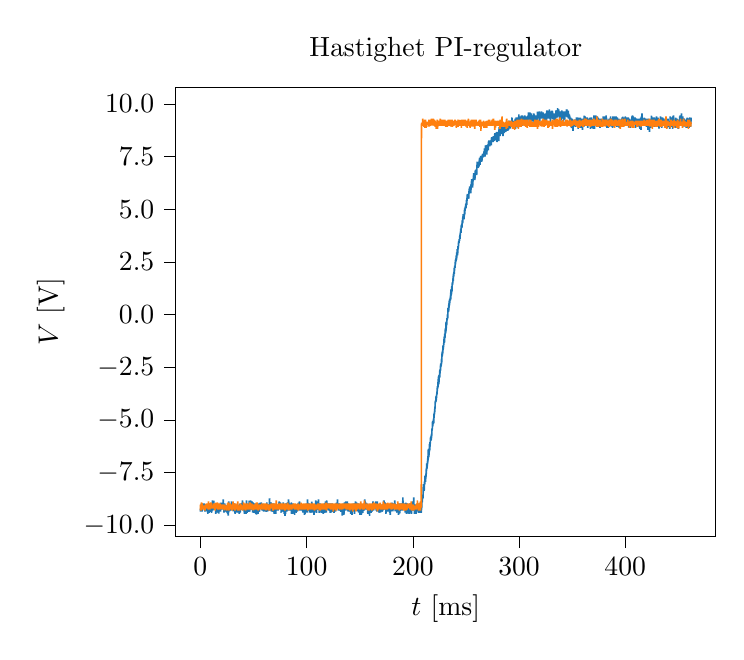
\begin{tikzpicture}

\definecolor{darkgray176}{RGB}{176,176,176}
\definecolor{darkorange25512714}{RGB}{255,127,14}
\definecolor{steelblue31119180}{RGB}{31,119,180}

\begin{axis}[
tick align=outside,
tick pos=left,
title={Hastighet PI-regulator},
x grid style={darkgray176},
xlabel={\(\displaystyle t\) [ms]},
xmin=-23.09538, xmax=485.00298,
xtick style={color=black},
xtick={-100,0,100,200,300,400,500},
xticklabels={
  \(\displaystyle {\ensuremath{-}100}\),
  \(\displaystyle {0}\),
  \(\displaystyle {100}\),
  \(\displaystyle {200}\),
  \(\displaystyle {300}\),
  \(\displaystyle {400}\),
  \(\displaystyle {500}\)
},
y grid style={darkgray176},
ylabel={\(\displaystyle V\) [V]},
ymin=-10.512697, ymax=10.756837,
ytick style={color=black},
ytick={-12.5,-10,-7.5,-5,-2.5,0,2.5,5,7.5,10,12.5},
yticklabels={
  \(\displaystyle {\ensuremath{-}12.5}\),
  \(\displaystyle {\ensuremath{-}10.0}\),
  \(\displaystyle {\ensuremath{-}7.5}\),
  \(\displaystyle {\ensuremath{-}5.0}\),
  \(\displaystyle {\ensuremath{-}2.5}\),
  \(\displaystyle {0.0}\),
  \(\displaystyle {2.5}\),
  \(\displaystyle {5.0}\),
  \(\displaystyle {7.5}\),
  \(\displaystyle {10.0}\),
  \(\displaystyle {12.5}\)
}
]
\addplot [semithick, steelblue31119180]
table {%
0 -9.2041
0.0923999999997704 -9.35059
0.184799999999985 -9.2041
0.277199999999755 -9.30176
0.36959999999997 -9.30176
0.46199999999974 -9.30176
0.554399999999955 -9.15527
0.646799999999725 -9.2041
0.73919999999994 -9.2041
0.83159999999971 -9.15527
0.923999999999925 -9.10645
1.0163999999997 -8.95996
1.10879999999991 -9.00879
1.20119999999968 -9.2041
1.29359999999989 -9.25293
1.38599999999967 -9.05762
1.47839999999988 -9.25293
1.57079999999965 -9.35059
1.66319999999986 -9.25293
1.75559999999964 -9.10645
1.84799999999985 -9.2041
1.94039999999962 -9.2041
2.03279999999983 -9.30176
2.12519999999961 -9.2041
2.21759999999982 -9.10645
2.30999999999959 -9.05762
2.4023999999998 -9.10645
2.49479999999958 -9.00879
2.58719999999979 -9.10645
2.6796 -9.10645
2.77199999999977 -8.95996
2.86439999999999 -9.15527
2.95679999999976 -9.05762
3.04919999999997 -9.10645
3.14159999999974 -9.10645
3.23399999999996 -9.15527
3.32639999999973 -9.15527
3.41879999999994 -9.10645
3.51119999999971 -9.00879
3.60359999999993 -9.00879
3.6959999999997 -8.95996
3.78839999999991 -9.15527
3.88079999999968 -9.05762
3.9731999999999 -9.10645
4.06559999999967 -9.15527
4.15799999999988 -9.10645
4.25039999999965 -9.35059
4.34279999999987 -9.2041
4.43519999999964 -9.25293
4.52759999999985 -9.2041
4.61999999999962 -9.05762
4.71239999999984 -9.10645
4.80479999999961 -9.10645
4.89719999999982 -9.00879
4.98959999999959 -9.05762
5.08199999999981 -9.2041
5.17439999999958 -9.15527
5.26679999999979 -9.10645
5.35920000000001 -9.25293
5.45159999999978 -9.30176
5.54399999999999 -9.30176
5.63639999999976 -9.10645
5.72879999999998 -9.25293
5.82119999999975 -9.30176
5.91359999999996 -9.10645
6.00599999999973 -9.05762
6.09839999999995 -9.15527
6.19079999999972 -9.05762
6.28319999999993 -9.10645
6.3755999999997 -9.2041
6.46799999999992 -9.05762
6.56039999999969 -9.2041
6.6527999999999 -9.25293
6.74519999999967 -9.30176
6.83759999999989 -9.39941
6.92999999999966 -9.30176
7.02239999999987 -9.44824
7.11479999999964 -9.30176
7.20719999999986 -9.15527
7.29959999999963 -9.10645
7.39199999999984 -9.25293
7.48439999999961 -9.05762
7.57679999999983 -9.15527
7.6691999999996 -9.25293
7.76159999999981 -9.30176
7.85399999999958 -9.39941
7.9463999999998 -9.15527
8.03880000000001 -9.30176
8.13119999999978 -9.39941
8.2236 -9.35059
8.31599999999977 -9.25293
8.40839999999998 -9.2041
8.50079999999975 -9.30176
8.59319999999997 -9.30176
8.68559999999974 -8.95996
8.77799999999995 -9.05762
8.87039999999972 -9.00879
8.96279999999994 -9.2041
9.05519999999971 -9.15527
9.14759999999992 -9.30176
9.23999999999969 -9.30176
9.33239999999991 -9.25293
9.42479999999968 -9.25293
9.51719999999989 -9.30176
9.60959999999966 -9.15527
9.70199999999988 -9.30176
9.79439999999965 -9.35059
9.88679999999986 -9.2041
9.97919999999963 -9.05762
10.0715999999998 -9.10645
10.1639999999996 -9.10645
10.2563999999998 -9.30176
10.3487999999996 -9.2041
10.4411999999998 -9.30176
10.5335999999996 -9.39941
10.6259999999998 -9.2041
10.7184 -9.35059
10.8107999999998 -9.15527
10.9032 -8.95996
10.9955999999998 -9.10645
11.088 -9.15527
11.1803999999998 -9.10645
11.2728 -8.81348
11.3651999999997 -8.95996
11.4576 -8.95996
11.5499999999997 -9.05762
11.6423999999999 -9.10645
11.7347999999997 -9.30176
11.8271999999999 -9.15527
11.9195999999997 -9.2041
12.0119999999999 -9.05762
12.1043999999997 -9.00879
12.1967999999999 -9.10645
12.2891999999997 -9.15527
12.3815999999999 -9.10645
12.4739999999997 -8.95996
12.5663999999999 -8.8623
12.6587999999996 -8.8623
12.7511999999999 -9.10645
12.8435999999996 -9.10645
12.9359999999998 -9.10645
13.0283999999996 -9.15527
13.1207999999998 -9.15527
13.2131999999996 -9.25293
13.3055999999998 -9.2041
13.3979999999996 -9.2041
13.4903999999998 -9.2041
13.5828 -9.05762
13.6751999999998 -9.25293
13.7676 -9.10645
13.8599999999998 -9.10645
13.9524 -9.10645
14.0447999999997 -9.10645
14.1372 -9.2041
14.2295999999997 -9.15527
14.3219999999999 -9.2041
14.4143999999997 -9.44824
14.5067999999999 -9.15527
14.5991999999997 -9.05762
14.6915999999999 -9.2041
14.7839999999997 -9.39941
14.8763999999999 -9.2041
14.9687999999997 -9.2041
15.0611999999999 -9.25293
15.1535999999997 -9.15527
15.2459999999999 -8.95996
15.3383999999996 -9.10645
15.4307999999999 -9.30176
15.5231999999996 -9.10645
15.6155999999998 -9.2041
15.7079999999996 -9.30176
15.8003999999998 -9.30176
15.8927999999996 -9.2041
15.9851999999998 -9.35059
16.0775999999996 -9.35059
16.1699999999998 -9.35059
16.2624 -9.25293
16.3547999999998 -9.15527
16.4472 -9.10645
16.5395999999998 -9.2041
16.632 -9.30176
16.7243999999998 -9.35059
16.8168 -9.10645
16.9091999999997 -9.30176
17.0016 -9.35059
17.0939999999997 -9.39941
17.1863999999999 -9.30176
17.2787999999997 -9.39941
17.3711999999999 -9.39941
17.4635999999997 -9.30176
17.5559999999999 -9.00879
17.6483999999997 -9.25293
17.7407999999999 -9.05762
17.8331999999997 -9.00879
17.9255999999999 -9.25293
18.0179999999996 -9.10645
18.1103999999999 -9.2041
18.2027999999996 -9.25293
18.2951999999998 -9.30176
18.3875999999996 -9.2041
18.4799999999998 -9.25293
18.5723999999996 -9.25293
18.6647999999998 -9.2041
18.7571999999996 -9.10645
18.8495999999998 -9.35059
18.942 -8.95996
19.0343999999998 -8.95996
19.1268 -9.25293
19.2191999999998 -9.2041
19.3116 -9.00879
19.4039999999998 -9.2041
19.4964 -9.25293
19.5887999999997 -9.10645
19.6812 -9.2041
19.7735999999997 -9.25293
19.8659999999999 -9.2041
19.9583999999997 -9.25293
20.0507999999999 -9.05762
20.1431999999997 -9.15527
20.2355999999999 -9.10645
20.3279999999997 -9.10645
20.4203999999999 -9.15527
20.5127999999997 -9.00879
20.6051999999999 -8.95996
20.6975999999996 -8.95996
20.7899999999999 -9.10645
20.8823999999996 -8.95996
20.9747999999998 -9.2041
21.0671999999996 -9.2041
21.1595999999998 -9.00879
21.2519999999996 -9.00879
21.3443999999998 -9.15527
21.4367999999996 -8.91113
21.5291999999998 -8.76465
21.6216 -8.91113
21.7139999999998 -9.10645
21.8064 -9.15527
21.8987999999998 -9.25293
21.9912 -9.15527
22.0835999999998 -9.25293
22.176 -9.2041
22.2683999999997 -9.39941
22.3608 -9.2041
22.4531999999997 -9.2041
22.5455999999999 -9.15527
22.6379999999997 -9.05762
22.7303999999999 -9.25293
22.8227999999997 -8.95996
22.9151999999999 -9.00879
23.0075999999997 -9.2041
23.0999999999999 -9.05762
23.1923999999997 -9.15527
23.2847999999999 -9.30176
23.3771999999997 -9.30176
23.4695999999999 -9.35059
23.5619999999996 -9.05762
23.6543999999999 -9.2041
23.7467999999996 -9.30176
23.8391999999998 -9.2041
23.9315999999996 -9.05762
24.0239999999998 -9.15527
24.1163999999996 -9.25293
24.2087999999998 -9.15527
24.3011999999996 -9.10645
24.3935999999998 -9.30176
24.486 -9.30176
24.5783999999998 -9.25293
24.6708 -9.2041
24.7631999999998 -9.35059
24.8556 -9.35059
24.9479999999997 -9.35059
25.0404 -9.30176
25.1327999999997 -9.2041
25.2251999999999 -9.2041
25.3175999999997 -9.25293
25.4099999999999 -9.2041
25.5023999999997 -9.05762
25.5947999999999 -9.2041
25.6871999999997 -9.44824
25.7795999999999 -9.2041
25.8719999999997 -9.39941
25.9643999999999 -9.30176
26.0567999999997 -9.25293
26.1491999999999 -9.49707
26.2415999999996 -9.49707
26.3339999999999 -9.35059
26.4263999999996 -9.39941
26.5187999999998 -9.05762
26.6111999999996 -8.8623
26.7035999999998 -8.95996
26.7959999999996 -9.05762
26.8883999999998 -9.2041
26.9807999999996 -9.25293
27.0731999999998 -9.10645
27.1656 -9.2041
27.2579999999998 -9.30176
27.3504 -9.25293
27.4427999999998 -9.30176
27.5352 -9.30176
27.6275999999998 -9.10645
27.72 -9.15527
27.8123999999997 -9.25293
27.9048 -9.15527
27.9971999999997 -9.10645
28.0895999999999 -9.10645
28.1819999999997 -9.00879
28.2743999999999 -9.10645
28.3667999999997 -9.30176
28.4591999999999 -9.2041
28.5515999999997 -9.2041
28.6439999999999 -9.30176
28.7363999999997 -9.10645
28.8287999999999 -9.15527
28.9211999999996 -9.2041
29.0135999999999 -9.2041
29.1059999999996 -9.05762
29.1983999999998 -9.00879
29.2907999999996 -8.8623
29.3831999999998 -9.05762
29.4755999999996 -9.00879
29.5679999999998 -9.00879
29.6603999999996 -8.95996
29.7527999999998 -9.2041
29.8452 -9.10645
29.9375999999998 -9.05762
30.03 -9.10645
30.1223999999998 -9.10645
30.2148 -9.05762
30.3071999999998 -8.95996
30.3996 -9.00879
30.4919999999997 -9.00879
30.5844 -8.91113
30.6767999999997 -9.10645
30.7691999999999 -9.10645
30.8615999999997 -9.00879
30.9539999999999 -9.30176
31.0463999999997 -9.30176
31.1387999999999 -9.30176
31.2311999999997 -9.25293
31.3235999999999 -9.25293
31.4159999999997 -9.15527
31.5083999999999 -9.15527
31.6007999999997 -9.25293
31.6931999999999 -9.10645
31.7855999999996 -9.10645
31.8779999999999 -8.95996
31.9703999999996 -9.2041
32.0627999999998 -9.10645
32.1551999999996 -9.25293
32.2475999999998 -9.25293
32.3399999999996 -9.2041
32.4323999999998 -9.39941
32.5247999999996 -9.30176
32.6171999999998 -9.39941
32.7096 -9.44824
32.8019999999998 -9.30176
32.8944 -9.25293
32.9867999999998 -9.05762
33.0792 -9.10645
33.1715999999997 -9.10645
33.264 -9.2041
33.3563999999997 -9.2041
33.4487999999999 -9.35059
33.5411999999997 -9.15527
33.6335999999999 -9.35059
33.7259999999997 -9.30176
33.8183999999999 -9.2041
33.9107999999997 -9.30176
34.0031999999999 -9.15527
34.0955999999997 -9.30176
34.1879999999999 -9.2041
34.2803999999997 -9.05762
34.3727999999999 -9.05762
34.4651999999996 -9.30176
34.5575999999999 -9.2041
34.6499999999996 -9.25293
34.7423999999998 -9.25293
34.8347999999996 -9.39941
34.9271999999998 -9.2041
35.0195999999996 -9.30176
35.1119999999998 -9.25293
35.2043999999996 -9.30176
35.2967999999998 -9.30176
35.3892 -9.2041
35.4815999999998 -9.2041
35.574 -9.25293
35.6663999999998 -9.10645
35.7588 -9.15527
35.8511999999997 -9.2041
35.9436 -9.05762
36.0359999999997 -9.10645
36.1283999999999 -9.30176
36.2207999999997 -9.2041
36.3131999999999 -9.10645
36.4055999999997 -9.2041
36.4979999999999 -9.44824
36.5903999999997 -9.05762
36.6827999999999 -9.15527
36.7751999999997 -9.15527
36.8675999999999 -9.00879
36.9599999999997 -9.00879
37.0523999999999 -9.10645
37.1447999999996 -9.15527
37.2371999999999 -9.10645
37.3295999999996 -9.25293
37.4219999999998 -9.39941
37.5143999999996 -9.2041
37.6067999999998 -9.35059
37.6991999999996 -9.2041
37.7915999999998 -9.30176
37.8839999999996 -9.10645
37.9763999999998 -9.10645
38.0688 -9.2041
38.1611999999998 -9.05762
38.2536 -9.00879
38.3459999999998 -9.00879
38.4384 -9.05762
38.5307999999998 -8.95996
38.6232 -9.05762
38.7155999999997 -9.10645
38.808 -9.25293
38.9003999999997 -9.10645
38.9927999999999 -9.10645
39.0851999999997 -9.00879
39.1775999999999 -9.10645
39.2699999999997 -8.95996
39.3623999999999 -8.95996
39.4547999999997 -8.95996
39.5471999999999 -8.81348
39.6395999999997 -9.10645
39.7319999999999 -9.10645
39.8243999999996 -9.10645
39.9167999999999 -9.2041
40.0091999999996 -9.25293
40.1015999999998 -9.25293
40.1939999999996 -9.25293
40.2863999999998 -9.25293
40.3787999999996 -9.25293
40.4711999999998 -9.2041
40.5635999999996 -9.00879
40.6559999999998 -9.10645
40.7484 -9.05762
40.8407999999998 -9.05762
40.9332 -9.10645
41.0255999999998 -9.10645
41.118 -9.10645
41.2103999999998 -9.35059
41.3028 -9.30176
41.3951999999997 -9.44824
41.4876 -9.2041
41.5799999999997 -9.39941
41.6723999999999 -9.15527
41.7647999999997 -9.05762
41.8571999999999 -9.10645
41.9495999999997 -9.25293
42.0419999999999 -9.10645
42.1343999999997 -9.15527
42.2267999999999 -9.2041
42.3191999999997 -9.30176
42.4115999999999 -9.35059
42.5039999999996 -9.15527
42.5963999999999 -9.25293
42.6887999999996 -9.25293
42.7811999999999 -9.30176
42.8735999999996 -9.30176
42.9659999999998 -9.44824
43.0583999999996 -9.25293
43.1507999999998 -9.2041
43.2431999999996 -9.00879
43.3355999999998 -8.81348
43.4279999999996 -8.95996
43.5203999999998 -9.10645
43.6128 -9.2041
43.7051999999998 -9.30176
43.7976 -9.39941
43.8899999999998 -9.30176
43.9824 -9.35059
44.0747999999997 -9.30176
44.1672 -9.25293
44.2595999999997 -9.2041
44.3519999999999 -9.35059
44.4443999999997 -9.10645
44.5367999999999 -9.00879
44.6291999999997 -9.00879
44.7215999999999 -9.05762
44.8139999999997 -9.05762
44.9063999999999 -9.15527
44.9987999999997 -9.25293
45.0911999999999 -9.25293
45.1835999999997 -9.30176
45.2759999999999 -9.35059
45.3683999999996 -9.30176
45.4607999999999 -9.05762
45.5531999999996 -9.2041
45.6455999999998 -9.25293
45.7379999999996 -9.10645
45.8303999999998 -9.00879
45.9227999999996 -8.8623
46.0151999999998 -8.8623
46.1075999999996 -9.10645
46.1999999999998 -9.2041
46.2924 -9.30176
46.3847999999998 -9.35059
46.4772 -9.15527
46.5695999999998 -9.10645
46.662 -9.15527
46.7543999999997 -9.15527
46.8468 -9.2041
46.9391999999997 -9.10645
47.0316 -9.15527
47.1239999999997 -9.05762
47.2163999999999 -8.95996
47.3087999999997 -8.81348
47.4011999999999 -9.00879
47.4935999999997 -9.10645
47.5859999999999 -9.10645
47.6783999999997 -9.25293
47.7707999999999 -9.00879
47.8631999999997 -9.10645
47.9555999999999 -9.10645
48.0479999999996 -9.05762
48.1403999999999 -9.2041
48.2327999999996 -9.15527
48.3251999999998 -9.05762
48.4175999999996 -8.91113
48.5099999999998 -8.8623
48.6023999999996 -9.10645
48.6947999999998 -9.10645
48.7871999999996 -9.15527
48.8795999999998 -9.10645
48.972 -9.2041
49.0643999999998 -9.15527
49.1568 -9.39941
49.2491999999998 -9.15527
49.3416 -9.30176
49.4339999999998 -9.30176
49.5264 -9.30176
49.6187999999997 -8.91113
49.7112 -8.95996
49.8035999999997 -9.10645
49.8959999999999 -9.15527
49.9883999999997 -9.10645
50.0807999999999 -9.15527
50.1731999999997 -9.05762
50.2655999999999 -9.30176
50.3579999999997 -9.39941
50.4503999999999 -9.15527
50.5427999999997 -9.30176
50.6351999999999 -9.35059
50.7275999999997 -9.30176
50.8199999999999 -9.25293
50.9123999999996 -9.30176
51.0047999999998 -9.15527
51.0971999999996 -9.30176
51.1895999999998 -8.95996
51.2819999999996 -9.10645
51.3743999999998 -9.25293
51.4667999999996 -9.35059
51.5591999999998 -9.39941
51.6515999999996 -9.15527
51.7439999999998 -9.2041
51.8364 -9.35059
51.9287999999998 -9.25293
52.0212 -9.44824
52.1135999999998 -9.2041
52.206 -9.05762
52.2983999999997 -9.15527
52.3908 -9.30176
52.4831999999997 -9.15527
52.5755999999999 -9.25293
52.6679999999997 -9.25293
52.7603999999999 -9.30176
52.8527999999997 -9.44824
52.9451999999999 -9.44824
53.0375999999997 -9.30176
53.1299999999999 -9.35059
53.2223999999997 -9.30176
53.3147999999999 -9.30176
53.4071999999997 -9.39941
53.4995999999999 -9.00879
53.5919999999996 -9.2041
53.6843999999999 -9.05762
53.7767999999996 -9.25293
53.8691999999998 -9.2041
53.9615999999996 -9.30176
54.0539999999998 -9.15527
54.1463999999996 -9.15527
54.2387999999998 -9.44824
54.3311999999996 -9.05762
54.4235999999998 -9.30176
54.516 -9.10645
54.6083999999998 -9.25293
54.7008 -9.00879
54.7931999999998 -8.95996
54.8856 -9.10645
54.9779999999998 -9.15527
55.0704 -9.05762
55.1627999999997 -9.30176
55.2551999999999 -9.30176
55.3475999999997 -9.35059
55.4399999999999 -9.00879
55.5323999999997 -9.30176
55.6247999999999 -9.35059
55.7171999999997 -9.25293
55.8095999999999 -9.10645
55.9019999999997 -9.10645
55.9943999999999 -9.05762
56.0867999999997 -9.00879
56.1791999999999 -8.95996
56.2715999999996 -8.95996
56.3639999999999 -8.95996
56.4563999999996 -9.10645
56.5487999999998 -9.10645
56.6411999999996 -9.10645
56.7335999999998 -9.10645
56.8259999999996 -9.10645
56.9183999999998 -9.00879
57.0107999999996 -9.00879
57.1031999999998 -9.10645
57.1956 -9.10645
57.2879999999998 -9.00879
57.3804 -8.91113
57.4727999999998 -9.10645
57.5652 -9.00879
57.6575999999998 -9.10645
57.75 -9.10645
57.8423999999997 -9.15527
57.9348 -9.25293
58.0271999999997 -9.2041
58.1195999999999 -9.30176
58.2119999999997 -9.10645
58.3043999999999 -9.2041
58.3967999999997 -9.25293
58.4891999999999 -9.10645
58.5815999999997 -9.10645
58.6739999999999 -9.15527
58.7663999999997 -9.00879
58.8587999999999 -9.00879
58.9511999999996 -9.15527
59.0435999999999 -9.15527
59.1359999999996 -9.10645
59.2283999999999 -9.25293
59.3207999999996 -9.30176
59.4131999999998 -9.30176
59.5055999999996 -9.2041
59.5979999999998 -9.30176
59.6903999999996 -9.2041
59.7827999999998 -9.35059
59.8752 -9.15527
59.9675999999998 -9.00879
60.06 -9.05762
60.1523999999998 -9.05762
60.2448 -9.15527
60.3371999999998 -9.30176
60.4296 -9.30176
60.5219999999997 -9.30176
60.6144 -9.25293
60.7067999999997 -9.30176
60.7991999999999 -9.30176
60.8915999999997 -9.25293
60.9839999999999 -9.15527
61.0763999999997 -9.30176
61.1687999999999 -9.25293
61.2611999999997 -9.15527
61.3535999999999 -9.10645
61.4459999999997 -9.2041
61.5383999999999 -9.15527
61.6307999999997 -9.30176
61.7231999999999 -9.25293
61.8155999999996 -9.35059
61.9079999999999 -9.30176
62.0003999999996 -9.30176
62.0927999999998 -9.25293
62.1851999999996 -9.30176
62.2775999999998 -9.35059
62.3699999999996 -9.30176
62.4623999999998 -9.10645
62.5547999999996 -8.91113
62.6471999999998 -9.10645
62.7396 -9.10645
62.8319999999998 -9.25293
62.9244 -9.05762
63.0167999999998 -9.15527
63.1092 -9.30176
63.2015999999997 -9.25293
63.294 -9.30176
63.3863999999997 -9.30176
63.4787999999999 -9.25293
63.5711999999997 -9.2041
63.6635999999999 -9.10645
63.7559999999997 -9.15527
63.8483999999999 -9.00879
63.9407999999997 -9.10645
64.0331999999999 -9.30176
64.1255999999997 -9.15527
64.2179999999999 -9.30176
64.3103999999997 -9.2041
64.4027999999999 -9.30176
64.4951999999996 -9.15527
64.5875999999999 -9.30176
64.6799999999996 -9.2041
64.7723999999998 -9.30176
64.8647999999996 -9.15527
64.9571999999998 -8.95996
65.0495999999996 -8.71582
65.1419999999998 -8.76465
65.2343999999996 -8.95996
65.3267999999998 -8.95996
65.4192 -9.10645
65.5115999999998 -9.00879
65.604 -9.15527
65.6963999999998 -9.30176
65.7888 -9.2041
65.8811999999998 -9.15527
65.9736 -9.15527
66.0659999999997 -9.00879
66.1583999999999 -9.10645
66.2507999999997 -8.95996
66.3431999999999 -9.15527
66.4355999999997 -9.05762
66.5279999999999 -8.91113
66.6203999999997 -9.15527
66.7127999999999 -9.25293
66.8051999999997 -9.2041
66.8975999999999 -9.25293
66.9899999999997 -9.35059
67.0823999999999 -9.2041
67.1747999999996 -9.25293
67.2671999999999 -9.2041
67.3595999999996 -9.30176
67.4519999999998 -9.25293
67.5443999999996 -9.10645
67.6367999999998 -9.05762
67.7291999999996 -8.95996
67.8215999999998 -9.25293
67.9139999999996 -9.00879
68.0063999999998 -9.15527
68.0988 -9.30176
68.1911999999998 -9.30176
68.2836 -9.30176
68.3759999999998 -9.2041
68.4684 -9.30176
68.5607999999998 -9.35059
68.6532 -9.25293
68.7455999999997 -9.2041
68.838 -9.15527
68.9303999999997 -9.2041
69.0227999999999 -9.05762
69.1151999999997 -8.95996
69.2075999999999 -9.10645
69.2999999999997 -9.35059
69.3923999999999 -9.39941
69.4847999999997 -9.44824
69.5771999999999 -9.39941
69.6695999999997 -9.25293
69.7619999999999 -9.30176
69.8543999999997 -9.30176
69.9467999999999 -9.00879
70.0391999999996 -9.2041
70.1315999999998 -9.10645
70.2239999999996 -9.00879
70.3163999999998 -9.10645
70.4087999999996 -9.2041
70.5011999999998 -9.10645
70.5935999999996 -9.2041
70.6859999999998 -9.35059
70.7783999999996 -9.39941
70.8707999999998 -9.30176
70.9632 -9.44824
71.0555999999998 -9.30176
71.148 -9.25293
71.2403999999998 -9.05762
71.3328 -9.25293
71.4251999999997 -9.00879
71.5176 -9.05762
71.6099999999997 -9.00879
71.7023999999999 -9.25293
71.7947999999997 -9.25293
71.8871999999999 -9.2041
71.9795999999997 -9.15527
72.0719999999999 -9.2041
72.1643999999997 -9.15527
72.2567999999999 -9.15527
72.3491999999997 -9.30176
72.4415999999999 -9.10645
72.5339999999997 -9.30176
72.6263999999999 -9.15527
72.7187999999996 -9.00879
72.8111999999999 -9.10645
72.9035999999996 -9.00879
72.9959999999998 -9.25293
73.0883999999996 -9.30176
73.1807999999998 -9.2041
73.2731999999996 -9.05762
73.3655999999998 -9.2041
73.4579999999996 -9.2041
73.5503999999998 -9.15527
73.6428 -9.10645
73.7351999999998 -9.15527
73.8276 -9.15527
73.9199999999998 -8.95996
74.0124 -8.95996
74.1047999999998 -8.95996
74.1972 -8.8623
74.2895999999997 -9.00879
74.3819999999999 -9.00879
74.4743999999997 -8.95996
74.5667999999999 -9.10645
74.6591999999997 -9.00879
74.7515999999999 -9.10645
74.8439999999997 -8.95996
74.9363999999999 -9.10645
75.0287999999997 -9.05762
75.1211999999999 -8.95996
75.2135999999997 -9.05762
75.3059999999999 -8.91113
75.3983999999996 -9.00879
75.4907999999999 -9.00879
75.5831999999996 -9.10645
75.6755999999998 -9.10645
75.7679999999996 -9.10645
75.8603999999998 -9.25293
75.9527999999996 -9.15527
76.0451999999998 -9.25293
76.1375999999996 -9.39941
76.2299999999998 -9.2041
76.3224 -9.10645
76.4147999999998 -9.10645
76.5072 -9.10645
76.5995999999998 -9.05762
76.692 -9.10645
76.7843999999997 -9.15527
76.8768 -9.15527
76.9691999999997 -9.15527
77.0616 -9.25293
77.1539999999997 -9.30176
77.2463999999999 -9.35059
77.3387999999997 -9.10645
77.4311999999999 -9.30176
77.5235999999997 -9.25293
77.6159999999999 -9.35059
77.7083999999997 -9.15527
77.8007999999999 -9.15527
77.8931999999997 -9.2041
77.9855999999999 -8.91113
78.0779999999996 -9.25293
78.1703999999999 -9.2041
78.2627999999996 -9.25293
78.3551999999999 -9.15527
78.4475999999996 -9.30176
78.5399999999998 -9.30176
78.6323999999996 -9.35059
78.7247999999998 -9.2041
78.8171999999996 -9.44824
78.9095999999998 -9.25293
79.002 -9.15527
79.0943999999998 -9.10645
79.1868 -9.2041
79.2791999999998 -9.00879
79.3716 -9.30176
79.4639999999998 -9.25293
79.5564 -9.30176
79.6487999999997 -9.5459
79.7412 -9.30176
79.8335999999997 -9.39941
79.9259999999999 -9.25293
80.0183999999997 -9.35059
80.1107999999999 -9.44824
80.2031999999997 -9.25293
80.2955999999999 -9.30176
80.3879999999997 -8.95996
80.4803999999999 -9.10645
80.5727999999997 -9.05762
80.6651999999999 -9.25293
80.7575999999997 -9.25293
80.8499999999999 -9.25293
80.9423999999996 -9.2041
81.0347999999998 -9.30176
81.1271999999996 -9.25293
81.2195999999998 -9.2041
81.3119999999996 -9.35059
81.4043999999998 -9.2041
81.4967999999996 -9.15527
81.5891999999998 -9.2041
81.6815999999996 -9.25293
81.7739999999998 -9.00879
81.8664 -8.91113
81.9587999999998 -9.15527
82.0512 -9.10645
82.1435999999998 -9.30176
82.236 -9.2041
82.3283999999997 -9.25293
82.4208 -9.10645
82.5131999999997 -9.2041
82.6056 -9.15527
82.6979999999997 -9.30176
82.7903999999999 -9.05762
82.8827999999997 -9.10645
82.9751999999999 -8.76465
83.0675999999997 -8.95996
83.1599999999999 -8.91113
83.2523999999997 -8.91113
83.3447999999999 -8.95996
83.4371999999996 -9.15527
83.5295999999999 -9.15527
83.6219999999996 -9.00879
83.7143999999999 -9.00879
83.8067999999996 -9.30176
83.8991999999998 -9.2041
83.9915999999996 -9.10645
84.0839999999998 -8.95996
84.1763999999996 -9.10645
84.2687999999998 -9.10645
84.3611999999996 -9.00879
84.4535999999998 -8.95996
84.546 -9.15527
84.6383999999998 -9.2041
84.7308 -9.15527
84.8231999999998 -9.2041
84.9156 -9.00879
85.0079999999998 -9.25293
85.1004 -9.25293
85.1927999999997 -9.15527
85.2851999999999 -9.15527
85.3775999999997 -9.15527
85.4699999999999 -9.05762
85.5623999999997 -9.05762
85.6547999999999 -8.91113
85.7471999999997 -9.15527
85.8395999999999 -9.44824
85.9319999999997 -9.35059
86.0243999999999 -9.15527
86.1167999999997 -9.25293
86.2091999999999 -9.25293
86.3015999999996 -9.15527
86.3939999999999 -9.44824
86.4863999999996 -9.35059
86.5787999999998 -9.30176
86.6711999999996 -9.30176
86.7635999999998 -9.30176
86.8559999999996 -9.15527
86.9483999999998 -8.95996
87.0407999999996 -9.00879
87.1331999999998 -9.10645
87.2256 -9.25293
87.3179999999998 -9.30176
87.4104 -9.25293
87.5027999999998 -9.35059
87.5952 -9.30176
87.6875999999997 -9.05762
87.78 -9.15527
87.8723999999997 -9.15527
87.9648 -9.25293
88.0571999999997 -9.15527
88.1495999999999 -9.00879
88.2419999999997 -9.15527
88.3343999999999 -9.25293
88.4267999999997 -9.44824
88.5191999999999 -9.15527
88.6115999999997 -9.30176
88.7039999999999 -9.49707
88.7963999999997 -9.15527
88.8887999999999 -9.2041
88.9811999999996 -9.30176
89.0735999999999 -9.30176
89.1659999999996 -9.30176
89.2583999999999 -9.25293
89.3507999999996 -9.2041
89.4431999999998 -9.15527
89.5355999999996 -9.00879
89.6279999999998 -9.10645
89.7203999999996 -9.15527
89.8127999999998 -9.10645
89.9052 -9.30176
89.9975999999998 -9.15527
90.09 -9.39941
90.1823999999998 -9.30176
90.2748 -9.30176
90.3671999999998 -9.15527
90.4596 -9.15527
90.5519999999997 -9.10645
90.6444 -9.10645
90.7367999999997 -9.00879
90.8291999999999 -9.05762
90.9215999999997 -9.05762
91.0139999999999 -9.30176
91.1063999999997 -9.25293
91.1987999999999 -9.2041
91.2911999999997 -9.35059
91.3835999999999 -9.25293
91.4759999999997 -9.25293
91.5683999999999 -9.2041
91.6607999999997 -9.25293
91.7531999999999 -9.10645
91.8455999999996 -9.15527
91.9379999999998 -9.05762
92.0303999999996 -8.95996
92.1227999999998 -9.05762
92.2151999999996 -9.05762
92.3075999999998 -8.95996
92.3999999999996 -8.95996
92.4923999999998 -9.10645
92.5847999999996 -9.10645
92.6771999999998 -9.00879
92.7696 -9.00879
92.8619999999998 -9.00879
92.9544 -9.05762
93.0467999999998 -9.00879
93.1392 -9.00879
93.2315999999997 -8.8623
93.324 -8.95996
93.4163999999997 -8.95996
93.5088 -8.95996
93.6011999999997 -9.10645
93.6935999999999 -9.10645
93.7859999999997 -9.30176
93.8783999999999 -9.2041
93.9707999999997 -9.10645
94.0631999999999 -9.25293
94.1555999999997 -9.2041
94.2479999999999 -9.25293
94.3403999999997 -9.25293
94.4327999999999 -9.2041
94.5251999999996 -9.15527
94.6175999999999 -9.00879
94.7099999999996 -9.05762
94.8023999999998 -9.2041
94.8947999999996 -9.2041
94.9871999999998 -9.2041
95.0795999999996 -9.05762
95.1719999999998 -9.25293
95.2643999999996 -9.30176
95.3567999999998 -9.2041
95.4492 -9.30176
95.5415999999998 -9.25293
95.634 -9.30176
95.7263999999998 -9.05762
95.8188 -9.05762
95.9111999999998 -9.00879
96.0036 -9.2041
96.0959999999997 -9.25293
96.1883999999999 -9.10645
96.2807999999997 -9.35059
96.3731999999999 -9.30176
96.4655999999997 -9.2041
96.5579999999999 -9.35059
96.6503999999997 -9.35059
96.7427999999999 -9.25293
96.8351999999997 -9.35059
96.9275999999999 -9.25293
97.0199999999997 -9.25293
97.1123999999999 -9.2041
97.2047999999997 -9.10645
97.2971999999999 -9.10645
97.3895999999996 -9.25293
97.4819999999998 -9.30176
97.5743999999996 -9.35059
97.6667999999998 -9.30176
97.7591999999996 -9.35059
97.8515999999998 -9.30176
97.9439999999996 -9.49707
98.0363999999998 -9.30176
98.1288 -9.2041
98.2211999999998 -9.25293
98.3136 -9.05762
98.4059999999998 -9.10645
98.4984 -9.30176
98.5907999999998 -9.44824
98.6832 -9.15527
98.7755999999997 -9.30176
98.868 -9.25293
98.9603999999997 -9.30176
99.0527999999999 -9.2041
99.1451999999997 -9.25293
99.2375999999999 -9.15527
99.3299999999997 -9.30176
99.4223999999999 -9.25293
99.5147999999997 -9.15527
99.6071999999999 -9.15527
99.6995999999997 -9.00879
99.7919999999999 -9.00879
99.8843999999997 -9.15527
99.9767999999999 -9.25293
100.0692 -9.10645
100.1616 -9.30176
100.254 -9.2041
100.3464 -9.35059
100.4388 -9.35059
100.5312 -9.10645
100.6236 -9.00879
100.716 -9.15527
100.8084 -9.10645
100.9008 -8.76465
100.9932 -8.95996
101.0856 -8.95996
101.178 -8.95996
101.2704 -9.00879
101.3628 -8.95996
101.4552 -9.15527
101.5476 -9.15527
101.64 -9.10645
101.7324 -9.10645
101.8248 -9.00879
101.9172 -9.30176
102.0096 -8.95996
102.102 -9.10645
102.1944 -8.95996
102.2868 -9.05762
102.3792 -8.95996
102.4716 -9.10645
102.564 -9.10645
102.6564 -9.39941
102.7488 -9.05762
102.8412 -9.2041
102.9336 -9.2041
103.026 -9.15527
103.1184 -9.10645
103.2108 -9.2041
103.3032 -9.10645
103.3956 -9.25293
103.488 -9.10645
103.5804 -9.10645
103.6728 -9.2041
103.7652 -9.2041
103.8576 -9.25293
103.95 -9.15527
104.0424 -9.30176
104.1348 -9.30176
104.2272 -9.39941
104.3196 -9.15527
104.412 -9.2041
104.5044 -9.25293
104.5968 -9.2041
104.6892 -9.05762
104.7816 -9.25293
104.874 -8.91113
104.9664 -8.91113
105.0588 -9.10645
105.1512 -9.2041
105.2436 -9.30176
105.336 -9.2041
105.4284 -9.2041
105.5208 -9.35059
105.6132 -9.35059
105.7056 -9.10645
105.798 -9.30176
105.8904 -9.25293
105.9828 -9.00879
106.0752 -9.10645
106.1676 -9.30176
106.26 -9.10645
106.3524 -9.30176
106.4448 -9.30176
106.5372 -9.15527
106.6296 -9.39941
106.722 -9.35059
106.8144 -9.35059
106.9068 -9.49707
106.9992 -9.15527
107.0916 -9.44824
107.184 -9.15527
107.2764 -9.15527
107.3688 -9.10645
107.4612 -9.00879
107.5536 -9.25293
107.646 -9.15527
107.7384 -9.00879
107.8308 -9.30176
107.9232 -9.10645
108.0156 -9.10645
108.108 -9.2041
108.2004 -9.25293
108.2928 -9.25293
108.3852 -9.00879
108.4776 -9.05762
108.57 -9.10645
108.6624 -8.81348
108.7548 -9.05762
108.8472 -9.05762
108.9396 -9.15527
109.032 -9.35059
109.1244 -9.30176
109.2168 -9.2041
109.3092 -9.39941
109.4016 -9.35059
109.494 -9.2041
109.5864 -9.10645
109.6788 -9.10645
109.7712 -9.10645
109.8636 -9.15527
109.956 -9.10645
110.0484 -9.05762
110.1408 -8.95996
110.2332 -8.8623
110.3256 -9.10645
110.418 -9.10645
110.5104 -9.25293
110.6028 -9.00879
110.6952 -9.15527
110.7876 -9.05762
110.88 -9.00879
110.9724 -9.00879
111.0648 -9.10645
111.1572 -8.76465
111.2496 -8.95996
111.342 -9.00879
111.4344 -9.05762
111.5268 -9.15527
111.6192 -9.05762
111.7116 -9.05762
111.804 -9.30176
111.8964 -9.39941
111.9888 -9.30176
112.0812 -9.15527
112.1736 -9.39941
112.266 -9.30176
112.3584 -9.10645
112.4508 -9.00879
112.5432 -9.15527
112.6356 -8.95996
112.728 -9.10645
112.8204 -9.15527
112.9128 -9.15527
113.0052 -9.30176
113.0976 -9.35059
113.19 -9.15527
113.2824 -9.2041
113.3748 -9.25293
113.4672 -9.2041
113.5596 -9.30176
113.652 -9.25293
113.7444 -9.00879
113.8368 -9.10645
113.9292 -9.10645
114.0216 -9.10645
114.114 -9.30176
114.2064 -9.30176
114.2988 -9.39941
114.3912 -9.25293
114.4836 -9.30176
114.576 -9.30176
114.6684 -9.39941
114.7608 -9.25293
114.8532 -9.2041
114.9456 -9.15527
115.038 -9.00879
115.1304 -9.10645
115.2228 -9.15527
115.3152 -9.30176
115.4076 -9.35059
115.5 -9.10645
115.5924 -9.44824
115.6848 -9.2041
115.7772 -9.35059
115.8696 -9.30176
115.962 -9.30176
116.0544 -9.2041
116.1468 -9.30176
116.2392 -9.05762
116.3316 -9.10645
116.424 -9.00879
116.5164 -9.00879
116.6088 -9.25293
116.7012 -9.2041
116.7936 -9.39941
116.886 -9.30176
116.9784 -9.30176
117.0708 -9.30176
117.1632 -9.2041
117.2556 -9.05762
117.348 -9.2041
117.4404 -9.10645
117.5328 -9.10645
117.6252 -8.91113
117.7176 -8.8623
117.81 -9.05762
117.9024 -9.15527
117.9948 -9.10645
118.0872 -9.30176
118.1796 -9.30176
118.272 -9.35059
118.3644 -9.30176
118.4568 -9.35059
118.5492 -9.35059
118.6416 -9.2041
118.734 -9.25293
118.8264 -8.81348
118.9188 -8.8623
119.0112 -8.91113
119.1036 -9.00879
119.196 -8.95996
119.2884 -9.05762
119.3808 -8.95996
119.4732 -9.25293
119.5656 -9.10645
119.658 -9.15527
119.7504 -9.15527
119.8428 -9.10645
119.9352 -9.00879
120.0276 -8.95996
120.12 -9.05762
120.2124 -9.00879
120.3048 -8.95996
120.3972 -9.10645
120.4896 -8.95996
120.582 -9.00879
120.6744 -9.25293
120.7668 -9.30176
120.8592 -9.25293
120.9516 -9.30176
121.044 -9.10645
121.1364 -9.05762
121.2288 -9.2041
121.3212 -9.15527
121.4136 -9.00879
121.506 -8.95996
121.5984 -9.10645
121.6908 -9.15527
121.7832 -9.25293
121.8756 -9.2041
121.968 -9.2041
122.0604 -9.30176
122.1528 -9.39941
122.2452 -9.30176
122.3376 -9.2041
122.43 -9.15527
122.5224 -9.15527
122.6148 -9.15527
122.7072 -8.95996
122.7996 -9.25293
122.892 -9.2041
122.9844 -9.05762
123.0768 -9.15527
123.1692 -9.35059
123.2616 -9.35059
123.354 -9.25293
123.4464 -9.30176
123.5388 -9.25293
123.6312 -9.2041
123.7236 -9.30176
123.816 -9.15527
123.9084 -9.30176
124.0008 -8.95996
124.0932 -9.2041
124.1856 -9.15527
124.278 -9.2041
124.3704 -9.35059
124.4628 -9.30176
124.5552 -9.2041
124.6476 -9.25293
124.74 -9.30176
124.8324 -9.30176
124.9248 -9.15527
125.0172 -9.10645
125.1096 -9.15527
125.202 -9.00879
125.2944 -9.05762
125.3868 -9.10645
125.4792 -9.2041
125.5716 -9.10645
125.664 -9.10645
125.7564 -9.30176
125.8488 -9.39941
125.9412 -9.30176
126.0336 -9.00879
126.126 -9.30176
126.2184 -9.2041
126.3108 -9.05762
126.4032 -9.00879
126.4956 -9.05762
126.588 -9.10645
126.6804 -9.10645
126.7728 -9.00879
126.8652 -9.10645
126.9576 -9.15527
127.05 -9.10645
127.1424 -9.35059
127.2348 -9.15527
127.3272 -9.10645
127.4196 -9.10645
127.512 -9.15527
127.6044 -9.2041
127.6968 -9.10645
127.7892 -9.10645
127.8816 -9.00879
127.974 -8.95996
128.0664 -8.95996
128.1588 -9.00879
128.2512 -8.95996
128.3436 -9.15527
128.436 -9.00879
128.5284 -9.00879
128.6208 -9.00879
128.7132 -9.05762
128.8056 -9.10645
128.898 -9.10645
128.9904 -9.10645
129.0828 -8.76465
129.1752 -9.00879
129.2676 -9.00879
129.36 -8.95996
129.4524 -9.05762
129.5448 -9.15527
129.6372 -9.10645
129.7296 -9.2041
129.822 -9.10645
129.9144 -9.30176
130.0068 -9.10645
130.0992 -9.25293
130.1916 -9.10645
130.284 -9.2041
130.3764 -9.2041
130.4688 -9.15527
130.5612 -8.95996
130.6536 -9.10645
130.746 -9.15527
130.8384 -9.25293
130.9308 -9.10645
131.0232 -9.25293
131.1156 -9.30176
131.208 -9.05762
131.3004 -9.25293
131.3928 -9.25293
131.4852 -9.2041
131.5776 -9.25293
131.67 -9.10645
131.7624 -9.15527
131.8548 -9.25293
131.9472 -9.30176
132.0396 -9.30176
132.132 -9.10645
132.2244 -9.2041
132.3168 -9.30176
132.4092 -9.35059
132.5016 -9.30176
132.594 -9.30176
132.6864 -9.30176
132.7788 -9.30176
132.8712 -9.15527
132.9636 -9.10645
133.056 -9.15527
133.1484 -9.00879
133.2408 -9.15527
133.3332 -9.2041
133.4256 -9.30176
133.518 -9.49707
133.6104 -9.49707
133.7028 -9.49707
133.7952 -9.39941
133.8876 -9.30176
133.98 -9.35059
134.0724 -9.30176
134.1648 -9.00879
134.2572 -9.00879
134.3496 -9.00879
134.442 -9.00879
134.5344 -9.15527
134.6268 -9.30176
134.7192 -9.15527
134.8116 -9.30176
134.904 -9.30176
134.9964 -9.30176
135.0888 -9.49707
135.1812 -9.30176
135.2736 -9.10645
135.366 -9.10645
135.4584 -9.10645
135.5508 -9.05762
135.6432 -8.91113
135.7356 -9.15527
135.828 -9.15527
135.9204 -9.05762
136.0128 -9.25293
136.1052 -9.30176
136.1976 -9.25293
136.29 -9.30176
136.3824 -9.15527
136.4748 -9.05762
136.5672 -9.30176
136.6596 -9.2041
136.752 -9.05762
136.8444 -8.91113
136.9368 -8.8623
137.0292 -9.05762
137.1216 -8.8623
137.214 -9.05762
137.3064 -9.05762
137.3988 -8.95996
137.4912 -9.15527
137.5836 -9.2041
137.676 -9.2041
137.7684 -9.05762
137.8608 -9.15527
137.9532 -9.10645
138.0456 -9.10645
138.138 -8.91113
138.2304 -8.8623
138.3228 -9.00879
138.4152 -9.05762
138.5076 -9.25293
138.6 -9.2041
138.6924 -9.30176
138.7848 -9.25293
138.8772 -9.15527
138.9696 -9.30176
139.062 -9.15527
139.1544 -9.35059
139.2468 -9.15527
139.3392 -8.95996
139.4316 -9.00879
139.524 -9.2041
139.6164 -9.2041
139.7088 -9.25293
139.8012 -9.30176
139.8936 -9.25293
139.986 -9.30176
140.0784 -9.30176
140.1708 -9.30176
140.2632 -9.25293
140.3556 -9.30176
140.448 -9.30176
140.5404 -9.10645
140.6328 -9.10645
140.7252 -9.15527
140.8176 -9.10645
140.91 -9.10645
141.0024 -9.35059
141.0948 -9.30176
141.1872 -9.30176
141.2796 -9.35059
141.372 -9.25293
141.4644 -9.30176
141.5568 -9.44824
141.6492 -9.30176
141.7416 -9.25293
141.834 -9.10645
141.9264 -9.15527
142.0188 -9.10645
142.1112 -9.25293
142.2036 -9.30176
142.296 -9.30176
142.3884 -9.35059
142.4808 -9.30176
142.5732 -9.44824
142.6656 -9.49707
142.758 -9.39941
142.8504 -9.2041
142.9428 -9.2041
143.0352 -9.10645
143.1276 -9.30176
143.22 -9.00879
143.3124 -9.00879
143.4048 -9.10645
143.4972 -9.2041
143.5896 -9.15527
143.682 -9.15527
143.7744 -9.15527
143.8668 -9.30176
143.9592 -9.2041
144.0516 -9.30176
144.144 -9.30176
144.2364 -9.15527
144.3288 -9.10645
144.4212 -9.10645
144.5136 -9.00879
144.606 -9.10645
144.6984 -8.95996
144.7908 -9.2041
144.8832 -9.2041
144.9756 -9.05762
145.068 -9.44824
145.1604 -9.30176
145.2528 -9.05762
145.3452 -9.30176
145.4376 -9.30176
145.53 -9.25293
145.6224 -9.10645
145.7148 -9.00879
145.8072 -9.05762
145.8996 -8.95996
145.992 -8.8623
146.0844 -9.05762
146.1768 -9.00879
146.2692 -9.05762
146.3616 -9.15527
146.454 -9.05762
146.5464 -9.15527
146.6388 -9.15527
146.7312 -9.00879
146.8236 -8.91113
146.916 -9.10645
147.0084 -8.91113
147.1008 -9.05762
147.1932 -8.95996
147.2856 -9.10645
147.378 -9.25293
147.4704 -9.30176
147.5628 -9.00879
147.6552 -9.25293
147.7476 -9.30176
147.84 -9.30176
147.9324 -9.25293
148.0248 -9.15527
148.1172 -9.25293
148.2096 -9.00879
148.302 -9.00879
148.3944 -9.10645
148.4868 -9.00879
148.5792 -9.15527
148.6716 -8.95996
148.764 -9.05762
148.8564 -9.30176
148.9488 -9.2041
149.0412 -9.39941
149.1336 -9.15527
149.226 -9.05762
149.3184 -9.15527
149.4108 -9.39941
149.5032 -9.15527
149.5956 -9.2041
149.688 -9.10645
149.7804 -9.00879
149.8728 -9.05762
149.9652 -9.10645
150.0576 -9.30176
150.15 -9.2041
150.2424 -9.49707
150.3348 -9.30176
150.4272 -9.25293
150.5196 -9.25293
150.612 -9.39941
150.7044 -9.15527
150.7968 -9.30176
150.8892 -9.05762
150.9816 -9.10645
151.074 -9.05762
151.1664 -9.25293
151.2588 -9.30176
151.3512 -9.05762
151.4436 -9.49707
151.536 -9.30176
151.6284 -9.30176
151.7208 -9.44824
151.8132 -9.30176
151.9056 -9.30176
151.998 -9.05762
152.0904 -9.15527
152.1828 -9.05762
152.2752 -9.10645
152.3676 -9.2041
152.46 -9.15527
152.5524 -9.30176
152.6448 -9.25293
152.7372 -9.35059
152.8296 -9.39941
152.922 -9.30176
153.0144 -9.30176
153.1068 -9.2041
153.1992 -9.15527
153.2916 -9.05762
153.384 -9.05762
153.4764 -9.05762
153.5688 -9.10645
153.6612 -9.00879
153.7536 -9.25293
153.846 -9.15527
153.9384 -9.2041
154.0308 -9.2041
154.1232 -9.15527
154.2156 -9.10645
154.308 -9.30176
154.4004 -9.05762
154.4928 -9.25293
154.5852 -9.2041
154.6776 -8.95996
154.77 -8.76465
154.8624 -8.8623
154.9548 -8.91113
155.0472 -8.8623
155.1396 -9.10645
155.232 -9.00879
155.3244 -9.15527
155.4168 -9.00879
155.5092 -9.2041
155.6016 -8.95996
155.694 -9.15527
155.7864 -9.10645
155.8788 -9.10645
155.9712 -9.00879
156.0636 -8.95996
156.156 -8.95996
156.2484 -9.05762
156.3408 -9.2041
156.4332 -9.25293
156.5256 -9.10645
156.618 -9.15527
156.7104 -9.25293
156.8028 -9.10645
156.8952 -9.10645
156.9876 -9.25293
157.08 -9.15527
157.1724 -9.2041
157.2648 -9.10645
157.3572 -9.00879
157.4496 -9.00879
157.542 -9.15527
157.6344 -9.44824
157.7268 -9.30176
157.8192 -9.44824
157.9116 -9.30176
158.004 -9.25293
158.0964 -9.15527
158.1888 -9.2041
158.2812 -9.10645
158.3736 -9.35059
158.466 -9.10645
158.5584 -9.25293
158.6508 -9.2041
158.7432 -9.10645
158.8356 -9.10645
158.928 -9.2041
159.0204 -9.25293
159.1128 -9.30176
159.2052 -9.30176
159.2976 -9.5459
159.39 -9.10645
159.4824 -9.30176
159.5748 -9.2041
159.6672 -9.15527
159.7596 -9.25293
159.852 -9.05762
159.9444 -9.10645
160.0368 -9.10645
160.1292 -9.25293
160.2216 -9.25293
160.314 -9.2041
160.4064 -9.10645
160.4988 -9.30176
160.5912 -9.39941
160.6836 -9.30176
160.776 -9.2041
160.8684 -9.30176
160.9608 -9.2041
161.0532 -9.30176
161.1456 -9.10645
161.238 -9.10645
161.3304 -9.25293
161.4228 -9.00879
161.5152 -9.30176
161.6076 -9.35059
161.7 -9.2041
161.7924 -9.15527
161.8848 -9.00879
161.9772 -9.15527
162.0696 -9.10645
162.162 -9.05762
162.2544 -9.05762
162.3468 -8.95996
162.4392 -8.8623
162.5316 -9.00879
162.624 -9.00879
162.7164 -9.30176
162.8088 -9.2041
162.9012 -9.10645
162.9936 -9.30176
163.086 -9.10645
163.1784 -9.10645
163.2708 -9.15527
163.3632 -9.10645
163.4556 -9.10645
163.548 -9.00879
163.6404 -9.05762
163.7328 -8.95996
163.8252 -9.10645
163.9176 -9.05762
164.01 -8.95996
164.1024 -9.00879
164.1948 -8.95996
164.2872 -9.00879
164.3796 -8.95996
164.472 -9.05762
164.5644 -9.00879
164.6568 -9.10645
164.7492 -9.00879
164.8416 -9.15527
164.934 -8.95996
165.0264 -8.8623
165.1188 -9.05762
165.2112 -8.95996
165.3036 -9.15527
165.396 -9.15527
165.4884 -9.30176
165.5808 -9.25293
165.6732 -9.00879
165.7656 -9.15527
165.858 -9.2041
165.9504 -9.30176
166.0428 -9.10645
166.1352 -9.35059
166.2276 -9.05762
166.32 -9.10645
166.4124 -9.00879
166.5048 -9.10645
166.5972 -8.8623
166.6896 -9.2041
166.782 -9.25293
166.8744 -9.2041
166.9668 -9.30176
167.0592 -9.30176
167.1516 -9.30176
167.244 -9.15527
167.3364 -9.15527
167.4288 -9.25293
167.5212 -9.15527
167.6136 -9.10645
167.706 -9.15527
167.7984 -9.10645
167.8908 -9.2041
167.9832 -9.15527
168.0756 -9.39941
168.168 -9.25293
168.2604 -9.30176
168.3528 -9.30176
168.4452 -9.30176
168.5376 -9.2041
168.63 -9.30176
168.7224 -9.25293
168.8148 -9.30176
168.9072 -9.10645
168.9996 -9.05762
169.092 -9.30176
169.1844 -9.2041
169.2768 -9.25293
169.3692 -9.15527
169.4616 -9.30176
169.554 -9.35059
169.6464 -9.35059
169.7388 -9.30176
169.8312 -9.30176
169.9236 -9.35059
170.016 -9.25293
170.1084 -9.05762
170.2008 -9.05762
170.2932 -9.10645
170.3856 -9.15527
170.478 -9.30176
170.5704 -9.2041
170.6628 -9.15527
170.7552 -9.15527
170.8476 -9.35059
170.94 -9.30176
171.0324 -9.2041
171.1248 -9.35059
171.2172 -9.25293
171.3096 -9.10645
171.402 -9.00879
171.4944 -9.05762
171.5868 -9.00879
171.6792 -9.10645
171.7716 -9.25293
171.864 -9.25293
171.9564 -9.25293
172.0488 -9.25293
172.1412 -9.10645
172.2336 -9.05762
172.326 -9.10645
172.4184 -9.05762
172.5108 -9.10645
172.6032 -8.81348
172.6956 -8.8623
172.788 -8.81348
172.8804 -8.91113
172.9728 -8.95996
173.0652 -9.00879
173.1576 -9.00879
173.25 -9.05762
173.3424 -9.05762
173.4348 -9.15527
173.5272 -9.25293
173.6196 -9.10645
173.712 -9.10645
173.8044 -8.91113
173.8968 -8.95996
173.9892 -9.05762
174.0816 -8.95996
174.174 -9.15527
174.2664 -9.10645
174.3588 -9.2041
174.4512 -9.10645
174.5436 -9.15527
174.636 -9.44824
174.7284 -9.30176
174.8208 -9.2041
174.9132 -9.30176
175.0056 -9.2041
175.098 -9.10645
175.1904 -9.10645
175.2828 -9.00879
175.3752 -9.00879
175.4676 -9.15527
175.56 -9.25293
175.6524 -9.30176
175.7448 -9.30176
175.8372 -9.35059
175.9296 -9.2041
176.022 -9.30176
176.1144 -9.25293
176.2068 -9.10645
176.2992 -9.10645
176.3916 -9.15527
176.484 -9.15527
176.5764 -9.30176
176.6688 -9.05762
176.7612 -9.15527
176.8536 -9.00879
176.946 -9.30176
177.0384 -9.25293
177.1308 -9.25293
177.2232 -9.25293
177.3156 -9.30176
177.408 -9.2041
177.5004 -9.25293
177.5928 -9.35059
177.6852 -9.25293
177.7776 -9.10645
177.87 -9.10645
177.9624 -9.30176
178.0548 -9.25293
178.1472 -9.10645
178.2396 -9.35059
178.332 -9.35059
178.4244 -9.39941
178.5168 -9.30176
178.6092 -9.30176
178.7016 -9.49707
178.794 -9.30176
178.8864 -9.35059
178.9788 -9.25293
179.0712 -9.15527
179.1636 -9.05762
179.256 -9.10645
179.3484 -8.95996
179.4408 -9.15527
179.5332 -9.05762
179.6256 -9.15527
179.718 -9.25293
179.8104 -9.15527
179.9028 -9.25293
179.9952 -9.2041
180.0876 -9.05762
180.18 -9.15527
180.2724 -9.00879
180.3648 -8.95996
180.4572 -8.95996
180.5496 -9.05762
180.642 -9.05762
180.7344 -9.25293
180.8268 -9.30176
180.9192 -9.30176
181.0116 -9.25293
181.104 -9.30176
181.1964 -9.30176
181.2888 -9.25293
181.3812 -9.15527
181.4736 -9.2041
181.566 -9.00879
181.6584 -9.10645
181.7508 -9.00879
181.8432 -8.95996
181.9356 -9.05762
182.028 -9.05762
182.1204 -9.05762
182.2128 -9.05762
182.3052 -9.15527
182.3976 -9.05762
182.49 -9.00879
182.5824 -9.15527
182.6748 -9.05762
182.7672 -9.15527
182.8596 -9.00879
182.952 -8.91113
183.0444 -8.81348
183.1368 -9.00879
183.2292 -9.00879
183.3216 -9.15527
183.414 -9.15527
183.5064 -9.30176
183.5988 -9.30176
183.6912 -9.25293
183.7836 -9.15527
183.876 -9.15527
183.9684 -9.2041
184.0608 -9.2041
184.1532 -9.10645
184.2456 -9.10645
184.338 -9.05762
184.4304 -9.05762
184.5228 -9.00879
184.6152 -9.10645
184.7076 -9.10645
184.8 -9.25293
184.8924 -9.25293
184.9848 -9.39941
185.0772 -9.10645
185.1696 -9.25293
185.262 -9.15527
185.3544 -9.10645
185.4468 -9.05762
185.5392 -9.25293
185.6316 -9.05762
185.724 -9.25293
185.8164 -9.30176
185.9088 -9.15527
186.0012 -9.25293
186.0936 -9.25293
186.186 -9.25293
186.2784 -9.25293
186.3708 -9.2041
186.4632 -9.49707
186.5556 -9.15527
186.648 -9.15527
186.7404 -9.15527
186.8328 -9.2041
186.9252 -8.95996
187.0176 -9.15527
187.11 -9.15527
187.2024 -9.2041
187.2948 -9.30176
187.3872 -9.35059
187.4796 -9.39941
187.572 -9.39941
187.6644 -9.30176
187.7568 -9.39941
187.8492 -9.30176
187.9416 -9.25293
188.034 -8.95996
188.1264 -9.15527
188.2188 -9.00879
188.3112 -9.10645
188.4036 -9.2041
188.496 -9.2041
188.5884 -9.2041
188.6808 -9.2041
188.7732 -9.30176
188.8656 -9.15527
188.958 -9.2041
189.0504 -9.10645
189.1428 -9.10645
189.2352 -9.2041
189.3276 -9.00879
189.42 -8.95996
189.5124 -9.10645
189.6048 -9.10645
189.6972 -9.25293
189.7896 -9.05762
189.882 -9.30176
189.9744 -9.25293
190.0668 -9.25293
190.1592 -9.10645
190.2516 -9.25293
190.344 -9.25293
190.4364 -9.10645
190.5288 -9.05762
190.6212 -8.66699
190.7136 -9.00879
190.806 -8.91113
190.8984 -8.95996
190.9908 -9.00879
191.0832 -9.15527
191.1756 -9.15527
191.268 -9.25293
191.3604 -9.15527
191.4528 -9.10645
191.5452 -9.15527
191.6376 -9.10645
191.73 -9.00879
191.8224 -8.95996
191.9148 -9.05762
192.0072 -8.95996
192.0996 -9.00879
192.192 -9.10645
192.2844 -9.10645
192.3768 -9.05762
192.4692 -9.05762
192.5616 -9.2041
192.654 -9.10645
192.7464 -9.39941
192.8388 -9.10645
192.9312 -9.25293
193.0236 -9.30176
193.116 -9.15527
193.2084 -8.95996
193.3008 -8.95996
193.3932 -9.10645
193.4856 -9.2041
193.578 -9.25293
193.6704 -9.35059
193.7628 -9.25293
193.8552 -9.25293
193.9476 -9.44824
194.04 -9.35059
194.1324 -9.05762
194.2248 -9.30176
194.3172 -9.30176
194.4096 -9.15527
194.502 -8.95996
194.5944 -9.05762
194.6868 -9.15527
194.7792 -9.2041
194.8716 -9.25293
194.964 -9.39941
195.0564 -9.39941
195.1488 -9.35059
195.2412 -9.30176
195.3336 -9.25293
195.426 -9.30176
195.5184 -9.25293
195.6108 -9.10645
195.7032 -9.00879
195.7956 -9.10645
195.888 -9.00879
195.9804 -9.30176
196.0728 -9.10645
196.1652 -9.35059
196.2576 -9.39941
196.35 -9.30176
196.4424 -9.25293
196.5348 -9.39941
196.6272 -9.44824
196.7196 -9.30176
196.812 -9.35059
196.9044 -9.35059
196.9968 -9.15527
197.0892 -9.05762
197.1816 -8.95996
197.274 -9.30176
197.3664 -9.25293
197.4588 -9.30176
197.5512 -9.10645
197.6436 -9.35059
197.736 -9.25293
197.8284 -9.30176
197.9208 -9.2041
198.0132 -9.10645
198.1056 -9.2041
198.198 -9.05762
198.2904 -8.95996
198.3828 -9.05762
198.4752 -9.25293
198.5676 -9.10645
198.66 -9.44824
198.7524 -9.30176
198.8448 -9.25293
198.9372 -9.30176
199.0296 -9.10645
199.122 -9.25293
199.2144 -9.2041
199.3068 -9.30176
199.3992 -9.05762
199.4916 -9.00879
199.584 -9.00879
199.6764 -9.05762
199.7688 -9.15527
199.8612 -9.05762
199.9536 -8.8623
200.046 -9.30176
200.1384 -9.25293
200.2308 -9.10645
200.3232 -9.15527
200.4156 -9.05762
200.508 -9.2041
200.6004 -9.10645
200.6928 -9.15527
200.7852 -9.00879
200.8776 -8.66699
200.97 -8.95996
201.0624 -9.05762
201.1548 -9.10645
201.2472 -9.2041
201.3396 -9.10645
201.432 -9.15527
201.5244 -9.10645
201.6168 -9.44824
201.7092 -9.25293
201.8016 -9.2041
201.894 -9.10645
201.9864 -9.00879
202.0788 -9.05762
202.1712 -9.25293
202.2636 -9.00879
202.356 -9.10645
202.4484 -9.10645
202.5408 -9.2041
202.6332 -9.25293
202.7256 -9.35059
202.818 -9.15527
202.9104 -9.44824
203.0028 -9.15527
203.0952 -9.15527
203.1876 -9.10645
203.28 -9.15527
203.3724 -9.15527
203.4648 -9.15527
203.5572 -9.10645
203.6496 -9.10645
203.742 -9.10645
203.8344 -9.2041
203.9268 -9.30176
204.0192 -9.2041
204.1116 -9.30176
204.204 -9.30176
204.2964 -9.30176
204.3888 -9.25293
204.4812 -9.2041
204.5736 -9.10645
204.666 -9.30176
204.7584 -9.05762
204.8508 -9.00879
204.9432 -9.2041
205.0356 -9.10645
205.128 -9.35059
205.2204 -9.25293
205.3128 -9.25293
205.4052 -9.39941
205.4976 -9.35059
205.59 -9.30176
205.6824 -9.35059
205.7748 -9.05762
205.8672 -9.25293
205.9596 -8.95996
206.052 -9.00879
206.1444 -9.10645
206.2368 -9.15527
206.3292 -9.25293
206.4216 -9.25293
206.514 -9.30176
206.6064 -9.39941
206.6988 -9.30176
206.7912 -9.10645
206.8836 -9.2041
206.976 -9.35059
207.0684 -9.10645
207.1608 -9.00879
207.2532 -9.15527
207.3456 -9.00879
207.438 -8.95996
207.5304 -9.05762
207.6228 -9.25293
207.7152 -9.05762
207.8076 -9.30176
207.9 -9.30176
207.9924 -9.39941
208.0848 -9.2041
208.1772 -9.25293
208.2696 -9.10645
208.362 -9.15527
208.4544 -9.05762
208.5468 -8.81348
208.6392 -8.66699
208.7316 -8.8623
208.824 -8.71582
208.9164 -8.91113
209.0088 -8.76465
209.1012 -8.71582
209.1936 -8.66699
209.286 -8.66699
209.3784 -8.66699
209.4708 -8.71582
209.5632 -8.66699
209.6556 -8.52051
209.748 -8.42285
209.8404 -8.27637
209.9328 -8.08105
210.0252 -8.08105
210.1176 -8.08105
210.21 -8.22754
210.3024 -8.22754
210.3948 -8.12988
210.4872 -8.22754
210.5796 -8.3252
210.672 -8.3252
210.7644 -8.22754
210.8568 -8.08105
210.9492 -7.93457
211.0416 -8.08105
211.134 -7.88574
211.2264 -8.03223
211.3188 -7.83691
211.4112 -7.6416
211.5036 -7.73926
211.596 -7.88574
211.6884 -7.73926
211.7808 -7.88574
211.8732 -7.69043
211.9656 -7.93457
212.058 -7.78809
212.1504 -7.73926
212.2428 -7.6416
212.3352 -7.59277
212.4276 -7.54395
212.52 -7.69043
212.6124 -7.34863
212.7048 -7.39746
212.7972 -7.39746
212.8896 -7.2998
212.982 -7.25098
213.0744 -7.05566
213.1668 -7.10449
213.2592 -7.15332
213.3516 -7.2998
213.444 -7.25098
213.5364 -7.15332
213.6288 -7.15332
213.7212 -7.10449
213.8136 -7.00684
213.906 -6.95801
213.9984 -7.00684
214.0908 -6.86035
214.1832 -6.86035
214.2756 -6.71387
214.368 -6.90918
214.4604 -6.81152
214.5528 -6.46973
214.6452 -6.37207
214.7376 -6.46973
214.83 -6.46973
214.9224 -6.51855
215.0148 -6.7627
215.1072 -6.61621
215.1996 -6.66504
215.292 -6.61621
215.3844 -6.51855
215.4768 -6.4209
215.5692 -6.32324
215.6616 -6.46973
215.754 -6.12793
215.8464 -6.4209
215.9388 -6.27441
216.0312 -6.22559
216.1236 -6.22559
216.216 -6.0791
216.3084 -6.0791
216.4008 -6.0791
216.4932 -6.0791
216.5856 -5.88379
216.678 -5.88379
216.7704 -5.93262
216.8628 -5.88379
216.9552 -5.78613
217.0476 -5.98145
217.14 -5.88379
217.2324 -5.7373
217.3248 -5.93262
217.4172 -5.7373
217.5096 -5.68848
217.602 -5.83496
217.6944 -5.63965
217.7868 -5.68848
217.8792 -5.7373
217.9716 -5.49316
218.064 -5.44434
218.1564 -5.44434
218.2488 -5.39551
218.3412 -5.44434
218.4336 -5.29785
218.526 -5.2002
218.6184 -5.05371
218.7108 -5.29785
218.8032 -5.2002
218.8956 -5.2002
218.988 -5.15137
219.0804 -5.10254
219.1728 -5.2002
219.2652 -5.05371
219.3576 -5.00488
219.45 -5.00488
219.5424 -5.00488
219.6348 -5.15137
219.7272 -4.95605
219.8196 -4.8584
219.912 -4.8584
220.0044 -4.71191
220.0968 -4.76074
220.1892 -4.71191
220.2816 -4.66309
220.374 -4.66309
220.4664 -4.61426
220.5588 -4.61426
220.6512 -4.5166
220.7436 -4.5166
220.836 -4.41895
220.9284 -4.41895
221.0208 -4.12598
221.1132 -4.22363
221.2056 -4.1748
221.298 -4.12598
221.3904 -4.12598
221.4828 -4.12598
221.5752 -4.07715
221.6676 -4.12598
221.76 -3.88184
221.8524 -3.97949
221.9448 -4.12598
222.0372 -3.88184
222.1296 -4.02832
222.222 -3.93066
222.3144 -3.88184
222.4068 -3.78418
222.4992 -3.78418
222.5916 -3.78418
222.684 -3.73535
222.7764 -3.73535
222.8688 -3.58887
222.9612 -3.58887
223.0536 -3.49121
223.146 -3.49121
223.2384 -3.39355
223.3308 -3.44238
223.4232 -3.44238
223.5156 -3.49121
223.608 -3.44238
223.7004 -3.34473
223.7928 -3.14941
223.8852 -3.34473
223.9776 -3.10059
224.07 -2.9541
224.1624 -3.05176
224.2548 -3.24707
224.3472 -3.2959
224.4396 -2.9541
224.532 -2.9541
224.6244 -3.19824
224.7168 -2.85645
224.8092 -2.9541
224.9016 -2.90527
224.994 -2.85645
225.0864 -3.00293
225.1788 -2.85645
225.2712 -2.90527
225.3636 -2.66113
225.456 -2.9541
225.5484 -2.6123
225.6408 -2.70996
225.7332 -2.6123
225.8256 -2.66113
225.918 -2.56348
226.0104 -2.66113
226.1028 -2.41699
226.1952 -2.51465
226.2876 -2.36816
226.38 -2.31934
226.4724 -2.36816
226.5648 -2.41699
226.6572 -2.41699
226.7496 -2.36816
226.842 -2.31934
226.9344 -2.22168
227.0268 -2.12402
227.1192 -2.31934
227.2116 -2.12402
227.304 -2.0752
227.3964 -1.97754
227.4888 -1.92871
227.5812 -1.78223
227.6736 -1.92871
227.766 -1.92871
227.8584 -1.7334
227.9508 -1.78223
228.0432 -1.87988
228.1356 -1.78223
228.228 -1.68457
228.3204 -1.48926
228.4128 -1.68457
228.5052 -1.53809
228.5976 -1.63574
228.69 -1.48926
228.7824 -1.48926
228.8748 -1.53809
228.9672 -1.48926
229.0596 -1.3916
229.152 -1.3916
229.2444 -1.34277
229.3368 -1.29395
229.4292 -1.14746
229.5216 -1.14746
229.614 -1.0498
229.7064 -1.34277
229.7988 -1.24512
229.8912 -1.24512
229.9836 -1.09863
230.076 -0.90332
230.1684 -1.0498
230.2608 -1.0498
230.3532 -0.952148
230.4456 -0.90332
230.538 -0.756836
230.6304 -0.756836
230.7228 -0.90332
230.8152 -0.65918
230.9076 -0.805664
231 -0.805664
231.0924 -0.561523
231.1848 -0.366211
231.2772 -0.756836
231.3696 -0.610352
231.462 -0.610352
231.5544 -0.561523
231.6468 -0.366211
231.7392 -0.366211
231.8316 -0.512695
231.924 -0.366211
232.0164 -0.366211
232.1088 -0.219727
232.2012 -0.170898
232.2936 -0.268555
232.386 -0.170898
232.4784 -0.219727
232.5708 -0.170898
232.6632 -0.0244141
232.7556 -0.0244141
232.848 -0.170898
232.9404 -0.0244141
233.0328 0.12207
233.1252 0.317383
233.2176 0.170898
233.31 0.170898
233.4024 0.219727
233.4948 0.12207
233.5872 0.317383
233.6796 0.170898
233.772 0.219727
233.8644 0.463867
233.9568 0.366211
234.0492 0.366211
234.1416 0.561523
234.234 0.415039
234.3264 0.65918
234.4188 0.512695
234.5112 0.512695
234.6036 0.512695
234.696 0.561523
234.7884 0.708008
234.8808 0.708008
234.9732 0.708008
235.0656 0.708008
235.158 0.805664
235.2504 0.65918
235.3428 0.805664
235.4352 0.805664
235.5276 0.90332
235.62 0.756836
235.7124 0.756836
235.8048 1.19629
235.8972 0.952148
235.9896 1.14746
236.082 0.90332
236.1744 1.09863
236.2668 1.14746
236.3592 1.00098
236.4516 1.0498
236.544 1.24512
236.6364 1.34277
236.7288 1.29395
236.8212 1.09863
236.9136 1.29395
237.006 1.44043
237.0984 1.44043
237.1908 1.44043
237.2832 1.53809
237.3756 1.44043
237.468 1.44043
237.5604 1.53809
237.6528 1.48926
237.7452 1.63574
237.8376 1.68457
237.93 1.7334
238.0224 1.58691
238.1148 1.83105
238.2072 1.87988
238.2996 1.78223
238.392 1.97754
238.4844 1.83105
238.5768 1.92871
238.6692 2.02637
238.7616 1.97754
238.854 1.97754
238.9464 1.97754
239.0388 2.22168
239.1312 2.0752
239.2236 2.12402
239.316 2.17285
239.4084 2.27051
239.5008 2.31934
239.5932 2.27051
239.6856 2.22168
239.778 2.31934
239.8704 2.36816
239.9628 2.46582
240.0552 2.51465
240.1476 2.41699
240.24 2.6123
240.3324 2.51465
240.4248 2.6123
240.5172 2.51465
240.6096 2.56348
240.702 2.66113
240.7944 2.70996
240.8868 2.75879
240.9792 2.80762
241.0716 2.6123
241.164 2.80762
241.2564 2.75879
241.3488 2.9541
241.4412 2.70996
241.5336 2.85645
241.626 2.85645
241.7184 3.10059
241.8108 2.85645
241.9032 3.05176
241.9956 2.90527
242.088 2.80762
242.1804 3.10059
242.2728 2.9541
242.3652 2.9541
242.4576 3.24707
242.55 3.14941
242.6424 3.10059
242.7348 3.24707
242.8272 3.14941
242.9196 3.24707
243.012 3.2959
243.1044 3.49121
243.1968 3.44238
243.2892 3.44238
243.3816 3.49121
243.474 3.39355
243.5664 3.54004
243.6588 3.54004
243.7512 3.49121
243.8436 3.54004
243.936 3.54004
244.0284 3.54004
244.1208 3.6377
244.2132 3.68652
244.3056 3.78418
244.398 3.6377
244.4904 3.6377
244.5828 3.78418
244.6752 3.78418
244.7676 3.93066
244.86 3.88184
244.9524 3.93066
245.0448 4.02832
245.1372 4.07715
245.2296 3.93066
245.322 3.88184
245.4144 3.93066
245.5068 4.07715
245.5992 4.12598
245.6916 4.27246
245.784 4.12598
245.8764 4.27246
245.9688 4.22363
246.0612 4.12598
246.1536 4.32129
246.246 4.12598
246.3384 4.27246
246.4308 4.27246
246.5232 4.46777
246.6156 4.41895
246.708 4.37012
246.8004 4.37012
246.8928 4.41895
246.9852 4.37012
247.0776 4.61426
247.17 4.56543
247.2624 4.66309
247.3548 4.5166
247.4472 4.76074
247.5396 4.56543
247.632 4.56543
247.7244 4.66309
247.8168 4.66309
247.9092 4.61426
248.0016 4.66309
248.094 4.5166
248.1864 4.61426
248.2788 4.71191
248.3712 4.66309
248.4636 4.76074
248.556 4.80957
248.6484 4.80957
248.7408 5.00488
248.8332 4.76074
248.9256 5.00488
249.018 5.00488
249.1104 4.95605
249.2028 4.95605
249.2952 5.10254
249.3876 5.05371
249.48 5.00488
249.5724 5.05371
249.6648 5.15137
249.7572 5.15137
249.8496 5.2002
249.942 5.24902
250.0344 5.10254
250.1268 5.10254
250.2192 5.24902
250.3116 5.24902
250.404 5.24902
250.4964 5.2002
250.5888 5.44434
250.6812 5.24902
250.7736 5.34668
250.866 5.2002
250.9584 5.54199
251.0508 5.39551
251.1432 5.54199
251.2356 5.63965
251.328 5.68848
251.4204 5.68848
251.5128 5.68848
251.6052 5.59082
251.6976 5.68848
251.79 5.49316
251.8824 5.63965
251.9748 5.63965
252.0672 5.59082
252.1596 5.59082
252.252 5.63965
252.3444 5.63965
252.4368 5.63965
252.5292 5.54199
252.6216 5.54199
252.714 5.54199
252.8064 5.78613
252.8988 5.7373
252.9912 5.93262
253.0836 5.93262
253.176 5.78613
253.2684 5.78613
253.3608 5.93262
253.4532 5.98145
253.5456 6.0791
253.638 5.98145
253.7304 5.93262
253.8228 5.98145
253.9152 5.93262
254.0076 5.98145
254.1 6.03027
254.1924 6.03027
254.2848 6.0791
254.3772 5.78613
254.4696 5.78613
254.562 5.93262
254.6544 6.17676
254.7468 5.93262
254.8392 6.12793
254.9316 6.12793
255.024 6.12793
255.1164 6.0791
255.2088 6.32324
255.3012 6.27441
255.3936 6.4209
255.486 6.27441
255.5784 6.37207
255.6708 6.22559
255.7632 6.27441
255.8556 6.4209
255.948 6.27441
256.0404 6.37207
256.1328 6.27441
256.2252 6.03027
256.3176 6.37207
256.41 6.32324
256.5024 6.12793
256.5948 6.4209
256.6872 6.32324
256.7796 6.4209
256.872 6.4209
256.9644 6.4209
257.0568 6.51855
257.1492 6.51855
257.2416 6.66504
257.334 6.56738
257.4264 6.71387
257.5188 6.56738
257.6112 6.4209
257.7036 6.56738
257.796 6.66504
257.8884 6.46973
257.9808 6.51855
258.0732 6.56738
258.1656 6.4209
258.258 6.4209
258.3504 6.66504
258.4428 6.56738
258.5352 6.66504
258.6276 6.46973
258.72 6.71387
258.8124 6.81152
258.9048 6.71387
258.9972 6.7627
259.0896 6.86035
259.182 6.71387
259.2744 6.81152
259.3668 6.66504
259.4592 6.61621
259.5516 6.81152
259.644 6.7627
259.7364 6.66504
259.8288 6.90918
259.9212 6.61621
260.0136 6.66504
260.106 6.66504
260.1984 6.90918
260.2908 6.86035
260.3832 7.10449
260.4756 7.00684
260.568 7.10449
260.6604 7.25098
260.7528 7.00684
260.8452 7.15332
260.9376 7.10449
261.03 7.20215
261.1224 7.00684
261.2148 7.15332
261.3072 7.15332
261.3996 6.95801
261.492 7.10449
261.5844 6.95801
261.6768 7.00684
261.7692 7.05566
261.8616 7.00684
261.954 7.15332
262.0464 7.20215
262.1388 7.05566
262.2312 7.05566
262.3236 7.15332
262.416 7.25098
262.5084 7.25098
262.6008 7.2998
262.6932 7.39746
262.7856 7.2998
262.878 7.44629
262.9704 7.15332
263.0628 7.2998
263.1552 7.25098
263.2476 7.15332
263.34 7.10449
263.4324 7.44629
263.5248 7.2998
263.6172 7.34863
263.7096 7.34863
263.802 7.34863
263.8944 7.39746
263.9868 7.49512
264.0792 7.49512
264.1716 7.25098
264.264 7.49512
264.3564 7.49512
264.4488 7.49512
264.5412 7.25098
264.6336 7.34863
264.726 7.2998
264.8184 7.2998
264.9108 7.54395
265.0032 7.34863
265.0956 7.34863
265.188 7.39746
265.2804 7.54395
265.3728 7.49512
265.4652 7.54395
265.5576 7.59277
265.65 7.49512
265.7424 7.44629
265.8348 7.59277
265.9272 7.59277
266.0196 7.59277
266.112 7.54395
266.2044 7.54395
266.2968 7.54395
266.3892 7.49512
266.4816 7.49512
266.574 7.54395
266.6664 7.49512
266.7588 7.59277
266.8512 7.59277
266.9436 7.73926
267.036 7.69043
267.1284 7.69043
267.2208 7.59277
267.3132 7.69043
267.4056 7.73926
267.498 7.88574
267.5904 7.73926
267.6828 7.73926
267.7752 7.69043
267.8676 7.49512
267.96 7.69043
268.0524 7.69043
268.1448 7.69043
268.2372 7.73926
268.3296 7.78809
268.422 8.03223
268.5144 7.9834
268.6068 7.78809
268.6992 7.93457
268.7916 7.88574
268.884 7.73926
268.9764 7.88574
269.0688 7.78809
269.1612 7.78809
269.2536 7.73926
269.346 7.78809
269.4384 7.73926
269.5308 7.59277
269.6232 7.73926
269.7156 7.78809
269.808 7.78809
269.9004 7.88574
269.9928 7.83691
270.0852 7.9834
270.1776 8.03223
270.27 7.93457
270.3624 8.03223
270.4548 8.03223
270.5472 7.78809
270.6396 7.88574
270.732 7.93457
270.8244 7.88574
270.9168 7.9834
271.0092 7.78809
271.1016 7.93457
271.194 8.12988
271.2864 8.17871
271.3788 8.22754
271.4712 8.03223
271.5636 7.9834
271.656 8.12988
271.7484 8.22754
271.8408 8.22754
271.9332 8.17871
272.0256 8.22754
272.118 8.08105
272.2104 8.12988
272.3028 7.9834
272.3952 8.03223
272.4876 7.9834
272.58 8.12988
272.6724 8.08105
272.7648 8.17871
272.8572 8.12988
272.9496 8.03223
273.042 8.12988
273.1344 8.12988
273.2268 8.08105
273.3192 8.12988
273.4116 8.22754
273.504 8.22754
273.5964 8.12988
273.6888 8.27637
273.7812 8.03223
273.8736 8.22754
273.966 8.22754
274.0584 8.3252
274.1508 8.3252
274.2432 8.42285
274.3356 8.37402
274.428 8.3252
274.5204 8.37402
274.6128 8.37402
274.7052 8.27637
274.7976 8.3252
274.89 8.37402
274.9824 8.37402
275.0748 8.3252
275.1672 8.27637
275.2596 8.27637
275.352 8.3252
275.4444 8.3252
275.5368 8.17871
275.6292 8.3252
275.7216 8.27637
275.814 8.22754
275.9064 8.37402
275.9988 8.47168
276.0912 8.27637
276.1836 8.37402
276.276 8.42285
276.3684 8.42285
276.4608 8.22754
276.5532 8.3252
276.6456 8.22754
276.738 8.37402
276.8304 8.22754
276.9228 8.37402
277.0152 8.42285
277.1076 8.52051
277.2 8.52051
277.2924 8.42285
277.3848 8.56934
277.4772 8.56934
277.5696 8.52051
277.662 8.47168
277.7544 8.42285
277.8468 8.37402
277.9392 8.47168
278.0316 8.52051
278.124 8.27637
278.2164 8.42285
278.3088 8.42285
278.4012 8.52051
278.4936 8.47168
278.586 8.52051
278.6784 8.61816
278.7708 8.61816
278.8632 8.66699
278.9556 8.42285
279.048 8.52051
279.1404 8.47168
279.2328 8.42285
279.3252 8.17871
279.4176 8.3252
279.51 8.37402
279.6024 8.42285
279.6948 8.42285
279.7872 8.56934
279.8796 8.42285
279.972 8.66699
280.0644 8.37402
280.1568 8.66699
280.2492 8.56934
280.3416 8.37402
280.434 8.61816
280.5264 8.61816
280.6188 8.56934
280.7112 8.47168
280.8036 8.37402
280.896 8.22754
280.9884 8.47168
281.0808 8.76465
281.1732 8.71582
281.2656 8.91113
281.358 8.61816
281.4504 8.81348
281.5428 8.66699
281.6352 8.8623
281.7276 8.61816
281.82 8.76465
281.9124 8.76465
282.0048 8.56934
282.0972 8.56934
282.1896 8.47168
282.282 8.66699
282.3744 8.76465
282.4668 8.61816
282.5592 8.56934
282.6516 8.76465
282.744 8.91113
282.8364 8.8623
282.9288 8.76465
283.0212 8.8623
283.1136 8.66699
283.206 8.56934
283.2984 8.61816
283.3908 8.66699
283.4832 8.61816
283.5756 8.61816
283.668 8.66699
283.7604 8.8623
283.8528 8.66699
283.9452 8.76465
284.0376 8.95996
284.13 8.8623
284.2224 8.8623
284.3148 8.8623
284.4072 8.81348
284.4996 8.71582
284.592 8.76465
284.6844 8.61816
284.7768 8.61816
284.8692 8.47168
284.9616 8.56934
285.054 8.71582
285.1464 8.91113
285.2388 8.76465
285.3312 8.81348
285.4236 8.81348
285.516 8.61816
285.6084 8.8623
285.7008 8.76465
285.7932 8.76465
285.8856 8.66699
285.978 8.81348
286.0704 8.61816
286.1628 8.66699
286.2552 8.71582
286.3476 8.71582
286.44 8.81348
286.5324 8.81348
286.6248 8.95996
286.7172 8.76465
286.8096 8.91113
286.902 9.00879
286.9944 8.95996
287.0868 8.95996
287.1792 8.81348
287.2716 8.8623
287.364 8.8623
287.4564 8.66699
287.5488 8.71582
287.6412 8.8623
287.7336 8.81348
287.826 8.76465
287.9184 8.81348
288.0108 8.95996
288.1032 8.81348
288.1956 8.95996
288.288 8.91113
288.3804 8.95996
288.4728 8.76465
288.5652 8.91113
288.6576 8.8623
288.75 8.71582
288.8424 8.76465
288.9348 8.76465
289.0272 8.76465
289.1196 8.76465
289.212 8.8623
289.3044 8.91113
289.3968 8.95996
289.4892 8.71582
289.5816 8.91113
289.674 8.91113
289.7664 8.8623
289.8588 8.91113
289.9512 8.8623
290.0436 8.76465
290.136 8.81348
290.2284 8.95996
290.3208 8.95996
290.4132 9.05762
290.5056 8.91113
290.598 9.2041
290.6904 9.10645
290.7828 9.15527
290.8752 9.10645
290.9676 8.95996
291.06 9.15527
291.1524 8.95996
291.2448 8.95996
291.3372 8.95996
291.4296 8.8623
291.522 8.8623
291.6144 8.8623
291.7068 9.05762
291.7992 9.05762
291.8916 9.10645
291.984 9.10645
292.0764 9.15527
292.1688 9.00879
292.2612 8.95996
292.3536 9.15527
292.446 9.10645
292.5384 9.2041
292.6308 9.00879
292.7232 8.91113
292.8156 8.95996
292.908 8.95996
293.0004 9.00879
293.0928 8.95996
293.1852 9.00879
293.2776 9.10645
293.37 9.35059
293.4624 9.00879
293.5548 9.05762
293.6472 9.15527
293.7396 9.15527
293.832 9.10645
293.9244 9.00879
294.0168 8.95996
294.1092 8.81348
294.2016 9.00879
294.294 9.10645
294.3864 9.05762
294.4788 9.2041
294.5712 9.05762
294.6636 9.05762
294.756 9.10645
294.8484 9.2041
294.9408 9.05762
295.0332 9.15527
295.1256 9.15527
295.218 9.05762
295.3104 9.05762
295.4028 8.8623
295.4952 9.05762
295.5876 9.10645
295.68 9.10645
295.7724 9.10645
295.8648 9.15527
295.9572 9.10645
296.0496 9.15527
296.142 9.15527
296.2344 9.05762
296.3268 9.25293
296.4192 9.25293
296.5116 9.00879
296.604 8.95996
296.6964 9.00879
296.7888 8.81348
296.8812 9.00879
296.9736 9.30176
297.066 9.25293
297.1584 9.25293
297.2508 9.2041
297.3432 9.10645
297.4356 9.35059
297.528 9.15527
297.6204 9.2041
297.7128 9.30176
297.8052 9.05762
297.8976 8.91113
297.99 9.05762
298.0824 8.95996
298.1748 9.00879
298.2672 9.00879
298.3596 9.10645
298.452 9.15527
298.5444 9.05762
298.6368 9.35059
298.7292 9.15527
298.8216 9.05762
298.914 9.15527
299.0064 8.91113
299.0988 9.2041
299.1912 9.00879
299.2836 8.8623
299.376 8.95996
299.4684 9.2041
299.5608 9.15527
299.6532 9.30176
299.7456 9.30176
299.838 9.49707
299.9304 9.30176
300.0228 9.15527
300.1152 9.35059
300.2076 9.39941
300.3 9.30176
300.3924 9.10645
300.4848 9.10645
300.5772 9.25293
300.6696 9.15527
300.762 9.25293
300.8544 9.25293
300.9468 9.30176
301.0392 9.2041
301.1316 9.2041
301.224 9.30176
301.3164 9.39941
301.4088 9.2041
301.5012 9.00879
301.5936 9.25293
301.686 9.00879
301.7784 9.10645
301.8708 9.05762
301.9632 9.30176
302.0556 9.35059
302.148 9.30176
302.2404 9.44824
302.3328 9.15527
302.4252 9.30176
302.5176 9.44824
302.61 9.2041
302.7024 9.2041
302.7948 9.25293
302.8872 9.44824
302.9796 9.00879
303.072 8.95996
303.1644 9.25293
303.2568 9.30176
303.3492 9.2041
303.4416 9.25293
303.534 9.35059
303.6264 9.35059
303.7188 9.35059
303.8112 9.30176
303.9036 9.35059
303.996 9.30176
304.0884 9.30176
304.1808 9.2041
304.2732 9.2041
304.3656 9.10645
304.458 9.2041
304.5504 9.00879
304.6428 9.30176
304.7352 9.25293
304.8276 9.30176
304.92 9.39941
305.0124 9.39941
305.1048 9.2041
305.1972 9.25293
305.2896 9.25293
305.382 9.2041
305.4744 9.44824
305.5668 9.25293
305.6592 9.05762
305.7516 9.25293
305.844 9.2041
305.9364 9.39941
306.0288 9.25293
306.1212 9.30176
306.2136 9.35059
306.306 9.30176
306.3984 9.35059
306.4908 9.35059
306.5832 9.30176
306.6756 9.30176
306.768 9.15527
306.8604 9.10645
306.9528 9.00879
307.0452 8.95996
307.1376 9.15527
307.23 9.30176
307.3224 9.30176
307.4148 9.39941
307.5072 9.2041
307.5996 9.15527
307.692 9.30176
307.7844 9.35059
307.8768 9.30176
307.9692 9.2041
308.0616 9.10645
308.154 9.10645
308.2464 9.30176
308.3388 9.30176
308.4312 9.35059
308.5236 9.44824
308.616 9.35059
308.7084 9.35059
308.8008 9.44824
308.8932 9.59473
308.9856 9.30176
309.078 9.44824
309.1704 9.49707
309.2628 9.49707
309.3552 9.30176
309.4476 9.30176
309.54 9.25293
309.6324 9.44824
309.7248 9.49707
309.8172 9.35059
309.9096 9.39941
310.002 9.39941
310.0944 9.44824
310.1868 9.59473
310.2792 9.5459
310.3716 9.39941
310.464 9.15527
310.5564 9.35059
310.6488 9.15527
310.7412 9.44824
310.8336 9.30176
310.926 9.49707
311.0184 9.30176
311.1108 9.49707
311.2032 9.35059
311.2956 9.44824
311.388 9.35059
311.4804 9.39941
311.5728 9.5459
311.6652 9.44824
311.7576 9.15527
311.85 9.35059
311.9424 9.25293
312.0348 9.25293
312.1272 9.39941
312.2196 9.30176
312.312 9.35059
312.4044 9.35059
312.4968 9.30176
312.5892 9.39941
312.6816 9.30176
312.774 9.44824
312.8664 9.25293
312.9588 9.35059
313.0512 9.30176
313.1436 9.35059
313.236 9.2041
313.3284 9.39941
313.4208 9.15527
313.5132 9.44824
313.6056 9.35059
313.698 9.35059
313.7904 9.5459
313.8828 9.39941
313.9752 9.39941
314.0676 9.35059
314.16 9.39941
314.2524 9.49707
314.3448 9.30176
314.4372 9.15527
314.5296 9.15527
314.622 9.00879
314.7144 9.15527
314.8068 9.44824
314.8992 9.35059
314.9916 9.39941
315.084 9.39941
315.1764 9.30176
315.2688 9.35059
315.3612 9.39941
315.4536 9.44824
315.546 9.2041
315.6384 9.10645
315.7308 9.25293
315.8232 9.2041
315.9156 9.2041
316.008 9.15527
316.1004 9.30176
316.1928 9.35059
316.2852 9.35059
316.3776 9.35059
316.47 9.35059
316.5624 9.30176
316.6548 9.2041
316.7472 9.30176
316.8396 9.10645
316.932 9.15527
317.0244 9.15527
317.1168 9.10645
317.2092 9.44824
317.3016 9.39941
317.394 9.59473
317.4864 9.59473
317.5788 9.59473
317.6712 9.35059
317.7636 9.49707
317.856 9.44824
317.9484 9.5459
318.0408 9.39941
318.1332 9.39941
318.2256 9.35059
318.318 9.35059
318.4104 9.35059
318.5028 9.35059
318.5952 9.49707
318.6876 9.5459
318.78 9.59473
318.8724 9.49707
318.9648 9.59473
319.0572 9.59473
319.1496 9.64355
319.242 9.35059
319.3344 9.25293
319.4268 9.39941
319.5192 9.15527
319.6116 9.30176
319.704 9.44824
319.7964 9.59473
319.8888 9.49707
319.9812 9.59473
320.0736 9.39941
320.166 9.44824
320.2584 9.49707
320.3508 9.59473
320.4432 9.49707
320.5356 9.44824
320.628 9.30176
320.7204 9.35059
320.8128 9.39941
320.9052 9.30176
320.9976 9.35059
321.09 9.64355
321.1824 9.49707
321.2748 9.44824
321.3672 9.39941
321.4596 9.5459
321.552 9.49707
321.6444 9.49707
321.7368 9.35059
321.8292 9.49707
321.9216 9.44824
322.014 9.39941
322.1064 9.30176
322.1988 9.49707
322.2912 9.30176
322.3836 9.49707
322.476 9.59473
322.5684 9.5459
322.6608 9.39941
322.7532 9.44824
322.8456 9.49707
322.938 9.44824
323.0304 9.35059
323.1228 9.39941
323.2152 9.15527
323.3076 9.30176
323.4 9.49707
323.4924 9.35059
323.5848 9.49707
323.6772 9.39941
323.7696 9.39941
323.862 9.49707
323.9544 9.49707
324.0468 9.39941
324.1392 9.44824
324.2316 9.39941
324.324 9.39941
324.4164 9.44824
324.5088 9.15527
324.6012 9.2041
324.6936 9.30176
324.786 9.49707
324.8784 9.39941
324.9708 9.39941
325.0632 9.5459
325.1556 9.35059
325.248 9.30176
325.3404 9.39941
325.4328 9.30176
325.5252 9.39941
325.6176 9.30176
325.71 9.35059
325.8024 9.15527
325.8948 9.35059
325.9872 9.35059
326.0796 9.64355
326.172 9.5459
326.2644 9.69238
326.3568 9.59473
326.4492 9.49707
326.5416 9.64355
326.634 9.49707
326.7264 9.5459
326.8188 9.59473
326.9112 9.44824
327.0036 9.44824
327.096 9.30176
327.1884 9.64355
327.2808 9.59473
327.3732 9.5459
327.4656 9.59473
327.558 9.64355
327.6504 9.64355
327.7428 9.64355
327.8352 9.49707
327.9276 9.5459
328.02 9.30176
328.1124 9.49707
328.2048 9.35059
328.2972 9.35059
328.3896 9.35059
328.482 9.39941
328.5744 9.74121
328.6668 9.5459
328.7592 9.64355
328.8516 9.49707
328.944 9.64355
329.0364 9.49707
329.1288 9.59473
329.2212 9.64355
329.3136 9.39941
329.406 9.44824
329.4984 9.10645
329.5908 9.39941
329.6832 9.49707
329.7756 9.5459
329.868 9.64355
329.9604 9.49707
330.0528 9.59473
330.1452 9.64355
330.2376 9.49707
330.33 9.49707
330.4224 9.35059
330.5148 9.35059
330.6072 9.39941
330.6996 9.35059
330.792 9.30176
330.8844 9.44824
330.9768 9.35059
331.0692 9.64355
331.1616 9.64355
331.254 9.59473
331.3464 9.44824
331.4388 9.64355
331.5312 9.5459
331.6236 9.39941
331.716 9.35059
331.8084 9.49707
331.9008 9.35059
331.9932 9.30176
332.0856 9.30176
332.178 9.35059
332.2704 9.39941
332.3628 9.49707
332.4552 9.44824
332.5476 9.35059
332.64 9.5459
332.7324 9.44824
332.8248 9.35059
332.9172 9.49707
333.0096 9.30176
333.102 9.30176
333.1944 9.2041
333.2868 9.39941
333.3792 9.30176
333.4716 9.30176
333.564 9.49707
333.6564 9.49707
333.7488 9.49707
333.8412 9.5459
333.9336 9.49707
334.026 9.39941
334.1184 9.44824
334.2108 9.44824
334.3032 9.30176
334.3956 9.15527
334.488 9.35059
334.5804 9.44824
334.6728 9.35059
334.7652 9.69238
334.8576 9.64355
334.95 9.59473
335.0424 9.49707
335.1348 9.59473
335.2272 9.64355
335.3196 9.64355
335.412 9.39941
335.5044 9.39941
335.5968 9.44824
335.6892 9.35059
335.7816 9.39941
335.874 9.49707
335.9664 9.64355
336.0588 9.64355
336.1512 9.5459
336.2436 9.59473
336.336 9.79004
336.4284 9.59473
336.5208 9.5459
336.6132 9.49707
336.7056 9.39941
336.798 9.49707
336.8904 9.44824
336.9828 9.39941
337.0752 9.5459
337.1676 9.49707
337.26 9.74121
337.3524 9.64355
337.4448 9.59473
337.5372 9.5459
337.6296 9.59473
337.722 9.64355
337.8144 9.59473
337.9068 9.5459
337.9992 9.49707
338.0916 9.30176
338.184 9.39941
338.2764 9.35059
338.3688 9.44824
338.4612 9.5459
338.5536 9.59473
338.646 9.59473
338.7384 9.64355
338.8308 9.5459
338.9232 9.49707
339.0156 9.5459
339.108 9.49707
339.2004 9.35059
339.2928 9.39941
339.3852 9.15527
339.4776 9.35059
339.57 9.44824
339.6624 9.64355
339.7548 9.5459
339.8472 9.59473
339.9396 9.49707
340.032 9.5459
340.1244 9.5459
340.2168 9.59473
340.3092 9.69238
340.4016 9.5459
340.494 9.30176
340.5864 9.44824
340.6788 9.44824
340.7712 9.49707
340.8636 9.49707
340.956 9.39941
341.0484 9.39941
341.1408 9.64355
341.2332 9.35059
341.3256 9.5459
341.418 9.49707
341.5104 9.5459
341.6028 9.49707
341.6952 9.64355
341.7876 9.30176
341.88 9.44824
341.9724 9.15527
342.0648 9.35059
342.1572 9.30176
342.2496 9.59473
342.342 9.64355
342.4344 9.49707
342.5268 9.5459
342.6192 9.35059
342.7116 9.49707
342.804 9.39941
342.8964 9.30176
342.9888 9.25293
343.0812 9.35059
343.1736 9.39941
343.266 9.44824
343.3584 9.59473
343.4508 9.49707
343.5432 9.49707
343.6356 9.64355
343.728 9.59473
343.8204 9.59473
343.9128 9.59473
344.0052 9.64355
344.0976 9.5459
344.19 9.59473
344.2824 9.5459
344.3748 9.39941
344.4672 9.5459
344.5596 9.44824
344.652 9.74121
344.7444 9.49707
344.8368 9.74121
344.9292 9.64355
345.0216 9.69238
345.114 9.64355
345.2064 9.69238
345.2988 9.59473
345.3912 9.39941
345.4836 9.39941
345.576 9.44824
345.6684 9.5459
345.7608 9.49707
345.8532 9.59473
345.9456 9.5459
346.038 9.64355
346.1304 9.64355
346.2228 9.64355
346.3152 9.64355
346.4076 9.64355
346.5 9.49707
346.5924 9.30176
346.6848 9.5459
346.7772 9.30176
346.8696 9.35059
346.962 9.49707
347.0544 9.35059
347.1468 9.49707
347.2392 9.35059
347.3316 9.49707
347.424 9.39941
347.5164 9.44824
347.6088 9.25293
347.7012 9.30176
347.7936 9.39941
347.886 9.2041
347.9784 9.05762
348.0708 9.30176
348.1632 9.05762
348.2556 8.95996
348.348 9.10645
348.4404 9.00879
348.5328 9.05762
348.6252 9.30176
348.7176 9.30176
348.81 9.15527
348.9024 9.00879
348.9948 9.05762
349.0872 9.00879
349.1796 9.05762
349.272 9.05762
349.3644 8.8623
349.4568 9.10645
349.5492 9.00879
349.6416 9.05762
349.734 8.95996
349.8264 8.95996
349.9188 9.25293
350.0112 9.25293
350.1036 9.15527
350.196 9.05762
350.2884 9.00879
350.3808 8.95996
350.4732 9.00879
350.5656 8.91113
350.658 8.76465
350.7504 8.71582
350.8428 8.95996
350.9352 8.8623
351.0276 9.00879
351.12 9.00879
351.2124 9.05762
351.3048 9.15527
351.3972 9.10645
351.4896 8.95996
351.582 9.10645
351.6744 9.00879
351.7668 9.05762
351.8592 8.95996
351.9516 9.05762
352.044 9.05762
352.1364 9.05762
352.2288 9.25293
352.3212 9.15527
352.4136 9.25293
352.506 9.2041
352.5984 9.25293
352.6908 9.15527
352.7832 9.2041
352.8756 9.25293
352.968 9.15527
353.0604 9.15527
353.1528 8.91113
353.2452 9.10645
353.3376 9.10645
353.43 9.10645
353.5224 9.25293
353.6148 9.15527
353.7072 9.15527
353.7996 9.25293
353.892 9.15527
353.9844 9.35059
354.0768 9.05762
354.1692 9.25293
354.2616 9.15527
354.354 9.30176
354.4464 9.00879
354.5388 9.00879
354.6312 9.25293
354.7236 9.10645
354.816 9.2041
354.9084 9.30176
355.0008 9.35059
355.0932 9.00879
355.1856 9.25293
355.278 9.10645
355.3704 9.25293
355.4628 9.25293
355.5552 9.15527
355.6476 8.81348
355.74 9.00879
355.8324 8.8623
355.9248 9.00879
356.0172 8.95996
356.1096 9.05762
356.202 9.15527
356.2944 9.25293
356.3868 9.30176
356.4792 9.30176
356.5716 9.25293
356.664 9.10645
356.7564 9.2041
356.8488 9.15527
356.9412 9.05762
357.0336 9.10645
357.126 9.00879
357.2184 9.10645
357.3108 9.05762
357.4032 9.2041
357.4956 9.00879
357.588 9.30176
357.6804 9.30176
357.7728 9.15527
357.8652 9.2041
357.9576 9.30176
358.05 9.15527
358.1424 9.2041
358.2348 8.8623
358.3272 9.05762
358.4196 9.15527
358.512 9.00879
358.6044 9.30176
358.6968 9.2041
358.7892 9.15527
358.8816 9.15527
358.974 9.2041
359.0664 9.25293
359.1588 9.15527
359.2512 9.15527
359.3436 9.10645
359.436 8.91113
359.5284 8.95996
359.6208 9.00879
359.7132 8.76465
359.8056 8.95996
359.898 9.25293
359.9904 9.10645
360.0828 9.15527
360.1752 9.25293
360.2676 9.25293
360.36 9.25293
360.4524 9.25293
360.5448 9.10645
360.6372 9.15527
360.7296 9.00879
360.822 9.05762
360.9144 8.91113
361.0068 9.30176
361.0992 9.25293
361.1916 9.10645
361.284 9.39941
361.3764 9.39941
361.4688 9.2041
361.5612 9.15527
361.6536 9.39941
361.746 9.35059
361.8384 9.2041
361.9308 9.2041
362.0232 8.95996
362.1156 9.39941
362.208 8.95996
362.3004 9.00879
362.3928 9.05762
362.4852 9.2041
362.5776 9.05762
362.67 9.25293
362.7624 9.25293
362.8548 9.30176
362.9472 9.30176
363.0396 9.15527
363.132 9.10645
363.2244 9.05762
363.3168 8.95996
363.4092 9.00879
363.5016 9.00879
363.594 9.15527
363.6864 9.00879
363.7788 9.35059
363.8712 9.25293
363.9636 9.15527
364.056 9.10645
364.1484 9.35059
364.2408 9.15527
364.3332 9.10645
364.4256 9.10645
364.518 9.15527
364.6104 9.05762
364.7028 8.8623
364.7952 8.95996
364.8876 9.10645
364.98 9.05762
365.0724 8.95996
365.1648 9.10645
365.2572 9.30176
365.3496 9.05762
365.442 9.00879
365.5344 9.25293
365.6268 9.05762
365.7192 9.10645
365.8116 9.00879
365.904 9.25293
365.9964 9.00879
366.0888 9.05762
366.1812 9.00879
366.2736 9.05762
366.366 9.10645
366.4584 9.2041
366.5508 9.25293
366.6432 9.30176
366.7356 9.30176
366.828 9.25293
366.9204 9.15527
367.0128 9.05762
367.1052 9.15527
367.1976 9.00879
367.29 8.81348
367.3824 9.05762
367.4748 8.95996
367.5672 9.15527
367.6596 9.10645
367.752 9.10645
367.8444 9.25293
367.9368 9.10645
368.0292 9.35059
368.1216 9.15527
368.214 8.95996
368.3064 9.15527
368.3988 9.15527
368.4912 9.10645
368.5836 9.00879
368.676 8.8623
368.7684 8.95996
368.8608 9.05762
368.9532 9.00879
369.0456 9.05762
369.138 9.05762
369.2304 9.10645
369.3228 9.15527
369.4152 9.05762
369.5076 9.2041
369.6 9.25293
369.6924 9.05762
369.7848 8.8623
369.8772 8.81348
369.9696 8.95996
370.062 9.05762
370.1544 9.25293
370.2468 9.25293
370.3392 9.05762
370.4316 9.44824
370.524 9.35059
370.6164 9.35059
370.7088 9.2041
370.8012 9.35059
370.8936 9.2041
370.986 9.30176
371.0784 9.30176
371.1708 8.81348
371.2632 9.2041
371.3556 9.10645
371.448 9.25293
371.5404 9.2041
371.6328 9.30176
371.7252 9.15527
371.8176 9.44824
371.91 9.25293
372.0024 9.30176
372.0948 9.35059
372.1872 9.44824
372.2796 9.39941
372.372 9.10645
372.4644 9.05762
372.5568 9.15527
372.6492 9.25293
372.7416 9.00879
372.834 9.35059
372.9264 9.30176
373.0188 9.25293
373.1112 9.39941
373.2036 9.30176
373.296 9.30176
373.3884 9.25293
373.4808 9.30176
373.5732 9.39941
373.6656 9.00879
373.758 8.95996
373.8504 8.91113
373.9428 9.00879
374.0352 9.30176
374.1276 9.10645
374.22 9.00879
374.3124 9.25293
374.4048 9.30176
374.4972 9.30176
374.5896 9.25293
374.682 9.15527
374.7744 9.05762
374.8668 9.15527
374.9592 9.15527
375.0516 9.00879
375.144 9.10645
375.2364 9.15527
375.3288 9.25293
375.4212 9.05762
375.5136 9.2041
375.606 9.15527
375.6984 9.15527
375.7908 9.05762
375.8832 9.2041
375.9756 9.30176
376.068 9.00879
376.1604 9.10645
376.2528 8.8623
376.3452 9.00879
376.4376 8.95996
376.53 9.15527
376.6224 9.10645
376.7148 9.30176
376.8072 9.10645
376.8996 9.15527
376.992 9.30176
377.0844 9.15527
377.1768 9.30176
377.2692 9.05762
377.3616 9.05762
377.454 8.91113
377.5464 9.10645
377.6388 9.05762
377.7312 9.10645
377.8236 9.00879
377.916 8.95996
378.0084 9.15527
378.1008 9.10645
378.1932 8.95996
378.2856 9.05762
378.378 9.15527
378.4704 9.15527
378.5628 9.00879
378.6552 9.10645
378.7476 9.05762
378.84 9.05762
378.9324 9.05762
379.0248 9.05762
379.1172 9.15527
379.2096 9.15527
379.302 9.39941
379.3944 9.35059
379.4868 9.2041
379.5792 9.35059
379.6716 9.30176
379.764 9.35059
379.8564 9.2041
379.9488 9.30176
380.0412 9.35059
380.1336 9.05762
380.226 9.15527
380.3184 9.10645
380.4108 9.30176
380.5032 9.15527
380.5956 9.39941
380.688 9.30176
380.7804 9.25293
380.8728 9.25293
380.9652 9.25293
381.0576 9.2041
381.15 8.95996
381.2424 9.10645
381.3348 9.15527
381.4272 9.00879
381.5196 9.00879
381.612 9.30176
381.7044 8.95996
381.7968 9.30176
381.8892 9.25293
381.9816 9.44824
382.074 9.25293
382.1664 9.05762
382.2588 9.30176
382.3512 9.30176
382.4436 9.00879
382.536 9.00879
382.6284 9.2041
382.7208 8.95996
382.8132 8.8623
382.9056 8.95996
382.998 9.00879
383.0904 9.10645
383.1828 9.15527
383.2752 9.05762
383.3676 9.15527
383.46 9.2041
383.5524 9.25293
383.6448 9.10645
383.7372 9.25293
383.8296 9.10645
383.922 9.05762
384.0144 8.8623
384.1068 8.95996
384.1992 9.10645
384.2916 9.05762
384.384 9.05762
384.4764 9.25293
384.5688 9.2041
384.6612 9.15527
384.7536 9.05762
384.846 9.2041
384.9384 9.30176
385.0308 9.05762
385.1232 9.10645
385.2156 9.10645
385.308 9.10645
385.4004 9.00879
385.4928 9.10645
385.5852 9.05762
385.6776 9.10645
385.77 9.30176
385.8624 9.10645
385.9548 9.30176
386.0472 9.15527
386.1396 9.30176
386.232 9.39941
386.3244 9.15527
386.4168 8.95996
386.5092 9.00879
386.6016 9.2041
386.694 8.95996
386.7864 8.95996
386.8788 9.05762
386.9712 9.10645
387.0636 8.95996
387.156 9.2041
387.2484 9.10645
387.3408 9.30176
387.4332 9.15527
387.5256 9.2041
387.618 9.05762
387.7104 9.00879
387.8028 9.15527
387.8952 9.10645
387.9876 8.95996
388.08 8.8623
388.1724 9.25293
388.2648 9.25293
388.3572 9.39941
388.4496 9.35059
388.542 9.35059
388.6344 9.25293
388.7268 9.15527
388.8192 9.35059
388.9116 9.35059
389.004 9.30176
389.0964 8.95996
389.1888 8.95996
389.2812 9.2041
389.3736 9.15527
389.466 9.30176
389.5584 9.30176
389.6508 9.39941
389.7432 9.35059
389.8356 9.15527
389.928 9.25293
390.0204 9.15527
390.1128 9.15527
390.2052 9.10645
390.2976 9.10645
390.39 9.25293
390.4824 9.15527
390.5748 9.15527
390.6672 9.30176
390.7596 9.15527
390.852 9.10645
390.9444 9.35059
391.0368 9.30176
391.1292 9.39941
391.2216 9.30176
391.314 9.39941
391.4064 9.30176
391.4988 9.15527
391.5912 9.00879
391.6836 8.95996
391.776 8.95996
391.8684 9.10645
391.9608 9.25293
392.0532 8.91113
392.1456 9.15527
392.238 9.2041
392.3304 9.10645
392.4228 9.35059
392.5152 9.25293
392.6076 9.15527
392.7 9.30176
392.7924 9.15527
392.8848 8.95996
392.9772 8.95996
393.0696 9.05762
393.162 9.10645
393.2544 9.10645
393.3468 9.10645
393.4392 9.15527
393.5316 9.25293
393.624 9.00879
393.7164 9.10645
393.8088 9.30176
393.9012 9.10645
393.9936 9.00879
394.086 9.10645
394.1784 9.10645
394.2708 8.8623
394.3632 8.91113
394.4556 8.95996
394.548 9.10645
394.6404 9.05762
394.7328 9.25293
394.8252 9.10645
394.9176 9.15527
395.01 9.10645
395.1024 9.2041
395.1948 9.10645
395.2872 9.15527
395.3796 9.25293
395.472 9.10645
395.5644 9.05762
395.6568 9.05762
395.7492 9.00879
395.8416 9.10645
395.934 9.05762
396.0264 9.00879
396.1188 9.05762
396.2112 9.10645
396.3036 9.15527
396.396 9.10645
396.4884 9.30176
396.5808 9.10645
396.6732 9.10645
396.7656 8.95996
396.858 8.91113
396.9504 9.00879
397.0428 9.05762
397.1352 9.15527
397.2276 9.35059
397.32 9.10645
397.4124 9.35059
397.5048 9.30176
397.5972 9.30176
397.6896 9.35059
397.782 9.35059
397.8744 9.25293
397.9668 9.15527
398.0592 9.10645
398.1516 9.10645
398.244 9.00879
398.3364 9.15527
398.4288 9.15527
398.5212 9.05762
398.6136 9.15527
398.706 9.30176
398.7984 9.30176
398.8908 9.10645
398.9832 9.25293
399.0756 9.30176
399.168 9.30176
399.2604 9.25293
399.3528 8.95996
399.4452 9.15527
399.5376 9.05762
399.63 9.10645
399.7224 9.15527
399.8148 9.25293
399.9072 9.15527
399.9996 9.30176
400.092 9.39941
400.1844 9.30176
400.2768 9.10645
400.3692 9.30176
400.4616 9.05762
400.554 9.15527
400.6464 9.15527
400.7388 9.00879
400.8312 9.00879
400.9236 9.2041
401.016 9.2041
401.1084 9.10645
401.2008 8.95996
401.2932 9.10645
401.3856 9.2041
401.478 9.35059
401.5704 9.2041
401.6628 9.25293
401.7552 9.30176
401.8476 9.10645
401.94 8.95996
402.0324 9.10645
402.1248 9.10645
402.2172 9.25293
402.3096 9.00879
402.402 9.10645
402.4944 9.00879
402.5868 9.00879
402.6792 9.15527
402.7716 9.35059
402.864 9.25293
402.9564 9.00879
403.0488 9.10645
403.1412 9.15527
403.2336 9.15527
403.326 8.91113
403.4184 8.91113
403.5108 9.05762
403.6032 9.10645
403.6956 8.95996
403.788 9.25293
403.8804 9.10645
403.9728 9.10645
404.0652 9.30176
404.1576 9.2041
404.25 9.05762
404.3424 9.15527
404.4348 9.05762
404.5272 9.05762
404.6196 8.8623
404.712 9.10645
404.8044 9.10645
404.8968 8.95996
404.9892 9.2041
405.0816 9.15527
405.174 9.05762
405.2664 9.05762
405.3588 9.25293
405.4512 9.10645
405.5436 8.95996
405.636 9.00879
405.7284 9.00879
405.8208 9.15527
405.9132 8.95996
406.0056 9.10645
406.098 9.00879
406.1904 9.2041
406.2828 9.15527
406.3752 9.39941
406.4676 9.05762
406.56 9.10645
406.6524 9.30176
406.7448 9.10645
406.8372 9.44824
406.9296 9.35059
407.022 9.2041
407.1144 9.10645
407.2068 9.05762
407.2992 9.2041
407.3916 9.00879
407.484 9.10645
407.5764 9.39941
407.6688 9.30176
407.7612 9.2041
407.8536 9.35059
407.946 9.25293
408.0384 9.30176
408.1308 9.2041
408.2232 9.15527
408.3156 9.30176
408.408 9.15527
408.5004 9.10645
408.5928 9.05762
408.6852 9.00879
408.7776 9.05762
408.87 9.2041
408.9624 9.25293
409.0548 9.30176
409.1472 9.2041
409.2396 9.35059
409.332 9.25293
409.4244 9.15527
409.5168 9.05762
409.6092 9.10645
409.7016 8.8623
409.794 8.95996
409.8864 9.00879
409.9788 9.10645
410.0712 9.25293
410.1636 9.2041
410.256 9.30176
410.3484 9.25293
410.4408 9.25293
410.5332 9.25293
410.6256 9.25293
410.718 9.15527
410.8104 9.15527
410.9028 9.15527
410.9952 8.95996
411.0876 9.00879
411.18 9.10645
411.2724 9.25293
411.3648 9.05762
411.4572 9.00879
411.5496 9.10645
411.642 9.10645
411.7344 9.25293
411.8268 9.15527
411.9192 9.30176
412.0116 9.2041
412.104 9.25293
412.1964 9.2041
412.2888 8.95996
412.3812 8.95996
412.4736 9.05762
412.566 9.10645
412.6584 9.10645
412.7508 9.30176
412.8432 9.10645
412.9356 9.15527
413.028 9.10645
413.1204 9.15527
413.2128 9.2041
413.3052 9.00879
413.3976 9.10645
413.49 9.10645
413.5824 8.95996
413.6748 8.91113
413.7672 8.81348
413.8596 9.10645
413.952 9.00879
414.0444 9.15527
414.1368 9.15527
414.2292 9.25293
414.3216 9.05762
414.414 9.15527
414.5064 9.2041
414.5988 9.30176
414.6912 9.30176
414.7836 8.95996
414.876 8.76465
414.9684 8.95996
415.0608 9.15527
415.1532 9.10645
415.2456 9.39941
415.338 9.2041
415.4304 9.25293
415.5228 9.35059
415.6152 9.35059
415.7076 9.5459
415.8 9.25293
415.8924 9.2041
415.9848 9.30176
416.0772 9.15527
416.1696 9.10645
416.262 9.00879
416.3544 9.2041
416.4468 9.10645
416.5392 9.2041
416.6316 9.15527
416.724 9.2041
416.8164 9.10645
416.9088 9.15527
417.0012 9.30176
417.0936 9.25293
417.186 9.30176
417.2784 9.15527
417.3708 9.05762
417.4632 9.10645
417.5556 9.00879
417.648 9.10645
417.7404 9.30176
417.8328 9.15527
417.9252 9.30176
418.0176 9.30176
418.11 9.25293
418.2024 9.10645
418.2948 9.30176
418.3872 9.25293
418.4796 9.10645
418.572 9.05762
418.6644 9.2041
418.7568 9.05762
418.8492 9.00879
418.9416 8.95996
419.034 9.10645
419.1264 9.15527
419.2188 9.2041
419.3112 9.15527
419.4036 9.05762
419.496 9.10645
419.5884 9.10645
419.6808 9.15527
419.7732 9.2041
419.8656 9.2041
419.958 9.05762
420.0504 8.91113
420.1428 9.30176
420.2352 9.05762
420.3276 9.05762
420.42 9.15527
420.5124 9.15527
420.6048 8.95996
420.6972 9.10645
420.7896 9.30176
420.882 9.15527
420.9744 9.10645
421.0668 9.05762
421.1592 9.10645
421.2516 9.15527
421.344 8.95996
421.4364 8.76465
421.5288 8.95996
421.6212 9.15527
421.7136 9.05762
421.806 9.15527
421.8984 9.25293
421.9908 9.25293
422.0832 9.15527
422.1756 9.10645
422.268 9.15527
422.3604 9.15527
422.4528 9.10645
422.5452 9.15527
422.6376 9.00879
422.73 8.95996
422.8224 8.66699
422.9148 8.95996
423.0072 9.00879
423.0996 9.10645
423.192 9.15527
423.2844 9.00879
423.3768 9.10645
423.4692 8.95996
423.5616 9.2041
423.654 9.2041
423.7464 9.10645
423.8388 8.91113
423.9312 9.10645
424.0236 8.8623
424.116 9.15527
424.2084 9.10645
424.3008 9.25293
424.3932 9.30176
424.4856 9.10645
424.578 9.39941
424.6704 9.39941
424.7628 9.35059
424.8552 9.30176
424.9476 9.2041
425.04 9.10645
425.1324 9.05762
425.2248 9.05762
425.3172 9.05762
425.4096 9.2041
425.502 9.10645
425.5944 9.25293
425.6868 9.30176
425.7792 9.2041
425.8716 9.35059
425.964 9.15527
426.0564 9.30176
426.1488 9.30176
426.2412 9.2041
426.3336 9.25293
426.426 9.2041
426.5184 8.95996
426.6108 9.05762
426.7032 9.10645
426.7956 9.25293
426.888 9.30176
426.9804 9.35059
427.0728 9.2041
427.1652 9.30176
427.2576 9.25293
427.35 9.25293
427.4424 9.35059
427.5348 9.10645
427.6272 9.2041
427.7196 8.91113
427.812 9.00879
427.9044 9.10645
427.9968 9.10645
428.0892 9.25293
428.1816 9.25293
428.274 9.2041
428.3664 9.10645
428.4588 9.30176
428.5512 9.2041
428.6436 9.10645
428.736 9.2041
428.8284 9.30176
428.9208 9.00879
429.0132 9.10645
429.1056 9.10645
429.198 9.15527
429.2904 9.00879
429.3828 9.10645
429.4752 9.39941
429.5676 9.10645
429.66 9.15527
429.7524 9.15527
429.8448 9.10645
429.9372 9.25293
430.0296 9.05762
430.122 9.10645
430.2144 9.10645
430.3068 9.00879
430.3992 9.00879
430.4916 9.10645
430.584 9.2041
430.6764 9.00879
430.7688 9.30176
430.8612 9.30176
430.9536 9.10645
431.046 9.15527
431.1384 9.10645
431.2308 9.2041
431.3232 9.05762
431.4156 9.15527
431.508 9.05762
431.6004 9.05762
431.6928 9.10645
431.7852 8.8623
431.8776 8.8623
431.97 9.05762
432.0624 9.2041
432.1548 9.05762
432.2472 9.10645
432.3396 9.10645
432.432 9.15527
432.5244 9.05762
432.6168 9.05762
432.7092 9.15527
432.8016 9.10645
432.894 8.91113
432.9864 9.00879
433.0788 9.00879
433.1712 9.39941
433.2636 9.25293
433.356 9.30176
433.4484 9.35059
433.5408 9.30176
433.6332 9.35059
433.7256 9.2041
433.818 9.30176
433.9104 9.10645
434.0028 9.15527
434.0952 9.15527
434.1876 9.15527
434.28 8.8623
434.3724 9.10645
434.4648 9.10645
434.5572 9.15527
434.6496 9.35059
434.742 9.2041
434.8344 9.15527
434.9268 9.10645
435.0192 9.15527
435.1116 9.35059
435.204 9.2041
435.2964 9.30176
435.3888 9.10645
435.4812 9.10645
435.5736 9.05762
435.666 9.2041
435.7584 9.15527
435.8508 9.10645
435.9432 9.25293
436.0356 9.30176
436.128 9.25293
436.2204 9.25293
436.3128 9.30176
436.4052 9.15527
436.4976 9.05762
436.59 9.05762
436.6824 9.15527
436.7748 9.00879
436.8672 8.95996
436.9596 9.05762
437.052 8.95996
437.1444 9.05762
437.2368 9.15527
437.3292 9.10645
437.4216 9.10645
437.514 9.2041
437.6064 9.15527
437.6988 9.10645
437.7912 9.25293
437.8836 9.00879
437.976 8.95996
438.0684 8.95996
438.1608 8.91113
438.2532 9.00879
438.3456 9.05762
438.438 9.05762
438.5304 9.15527
438.6228 9.30176
438.7152 9.2041
438.8076 9.2041
438.9 9.15527
438.9924 9.30176
439.0848 9.10645
439.1772 9.10645
439.2696 9.10645
439.362 9.05762
439.4544 8.8623
439.5468 8.95996
439.6392 9.2041
439.7316 9.15527
439.824 9.15527
439.9164 9.25293
440.0088 9.15527
440.1012 9.10645
440.1936 9.30176
440.286 9.2041
440.3784 9.05762
440.4708 9.15527
440.5632 9.00879
440.6556 8.95996
440.748 9.05762
440.8404 8.95996
440.9328 8.91113
441.0252 9.00879
441.1176 9.15527
441.21 9.10645
441.3024 9.10645
441.3948 9.15527
441.4872 9.15527
441.5796 9.15527
441.672 9.05762
441.7644 9.00879
441.8568 9.00879
441.9492 8.81348
442.0416 8.95996
442.134 9.00879
442.2264 9.15527
442.3188 9.39941
442.4112 9.15527
442.5036 9.35059
442.596 9.25293
442.6884 9.30176
442.7808 9.30176
442.8732 9.10645
442.9656 9.30176
443.058 9.30176
443.1504 8.91113
443.2428 9.00879
443.3352 9.05762
443.4276 9.05762
443.52 9.2041
443.6124 9.15527
443.7048 9.35059
443.7972 9.25293
443.8896 9.35059
443.982 9.10645
444.0744 9.35059
444.1668 9.15527
444.2592 9.25293
444.3516 9.15527
444.444 9.05762
444.5364 9.05762
444.6288 8.81348
444.7212 9.15527
444.8136 9.10645
444.906 9.30176
444.9984 9.39941
445.0908 9.30176
445.1832 9.2041
445.2756 9.30176
445.368 9.44824
445.4604 9.2041
445.5528 9.05762
445.6452 9.2041
445.7376 8.95996
445.83 8.95996
445.9224 8.95996
446.0148 9.05762
446.1072 9.2041
446.1996 9.05762
446.292 9.10645
446.3844 9.15527
446.4768 9.2041
446.5692 9.10645
446.6616 9.15527
446.754 9.00879
446.8464 9.2041
446.9388 9.00879
447.0312 9.00879
447.1236 8.8623
447.216 9.00879
447.3084 9.05762
447.4008 9.30176
447.4932 9.30176
447.5856 9.2041
447.678 9.2041
447.7704 9.25293
447.8628 9.15527
447.9552 9.25293
448.0476 9.05762
448.14 8.91113
448.2324 9.05762
448.3248 9.00879
448.4172 9.00879
448.5096 9.05762
448.602 9.05762
448.6944 9.10645
448.7868 9.25293
448.8792 9.25293
448.9716 9.2041
449.064 9.15527
449.1564 9.15527
449.2488 9.10645
449.3412 9.15527
449.4336 9.2041
449.526 9.10645
449.6184 8.95996
449.7108 8.95996
449.8032 8.81348
449.8956 8.95996
449.988 8.95996
450.0804 9.25293
450.1728 8.95996
450.2652 9.10645
450.3576 9.10645
450.45 9.25293
450.5424 8.95996
450.6348 9.00879
450.7272 9.05762
450.8196 9.15527
450.912 9.15527
451.0044 9.10645
451.0968 9.15527
451.1892 9.2041
451.2816 9.39941
451.374 9.2041
451.4664 9.30176
451.5588 9.30176
451.6512 9.44824
451.7436 9.35059
451.836 9.15527
451.9284 9.00879
452.0208 9.30176
452.1132 9.2041
452.2056 9.05762
452.298 9.00879
452.3904 9.10645
452.4828 9.25293
452.5752 9.25293
452.6676 9.15527
452.76 9.25293
452.8524 9.15527
452.9448 9.5459
453.0372 9.10645
453.1296 9.30176
453.222 9.30176
453.3144 9.30176
453.4068 9.25293
453.4992 9.10645
453.5916 9.10645
453.684 9.05762
453.7764 9.30176
453.8688 9.15527
453.9612 9.2041
454.0536 9.30176
454.146 9.39941
454.2384 9.25293
454.3308 9.15527
454.4232 9.10645
454.5156 9.15527
454.608 8.95996
454.7004 9.10645
454.7928 9.00879
454.8852 8.95996
454.9776 9.05762
455.07 8.95996
455.1624 8.95996
455.2548 9.2041
455.3472 9.05762
455.4396 9.25293
455.532 9.25293
455.6244 9.30176
455.7168 9.15527
455.8092 9.2041
455.9016 9.10645
455.994 9.00879
456.0864 9.00879
456.1788 9.05762
456.2712 8.95996
456.3636 8.95996
456.456 9.10645
456.5484 9.25293
456.6408 9.15527
456.7332 9.2041
456.8256 9.25293
456.918 9.15527
457.0104 9.05762
457.1028 9.05762
457.1952 9.00879
457.2876 9.2041
457.38 8.8623
457.4724 8.95996
457.5648 9.10645
457.6572 9.05762
457.7496 9.05762
457.842 9.00879
457.9344 9.10645
458.0268 9.00879
458.1192 9.2041
458.2116 9.30176
458.304 9.30176
458.3964 9.05762
458.4888 8.95996
458.5812 8.8623
458.6736 9.05762
458.766 9.00879
458.8584 8.95996
458.9508 9.00879
459.0432 9.15527
459.1356 9.10645
459.228 9.15527
459.3204 9.2041
459.4128 9.10645
459.5052 9.00879
459.5976 9.2041
459.69 9.15527
459.7824 8.8623
459.8748 8.95996
459.9672 8.91113
460.0596 8.91113
460.152 8.91113
460.2444 9.30176
460.3368 9.25293
460.4292 9.15527
460.5216 9.30176
460.614 9.35059
460.7064 9.2041
460.7988 9.25293
460.8912 9.25293
460.9836 9.05762
461.076 9.30176
461.1684 8.91113
461.2608 9.05762
461.3532 9.10645
461.4456 8.95996
461.538 8.95996
461.6304 9.15527
461.7228 9.15527
461.8152 9.15527
461.9076 9.35059
};
\addplot [semithick, darkorange25512714]
table {%
0 -9.00879
0.0923999999997704 -9.15527
0.184799999999985 -9.30176
0.277199999999755 -9.10645
0.36959999999997 -9.15527
0.46199999999974 -9.10645
0.554399999999955 -9.10645
0.646799999999725 -9.15527
0.73919999999994 -9.30176
0.83159999999971 -9.00879
0.923999999999925 -9.10645
1.0163999999997 -8.91113
1.10879999999991 -9.05762
1.20119999999968 -9.2041
1.29359999999989 -9.10645
1.38599999999967 -8.95996
1.47839999999988 -9.10645
1.57079999999965 -9.10645
1.66319999999986 -8.95996
1.75559999999964 -9.15527
1.84799999999985 -9.10645
1.94039999999962 -9.2041
2.03279999999983 -9.10645
2.12519999999961 -9.05762
2.21759999999982 -9.25293
2.30999999999959 -9.15527
2.4023999999998 -9.10645
2.49479999999958 -9.15527
2.58719999999979 -9.15527
2.6796 -9.05762
2.77199999999977 -9.2041
2.86439999999999 -9.25293
2.95679999999976 -9.10645
3.04919999999997 -9.15527
3.14159999999974 -9.2041
3.23399999999996 -9.10645
3.32639999999973 -9.15527
3.41879999999994 -9.15527
3.51119999999971 -9.2041
3.60359999999993 -9.10645
3.6959999999997 -9.10645
3.78839999999991 -9.05762
3.88079999999968 -9.10645
3.9731999999999 -9.05762
4.06559999999967 -9.10645
4.15799999999988 -9.05762
4.25039999999965 -9.30176
4.34279999999987 -9.10645
4.43519999999964 -9.25293
4.52759999999985 -9.2041
4.61999999999962 -9.05762
4.71239999999984 -9.00879
4.80479999999961 -9.10645
4.89719999999982 -9.10645
4.98959999999959 -9.2041
5.08199999999981 -9.10645
5.17439999999958 -9.10645
5.26679999999979 -9.15527
5.35920000000001 -9.00879
5.45159999999978 -9.15527
5.54399999999999 -9.05762
5.63639999999976 -9.00879
5.72879999999998 -8.95996
5.82119999999975 -9.10645
5.91359999999996 -9.10645
6.00599999999973 -9.15527
6.09839999999995 -9.15527
6.19079999999972 -9.15527
6.28319999999993 -9.15527
6.3755999999997 -8.95996
6.46799999999992 -9.10645
6.56039999999969 -9.10645
6.6527999999999 -9.05762
6.74519999999967 -8.95996
6.83759999999989 -9.15527
6.92999999999966 -9.10645
7.02239999999987 -9.15527
7.11479999999964 -9.10645
7.20719999999986 -9.2041
7.29959999999963 -9.10645
7.39199999999984 -9.25293
7.48439999999961 -9.00879
7.57679999999983 -8.8623
7.6691999999996 -9.05762
7.76159999999981 -9.15527
7.85399999999958 -9.10645
7.9463999999998 -9.10645
8.03880000000001 -8.95996
8.13119999999978 -9.10645
8.2236 -9.2041
8.31599999999977 -9.10645
8.40839999999998 -9.15527
8.50079999999975 -9.2041
8.59319999999997 -9.00879
8.68559999999974 -9.2041
8.77799999999995 -9.00879
8.87039999999972 -9.25293
8.96279999999994 -9.10645
9.05519999999971 -9.10645
9.14759999999992 -9.10645
9.23999999999969 -9.05762
9.33239999999991 -9.05762
9.42479999999968 -9.10645
9.51719999999989 -9.00879
9.60959999999966 -9.2041
9.70199999999988 -9.15527
9.79439999999965 -9.10645
9.88679999999986 -8.91113
9.97919999999963 -9.15527
10.0715999999998 -9.10645
10.1639999999996 -9.10645
10.2563999999998 -9.05762
10.3487999999996 -9.15527
10.4411999999998 -9.2041
10.5335999999996 -9.05762
10.6259999999998 -9.10645
10.7184 -9.10645
10.8107999999998 -9.15527
10.9032 -9.10645
10.9955999999998 -9.2041
11.088 -9.10645
11.1803999999998 -9.15527
11.2728 -9.15527
11.3651999999997 -9.2041
11.4576 -9.05762
11.5499999999997 -9.10645
11.6423999999999 -9.10645
11.7347999999997 -9.15527
11.8271999999999 -9.15527
11.9195999999997 -9.2041
12.0119999999999 -8.95996
12.1043999999997 -9.15527
12.1967999999999 -9.10645
12.2891999999997 -9.10645
12.3815999999999 -9.05762
12.4739999999997 -8.95996
12.5663999999999 -9.10645
12.6587999999996 -9.10645
12.7511999999999 -9.05762
12.8435999999996 -8.95996
12.9359999999998 -9.2041
13.0283999999996 -9.10645
13.1207999999998 -9.00879
13.2131999999996 -9.15527
13.3055999999998 -9.10645
13.3979999999996 -9.25293
13.4903999999998 -9.10645
13.5828 -9.10645
13.6751999999998 -9.10645
13.7676 -9.00879
13.8599999999998 -9.30176
13.9524 -9.05762
14.0447999999997 -9.15527
14.1372 -9.05762
14.2295999999997 -9.05762
14.3219999999999 -9.10645
14.4143999999997 -9.15527
14.5067999999999 -8.95996
14.5991999999997 -8.95996
14.6915999999999 -9.00879
14.7839999999997 -9.05762
14.8763999999999 -9.10645
14.9687999999997 -9.15527
15.0611999999999 -9.15527
15.1535999999997 -9.10645
15.2459999999999 -9.10645
15.3383999999996 -9.10645
15.4307999999999 -9.2041
15.5231999999996 -9.10645
15.6155999999998 -9.00879
15.7079999999996 -9.2041
15.8003999999998 -9.00879
15.8927999999996 -9.05762
15.9851999999998 -8.91113
16.0775999999996 -8.95996
16.1699999999998 -9.10645
16.2624 -9.10645
16.3547999999998 -9.25293
16.4472 -9.15527
16.5395999999998 -9.15527
16.632 -9.00879
16.7243999999998 -9.15527
16.8168 -9.10645
16.9091999999997 -9.00879
17.0016 -8.95996
17.0939999999997 -9.25293
17.1863999999999 -9.00879
17.2787999999997 -9.10645
17.3711999999999 -9.25293
17.4635999999997 -9.10645
17.5559999999999 -9.00879
17.6483999999997 -9.00879
17.7407999999999 -8.95996
17.8331999999997 -9.10645
17.9255999999999 -9.05762
18.0179999999996 -9.2041
18.1103999999999 -9.05762
18.2027999999996 -9.25293
18.2951999999998 -9.15527
18.3875999999996 -8.95996
18.4799999999998 -9.10645
18.5723999999996 -9.2041
18.6647999999998 -9.2041
18.7571999999996 -9.15527
18.8495999999998 -9.15527
18.942 -9.00879
19.0343999999998 -9.10645
19.1268 -9.10645
19.2191999999998 -9.15527
19.3116 -9.10645
19.4039999999998 -9.10645
19.4964 -9.05762
19.5887999999997 -9.05762
19.6812 -9.00879
19.7735999999997 -9.05762
19.8659999999999 -9.10645
19.9583999999997 -9.15527
20.0507999999999 -9.2041
20.1431999999997 -9.10645
20.2355999999999 -9.2041
20.3279999999997 -9.2041
20.4203999999999 -9.15527
20.5127999999997 -9.05762
20.6051999999999 -9.00879
20.6975999999996 -9.10645
20.7899999999999 -9.10645
20.8823999999996 -9.10645
20.9747999999998 -9.10645
21.0671999999996 -9.10645
21.1595999999998 -9.10645
21.2519999999996 -9.15527
21.3443999999998 -9.10645
21.4367999999996 -9.10645
21.5291999999998 -9.15527
21.6216 -9.15527
21.7139999999998 -9.15527
21.8064 -9.00879
21.8987999999998 -9.15527
21.9912 -9.2041
22.0835999999998 -9.2041
22.176 -9.10645
22.2683999999997 -9.15527
22.3608 -9.10645
22.4531999999997 -9.25293
22.5455999999999 -9.25293
22.6379999999997 -9.05762
22.7303999999999 -9.00879
22.8227999999997 -9.2041
22.9151999999999 -9.25293
23.0075999999997 -9.10645
23.0999999999999 -9.15527
23.1923999999997 -9.10645
23.2847999999999 -9.05762
23.3771999999997 -9.15527
23.4695999999999 -9.15527
23.5619999999996 -9.10645
23.6543999999999 -9.10645
23.7467999999996 -9.05762
23.8391999999998 -9.10645
23.9315999999996 -9.15527
24.0239999999998 -9.10645
24.1163999999996 -9.15527
24.2087999999998 -9.10645
24.3011999999996 -9.05762
24.3935999999998 -9.10645
24.486 -9.05762
24.5783999999998 -9.10645
24.6708 -9.15527
24.7631999999998 -9.15527
24.8556 -9.30176
24.9479999999997 -9.15527
25.0404 -9.05762
25.1327999999997 -9.10645
25.2251999999999 -9.15527
25.3175999999997 -9.10645
25.4099999999999 -9.15527
25.5023999999997 -8.95996
25.5947999999999 -9.10645
25.6871999999997 -9.25293
25.7795999999999 -9.05762
25.8719999999997 -9.25293
25.9643999999999 -9.15527
26.0567999999997 -9.15527
26.1491999999999 -8.91113
26.2415999999996 -9.00879
26.3339999999999 -9.10645
26.4263999999996 -9.15527
26.5187999999998 -9.00879
26.6111999999996 -9.05762
26.7035999999998 -8.95996
26.7959999999996 -9.30176
26.8883999999998 -9.25293
26.9807999999996 -9.00879
27.0731999999998 -9.10645
27.1656 -9.25293
27.2579999999998 -9.05762
27.3504 -9.10645
27.4427999999998 -9.15527
27.5352 -9.10645
27.6275999999998 -9.25293
27.72 -9.05762
27.8123999999997 -8.95996
27.9048 -9.15527
27.9971999999997 -9.15527
28.0895999999999 -9.05762
28.1819999999997 -9.10645
28.2743999999999 -9.10645
28.3667999999997 -9.15527
28.4591999999999 -9.2041
28.5515999999997 -9.05762
28.6439999999999 -9.25293
28.7363999999997 -9.10645
28.8287999999999 -9.05762
28.9211999999996 -9.15527
29.0135999999999 -9.10645
29.1059999999996 -9.00879
29.1983999999998 -9.15527
29.2907999999996 -9.15527
29.3831999999998 -9.15527
29.4755999999996 -9.15527
29.5679999999998 -9.15527
29.6603999999996 -9.00879
29.7527999999998 -9.10645
29.8452 -9.30176
29.9375999999998 -9.2041
30.03 -9.00879
30.1223999999998 -9.10645
30.2148 -9.10645
30.3071999999998 -9.2041
30.3996 -9.15527
30.4919999999997 -9.10645
30.5844 -9.10645
30.6767999999997 -9.2041
30.7691999999999 -8.8623
30.8615999999997 -9.15527
30.9539999999999 -9.15527
31.0463999999997 -9.10645
31.1387999999999 -9.10645
31.2311999999997 -9.00879
31.3235999999999 -9.15527
31.4159999999997 -9.10645
31.5083999999999 -9.05762
31.6007999999997 -9.2041
31.6931999999999 -9.25293
31.7855999999996 -9.15527
31.8779999999999 -9.10645
31.9703999999996 -9.10645
32.0627999999998 -8.95996
32.1551999999996 -9.10645
32.2475999999998 -9.00879
32.3399999999996 -9.15527
32.4323999999998 -9.00879
32.5247999999996 -9.30176
32.6171999999998 -9.10645
32.7096 -9.2041
32.8019999999998 -9.25293
32.8944 -9.10645
32.9867999999998 -9.10645
33.0792 -8.95996
33.1715999999997 -9.05762
33.264 -9.05762
33.3563999999997 -9.00879
33.4487999999999 -9.2041
33.5411999999997 -9.2041
33.6335999999999 -9.25293
33.7259999999997 -9.15527
33.8183999999999 -9.10645
33.9107999999997 -9.10645
34.0031999999999 -9.10645
34.0955999999997 -9.15527
34.1879999999999 -9.25293
34.2803999999997 -9.00879
34.3727999999999 -9.15527
34.4651999999996 -9.10645
34.5575999999999 -9.15527
34.6499999999996 -9.15527
34.7423999999998 -9.10645
34.8347999999996 -9.15527
34.9271999999998 -9.05762
35.0195999999996 -9.25293
35.1119999999998 -9.05762
35.2043999999996 -8.8623
35.2967999999998 -9.15527
35.3892 -9.25293
35.4815999999998 -9.30176
35.574 -9.05762
35.6663999999998 -9.2041
35.7588 -9.05762
35.8511999999997 -9.10645
35.9436 -9.10645
36.0359999999997 -9.15527
36.1283999999999 -9.2041
36.2207999999997 -9.25293
36.3131999999999 -9.25293
36.4055999999997 -9.2041
36.4979999999999 -9.15527
36.5903999999997 -9.10645
36.6827999999999 -9.05762
36.7751999999997 -9.10645
36.8675999999999 -9.05762
36.9599999999997 -9.30176
37.0523999999999 -9.10645
37.1447999999996 -9.15527
37.2371999999999 -9.10645
37.3295999999996 -9.10645
37.4219999999998 -8.95996
37.5143999999996 -9.10645
37.6067999999998 -9.25293
37.6991999999996 -9.2041
37.7915999999998 -9.15527
37.8839999999996 -9.10645
37.9763999999998 -9.15527
38.0688 -9.10645
38.1611999999998 -9.2041
38.2536 -9.10645
38.3459999999998 -9.00879
38.4384 -9.25293
38.5307999999998 -9.15527
38.6232 -9.15527
38.7155999999997 -9.15527
38.808 -9.25293
38.9003999999997 -9.05762
38.9927999999999 -9.10645
39.0851999999997 -9.05762
39.1775999999999 -9.2041
39.2699999999997 -9.10645
39.3623999999999 -9.10645
39.4547999999997 -9.15527
39.5471999999999 -9.2041
39.6395999999997 -9.15527
39.7319999999999 -9.30176
39.8243999999996 -9.15527
39.9167999999999 -9.05762
40.0091999999996 -9.15527
40.1015999999998 -9.15527
40.1939999999996 -9.2041
40.2863999999998 -9.2041
40.3787999999996 -9.2041
40.4711999999998 -9.10645
40.5635999999996 -8.91113
40.6559999999998 -9.05762
40.7484 -9.10645
40.8407999999998 -8.95996
40.9332 -9.15527
41.0255999999998 -8.95996
41.118 -9.00879
41.2103999999998 -9.2041
41.3028 -9.10645
41.3951999999997 -9.25293
41.4876 -9.05762
41.5799999999997 -9.00879
41.6723999999999 -9.10645
41.7647999999997 -8.95996
41.8571999999999 -9.00879
41.9495999999997 -9.15527
42.0419999999999 -9.05762
42.1343999999997 -9.15527
42.2267999999999 -8.95996
42.3191999999997 -9.15527
42.4115999999999 -9.30176
42.5039999999996 -9.00879
42.5963999999999 -9.00879
42.6887999999996 -9.2041
42.7811999999999 -9.2041
42.8735999999996 -8.95996
42.9659999999998 -9.10645
43.0583999999996 -9.25293
43.1507999999998 -9.15527
43.2431999999996 -9.10645
43.3355999999998 -9.05762
43.4279999999996 -9.05762
43.5203999999998 -9.15527
43.6128 -9.05762
43.7051999999998 -8.95996
43.7976 -9.25293
43.8899999999998 -9.00879
43.9824 -9.15527
44.0747999999997 -9.05762
44.1672 -9.10645
44.2595999999997 -9.15527
44.3519999999999 -9.05762
44.4443999999997 -9.2041
44.5367999999999 -8.95996
44.6291999999997 -9.25293
44.7215999999999 -9.10645
44.8139999999997 -9.25293
44.9063999999999 -9.10645
44.9987999999997 -9.10645
45.0911999999999 -9.2041
45.1835999999997 -9.15527
45.2759999999999 -9.10645
45.3683999999996 -9.15527
45.4607999999999 -9.10645
45.5531999999996 -9.10645
45.6455999999998 -9.10645
45.7379999999996 -9.2041
45.8303999999998 -9.10645
45.9227999999996 -9.10645
46.0151999999998 -9.25293
46.1075999999996 -9.00879
46.1999999999998 -9.05762
46.2924 -9.10645
46.3847999999998 -9.10645
46.4772 -9.10645
46.5695999999998 -9.10645
46.662 -8.91113
46.7543999999997 -9.10645
46.8468 -9.15527
46.9391999999997 -9.25293
47.0316 -9.2041
47.1239999999997 -9.10645
47.2163999999999 -9.10645
47.3087999999997 -9.15527
47.4011999999999 -9.2041
47.4935999999997 -8.95996
47.5859999999999 -9.00879
47.6783999999997 -9.10645
47.7707999999999 -9.15527
47.8631999999997 -9.25293
47.9555999999999 -9.05762
48.0479999999996 -9.10645
48.1403999999999 -9.10645
48.2327999999996 -9.15527
48.3251999999998 -8.95996
48.4175999999996 -9.2041
48.5099999999998 -9.15527
48.6023999999996 -9.10645
48.6947999999998 -9.10645
48.7871999999996 -9.10645
48.8795999999998 -9.05762
48.972 -9.10645
49.0643999999998 -9.15527
49.1568 -9.05762
49.2491999999998 -9.00879
49.3416 -9.10645
49.4339999999998 -9.05762
49.5264 -9.15527
49.6187999999997 -9.00879
49.7112 -9.10645
49.8035999999997 -9.25293
49.8959999999999 -9.25293
49.9883999999997 -9.10645
50.0807999999999 -9.10645
50.1731999999997 -9.00879
50.2655999999999 -9.2041
50.3579999999997 -9.15527
50.4503999999999 -9.25293
50.5427999999997 -9.10645
50.6351999999999 -9.10645
50.7275999999997 -9.00879
50.8199999999999 -9.10645
50.9123999999996 -9.00879
51.0047999999998 -9.05762
51.0971999999996 -9.25293
51.1895999999998 -9.05762
51.2819999999996 -9.10645
51.3743999999998 -9.00879
51.4667999999996 -9.10645
51.5591999999998 -9.05762
51.6515999999996 -9.15527
51.7439999999998 -9.05762
51.8364 -8.95996
51.9287999999998 -9.2041
52.0212 -8.95996
52.1135999999998 -9.15527
52.206 -9.10645
52.2983999999997 -9.10645
52.3908 -9.15527
52.4831999999997 -9.2041
52.5755999999999 -9.10645
52.6679999999997 -9.25293
52.7603999999999 -8.91113
52.8527999999997 -9.2041
52.9451999999999 -9.15527
53.0375999999997 -9.25293
53.1299999999999 -9.15527
53.2223999999997 -9.10645
53.3147999999999 -9.15527
53.4071999999997 -9.05762
53.4995999999999 -8.91113
53.5919999999996 -9.10645
53.6843999999999 -9.10645
53.7767999999996 -9.2041
53.8691999999998 -9.15527
53.9615999999996 -9.00879
54.0539999999998 -9.10645
54.1463999999996 -9.10645
54.2387999999998 -9.2041
54.3311999999996 -9.15527
54.4235999999998 -9.30176
54.516 -9.10645
54.6083999999998 -9.10645
54.7008 -9.15527
54.7931999999998 -9.15527
54.8856 -9.05762
54.9779999999998 -9.15527
55.0704 -9.05762
55.1627999999997 -9.15527
55.2551999999999 -9.10645
55.3475999999997 -9.15527
55.4399999999999 -9.25293
55.5323999999997 -9.05762
55.6247999999999 -9.10645
55.7171999999997 -9.15527
55.8095999999999 -9.10645
55.9019999999997 -9.00879
55.9943999999999 -9.15527
56.0867999999997 -9.25293
56.1791999999999 -9.10645
56.2715999999996 -9.15527
56.3639999999999 -9.25293
56.4563999999996 -9.10645
56.5487999999998 -9.25293
56.6411999999996 -9.15527
56.7335999999998 -9.05762
56.8259999999996 -9.15527
56.9183999999998 -9.10645
57.0107999999996 -9.05762
57.1031999999998 -9.2041
57.1956 -9.25293
57.2879999999998 -9.00879
57.3804 -9.2041
57.4727999999998 -9.10645
57.5652 -9.10645
57.6575999999998 -9.15527
57.75 -9.10645
57.8423999999997 -8.95996
57.9348 -9.25293
58.0271999999997 -9.10645
58.1195999999999 -9.15527
58.2119999999997 -9.15527
58.3043999999999 -9.10645
58.3967999999997 -9.10645
58.4891999999999 -9.15527
58.5815999999997 -9.2041
58.6739999999999 -9.15527
58.7663999999997 -9.10645
58.8587999999999 -9.10645
58.9511999999996 -9.25293
59.0435999999999 -9.2041
59.1359999999996 -9.10645
59.2283999999999 -9.05762
59.3207999999996 -9.05762
59.4131999999998 -9.15527
59.5055999999996 -9.2041
59.5979999999998 -9.15527
59.6903999999996 -9.2041
59.7827999999998 -8.95996
59.8752 -9.25293
59.9675999999998 -9.10645
60.06 -9.10645
60.1523999999998 -9.10645
60.2448 -9.25293
60.3371999999998 -9.10645
60.4296 -9.25293
60.5219999999997 -9.05762
60.6144 -9.2041
60.7067999999997 -9.00879
60.7991999999999 -8.95996
60.8915999999997 -9.25293
60.9839999999999 -9.15527
61.0763999999997 -9.15527
61.1687999999999 -9.15527
61.2611999999997 -9.05762
61.3535999999999 -9.00879
61.4459999999997 -9.2041
61.5383999999999 -9.25293
61.6307999999997 -9.25293
61.7231999999999 -9.25293
61.8155999999996 -9.05762
61.9079999999999 -9.00879
62.0003999999996 -9.00879
62.0927999999998 -9.05762
62.1851999999996 -8.95996
62.2775999999998 -9.10645
62.3699999999996 -8.95996
62.4623999999998 -9.05762
62.5547999999996 -9.00879
62.6471999999998 -9.10645
62.7396 -9.15527
62.8319999999998 -9.2041
62.9244 -9.15527
63.0167999999998 -9.10645
63.1092 -9.15527
63.2015999999997 -9.25293
63.294 -9.15527
63.3863999999997 -9.25293
63.4787999999999 -9.2041
63.5711999999997 -9.25293
63.6635999999999 -9.05762
63.7559999999997 -9.10645
63.8483999999999 -9.00879
63.9407999999997 -9.10645
64.0331999999999 -9.25293
64.1255999999997 -9.10645
64.2179999999999 -9.15527
64.3103999999997 -9.30176
64.4027999999999 -9.15527
64.4951999999996 -9.10645
64.5875999999999 -9.15527
64.6799999999996 -9.05762
64.7723999999998 -9.00879
64.8647999999996 -9.05762
64.9571999999998 -9.2041
65.0495999999996 -9.15527
65.1419999999998 -9.05762
65.2343999999996 -9.30176
65.3267999999998 -9.2041
65.4192 -9.2041
65.5115999999998 -9.10645
65.604 -9.2041
65.6963999999998 -9.15527
65.7888 -9.15527
65.8811999999998 -9.15527
65.9736 -9.00879
66.0659999999997 -9.05762
66.1583999999999 -9.05762
66.2507999999997 -9.15527
66.3431999999999 -9.10645
66.4355999999997 -9.15527
66.5279999999999 -9.10645
66.6203999999997 -9.10645
66.7127999999999 -8.95996
66.8051999999997 -9.05762
66.8975999999999 -9.2041
66.9899999999997 -9.10645
67.0823999999999 -9.15527
67.1747999999996 -9.05762
67.2671999999999 -9.10645
67.3595999999996 -9.15527
67.4519999999998 -9.00879
67.5443999999996 -9.15527
67.6367999999998 -9.10645
67.7291999999996 -9.10645
67.8215999999998 -9.10645
67.9139999999996 -9.10645
68.0063999999998 -9.10645
68.0988 -9.2041
68.1911999999998 -8.95996
68.2836 -9.30176
68.3759999999998 -9.10645
68.4684 -9.15527
68.5607999999998 -9.2041
68.6532 -8.95996
68.7455999999997 -9.10645
68.838 -8.95996
68.9303999999997 -9.10645
69.0227999999999 -9.2041
69.1151999999997 -8.95996
69.2075999999999 -9.10645
69.2999999999997 -9.00879
69.3923999999999 -9.15527
69.4847999999997 -9.25293
69.5771999999999 -9.10645
69.6695999999997 -9.05762
69.7619999999999 -9.10645
69.8543999999997 -9.10645
69.9467999999999 -9.00879
70.0391999999996 -9.25293
70.1315999999998 -9.15527
70.2239999999996 -9.05762
70.3163999999998 -8.95996
70.4087999999996 -9.05762
70.5011999999998 -9.15527
70.5935999999996 -9.25293
70.6859999999998 -9.05762
70.7783999999996 -9.25293
70.8707999999998 -8.95996
70.9632 -9.15527
71.0555999999998 -9.10645
71.148 -9.25293
71.2403999999998 -9.15527
71.3328 -9.15527
71.4251999999997 -8.81348
71.5176 -9.05762
71.6099999999997 -8.95996
71.7023999999999 -8.95996
71.7947999999997 -9.2041
71.8871999999999 -9.05762
71.9795999999997 -9.05762
72.0719999999999 -9.10645
72.1643999999997 -9.15527
72.2567999999999 -9.10645
72.3491999999997 -9.10645
72.4415999999999 -9.10645
72.5339999999997 -9.15527
72.6263999999999 -9.10645
72.7187999999996 -9.2041
72.8111999999999 -9.10645
72.9035999999996 -9.10645
72.9959999999998 -9.25293
73.0883999999996 -9.05762
73.1807999999998 -9.10645
73.2731999999996 -9.05762
73.3655999999998 -9.2041
73.4579999999996 -9.2041
73.5503999999998 -9.10645
73.6428 -9.00879
73.7351999999998 -9.25293
73.8276 -9.15527
73.9199999999998 -8.95996
74.0124 -9.10645
74.1047999999998 -9.15527
74.1972 -9.10645
74.2895999999997 -9.00879
74.3819999999999 -9.00879
74.4743999999997 -9.15527
74.5667999999999 -9.10645
74.6591999999997 -9.00879
74.7515999999999 -9.10645
74.8439999999997 -9.10645
74.9363999999999 -9.2041
75.0287999999997 -9.25293
75.1211999999999 -9.05762
75.2135999999997 -9.15527
75.3059999999999 -8.95996
75.3983999999996 -9.10645
75.4907999999999 -9.2041
75.5831999999996 -9.05762
75.6755999999998 -8.95996
75.7679999999996 -9.10645
75.8603999999998 -9.10645
75.9527999999996 -9.2041
76.0451999999998 -9.15527
76.1375999999996 -9.10645
76.2299999999998 -9.2041
76.3224 -9.10645
76.4147999999998 -9.15527
76.5072 -9.25293
76.5995999999998 -9.15527
76.692 -9.15527
76.7843999999997 -9.05762
76.8768 -8.95996
76.9691999999997 -9.05762
77.0616 -9.10645
77.1539999999997 -9.10645
77.2463999999999 -9.10645
77.3387999999997 -9.25293
77.4311999999999 -9.10645
77.5235999999997 -9.10645
77.6159999999999 -9.05762
77.7083999999997 -9.10645
77.8007999999999 -9.00879
77.8931999999997 -9.05762
77.9855999999999 -9.10645
78.0779999999996 -9.05762
78.1703999999999 -9.25293
78.2627999999996 -9.15527
78.3551999999999 -8.95996
78.4475999999996 -9.00879
78.5399999999998 -9.05762
78.6323999999996 -9.10645
78.7247999999998 -9.10645
78.8171999999996 -9.10645
78.9095999999998 -9.10645
79.002 -9.2041
79.0943999999998 -8.95996
79.1868 -9.15527
79.2791999999998 -9.10645
79.3716 -9.25293
79.4639999999998 -9.10645
79.5564 -9.30176
79.6487999999997 -9.10645
79.7412 -9.00879
79.8335999999997 -9.2041
79.9259999999999 -9.15527
80.0183999999997 -9.10645
80.1107999999999 -9.15527
80.2031999999997 -8.95996
80.2955999999999 -9.2041
80.3879999999997 -9.00879
80.4803999999999 -9.10645
80.5727999999997 -9.10645
80.6651999999999 -9.05762
80.7575999999997 -9.05762
80.8499999999999 -9.15527
80.9423999999996 -9.25293
81.0347999999998 -9.00879
81.1271999999996 -9.15527
81.2195999999998 -9.15527
81.3119999999996 -9.10645
81.4043999999998 -9.05762
81.4967999999996 -9.10645
81.5891999999998 -9.2041
81.6815999999996 -9.25293
81.7739999999998 -9.10645
81.8664 -9.15527
81.9587999999998 -9.15527
82.0512 -9.10645
82.1435999999998 -9.15527
82.236 -8.95996
82.3283999999997 -8.95996
82.4208 -9.2041
82.5131999999997 -9.15527
82.6056 -9.15527
82.6979999999997 -9.10645
82.7903999999999 -9.10645
82.8827999999997 -9.15527
82.9751999999999 -9.10645
83.0675999999997 -9.2041
83.1599999999999 -9.25293
83.2523999999997 -9.25293
83.3447999999999 -9.00879
83.4371999999996 -9.15527
83.5295999999999 -9.15527
83.6219999999996 -9.10645
83.7143999999999 -9.10645
83.8067999999996 -9.00879
83.8991999999998 -9.10645
83.9915999999996 -9.15527
84.0839999999998 -9.00879
84.1763999999996 -9.2041
84.2687999999998 -9.2041
84.3611999999996 -9.10645
84.4535999999998 -9.25293
84.546 -9.05762
84.6383999999998 -9.15527
84.7308 -9.15527
84.8231999999998 -9.05762
84.9156 -9.15527
85.0079999999998 -9.10645
85.1004 -9.05762
85.1927999999997 -9.05762
85.2851999999999 -9.00879
85.3775999999997 -9.05762
85.4699999999999 -9.05762
85.5623999999997 -9.15527
85.6547999999999 -9.10645
85.7471999999997 -9.05762
85.8395999999999 -9.15527
85.9319999999997 -9.05762
86.0243999999999 -9.10645
86.1167999999997 -9.25293
86.2091999999999 -9.10645
86.3015999999996 -9.10645
86.3939999999999 -9.05762
86.4863999999996 -9.00879
86.5787999999998 -9.10645
86.6711999999996 -9.15527
86.7635999999998 -9.10645
86.8559999999996 -9.15527
86.9483999999998 -9.00879
87.0407999999996 -9.10645
87.1331999999998 -9.15527
87.2256 -9.00879
87.3179999999998 -9.2041
87.4104 -9.00879
87.5027999999998 -9.10645
87.5952 -9.15527
87.6875999999997 -8.95996
87.78 -9.05762
87.8723999999997 -9.15527
87.9648 -9.10645
88.0571999999997 -9.15527
88.1495999999999 -9.05762
88.2419999999997 -9.05762
88.3343999999999 -9.10645
88.4267999999997 -9.05762
88.5191999999999 -9.00879
88.6115999999997 -9.15527
88.7039999999999 -9.2041
88.7963999999997 -9.05762
88.8887999999999 -9.25293
88.9811999999996 -9.00879
89.0735999999999 -9.25293
89.1659999999996 -9.00879
89.2583999999999 -9.00879
89.3507999999996 -9.05762
89.4431999999998 -9.10645
89.5355999999996 -8.95996
89.6279999999998 -9.10645
89.7203999999996 -9.15527
89.8127999999998 -9.2041
89.9052 -9.2041
89.9975999999998 -9.15527
90.09 -9.2041
90.1823999999998 -9.10645
90.2748 -9.2041
90.3671999999998 -9.25293
90.4596 -9.15527
90.5519999999997 -9.05762
90.6444 -9.05762
90.7367999999997 -9.15527
90.8291999999999 -9.00879
90.9215999999997 -9.05762
91.0139999999999 -9.25293
91.1063999999997 -9.05762
91.1987999999999 -9.15527
91.2911999999997 -9.10645
91.3835999999999 -9.2041
91.4759999999997 -9.25293
91.5683999999999 -9.15527
91.6607999999997 -9.10645
91.7531999999999 -9.25293
91.8455999999996 -9.10645
91.9379999999998 -9.15527
92.0303999999996 -9.30176
92.1227999999998 -8.95996
92.2151999999996 -9.15527
92.3075999999998 -9.2041
92.3999999999996 -9.25293
92.4923999999998 -9.15527
92.5847999999996 -9.10645
92.6771999999998 -9.15527
92.7696 -9.25293
92.8619999999998 -9.05762
92.9544 -9.10645
93.0467999999998 -9.00879
93.1392 -9.10645
93.2315999999997 -9.05762
93.324 -9.10645
93.4163999999997 -9.25293
93.5088 -9.15527
93.6011999999997 -9.25293
93.6935999999999 -9.15527
93.7859999999997 -9.15527
93.8783999999999 -9.25293
93.9707999999997 -9.10645
94.0631999999999 -9.10645
94.1555999999997 -9.15527
94.2479999999999 -9.15527
94.3403999999997 -9.15527
94.4327999999999 -9.10645
94.5251999999996 -9.10645
94.6175999999999 -9.00879
94.7099999999996 -9.05762
94.8023999999998 -8.95996
94.8947999999996 -8.95996
94.9871999999998 -9.00879
95.0795999999996 -9.15527
95.1719999999998 -8.95996
95.2643999999996 -9.15527
95.3567999999998 -9.25293
95.4492 -9.2041
95.5415999999998 -9.10645
95.634 -9.05762
95.7263999999998 -9.05762
95.8188 -9.15527
95.9111999999998 -9.10645
96.0036 -9.05762
96.0959999999997 -9.15527
96.1883999999999 -9.25293
96.2807999999997 -9.10645
96.3731999999999 -9.15527
96.4655999999997 -9.00879
96.5579999999999 -9.10645
96.6503999999997 -9.25293
96.7427999999999 -9.05762
96.8351999999997 -9.2041
96.9275999999999 -9.15527
97.0199999999997 -9.10645
97.1123999999999 -9.00879
97.2047999999997 -9.00879
97.2971999999999 -9.10645
97.3895999999996 -8.95996
97.4819999999998 -9.00879
97.5743999999996 -9.25293
97.6667999999998 -9.15527
97.7591999999996 -9.10645
97.8515999999998 -9.25293
97.9439999999996 -9.10645
98.0363999999998 -9.2041
98.1288 -9.10645
98.2211999999998 -9.10645
98.3136 -9.15527
98.4059999999998 -9.15527
98.4984 -9.05762
98.5907999999998 -9.25293
98.6832 -9.10645
98.7755999999997 -9.05762
98.868 -9.10645
98.9603999999997 -8.95996
99.0527999999999 -9.05762
99.1451999999997 -8.95996
99.2375999999999 -9.15527
99.3299999999997 -9.05762
99.4223999999999 -9.10645
99.5147999999997 -9.05762
99.6071999999999 -9.10645
99.6995999999997 -9.2041
99.7919999999999 -9.2041
99.8843999999997 -9.10645
99.9767999999999 -8.95996
100.0692 -9.05762
100.1616 -8.95996
100.254 -9.15527
100.3464 -9.10645
100.4388 -9.15527
100.5312 -9.10645
100.6236 -9.10645
100.716 -9.10645
100.8084 -9.2041
100.9008 -9.00879
100.9932 -8.95996
101.0856 -9.30176
101.178 -9.15527
101.2704 -9.15527
101.3628 -9.05762
101.4552 -9.00879
101.5476 -9.00879
101.64 -9.2041
101.7324 -9.10645
101.8248 -8.95996
101.9172 -9.10645
102.0096 -9.10645
102.102 -9.05762
102.1944 -9.10645
102.2868 -9.2041
102.3792 -9.25293
102.4716 -9.15527
102.564 -9.15527
102.6564 -9.00879
102.7488 -9.10645
102.8412 -9.10645
102.9336 -9.10645
103.026 -9.2041
103.1184 -9.10645
103.2108 -9.00879
103.3032 -9.05762
103.3956 -9.10645
103.488 -9.05762
103.5804 -9.05762
103.6728 -9.25293
103.7652 -9.2041
103.8576 -9.25293
103.95 -8.95996
104.0424 -9.10645
104.1348 -9.2041
104.2272 -9.2041
104.3196 -9.00879
104.412 -9.10645
104.5044 -9.10645
104.5968 -9.15527
104.6892 -9.10645
104.7816 -9.00879
104.874 -9.10645
104.9664 -9.10645
105.0588 -9.00879
105.1512 -9.10645
105.2436 -9.15527
105.336 -9.2041
105.4284 -9.2041
105.5208 -9.05762
105.6132 -9.10645
105.7056 -9.15527
105.798 -8.95996
105.8904 -9.25293
105.9828 -9.15527
106.0752 -9.25293
106.1676 -9.05762
106.26 -9.25293
106.3524 -9.15527
106.4448 -9.10645
106.5372 -9.10645
106.6296 -9.10645
106.722 -9.05762
106.8144 -9.10645
106.9068 -9.15527
106.9992 -8.95996
107.0916 -9.15527
107.184 -8.95996
107.2764 -9.15527
107.3688 -9.25293
107.4612 -9.30176
107.5536 -9.05762
107.646 -9.2041
107.7384 -9.10645
107.8308 -9.2041
107.9232 -9.10645
108.0156 -9.05762
108.108 -9.10645
108.2004 -9.2041
108.2928 -9.05762
108.3852 -9.2041
108.4776 -9.10645
108.57 -9.00879
108.6624 -9.10645
108.7548 -9.2041
108.8472 -9.15527
108.9396 -9.2041
109.032 -9.25293
109.1244 -9.10645
109.2168 -9.10645
109.3092 -9.15527
109.4016 -9.10645
109.494 -9.25293
109.5864 -9.05762
109.6788 -9.10645
109.7712 -9.15527
109.8636 -9.10645
109.956 -9.2041
110.0484 -9.15527
110.1408 -9.2041
110.2332 -9.00879
110.3256 -9.15527
110.418 -9.05762
110.5104 -9.10645
110.6028 -9.15527
110.6952 -8.95996
110.7876 -9.15527
110.88 -9.00879
110.9724 -9.2041
111.0648 -9.15527
111.1572 -9.10645
111.2496 -9.15527
111.342 -8.95996
111.4344 -9.10645
111.5268 -9.15527
111.6192 -9.05762
111.7116 -9.2041
111.804 -9.25293
111.8964 -9.25293
111.9888 -9.10645
112.0812 -9.2041
112.1736 -9.10645
112.266 -9.00879
112.3584 -9.00879
112.4508 -9.25293
112.5432 -9.10645
112.6356 -9.25293
112.728 -9.05762
112.8204 -9.30176
112.9128 -9.00879
113.0052 -9.05762
113.0976 -9.00879
113.19 -9.05762
113.2824 -9.15527
113.3748 -9.15527
113.4672 -9.05762
113.5596 -9.00879
113.652 -9.10645
113.7444 -9.10645
113.8368 -9.10645
113.9292 -9.05762
114.0216 -9.25293
114.114 -8.95996
114.2064 -9.10645
114.2988 -9.10645
114.3912 -9.10645
114.4836 -9.15527
114.576 -9.10645
114.6684 -9.15527
114.7608 -9.25293
114.8532 -8.95996
114.9456 -9.10645
115.038 -9.25293
115.1304 -9.10645
115.2228 -9.25293
115.3152 -9.05762
115.4076 -9.00879
115.5 -8.95996
115.5924 -9.2041
115.6848 -9.2041
115.7772 -9.05762
115.8696 -9.10645
115.962 -9.15527
116.0544 -9.2041
116.1468 -8.95996
116.2392 -9.10645
116.3316 -9.25293
116.424 -9.05762
116.5164 -9.15527
116.6088 -9.10645
116.7012 -9.15527
116.7936 -9.05762
116.886 -9.10645
116.9784 -9.10645
117.0708 -9.25293
117.1632 -9.15527
117.2556 -9.00879
117.348 -9.15527
117.4404 -9.15527
117.5328 -9.10645
117.6252 -9.15527
117.7176 -9.10645
117.81 -9.10645
117.9024 -9.10645
117.9948 -9.15527
118.0872 -9.25293
118.1796 -8.95996
118.272 -8.95996
118.3644 -9.10645
118.4568 -9.10645
118.5492 -9.10645
118.6416 -9.30176
118.734 -9.10645
118.8264 -9.25293
118.9188 -9.15527
119.0112 -9.10645
119.1036 -9.10645
119.196 -9.00879
119.2884 -9.05762
119.3808 -9.15527
119.4732 -9.2041
119.5656 -9.15527
119.658 -8.95996
119.7504 -9.15527
119.8428 -9.10645
119.9352 -9.10645
120.0276 -9.10645
120.12 -9.05762
120.2124 -9.15527
120.3048 -9.10645
120.3972 -9.15527
120.4896 -9.10645
120.582 -9.10645
120.6744 -9.10645
120.7668 -9.10645
120.8592 -9.05762
120.9516 -9.10645
121.044 -9.15527
121.1364 -9.15527
121.2288 -9.10645
121.3212 -9.15527
121.4136 -9.15527
121.506 -9.15527
121.5984 -8.95996
121.6908 -9.00879
121.7832 -9.2041
121.8756 -9.15527
121.968 -9.10645
122.0604 -8.95996
122.1528 -9.10645
122.2452 -8.95996
122.3376 -9.15527
122.43 -9.00879
122.5224 -9.2041
122.6148 -9.25293
122.7072 -9.10645
122.7996 -9.2041
122.892 -9.25293
122.9844 -9.00879
123.0768 -9.05762
123.1692 -9.2041
123.2616 -9.2041
123.354 -8.95996
123.4464 -9.2041
123.5388 -8.95996
123.6312 -9.10645
123.7236 -9.00879
123.816 -9.10645
123.9084 -9.10645
124.0008 -9.05762
124.0932 -9.15527
124.1856 -9.10645
124.278 -9.00879
124.3704 -9.10645
124.4628 -9.00879
124.5552 -9.00879
124.6476 -9.15527
124.74 -9.15527
124.8324 -8.95996
124.9248 -9.10645
125.0172 -9.35059
125.1096 -9.05762
125.202 -9.00879
125.2944 -9.10645
125.3868 -9.15527
125.4792 -9.10645
125.5716 -9.10645
125.664 -9.25293
125.7564 -9.2041
125.8488 -9.10645
125.9412 -9.10645
126.0336 -9.10645
126.126 -9.10645
126.2184 -9.15527
126.3108 -9.15527
126.4032 -9.25293
126.4956 -8.95996
126.588 -9.00879
126.6804 -9.10645
126.7728 -9.2041
126.8652 -9.25293
126.9576 -9.10645
127.05 -9.10645
127.1424 -9.25293
127.2348 -9.15527
127.3272 -9.05762
127.4196 -9.05762
127.512 -9.05762
127.6044 -8.95996
127.6968 -9.30176
127.7892 -9.2041
127.8816 -9.2041
127.974 -9.15527
128.0664 -9.10645
128.1588 -9.30176
128.2512 -9.10645
128.3436 -9.10645
128.436 -9.25293
128.5284 -8.95996
128.6208 -9.2041
128.7132 -9.10645
128.8056 -9.00879
128.898 -9.10645
128.9904 -9.10645
129.0828 -9.00879
129.1752 -8.95996
129.2676 -9.00879
129.36 -9.10645
129.4524 -9.10645
129.5448 -9.10645
129.6372 -9.15527
129.7296 -9.10645
129.822 -9.2041
129.9144 -9.05762
130.0068 -9.10645
130.0992 -9.10645
130.1916 -9.05762
130.284 -9.2041
130.3764 -9.15527
130.4688 -9.2041
130.5612 -9.05762
130.6536 -9.10645
130.746 -9.15527
130.8384 -9.25293
130.9308 -9.00879
131.0232 -9.10645
131.1156 -9.2041
131.208 -9.2041
131.3004 -9.15527
131.3928 -8.95996
131.4852 -9.15527
131.5776 -9.15527
131.67 -9.15527
131.7624 -9.10645
131.8548 -9.15527
131.9472 -9.10645
132.0396 -8.95996
132.132 -9.00879
132.2244 -9.2041
132.3168 -9.2041
132.4092 -9.05762
132.5016 -9.15527
132.594 -9.10645
132.6864 -9.10645
132.7788 -9.25293
132.8712 -9.2041
132.9636 -8.95996
133.056 -9.10645
133.1484 -9.2041
133.2408 -9.10645
133.3332 -9.10645
133.4256 -9.2041
133.518 -9.15527
133.6104 -9.2041
133.7028 -9.15527
133.7952 -9.15527
133.8876 -9.15527
133.98 -9.10645
134.0724 -9.2041
134.1648 -9.2041
134.2572 -9.15527
134.3496 -9.10645
134.442 -9.05762
134.5344 -9.15527
134.6268 -8.95996
134.7192 -9.15527
134.8116 -9.10645
134.904 -9.10645
134.9964 -8.95996
135.0888 -9.10645
135.1812 -9.10645
135.2736 -9.15527
135.366 -9.05762
135.4584 -9.10645
135.5508 -9.05762
135.6432 -9.10645
135.7356 -9.2041
135.828 -9.00879
135.9204 -9.00879
136.0128 -9.00879
136.1052 -9.10645
136.1976 -8.95996
136.29 -9.15527
136.3824 -9.2041
136.4748 -9.15527
136.5672 -9.10645
136.6596 -9.15527
136.752 -9.2041
136.8444 -8.95996
136.9368 -9.2041
137.0292 -9.05762
137.1216 -9.05762
137.214 -9.2041
137.3064 -9.2041
137.3988 -9.25293
137.4912 -9.00879
137.5836 -9.10645
137.676 -9.25293
137.7684 -9.10645
137.8608 -9.25293
137.9532 -9.05762
138.0456 -9.15527
138.138 -9.05762
138.2304 -9.10645
138.3228 -9.00879
138.4152 -9.10645
138.5076 -9.15527
138.6 -9.05762
138.6924 -9.25293
138.7848 -8.95996
138.8772 -9.10645
138.9696 -9.25293
139.062 -8.95996
139.1544 -9.15527
139.2468 -9.10645
139.3392 -9.10645
139.4316 -8.95996
139.524 -9.10645
139.6164 -9.25293
139.7088 -9.00879
139.8012 -9.15527
139.8936 -8.95996
139.986 -9.15527
140.0784 -9.15527
140.1708 -9.25293
140.2632 -9.00879
140.3556 -9.00879
140.448 -9.10645
140.5404 -9.30176
140.6328 -9.25293
140.7252 -9.00879
140.8176 -9.10645
140.91 -9.15527
141.0024 -9.2041
141.0948 -9.2041
141.1872 -9.05762
141.2796 -9.00879
141.372 -8.95996
141.4644 -9.2041
141.5568 -9.25293
141.6492 -9.15527
141.7416 -9.10645
141.834 -9.10645
141.9264 -9.10645
142.0188 -9.15527
142.1112 -9.10645
142.2036 -9.15527
142.296 -9.25293
142.3884 -9.15527
142.4808 -9.10645
142.5732 -9.15527
142.6656 -9.25293
142.758 -8.95996
142.8504 -9.10645
142.9428 -9.05762
143.0352 -9.10645
143.1276 -9.15527
143.22 -9.05762
143.3124 -9.00879
143.4048 -9.15527
143.4972 -9.35059
143.5896 -9.10645
143.682 -9.15527
143.7744 -9.05762
143.8668 -9.10645
143.9592 -9.05762
144.0516 -9.15527
144.144 -8.95996
144.2364 -9.15527
144.3288 -9.25293
144.4212 -9.15527
144.5136 -9.05762
144.606 -9.15527
144.6984 -9.25293
144.7908 -9.15527
144.8832 -9.00879
144.9756 -9.10645
145.068 -9.15527
145.1604 -9.15527
145.2528 -9.10645
145.3452 -9.10645
145.4376 -9.2041
145.53 -8.95996
145.6224 -9.10645
145.7148 -9.10645
145.8072 -9.10645
145.8996 -9.10645
145.992 -9.10645
146.0844 -9.10645
146.1768 -9.10645
146.2692 -9.25293
146.3616 -8.95996
146.454 -9.30176
146.5464 -9.30176
146.6388 -9.10645
146.7312 -9.15527
146.8236 -9.00879
146.916 -9.15527
147.0084 -9.05762
147.1008 -9.15527
147.1932 -9.25293
147.2856 -9.15527
147.378 -9.15527
147.4704 -9.2041
147.5628 -9.05762
147.6552 -9.05762
147.7476 -9.05762
147.84 -9.25293
147.9324 -9.10645
148.0248 -9.00879
148.1172 -9.2041
148.2096 -8.95996
148.302 -9.15527
148.3944 -9.2041
148.4868 -9.15527
148.5792 -9.00879
148.6716 -9.00879
148.764 -8.95996
148.8564 -9.15527
148.9488 -9.10645
149.0412 -9.10645
149.1336 -9.10645
149.226 -9.00879
149.3184 -9.10645
149.4108 -9.05762
149.5032 -9.05762
149.5956 -9.10645
149.688 -8.95996
149.7804 -9.15527
149.8728 -9.15527
149.9652 -9.10645
150.0576 -9.10645
150.15 -9.25293
150.2424 -9.15527
150.3348 -9.10645
150.4272 -9.00879
150.5196 -9.2041
150.612 -9.10645
150.7044 -9.15527
150.7968 -9.25293
150.8892 -9.10645
150.9816 -8.8623
151.074 -9.2041
151.1664 -9.00879
151.2588 -9.10645
151.3512 -9.00879
151.4436 -9.10645
151.536 -9.10645
151.6284 -9.15527
151.7208 -9.10645
151.8132 -9.2041
151.9056 -9.10645
151.998 -9.15527
152.0904 -8.95996
152.1828 -9.10645
152.2752 -9.10645
152.3676 -9.05762
152.46 -9.15527
152.5524 -9.15527
152.6448 -9.05762
152.7372 -9.10645
152.8296 -9.00879
152.922 -9.2041
153.0144 -9.25293
153.1068 -9.00879
153.1992 -9.10645
153.2916 -8.95996
153.384 -9.10645
153.4764 -9.15527
153.5688 -9.10645
153.6612 -9.15527
153.7536 -9.10645
153.846 -9.10645
153.9384 -9.15527
154.0308 -9.25293
154.1232 -9.15527
154.2156 -8.95996
154.308 -8.95996
154.4004 -8.81348
154.4928 -9.10645
154.5852 -9.15527
154.6776 -9.15527
154.77 -9.15527
154.8624 -9.10645
154.9548 -9.05762
155.0472 -9.10645
155.1396 -9.05762
155.232 -9.10645
155.3244 -9.2041
155.4168 -9.15527
155.5092 -9.10645
155.6016 -9.15527
155.694 -9.10645
155.7864 -9.10645
155.8788 -9.15527
155.9712 -9.05762
156.0636 -9.10645
156.156 -9.15527
156.2484 -9.00879
156.3408 -9.15527
156.4332 -9.05762
156.5256 -9.00879
156.618 -8.95996
156.7104 -9.10645
156.8028 -9.2041
156.8952 -9.2041
156.9876 -9.10645
157.08 -9.15527
157.1724 -9.10645
157.2648 -9.25293
157.3572 -9.00879
157.4496 -9.2041
157.542 -9.00879
157.6344 -9.05762
157.7268 -9.10645
157.8192 -9.2041
157.9116 -9.15527
158.004 -9.2041
158.0964 -9.30176
158.1888 -9.15527
158.2812 -9.10645
158.3736 -9.25293
158.466 -9.10645
158.5584 -9.10645
158.6508 -9.15527
158.7432 -9.30176
158.8356 -8.95996
158.928 -9.2041
159.0204 -9.2041
159.1128 -9.10645
159.2052 -9.10645
159.2976 -9.15527
159.39 -8.95996
159.4824 -9.10645
159.5748 -9.10645
159.6672 -9.10645
159.7596 -9.05762
159.852 -9.05762
159.9444 -9.10645
160.0368 -9.25293
160.1292 -8.95996
160.2216 -9.00879
160.314 -9.2041
160.4064 -9.05762
160.4988 -9.05762
160.5912 -9.15527
160.6836 -9.10645
160.776 -9.10645
160.8684 -9.10645
160.9608 -9.2041
161.0532 -9.00879
161.1456 -9.10645
161.238 -9.15527
161.3304 -8.95996
161.4228 -9.30176
161.5152 -9.10645
161.6076 -9.10645
161.7 -9.2041
161.7924 -9.10645
161.8848 -9.05762
161.9772 -9.2041
162.0696 -9.25293
162.162 -9.05762
162.2544 -9.10645
162.3468 -9.05762
162.4392 -9.10645
162.5316 -9.15527
162.624 -9.00879
162.7164 -9.15527
162.8088 -9.25293
162.9012 -9.10645
162.9936 -9.15527
163.086 -9.2041
163.1784 -9.10645
163.2708 -8.91113
163.3632 -9.05762
163.4556 -9.05762
163.548 -9.05762
163.6404 -9.25293
163.7328 -8.95996
163.8252 -9.15527
163.9176 -9.05762
164.01 -9.05762
164.1024 -9.2041
164.1948 -9.15527
164.2872 -9.2041
164.3796 -9.15527
164.472 -9.10645
164.5644 -9.05762
164.6568 -8.95996
164.7492 -9.15527
164.8416 -9.10645
164.934 -9.10645
165.0264 -8.95996
165.1188 -9.10645
165.2112 -9.10645
165.3036 -9.15527
165.396 -9.10645
165.4884 -9.10645
165.5808 -9.10645
165.6732 -9.00879
165.7656 -9.2041
165.858 -9.15527
165.9504 -9.00879
166.0428 -9.00879
166.1352 -9.05762
166.2276 -9.10645
166.32 -9.25293
166.4124 -9.10645
166.5048 -9.25293
166.5972 -9.15527
166.6896 -9.30176
166.782 -9.30176
166.8744 -9.10645
166.9668 -9.10645
167.0592 -9.15527
167.1516 -9.25293
167.244 -9.10645
167.3364 -9.10645
167.4288 -9.25293
167.5212 -9.10645
167.6136 -9.15527
167.706 -9.00879
167.7984 -9.00879
167.8908 -9.00879
167.9832 -9.00879
168.0756 -9.10645
168.168 -9.10645
168.2604 -9.00879
168.3528 -9.10645
168.4452 -8.95996
168.5376 -9.10645
168.63 -9.10645
168.7224 -9.2041
168.8148 -9.15527
168.9072 -8.95996
168.9996 -9.00879
169.092 -9.2041
169.1844 -9.10645
169.2768 -9.2041
169.3692 -8.95996
169.4616 -8.95996
169.554 -9.25293
169.6464 -9.05762
169.7388 -9.15527
169.8312 -9.15527
169.9236 -9.10645
170.016 -9.05762
170.1084 -9.05762
170.2008 -9.25293
170.2932 -9.10645
170.3856 -9.10645
170.478 -9.10645
170.5704 -9.15527
170.6628 -9.00879
170.7552 -9.05762
170.8476 -9.2041
170.94 -9.05762
171.0324 -9.15527
171.1248 -9.00879
171.2172 -9.10645
171.3096 -9.10645
171.402 -9.15527
171.4944 -9.10645
171.5868 -9.15527
171.6792 -9.05762
171.7716 -9.15527
171.864 -9.25293
171.9564 -9.2041
172.0488 -9.2041
172.1412 -9.15527
172.2336 -8.8623
172.326 -9.10645
172.4184 -9.00879
172.5108 -9.10645
172.6032 -9.25293
172.6956 -9.15527
172.788 -9.10645
172.8804 -9.10645
172.9728 -8.95996
173.0652 -9.15527
173.1576 -9.10645
173.25 -9.25293
173.3424 -9.05762
173.4348 -9.10645
173.5272 -9.2041
173.6196 -9.05762
173.712 -9.25293
173.8044 -9.15527
173.8968 -9.15527
173.9892 -9.00879
174.0816 -9.10645
174.174 -9.10645
174.2664 -9.15527
174.3588 -9.10645
174.4512 -9.10645
174.5436 -9.2041
174.636 -9.10645
174.7284 -9.05762
174.8208 -9.25293
174.9132 -9.10645
175.0056 -8.95996
175.098 -9.15527
175.1904 -9.10645
175.2828 -9.05762
175.3752 -9.10645
175.4676 -9.10645
175.56 -9.10645
175.6524 -9.15527
175.7448 -9.15527
175.8372 -9.2041
175.9296 -9.25293
176.022 -9.15527
176.1144 -9.05762
176.2068 -9.10645
176.2992 -8.95996
176.3916 -8.95996
176.484 -9.10645
176.5764 -9.15527
176.6688 -9.05762
176.7612 -9.15527
176.8536 -9.10645
176.946 -9.2041
177.0384 -9.10645
177.1308 -8.95996
177.2232 -9.05762
177.3156 -9.10645
177.408 -9.10645
177.5004 -9.15527
177.5928 -9.05762
177.6852 -9.00879
177.7776 -9.10645
177.87 -9.10645
177.9624 -9.10645
178.0548 -8.95996
178.1472 -9.05762
178.2396 -9.10645
178.332 -9.05762
178.4244 -9.10645
178.5168 -9.2041
178.6092 -9.15527
178.7016 -9.15527
178.794 -9.2041
178.8864 -9.15527
178.9788 -8.95996
179.0712 -8.95996
179.1636 -9.10645
179.256 -9.15527
179.3484 -8.95996
179.4408 -9.00879
179.5332 -9.25293
179.6256 -9.05762
179.718 -9.15527
179.8104 -9.10645
179.9028 -9.10645
179.9952 -9.10645
180.0876 -9.15527
180.18 -9.2041
180.2724 -9.15527
180.3648 -9.05762
180.4572 -9.15527
180.5496 -9.15527
180.642 -9.10645
180.7344 -9.2041
180.8268 -9.2041
180.9192 -9.10645
181.0116 -8.95996
181.104 -9.10645
181.1964 -9.05762
181.2888 -9.10645
181.3812 -9.05762
181.4736 -9.10645
181.566 -9.10645
181.6584 -9.05762
181.7508 -8.95996
181.8432 -9.10645
181.9356 -9.10645
182.028 -9.15527
182.1204 -9.00879
182.2128 -9.10645
182.3052 -9.05762
182.3976 -9.15527
182.49 -9.05762
182.5824 -9.10645
182.6748 -9.15527
182.7672 -9.15527
182.8596 -9.15527
182.952 -9.25293
183.0444 -9.00879
183.1368 -9.00879
183.2292 -9.2041
183.3216 -9.10645
183.414 -9.10645
183.5064 -9.15527
183.5988 -9.00879
183.6912 -9.15527
183.7836 -9.05762
183.876 -9.10645
183.9684 -9.10645
184.0608 -9.00879
184.1532 -9.2041
184.2456 -9.10645
184.338 -9.15527
184.4304 -9.10645
184.5228 -9.10645
184.6152 -9.25293
184.7076 -9.10645
184.8 -9.25293
184.8924 -9.2041
184.9848 -9.25293
185.0772 -9.05762
185.1696 -9.00879
185.262 -9.15527
185.3544 -9.2041
185.4468 -9.2041
185.5392 -9.2041
185.6316 -9.05762
185.724 -9.10645
185.8164 -8.8623
185.9088 -9.10645
186.0012 -9.00879
186.0936 -9.10645
186.186 -9.05762
186.2784 -8.95996
186.3708 -9.2041
186.4632 -8.95996
186.5556 -9.05762
186.648 -9.15527
186.7404 -9.10645
186.8328 -9.10645
186.9252 -9.15527
187.0176 -9.10645
187.11 -9.00879
187.2024 -9.10645
187.2948 -9.30176
187.3872 -9.00879
187.4796 -9.15527
187.572 -9.10645
187.6644 -9.00879
187.7568 -9.2041
187.8492 -9.00879
187.9416 -9.25293
188.034 -9.15527
188.1264 -9.10645
188.2188 -9.2041
188.3112 -9.10645
188.4036 -9.25293
188.496 -8.95996
188.5884 -9.00879
188.6808 -9.15527
188.7732 -9.15527
188.8656 -9.15527
188.958 -9.15527
189.0504 -9.10645
189.1428 -9.15527
189.2352 -9.05762
189.3276 -9.10645
189.42 -9.10645
189.5124 -9.15527
189.6048 -9.00879
189.6972 -9.05762
189.7896 -9.25293
189.882 -9.10645
189.9744 -9.00879
190.0668 -9.15527
190.1592 -8.95996
190.2516 -9.15527
190.344 -9.10645
190.4364 -9.10645
190.5288 -9.15527
190.6212 -9.00879
190.7136 -9.10645
190.806 -9.10645
190.8984 -8.95996
190.9908 -9.00879
191.0832 -9.15527
191.1756 -9.15527
191.268 -9.10645
191.3604 -9.2041
191.4528 -9.15527
191.5452 -9.30176
191.6376 -9.10645
191.73 -9.05762
191.8224 -9.05762
191.9148 -9.25293
192.0072 -9.2041
192.0996 -9.05762
192.192 -9.10645
192.2844 -9.00879
192.3768 -9.10645
192.4692 -9.00879
192.5616 -9.00879
192.654 -9.00879
192.7464 -9.25293
192.8388 -9.05762
192.9312 -9.05762
193.0236 -9.00879
193.116 -9.10645
193.2084 -9.15527
193.3008 -9.00879
193.3932 -9.30176
193.4856 -9.25293
193.578 -9.15527
193.6704 -9.10645
193.7628 -9.15527
193.8552 -9.10645
193.9476 -9.10645
194.04 -9.10645
194.1324 -9.10645
194.2248 -9.05762
194.3172 -9.10645
194.4096 -9.05762
194.502 -9.00879
194.5944 -9.25293
194.6868 -9.05762
194.7792 -9.15527
194.8716 -8.95996
194.964 -9.00879
195.0564 -9.05762
195.1488 -9.10645
195.2412 -9.10645
195.3336 -9.15527
195.426 -9.15527
195.5184 -9.10645
195.6108 -9.10645
195.7032 -9.15527
195.7956 -9.05762
195.888 -9.10645
195.9804 -9.15527
196.0728 -9.10645
196.1652 -9.05762
196.2576 -8.95996
196.35 -9.10645
196.4424 -9.15527
196.5348 -9.05762
196.6272 -9.00879
196.7196 -8.95996
196.812 -9.10645
196.9044 -9.00879
196.9968 -9.00879
197.0892 -9.10645
197.1816 -9.10645
197.274 -9.2041
197.3664 -9.2041
197.4588 -8.95996
197.5512 -9.10645
197.6436 -9.00879
197.736 -9.25293
197.8284 -9.15527
197.9208 -9.10645
198.0132 -9.2041
198.1056 -9.10645
198.198 -9.10645
198.2904 -9.10645
198.3828 -9.15527
198.4752 -8.8623
198.5676 -9.15527
198.66 -9.10645
198.7524 -9.2041
198.8448 -9.10645
198.9372 -9.30176
199.0296 -9.05762
199.122 -9.15527
199.2144 -9.10645
199.3068 -9.15527
199.3992 -9.10645
199.4916 -9.15527
199.584 -9.10645
199.6764 -9.2041
199.7688 -9.10645
199.8612 -9.10645
199.9536 -9.10645
200.046 -9.15527
200.1384 -9.00879
200.2308 -9.2041
200.3232 -9.25293
200.4156 -9.05762
200.508 -9.10645
200.6004 -9.2041
200.6928 -9.10645
200.7852 -9.10645
200.8776 -9.25293
200.97 -9.30176
201.0624 -9.2041
201.1548 -9.10645
201.2472 -9.10645
201.3396 -9.10645
201.432 -9.25293
201.5244 -9.05762
201.6168 -9.10645
201.7092 -9.15527
201.8016 -9.05762
201.894 -9.15527
201.9864 -9.25293
202.0788 -9.10645
202.1712 -9.2041
202.2636 -9.15527
202.356 -9.10645
202.4484 -9.10645
202.5408 -9.15527
202.6332 -9.15527
202.7256 -9.05762
202.818 -9.10645
202.9104 -9.05762
203.0028 -9.15527
203.0952 -9.10645
203.1876 -9.25293
203.28 -9.10645
203.3724 -9.2041
203.4648 -9.00879
203.5572 -9.00879
203.6496 -9.2041
203.742 -9.15527
203.8344 -9.2041
203.9268 -8.95996
204.0192 -9.10645
204.1116 -9.05762
204.204 -9.10645
204.2964 -8.81348
204.3888 -9.10645
204.4812 -9.00879
204.5736 -9.05762
204.666 -9.15527
204.7584 -9.15527
204.8508 -9.2041
204.9432 -9.10645
205.0356 -9.15527
205.128 -9.15527
205.2204 -9.15527
205.3128 -9.10645
205.4052 -9.30176
205.4976 -9.25293
205.59 -9.2041
205.6824 -9.10645
205.7748 -9.10645
205.8672 -8.95996
205.9596 -9.15527
206.052 -9.25293
206.1444 -9.10645
206.2368 -9.10645
206.3292 -9.15527
206.4216 -9.15527
206.514 -9.15527
206.6064 -9.10645
206.6988 -9.25293
206.7912 -9.10645
206.8836 -8.95996
206.976 -9.25293
207.0684 -8.8623
207.1608 -9.10645
207.2532 -9.30176
207.3456 -9.05762
207.438 -9.00879
207.5304 -9.05762
207.6228 -9.05762
207.7152 -8.8623
207.8076 -9.05762
207.9 -9.10645
207.9924 -9.15527
208.0848 8.8623
208.1772 8.95996
208.2696 9.10645
208.362 9.05762
208.4544 9.10645
208.5468 8.95996
208.6392 9.10645
208.7316 9.05762
208.824 9.10645
208.9164 9.05762
209.0088 8.95996
209.1012 9.05762
209.1936 9.00879
209.286 8.95996
209.3784 9.30176
209.4708 9.00879
209.5632 9.10645
209.6556 9.00879
209.748 9.10645
209.8404 9.10645
209.9328 9.05762
210.0252 8.95996
210.1176 9.10645
210.21 9.00879
210.3024 9.10645
210.3948 9.05762
210.4872 8.91113
210.5796 9.10645
210.672 8.95996
210.7644 9.05762
210.8568 9.10645
210.9492 8.91113
211.0416 9.15527
211.134 9.15527
211.2264 9.10645
211.3188 9.25293
211.4112 9.10645
211.5036 8.8623
211.596 9.2041
211.6884 9.05762
211.7808 8.95996
211.8732 9.10645
211.9656 9.25293
212.058 9.15527
212.1504 9.10645
212.2428 9.10645
212.3352 9.05762
212.4276 8.8623
212.52 9.10645
212.6124 9.10645
212.7048 9.10645
212.7972 9.00879
212.8896 9.15527
212.982 8.91113
213.0744 9.10645
213.1668 9.15527
213.2592 9.05762
213.3516 9.05762
213.444 9.10645
213.5364 9.05762
213.6288 9.15527
213.7212 9.10645
213.8136 9.10645
213.906 9.15527
213.9984 9.10645
214.0908 9.10645
214.1832 9.00879
214.2756 9.10645
214.368 9.10645
214.4604 9.15527
214.5528 9.00879
214.6452 9.10645
214.7376 9.10645
214.83 9.05762
214.9224 9.05762
215.0148 8.95996
215.1072 8.95996
215.1996 8.95996
215.292 9.25293
215.3844 9.00879
215.4768 8.95996
215.5692 8.95996
215.6616 9.05762
215.754 9.10645
215.8464 9.10645
215.9388 9.10645
216.0312 9.05762
216.1236 9.10645
216.216 9.25293
216.3084 9.10645
216.4008 9.15527
216.4932 9.05762
216.5856 9.00879
216.678 9.05762
216.7704 9.10645
216.8628 8.95996
216.9552 9.25293
217.0476 9.2041
217.14 9.10645
217.2324 9.10645
217.3248 9.10645
217.4172 9.15527
217.5096 9.25293
217.602 9.25293
217.6944 9.2041
217.7868 9.05762
217.8792 9.00879
217.9716 9.05762
218.064 9.10645
218.1564 9.2041
218.2488 9.10645
218.3412 9.10645
218.4336 9.10645
218.526 9.05762
218.6184 9.2041
218.7108 9.10645
218.8032 9.05762
218.8956 9.10645
218.988 9.00879
219.0804 9.00879
219.1728 9.10645
219.2652 9.05762
219.3576 9.30176
219.45 9.10645
219.5424 9.00879
219.6348 9.10645
219.7272 9.05762
219.8196 9.05762
219.912 9.10645
220.0044 9.10645
220.0968 9.25293
220.1892 9.05762
220.2816 9.10645
220.374 8.95996
220.4664 9.05762
220.5588 9.10645
220.6512 9.00879
220.7436 9.15527
220.836 8.95996
220.9284 9.2041
221.0208 8.91113
221.1132 8.95996
221.2056 9.10645
221.298 9.05762
221.3904 9.10645
221.4828 9.10645
221.5752 8.95996
221.6676 9.05762
221.76 9.10645
221.8524 9.05762
221.9448 9.05762
222.0372 8.81348
222.1296 9.15527
222.222 9.05762
222.3144 9.10645
222.4068 9.10645
222.4992 8.95996
222.5916 9.10645
222.684 9.15527
222.7764 9.05762
222.8688 9.05762
222.9612 9.10645
223.0536 9.25293
223.146 8.95996
223.2384 9.10645
223.3308 8.81348
223.4232 9.00879
223.5156 9.05762
223.608 9.00879
223.7004 9.15527
223.7928 9.00879
223.8852 9.2041
223.9776 8.95996
224.07 9.2041
224.1624 9.10645
224.2548 8.95996
224.3472 9.00879
224.4396 9.10645
224.532 9.10645
224.6244 9.2041
224.7168 9.05762
224.8092 9.00879
224.9016 9.10645
224.994 8.95996
225.0864 9.05762
225.1788 9.00879
225.2712 9.15527
225.3636 9.10645
225.456 9.15527
225.5484 8.95996
225.6408 9.05762
225.7332 9.2041
225.8256 9.30176
225.918 9.15527
226.0104 9.10645
226.1028 9.10645
226.1952 9.10645
226.2876 9.00879
226.38 9.25293
226.4724 9.10645
226.5648 9.10645
226.6572 8.95996
226.7496 9.00879
226.842 9.10645
226.9344 9.05762
227.0268 9.10645
227.1192 9.00879
227.2116 9.05762
227.304 9.10645
227.3964 9.00879
227.4888 9.15527
227.5812 9.2041
227.6736 9.05762
227.766 9.00879
227.8584 9.05762
227.9508 9.25293
228.0432 9.00879
228.1356 8.95996
228.228 9.00879
228.3204 9.00879
228.4128 8.95996
228.5052 9.10645
228.5976 9.10645
228.69 9.05762
228.7824 8.95996
228.8748 9.10645
228.9672 8.95996
229.0596 9.05762
229.152 9.10645
229.2444 9.00879
229.3368 9.00879
229.4292 8.95996
229.5216 9.10645
229.614 9.10645
229.7064 9.10645
229.7988 9.25293
229.8912 9.15527
229.9836 9.10645
230.076 9.25293
230.1684 9.10645
230.2608 9.05762
230.3532 9.15527
230.4456 9.2041
230.538 9.05762
230.6304 9.15527
230.7228 9.10645
230.8152 9.10645
230.9076 9.05762
231 8.95996
231.0924 8.95996
231.1848 8.91113
231.2772 9.00879
231.3696 9.10645
231.462 9.00879
231.5544 9.10645
231.6468 9.05762
231.7392 9.05762
231.8316 9.10645
231.924 9.05762
232.0164 9.05762
232.1088 9.10645
232.2012 9.05762
232.2936 9.10645
232.386 9.2041
232.4784 8.91113
232.5708 8.95996
232.6632 9.10645
232.7556 9.10645
232.848 9.10645
232.9404 9.15527
233.0328 9.10645
233.1252 9.15527
233.2176 9.10645
233.31 9.2041
233.4024 9.2041
233.4948 9.00879
233.5872 9.2041
233.6796 9.25293
233.772 9.10645
233.8644 9.05762
233.9568 9.10645
234.0492 9.05762
234.1416 9.10645
234.234 9.05762
234.3264 9.00879
234.4188 9.2041
234.5112 8.95996
234.6036 9.10645
234.696 9.05762
234.7884 9.15527
234.8808 9.10645
234.9732 9.10645
235.0656 9.10645
235.158 9.05762
235.2504 9.25293
235.3428 9.05762
235.4352 9.25293
235.5276 9.15527
235.62 8.95996
235.7124 8.95996
235.8048 9.10645
235.8972 9.15527
235.9896 8.95996
236.082 8.95996
236.1744 9.05762
236.2668 9.05762
236.3592 8.95996
236.4516 9.15527
236.544 9.10645
236.6364 9.05762
236.7288 8.95996
236.8212 9.10645
236.9136 9.25293
237.006 8.91113
237.0984 9.10645
237.1908 9.10645
237.2832 8.95996
237.3756 8.95996
237.468 9.10645
237.5604 9.2041
237.6528 9.10645
237.7452 9.10645
237.8376 9.00879
237.93 9.00879
238.0224 9.05762
238.1148 9.05762
238.2072 9.05762
238.2996 9.10645
238.392 9.00879
238.4844 9.15527
238.5768 9.00879
238.6692 8.95996
238.7616 9.2041
238.854 9.00879
238.9464 9.10645
239.0388 9.05762
239.1312 9.00879
239.2236 9.15527
239.316 9.10645
239.4084 9.10645
239.5008 9.10645
239.5932 9.05762
239.6856 9.25293
239.778 9.05762
239.8704 9.2041
239.9628 9.00879
240.0552 9.10645
240.1476 9.05762
240.24 9.15527
240.3324 9.10645
240.4248 9.00879
240.5172 9.15527
240.6096 9.10645
240.702 9.05762
240.7944 9.15527
240.8868 8.95996
240.9792 8.8623
241.0716 9.10645
241.164 9.05762
241.2564 8.95996
241.3488 9.05762
241.4412 9.2041
241.5336 9.05762
241.626 9.10645
241.7184 9.10645
241.8108 9.2041
241.9032 8.91113
241.9956 9.05762
242.088 9.10645
242.1804 9.00879
242.2728 9.10645
242.3652 9.10645
242.4576 8.95996
242.55 8.91113
242.6424 9.10645
242.7348 9.2041
242.8272 9.25293
242.9196 9.10645
243.012 9.05762
243.1044 9.00879
243.1968 9.2041
243.2892 9.10645
243.3816 9.05762
243.474 9.05762
243.5664 9.05762
243.6588 8.95996
243.7512 9.05762
243.8436 9.15527
243.936 9.15527
244.0284 9.00879
244.1208 9.10645
244.2132 9.00879
244.3056 9.2041
244.398 9.10645
244.4904 9.10645
244.5828 9.10645
244.6752 9.2041
244.7676 9.2041
244.86 9.10645
244.9524 8.95996
245.0448 9.10645
245.1372 9.10645
245.2296 9.00879
245.322 9.10645
245.4144 9.10645
245.5068 9.10645
245.5992 9.2041
245.6916 8.8623
245.784 9.10645
245.8764 8.95996
245.9688 9.10645
246.0612 9.10645
246.1536 9.25293
246.246 9.00879
246.3384 9.10645
246.4308 9.10645
246.5232 9.00879
246.6156 9.05762
246.708 9.05762
246.8004 9.05762
246.8928 9.10645
246.9852 9.10645
247.0776 9.10645
247.17 9.10645
247.2624 9.00879
247.3548 8.95996
247.4472 9.10645
247.5396 9.05762
247.632 9.10645
247.7244 9.05762
247.8168 9.05762
247.9092 9.25293
248.0016 9.10645
248.094 9.2041
248.1864 9.10645
248.2788 9.00879
248.3712 9.10645
248.4636 9.05762
248.556 9.05762
248.6484 9.05762
248.7408 9.10645
248.8332 9.00879
248.9256 9.10645
249.018 9.10645
249.1104 9.00879
249.2028 8.95996
249.2952 9.10645
249.3876 9.05762
249.48 9.25293
249.5724 9.05762
249.6648 9.05762
249.7572 9.10645
249.8496 9.00879
249.942 8.95996
250.0344 8.95996
250.1268 9.10645
250.2192 9.10645
250.3116 9.15527
250.404 9.15527
250.4964 9.10645
250.5888 9.00879
250.6812 9.2041
250.7736 9.05762
250.866 9.15527
250.9584 9.05762
251.0508 9.15527
251.1432 9.10645
251.2356 8.8623
251.328 9.10645
251.4204 9.10645
251.5128 9.10645
251.6052 9.10645
251.6976 9.05762
251.79 9.00879
251.8824 9.10645
251.9748 9.10645
252.0672 8.95996
252.1596 9.05762
252.252 9.25293
252.3444 9.25293
252.4368 9.10645
252.5292 9.00879
252.6216 9.05762
252.714 9.15527
252.8064 9.00879
252.8988 9.10645
252.9912 9.05762
253.0836 9.10645
253.176 9.05762
253.2684 9.10645
253.3608 9.00879
253.4532 9.15527
253.5456 8.95996
253.638 9.10645
253.7304 8.95996
253.8228 9.10645
253.9152 8.8623
254.0076 9.10645
254.1 8.95996
254.1924 9.15527
254.2848 9.10645
254.3772 9.10645
254.4696 9.2041
254.562 9.15527
254.6544 9.10645
254.7468 9.2041
254.8392 9.05762
254.9316 9.00879
255.024 9.10645
255.1164 9.25293
255.2088 9.10645
255.3012 9.10645
255.3936 9.10645
255.486 9.2041
255.5784 9.15527
255.6708 8.95996
255.7632 8.95996
255.8556 9.00879
255.948 9.00879
256.0404 9.10645
256.1328 9.05762
256.2252 9.15527
256.3176 9.10645
256.41 9.10645
256.5024 9.25293
256.5948 9.10645
256.6872 9.2041
256.7796 8.95996
256.872 8.95996
256.9644 9.00879
257.0568 9.15527
257.1492 9.05762
257.2416 8.95996
257.334 9.00879
257.4264 9.15527
257.5188 9.25293
257.6112 9.00879
257.7036 9.10645
257.796 9.10645
257.8884 9.00879
257.9808 8.95996
258.0732 9.15527
258.1656 9.10645
258.258 8.81348
258.3504 9.00879
258.4428 9.15527
258.5352 9.00879
258.6276 9.10645
258.72 9.15527
258.8124 9.00879
258.9048 9.10645
258.9972 9.15527
259.0896 9.05762
259.182 8.95996
259.2744 9.00879
259.3668 9.10645
259.4592 9.25293
259.5516 9.00879
259.644 9.05762
259.7364 9.10645
259.8288 9.00879
259.9212 9.10645
260.0136 9.00879
260.106 9.00879
260.1984 9.10645
260.2908 9.05762
260.3832 9.00879
260.4756 9.05762
260.568 9.10645
260.6604 9.10645
260.7528 9.10645
260.8452 9.05762
260.9376 9.10645
261.03 9.10645
261.1224 9.10645
261.2148 9.00879
261.3072 9.00879
261.3996 9.10645
261.492 8.95996
261.5844 9.15527
261.6768 9.00879
261.7692 9.00879
261.8616 9.00879
261.954 9.10645
262.0464 9.10645
262.1388 9.2041
262.2312 9.05762
262.3236 9.05762
262.416 9.10645
262.5084 9.10645
262.6008 9.2041
262.6932 9.10645
262.7856 8.95996
262.878 9.15527
262.9704 9.10645
263.0628 9.25293
263.1552 9.05762
263.2476 8.91113
263.34 9.05762
263.4324 9.10645
263.5248 9.05762
263.6172 8.95996
263.7096 9.25293
263.802 9.10645
263.8944 9.00879
263.9868 9.15527
264.0792 8.71582
264.1716 9.10645
264.264 9.10645
264.3564 8.91113
264.4488 9.05762
264.5412 9.15527
264.6336 8.95996
264.726 9.05762
264.8184 9.00879
264.9108 9.10645
265.0032 9.10645
265.0956 9.10645
265.188 9.05762
265.2804 9.05762
265.3728 9.10645
265.4652 8.95996
265.5576 9.00879
265.65 8.95996
265.7424 9.10645
265.8348 9.00879
265.9272 9.15527
266.0196 9.10645
266.112 9.10645
266.2044 9.05762
266.2968 9.10645
266.3892 9.05762
266.4816 9.10645
266.574 9.10645
266.6664 9.2041
266.7588 8.91113
266.8512 8.95996
266.9436 9.10645
267.036 8.8623
267.1284 9.00879
267.2208 8.91113
267.3132 9.05762
267.4056 9.15527
267.498 9.10645
267.5904 9.10645
267.6828 8.95996
267.7752 9.10645
267.8676 9.00879
267.96 9.10645
268.0524 9.05762
268.1448 9.10645
268.2372 9.10645
268.3296 9.10645
268.422 9.10645
268.5144 9.10645
268.6068 9.10645
268.6992 9.05762
268.7916 8.8623
268.884 9.10645
268.9764 8.91113
269.0688 9.15527
269.1612 9.15527
269.2536 9.15527
269.346 9.10645
269.4384 9.05762
269.5308 8.8623
269.6232 9.15527
269.7156 9.10645
269.808 9.10645
269.9004 9.15527
269.9928 9.10645
270.0852 9.00879
270.1776 9.05762
270.27 9.05762
270.3624 9.2041
270.4548 9.00879
270.5472 9.00879
270.6396 9.05762
270.732 9.10645
270.8244 9.10645
270.9168 9.10645
271.0092 9.10645
271.1016 9.05762
271.194 9.05762
271.2864 8.95996
271.3788 9.25293
271.4712 9.10645
271.5636 9.00879
271.656 9.10645
271.7484 9.10645
271.8408 9.10645
271.9332 9.00879
272.0256 9.15527
272.118 9.05762
272.2104 9.25293
272.3028 9.10645
272.3952 9.10645
272.4876 8.95996
272.58 9.10645
272.6724 8.95996
272.7648 9.15527
272.8572 9.05762
272.9496 9.00879
273.042 9.00879
273.1344 9.10645
273.2268 8.95996
273.3192 9.10645
273.4116 9.10645
273.504 9.00879
273.5964 8.95996
273.6888 9.10645
273.7812 9.05762
273.8736 9.10645
273.966 9.10645
274.0584 9.10645
274.1508 9.05762
274.2432 9.2041
274.3356 8.95996
274.428 9.10645
274.5204 9.10645
274.6128 9.00879
274.7052 9.05762
274.7976 9.25293
274.89 9.00879
274.9824 9.05762
275.0748 8.95996
275.1672 9.10645
275.2596 9.00879
275.352 9.00879
275.4444 9.00879
275.5368 9.10645
275.6292 9.05762
275.7216 9.30176
275.814 9.15527
275.9064 9.10645
275.9988 9.30176
276.0912 9.00879
276.1836 9.05762
276.276 9.2041
276.3684 9.05762
276.4608 9.10645
276.5532 9.10645
276.6456 9.10645
276.738 9.10645
276.8304 9.00879
276.9228 9.05762
277.0152 9.10645
277.1076 8.76465
277.2 9.10645
277.2924 9.05762
277.3848 9.10645
277.4772 9.10645
277.5696 9.05762
277.662 9.2041
277.7544 8.91113
277.8468 8.91113
277.9392 9.10645
278.0316 9.05762
278.124 9.05762
278.2164 9.15527
278.3088 9.10645
278.4012 9.10645
278.4936 9.10645
278.586 9.10645
278.6784 9.15527
278.7708 9.10645
278.8632 9.00879
278.9556 9.10645
279.048 9.10645
279.1404 9.10645
279.2328 9.00879
279.3252 9.15527
279.4176 9.15527
279.51 9.00879
279.6024 9.05762
279.6948 9.00879
279.7872 8.95996
279.8796 9.05762
279.972 9.2041
280.0644 9.10645
280.1568 9.00879
280.2492 8.95996
280.3416 9.10645
280.434 9.00879
280.5264 9.2041
280.6188 9.15527
280.7112 8.95996
280.8036 9.05762
280.896 9.10645
280.9884 9.15527
281.0808 9.10645
281.1732 9.10645
281.2656 9.05762
281.358 8.95996
281.4504 9.10645
281.5428 9.15527
281.6352 9.10645
281.7276 9.00879
281.82 9.10645
281.9124 9.05762
282.0048 9.2041
282.0972 8.81348
282.1896 9.25293
282.282 8.95996
282.3744 9.10645
282.4668 9.10645
282.5592 8.95996
282.6516 8.95996
282.744 9.10645
282.8364 9.25293
282.9288 9.10645
283.0212 8.95996
283.1136 9.10645
283.206 9.05762
283.2984 8.91113
283.3908 9.00879
283.4832 9.00879
283.5756 9.05762
283.668 8.95996
283.7604 9.00879
283.8528 9.10645
283.9452 9.05762
284.0376 9.39941
284.13 8.95996
284.2224 8.91113
284.3148 9.10645
284.4072 9.10645
284.4996 9.00879
284.592 9.00879
284.6844 8.95996
284.7768 9.00879
284.8692 9.15527
284.9616 9.10645
285.054 9.10645
285.1464 9.00879
285.2388 9.10645
285.3312 8.95996
285.4236 9.10645
285.516 9.05762
285.6084 9.05762
285.7008 9.00879
285.7932 9.00879
285.8856 9.10645
285.978 9.00879
286.0704 8.95996
286.1628 8.91113
286.2552 9.05762
286.3476 9.05762
286.44 8.95996
286.5324 8.95996
286.6248 9.10645
286.7172 8.95996
286.8096 9.05762
286.902 9.05762
286.9944 9.10645
287.0868 8.95996
287.1792 9.10645
287.2716 9.10645
287.364 9.10645
287.4564 9.00879
287.5488 9.10645
287.6412 9.00879
287.7336 9.10645
287.826 9.10645
287.9184 9.00879
288.0108 8.81348
288.1032 9.25293
288.1956 9.10645
288.288 9.05762
288.3804 9.30176
288.4728 9.10645
288.5652 9.05762
288.6576 9.05762
288.75 9.00879
288.8424 9.10645
288.9348 9.00879
289.0272 9.10645
289.1196 8.8623
289.212 9.10645
289.3044 8.95996
289.3968 9.10645
289.4892 8.95996
289.5816 9.10645
289.674 8.95996
289.7664 9.00879
289.8588 8.95996
289.9512 9.15527
290.0436 9.10645
290.136 9.00879
290.2284 9.00879
290.3208 9.10645
290.4132 9.2041
290.5056 8.95996
290.598 9.10645
290.6904 9.10645
290.7828 9.05762
290.8752 9.00879
290.9676 9.15527
291.06 9.05762
291.1524 9.10645
291.2448 9.15527
291.3372 9.10645
291.4296 9.10645
291.522 8.95996
291.6144 9.10645
291.7068 9.10645
291.7992 8.95996
291.8916 9.05762
291.984 8.95996
292.0764 9.05762
292.1688 8.95996
292.2612 9.10645
292.3536 9.10645
292.446 9.10645
292.5384 9.15527
292.6308 8.91113
292.7232 9.2041
292.8156 9.10645
292.908 8.95996
293.0004 8.95996
293.0928 9.05762
293.1852 8.95996
293.2776 9.10645
293.37 8.95996
293.4624 8.95996
293.5548 9.10645
293.6472 9.10645
293.7396 9.10645
293.832 9.10645
293.9244 8.81348
294.0168 9.10645
294.1092 9.10645
294.2016 9.10645
294.294 9.05762
294.3864 9.00879
294.4788 9.05762
294.5712 9.10645
294.6636 8.81348
294.756 9.05762
294.8484 8.91113
294.9408 9.10645
295.0332 9.05762
295.1256 9.05762
295.218 9.15527
295.3104 9.10645
295.4028 9.00879
295.4952 9.10645
295.5876 9.05762
295.68 9.15527
295.7724 8.95996
295.8648 8.76465
295.9572 9.05762
296.0496 9.10645
296.142 9.15527
296.2344 9.15527
296.3268 9.05762
296.4192 9.10645
296.5116 9.00879
296.604 9.05762
296.6964 8.95996
296.7888 8.95996
296.8812 9.10645
296.9736 8.95996
297.066 9.10645
297.1584 9.10645
297.2508 9.00879
297.3432 9.05762
297.4356 9.05762
297.528 9.15527
297.6204 9.00879
297.7128 9.10645
297.8052 9.2041
297.8976 9.10645
297.99 9.05762
298.0824 9.00879
298.1748 8.91113
298.2672 9.25293
298.3596 9.05762
298.452 9.10645
298.5444 9.15527
298.6368 9.2041
298.7292 8.95996
298.8216 9.10645
298.914 8.95996
299.0064 8.95996
299.0988 9.00879
299.1912 9.2041
299.2836 9.10645
299.376 8.81348
299.4684 9.10645
299.5608 9.05762
299.6532 9.05762
299.7456 9.05762
299.838 8.95996
299.9304 8.91113
300.0228 9.25293
300.1152 9.10645
300.2076 9.10645
300.3 9.10645
300.3924 9.05762
300.4848 9.05762
300.5772 9.10645
300.6696 8.95996
300.762 9.25293
300.8544 9.10645
300.9468 9.10645
301.0392 9.25293
301.1316 8.91113
301.224 9.15527
301.3164 9.05762
301.4088 9.10645
301.5012 9.25293
301.5936 9.00879
301.686 9.15527
301.7784 8.95996
301.8708 8.91113
301.9632 9.2041
302.0556 8.95996
302.148 9.15527
302.2404 9.30176
302.3328 9.10645
302.4252 9.00879
302.5176 9.10645
302.61 9.05762
302.7024 9.2041
302.7948 9.10645
302.8872 9.05762
302.9796 9.05762
303.072 9.00879
303.1644 9.00879
303.2568 9.15527
303.3492 9.05762
303.4416 9.10645
303.534 9.00879
303.6264 9.10645
303.7188 9.25293
303.8112 9.2041
303.9036 9.2041
303.996 9.05762
304.0884 9.00879
304.1808 9.00879
304.2732 9.05762
304.3656 9.10645
304.458 9.10645
304.5504 9.10645
304.6428 9.15527
304.7352 9.10645
304.8276 9.10645
304.92 9.10645
305.0124 9.05762
305.1048 8.95996
305.1972 9.05762
305.2896 9.10645
305.382 8.95996
305.4744 9.00879
305.5668 9.10645
305.6592 9.05762
305.7516 9.15527
305.844 9.25293
305.9364 9.10645
306.0288 9.2041
306.1212 9.10645
306.2136 9.25293
306.306 8.91113
306.3984 9.10645
306.4908 9.10645
306.5832 9.15527
306.6756 9.00879
306.768 9.05762
306.8604 9.15527
306.9528 9.15527
307.0452 9.10645
307.1376 9.10645
307.23 9.00879
307.3224 9.10645
307.4148 9.05762
307.5072 9.25293
307.5996 9.05762
307.692 9.15527
307.7844 8.8623
307.8768 9.10645
307.9692 8.95996
308.0616 9.10645
308.154 9.05762
308.2464 9.15527
308.3388 9.05762
308.4312 8.95996
308.5236 9.10645
308.616 8.95996
308.7084 9.10645
308.8008 9.15527
308.8932 9.10645
308.9856 8.95996
309.078 9.15527
309.1704 9.10645
309.2628 9.15527
309.3552 9.05762
309.4476 9.05762
309.54 8.95996
309.6324 9.25293
309.7248 9.05762
309.8172 9.10645
309.9096 9.00879
310.002 9.00879
310.0944 9.10645
310.1868 9.10645
310.2792 9.05762
310.3716 8.91113
310.464 9.10645
310.5564 9.2041
310.6488 9.10645
310.7412 9.10645
310.8336 9.10645
310.926 9.25293
311.0184 9.10645
311.1108 9.05762
311.2032 9.15527
311.2956 8.91113
311.388 8.95996
311.4804 9.10645
311.5728 9.10645
311.6652 9.05762
311.7576 9.05762
311.85 8.95996
311.9424 9.10645
312.0348 9.15527
312.1272 8.95996
312.2196 9.05762
312.312 9.15527
312.4044 9.10645
312.4968 9.10645
312.5892 9.00879
312.6816 9.10645
312.774 9.15527
312.8664 8.91113
312.9588 9.10645
313.0512 9.10645
313.1436 8.95996
313.236 8.95996
313.3284 9.05762
313.4208 9.10645
313.5132 9.05762
313.6056 8.95996
313.698 9.10645
313.7904 8.95996
313.8828 8.95996
313.9752 9.10645
314.0676 9.05762
314.16 9.05762
314.2524 8.91113
314.3448 8.95996
314.4372 9.00879
314.5296 8.95996
314.622 9.10645
314.7144 9.10645
314.8068 8.95996
314.8992 8.95996
314.9916 9.25293
315.084 8.95996
315.1764 9.05762
315.2688 9.25293
315.3612 8.95996
315.4536 9.00879
315.546 9.00879
315.6384 9.15527
315.7308 8.91113
315.8232 9.10645
315.9156 9.2041
316.008 9.2041
316.1004 9.15527
316.1928 9.10645
316.2852 9.10645
316.3776 8.91113
316.47 9.15527
316.5624 9.10645
316.6548 9.05762
316.7472 9.15527
316.8396 9.15527
316.932 9.05762
317.0244 9.10645
317.1168 9.10645
317.2092 9.15527
317.3016 9.15527
317.394 8.81348
317.4864 9.15527
317.5788 9.2041
317.6712 9.10645
317.7636 9.25293
317.856 9.05762
317.9484 9.10645
318.0408 9.10645
318.1332 8.91113
318.2256 9.05762
318.318 8.91113
318.4104 9.10645
318.5028 9.2041
318.5952 9.00879
318.6876 9.10645
318.78 9.00879
318.8724 9.10645
318.9648 9.10645
319.0572 9.2041
319.1496 9.10645
319.242 9.00879
319.3344 9.10645
319.4268 9.2041
319.5192 9.10645
319.6116 9.10645
319.704 9.15527
319.7964 9.10645
319.8888 9.10645
319.9812 9.05762
320.0736 9.15527
320.166 9.10645
320.2584 9.05762
320.3508 8.95996
320.4432 9.10645
320.5356 9.10645
320.628 9.05762
320.7204 9.05762
320.8128 9.05762
320.9052 9.05762
320.9976 8.95996
321.09 9.10645
321.1824 8.95996
321.2748 8.95996
321.3672 9.05762
321.4596 9.10645
321.552 9.10645
321.6444 9.2041
321.7368 9.05762
321.8292 9.15527
321.9216 8.95996
322.014 9.15527
322.1064 9.15527
322.1988 9.05762
322.2912 9.25293
322.3836 8.95996
322.476 8.95996
322.5684 9.00879
322.6608 9.10645
322.7532 9.30176
322.8456 9.05762
322.938 9.15527
323.0304 9.10645
323.1228 9.10645
323.2152 8.95996
323.3076 9.15527
323.4 9.05762
323.4924 9.15527
323.5848 8.91113
323.6772 9.05762
323.7696 9.10645
323.862 9.05762
323.9544 9.00879
324.0468 8.95996
324.1392 9.10645
324.2316 9.00879
324.324 9.15527
324.4164 8.95996
324.5088 9.25293
324.6012 9.05762
324.6936 9.05762
324.786 8.95996
324.8784 9.10645
324.9708 8.95996
325.0632 9.00879
325.1556 9.05762
325.248 9.00879
325.3404 9.05762
325.4328 9.00879
325.5252 9.25293
325.6176 9.10645
325.71 9.05762
325.8024 9.00879
325.8948 9.10645
325.9872 9.10645
326.0796 9.15527
326.172 9.15527
326.2644 9.10645
326.3568 9.15527
326.4492 9.05762
326.5416 9.05762
326.634 9.05762
326.7264 9.2041
326.8188 9.10645
326.9112 9.10645
327.0036 9.00879
327.096 9.05762
327.1884 8.8623
327.2808 8.95996
327.3732 9.05762
327.4656 8.8623
327.558 9.10645
327.6504 9.10645
327.7428 9.00879
327.8352 8.95996
327.9276 9.00879
328.02 9.10645
328.1124 9.05762
328.2048 8.91113
328.2972 9.05762
328.3896 9.10645
328.482 9.00879
328.5744 9.2041
328.6668 9.15527
328.7592 9.00879
328.8516 8.95996
328.944 9.10645
329.0364 9.00879
329.1288 9.00879
329.2212 9.15527
329.3136 9.05762
329.406 9.10645
329.4984 9.00879
329.5908 9.05762
329.6832 9.05762
329.7756 9.10645
329.868 9.10645
329.9604 9.10645
330.0528 9.10645
330.1452 9.10645
330.2376 9.05762
330.33 8.95996
330.4224 9.10645
330.5148 9.15527
330.6072 9.10645
330.6996 9.05762
330.792 9.10645
330.8844 9.10645
330.9768 9.00879
331.0692 8.95996
331.1616 9.10645
331.254 9.15527
331.3464 9.25293
331.4388 8.81348
331.5312 8.95996
331.6236 9.15527
331.716 9.10645
331.8084 9.15527
331.9008 9.10645
331.9932 9.10645
332.0856 9.10645
332.178 9.00879
332.2704 9.10645
332.3628 9.10645
332.4552 9.10645
332.5476 9.00879
332.64 9.10645
332.7324 9.2041
332.8248 9.00879
332.9172 9.05762
333.0096 9.10645
333.102 9.10645
333.1944 9.05762
333.2868 9.25293
333.3792 9.15527
333.4716 8.95996
333.564 9.15527
333.6564 8.95996
333.7488 8.95996
333.8412 8.95996
333.9336 9.10645
334.026 9.10645
334.1184 9.10645
334.2108 9.10645
334.3032 9.00879
334.3956 9.25293
334.488 9.00879
334.5804 8.91113
334.6728 9.05762
334.7652 9.2041
334.8576 9.25293
334.95 9.25293
335.0424 9.10645
335.1348 9.00879
335.2272 9.15527
335.3196 9.05762
335.412 8.95996
335.5044 9.05762
335.5968 8.95996
335.6892 9.10645
335.7816 9.10645
335.874 9.10645
335.9664 9.10645
336.0588 9.25293
336.1512 9.25293
336.2436 8.91113
336.336 9.25293
336.4284 9.05762
336.5208 9.00879
336.6132 9.2041
336.7056 9.10645
336.798 9.10645
336.8904 9.15527
336.9828 9.00879
337.0752 9.05762
337.1676 8.95996
337.26 9.25293
337.3524 9.15527
337.4448 9.10645
337.5372 8.95996
337.6296 9.10645
337.722 9.05762
337.8144 9.15527
337.9068 9.10645
337.9992 9.10645
338.0916 8.95996
338.184 9.2041
338.2764 8.95996
338.3688 9.00879
338.4612 9.05762
338.5536 9.35059
338.646 9.10645
338.7384 9.05762
338.8308 9.15527
338.9232 9.05762
339.0156 8.91113
339.108 9.05762
339.2004 9.00879
339.2928 9.05762
339.3852 9.10645
339.4776 8.95996
339.57 9.05762
339.6624 9.05762
339.7548 9.15527
339.8472 9.05762
339.9396 9.15527
340.032 8.95996
340.1244 9.10645
340.2168 9.15527
340.3092 9.15527
340.4016 9.05762
340.494 9.10645
340.5864 8.95996
340.6788 9.05762
340.7712 9.10645
340.8636 9.15527
340.956 9.00879
341.0484 9.05762
341.1408 9.25293
341.2332 9.15527
341.3256 8.95996
341.418 9.05762
341.5104 9.05762
341.6028 8.95996
341.6952 9.10645
341.7876 9.00879
341.88 9.00879
341.9724 9.05762
342.0648 9.00879
342.1572 8.95996
342.2496 9.10645
342.342 9.10645
342.4344 9.10645
342.5268 8.95996
342.6192 9.15527
342.7116 9.10645
342.804 9.10645
342.8964 9.05762
342.9888 9.10645
343.0812 9.00879
343.1736 9.00879
343.266 9.05762
343.3584 9.10645
343.4508 9.10645
343.5432 9.10645
343.6356 9.15527
343.728 9.10645
343.8204 9.10645
343.9128 9.25293
344.0052 9.2041
344.0976 9.05762
344.19 9.00879
344.2824 9.10645
344.3748 9.00879
344.4672 9.05762
344.5596 9.05762
344.652 9.10645
344.7444 8.95996
344.8368 9.10645
344.9292 9.05762
345.0216 9.10645
345.114 9.05762
345.2064 8.95996
345.2988 8.95996
345.3912 9.10645
345.4836 9.05762
345.576 9.25293
345.6684 9.15527
345.7608 9.15527
345.8532 9.15527
345.9456 8.95996
346.038 9.10645
346.1304 9.10645
346.2228 9.15527
346.3152 9.2041
346.4076 9.00879
346.5 9.00879
346.5924 9.00879
346.6848 9.10645
346.7772 8.95996
346.8696 9.05762
346.962 9.00879
347.0544 9.10645
347.1468 9.10645
347.2392 9.15527
347.3316 9.10645
347.424 9.10645
347.5164 9.05762
347.6088 8.95996
347.7012 9.15527
347.7936 9.10645
347.886 9.05762
347.9784 9.05762
348.0708 9.25293
348.1632 9.2041
348.2556 8.95996
348.348 9.00879
348.4404 9.05762
348.5328 9.10645
348.6252 8.91113
348.7176 9.00879
348.81 9.2041
348.9024 9.10645
348.9948 9.05762
349.0872 9.15527
349.1796 9.05762
349.272 9.05762
349.3644 9.10645
349.4568 9.2041
349.5492 9.00879
349.6416 9.10645
349.734 8.95996
349.8264 9.15527
349.9188 9.00879
350.0112 9.2041
350.1036 9.10645
350.196 9.00879
350.2884 9.10645
350.3808 9.10645
350.4732 8.95996
350.5656 9.15527
350.658 9.15527
350.7504 9.10645
350.8428 9.10645
350.9352 9.2041
351.0276 9.10645
351.12 9.10645
351.2124 9.10645
351.3048 9.15527
351.3972 9.2041
351.4896 9.25293
351.582 9.00879
351.6744 9.10645
351.7668 9.10645
351.8592 9.10645
351.9516 9.10645
352.044 9.25293
352.1364 9.05762
352.2288 9.10645
352.3212 9.25293
352.4136 9.15527
352.506 9.15527
352.5984 9.25293
352.6908 9.05762
352.7832 9.00879
352.8756 9.15527
352.968 9.10645
353.0604 9.00879
353.1528 9.10645
353.2452 9.25293
353.3376 8.95996
353.43 9.00879
353.5224 9.00879
353.6148 9.10645
353.7072 9.10645
353.7996 9.00879
353.892 9.05762
353.9844 9.10645
354.0768 9.2041
354.1692 9.10645
354.2616 9.10645
354.354 9.10645
354.4464 9.05762
354.5388 9.15527
354.6312 9.10645
354.7236 9.10645
354.816 8.91113
354.9084 9.15527
355.0008 9.10645
355.0932 9.10645
355.1856 9.2041
355.278 9.10645
355.3704 8.95996
355.4628 9.15527
355.5552 9.05762
355.6476 8.8623
355.74 9.15527
355.8324 8.95996
355.9248 9.15527
356.0172 8.91113
356.1096 8.95996
356.202 9.15527
356.2944 9.10645
356.3868 9.00879
356.4792 9.10645
356.5716 9.2041
356.664 8.8623
356.7564 9.00879
356.8488 9.10645
356.9412 9.25293
357.0336 9.10645
357.126 8.95996
357.2184 9.10645
357.3108 8.95996
357.4032 8.95996
357.4956 9.05762
357.588 9.05762
357.6804 9.00879
357.7728 9.2041
357.8652 9.10645
357.9576 9.15527
358.05 9.00879
358.1424 8.95996
358.2348 9.00879
358.3272 9.10645
358.4196 9.10645
358.512 9.15527
358.6044 8.95996
358.6968 9.2041
358.7892 9.15527
358.8816 9.10645
358.974 9.05762
359.0664 9.10645
359.1588 9.00879
359.2512 9.10645
359.3436 9.10645
359.436 9.00879
359.5284 9.15527
359.6208 8.95996
359.7132 9.00879
359.8056 9.2041
359.898 9.10645
359.9904 9.15527
360.0828 9.25293
360.1752 9.10645
360.2676 8.91113
360.36 9.10645
360.4524 9.00879
360.5448 9.2041
360.6372 8.95996
360.7296 9.05762
360.822 9.00879
360.9144 9.10645
361.0068 9.2041
361.0992 9.2041
361.1916 9.10645
361.284 9.10645
361.3764 9.15527
361.4688 9.10645
361.5612 9.05762
361.6536 9.10645
361.746 9.05762
361.8384 9.10645
361.9308 9.25293
362.0232 9.30176
362.1156 9.10645
362.208 9.05762
362.3004 9.00879
362.3928 9.05762
362.4852 9.2041
362.5776 9.05762
362.67 9.05762
362.7624 9.00879
362.8548 8.95996
362.9472 9.30176
363.0396 9.10645
363.132 9.30176
363.2244 9.15527
363.3168 9.25293
363.4092 9.10645
363.5016 9.05762
363.594 9.2041
363.6864 9.25293
363.7788 9.15527
363.8712 9.10645
363.9636 9.10645
364.056 9.25293
364.1484 8.95996
364.2408 9.05762
364.3332 9.10645
364.4256 9.25293
364.518 9.05762
364.6104 9.10645
364.7028 9.00879
364.7952 9.2041
364.8876 9.05762
364.98 9.05762
365.0724 9.15527
365.1648 9.00879
365.2572 9.10645
365.3496 9.25293
365.442 9.10645
365.5344 9.05762
365.6268 9.05762
365.7192 9.05762
365.8116 9.10645
365.904 9.2041
365.9964 9.00879
366.0888 9.05762
366.1812 8.95996
366.2736 9.00879
366.366 9.00879
366.4584 9.00879
366.5508 9.10645
366.6432 9.05762
366.7356 9.05762
366.828 9.10645
366.9204 8.95996
367.0128 9.10645
367.1052 9.25293
367.1976 9.00879
367.29 8.91113
367.3824 9.05762
367.4748 9.15527
367.5672 8.95996
367.6596 9.10645
367.752 9.10645
367.8444 9.15527
367.9368 9.00879
368.0292 9.10645
368.1216 9.10645
368.214 9.10645
368.3064 9.25293
368.3988 8.95996
368.4912 9.10645
368.5836 9.00879
368.676 9.05762
368.7684 9.00879
368.8608 9.00879
368.9532 9.15527
369.0456 9.10645
369.138 9.10645
369.2304 9.2041
369.3228 9.15527
369.4152 9.15527
369.5076 9.10645
369.6 9.10645
369.6924 9.00879
369.7848 9.25293
369.8772 8.95996
369.9696 9.10645
370.062 9.00879
370.1544 9.2041
370.2468 9.00879
370.3392 9.10645
370.4316 9.30176
370.524 9.25293
370.6164 9.15527
370.7088 9.2041
370.8012 9.15527
370.8936 9.10645
370.986 9.10645
371.0784 8.95996
371.1708 9.25293
371.2632 9.00879
371.3556 9.10645
371.448 9.15527
371.5404 9.2041
371.6328 9.05762
371.7252 9.05762
371.8176 9.10645
371.91 9.10645
372.0024 9.10645
372.0948 9.10645
372.1872 9.25293
372.2796 9.00879
372.372 9.10645
372.4644 9.10645
372.5568 9.00879
372.6492 9.15527
372.7416 9.10645
372.834 9.10645
372.9264 9.05762
373.0188 9.10645
373.1112 8.91113
373.2036 9.15527
373.296 9.39941
373.3884 9.10645
373.4808 9.05762
373.5732 9.10645
373.6656 9.05762
373.758 9.15527
373.8504 9.10645
373.9428 9.05762
374.0352 9.00879
374.1276 9.10645
374.22 9.00879
374.3124 9.2041
374.4048 9.10645
374.4972 9.00879
374.5896 9.05762
374.682 9.25293
374.7744 9.10645
374.8668 9.05762
374.9592 8.91113
375.0516 9.05762
375.144 9.10645
375.2364 9.10645
375.3288 9.10645
375.4212 8.95996
375.5136 9.10645
375.606 9.2041
375.6984 8.95996
375.7908 9.05762
375.8832 9.00879
375.9756 9.00879
376.068 9.15527
376.1604 9.25293
376.2528 9.10645
376.3452 9.00879
376.4376 9.10645
376.53 9.15527
376.6224 8.95996
376.7148 9.00879
376.8072 9.10645
376.8996 9.05762
376.992 8.95996
377.0844 8.91113
377.1768 9.10645
377.2692 9.05762
377.3616 9.10645
377.454 9.05762
377.5464 9.10645
377.6388 9.10645
377.7312 9.00879
377.8236 8.91113
377.916 9.10645
378.0084 9.05762
378.1008 9.10645
378.1932 9.00879
378.2856 9.30176
378.378 9.15527
378.4704 9.00879
378.5628 9.10645
378.6552 9.10645
378.7476 9.25293
378.84 9.10645
378.9324 8.91113
379.0248 9.15527
379.1172 9.05762
379.2096 9.10645
379.302 9.25293
379.3944 9.05762
379.4868 9.10645
379.5792 9.10645
379.6716 9.10645
379.764 9.10645
379.8564 9.15527
379.9488 9.15527
380.0412 8.95996
380.1336 9.10645
380.226 9.10645
380.3184 9.10645
380.4108 9.05762
380.5032 9.10645
380.5956 8.95996
380.688 9.00879
380.7804 9.00879
380.8728 9.25293
380.9652 9.2041
381.0576 9.00879
381.15 8.95996
381.2424 8.95996
381.3348 9.10645
381.4272 8.95996
381.5196 9.2041
381.612 9.05762
381.7044 9.15527
381.7968 9.25293
381.8892 9.00879
381.9816 9.10645
382.074 9.10645
382.1664 9.05762
382.2588 9.2041
382.3512 9.05762
382.4436 9.10645
382.536 9.25293
382.6284 9.05762
382.7208 9.10645
382.8132 9.05762
382.9056 9.2041
382.998 9.15527
383.0904 9.15527
383.1828 9.10645
383.2752 9.05762
383.3676 9.00879
383.46 8.95996
383.5524 9.10645
383.6448 9.15527
383.7372 9.2041
383.8296 9.15527
383.922 9.05762
384.0144 9.05762
384.1068 9.10645
384.1992 9.10645
384.2916 9.10645
384.384 9.10645
384.4764 9.10645
384.5688 9.00879
384.6612 9.10645
384.7536 8.91113
384.846 9.10645
384.9384 9.25293
385.0308 9.15527
385.1232 9.2041
385.2156 9.10645
385.308 9.00879
385.4004 9.15527
385.4928 9.10645
385.5852 9.05762
385.6776 9.2041
385.77 9.10645
385.8624 9.10645
385.9548 9.15527
386.0472 9.15527
386.1396 9.00879
386.232 9.25293
386.3244 9.25293
386.4168 9.05762
386.5092 9.10645
386.6016 9.2041
386.694 9.10645
386.7864 8.95996
386.8788 9.10645
386.9712 9.10645
387.0636 9.25293
387.156 9.15527
387.2484 9.05762
387.3408 9.15527
387.4332 9.15527
387.5256 9.2041
387.618 9.15527
387.7104 9.2041
387.8028 9.25293
387.8952 9.15527
387.9876 9.00879
388.08 9.05762
388.1724 9.05762
388.2648 9.05762
388.3572 8.95996
388.4496 9.05762
388.542 9.2041
388.6344 9.00879
388.7268 9.05762
388.8192 9.05762
388.9116 9.00879
389.004 9.10645
389.0964 9.10645
389.1888 8.95996
389.2812 9.10645
389.3736 9.15527
389.466 9.10645
389.5584 9.10645
389.6508 9.10645
389.7432 9.15527
389.8356 8.8623
389.928 8.95996
390.0204 9.05762
390.1128 9.25293
390.2052 9.10645
390.2976 9.15527
390.39 9.2041
390.4824 9.10645
390.5748 9.00879
390.6672 9.05762
390.7596 9.10645
390.852 8.95996
390.9444 9.00879
391.0368 9.10645
391.1292 9.00879
391.2216 9.25293
391.314 9.10645
391.4064 9.10645
391.4988 9.10645
391.5912 9.10645
391.6836 9.05762
391.776 8.95996
391.8684 9.25293
391.9608 8.95996
392.0532 9.10645
392.1456 9.05762
392.238 9.00879
392.3304 9.10645
392.4228 8.95996
392.5152 9.10645
392.6076 9.10645
392.7 9.10645
392.7924 9.00879
392.8848 9.10645
392.9772 9.2041
393.0696 9.10645
393.162 9.15527
393.2544 9.05762
393.3468 9.00879
393.4392 9.10645
393.5316 9.15527
393.624 9.00879
393.7164 9.10645
393.8088 9.10645
393.9012 8.95996
393.9936 9.15527
394.086 9.25293
394.1784 9.15527
394.2708 9.00879
394.3632 9.00879
394.4556 9.10645
394.548 8.95996
394.6404 9.10645
394.7328 9.00879
394.8252 9.10645
394.9176 9.10645
395.01 9.10645
395.1024 9.15527
395.1948 9.15527
395.2872 8.81348
395.3796 9.10645
395.472 9.10645
395.5644 9.00879
395.6568 9.05762
395.7492 9.10645
395.8416 9.15527
395.934 8.95996
396.0264 9.25293
396.1188 9.00879
396.2112 9.10645
396.3036 9.00879
396.396 9.2041
396.4884 9.10645
396.5808 9.25293
396.6732 8.91113
396.7656 9.2041
396.858 9.10645
396.9504 9.05762
397.0428 9.10645
397.1352 9.10645
397.2276 9.00879
397.32 9.25293
397.4124 9.25293
397.5048 9.25293
397.5972 9.10645
397.6896 9.00879
397.782 9.10645
397.8744 9.15527
397.9668 9.10645
398.0592 8.95996
398.1516 9.00879
398.244 9.10645
398.3364 9.15527
398.4288 9.10645
398.5212 8.91113
398.6136 9.05762
398.706 9.15527
398.7984 9.05762
398.8908 9.10645
398.9832 9.25293
399.0756 9.00879
399.168 9.05762
399.2604 9.10645
399.3528 9.05762
399.4452 9.15527
399.5376 9.10645
399.63 9.30176
399.7224 9.15527
399.8148 9.25293
399.9072 9.10645
399.9996 9.05762
400.092 9.15527
400.1844 9.05762
400.2768 9.05762
400.3692 9.00879
400.4616 9.00879
400.554 9.10645
400.6464 9.10645
400.7388 8.95996
400.8312 9.10645
400.9236 9.05762
401.016 9.00879
401.1084 9.10645
401.2008 9.10645
401.2932 9.10645
401.3856 9.10645
401.478 8.95996
401.5704 9.10645
401.6628 9.10645
401.7552 8.95996
401.8476 9.10645
401.94 9.05762
402.0324 9.10645
402.1248 8.95996
402.2172 9.00879
402.3096 9.25293
402.402 8.95996
402.4944 9.05762
402.5868 9.10645
402.6792 9.05762
402.7716 9.00879
402.864 9.10645
402.9564 9.10645
403.0488 9.10645
403.1412 9.10645
403.2336 9.10645
403.326 9.10645
403.4184 9.10645
403.5108 9.00879
403.6032 9.15527
403.6956 9.10645
403.788 9.05762
403.8804 8.8623
403.9728 9.00879
404.0652 9.10645
404.1576 9.10645
404.25 9.05762
404.3424 9.05762
404.4348 9.05762
404.5272 9.10645
404.6196 9.2041
404.712 8.95996
404.8044 8.95996
404.8968 9.10645
404.9892 9.05762
405.0816 9.10645
405.174 9.10645
405.2664 9.15527
405.3588 9.00879
405.4512 9.15527
405.5436 9.00879
405.636 9.05762
405.7284 8.95996
405.8208 9.00879
405.9132 8.95996
406.0056 8.95996
406.098 9.05762
406.1904 9.15527
406.2828 9.15527
406.3752 9.2041
406.4676 8.8623
406.56 9.00879
406.6524 9.00879
406.7448 9.10645
406.8372 9.05762
406.9296 9.10645
407.022 9.00879
407.1144 9.15527
407.2068 9.15527
407.2992 9.10645
407.3916 9.10645
407.484 9.00879
407.5764 9.00879
407.6688 9.10645
407.7612 9.10645
407.8536 9.00879
407.946 9.00879
408.0384 8.8623
408.1308 8.95996
408.2232 9.10645
408.3156 9.15527
408.408 9.10645
408.5004 9.05762
408.5928 9.00879
408.6852 9.15527
408.7776 9.10645
408.87 9.10645
408.9624 9.05762
409.0548 9.15527
409.1472 9.10645
409.2396 9.10645
409.332 9.05762
409.4244 9.10645
409.5168 9.10645
409.6092 9.10645
409.7016 9.05762
409.794 9.05762
409.8864 9.15527
409.9788 9.2041
410.0712 9.05762
410.1636 9.05762
410.256 9.10645
410.3484 9.10645
410.4408 9.00879
410.5332 9.05762
410.6256 9.05762
410.718 9.05762
410.8104 9.00879
410.9028 9.10645
410.9952 9.2041
411.0876 8.91113
411.18 8.95996
411.2724 9.15527
411.3648 9.15527
411.4572 8.91113
411.5496 9.10645
411.642 8.95996
411.7344 9.00879
411.8268 9.10645
411.9192 9.10645
412.0116 9.05762
412.104 9.05762
412.1964 9.05762
412.2888 9.05762
412.3812 9.2041
412.4736 9.10645
412.566 9.15527
412.6584 9.10645
412.7508 9.05762
412.8432 9.2041
412.9356 9.10645
413.028 9.15527
413.1204 9.10645
413.2128 9.05762
413.3052 9.05762
413.3976 9.05762
413.49 9.10645
413.5824 9.05762
413.6748 8.95996
413.7672 9.05762
413.8596 9.10645
413.952 9.10645
414.0444 9.00879
414.1368 9.00879
414.2292 9.10645
414.3216 9.10645
414.414 9.10645
414.5064 9.2041
414.5988 8.95996
414.6912 8.95996
414.7836 8.95996
414.876 8.95996
414.9684 9.15527
415.0608 9.15527
415.1532 9.05762
415.2456 9.05762
415.338 8.95996
415.4304 9.05762
415.5228 9.05762
415.6152 9.10645
415.7076 8.95996
415.8 9.10645
415.8924 9.15527
415.9848 9.10645
416.0772 9.10645
416.1696 9.10645
416.262 9.2041
416.3544 9.15527
416.4468 8.95996
416.5392 9.15527
416.6316 8.95996
416.724 9.05762
416.8164 9.00879
416.9088 9.10645
417.0012 9.10645
417.0936 9.10645
417.186 9.15527
417.2784 9.05762
417.3708 9.10645
417.4632 9.2041
417.5556 9.00879
417.648 8.95996
417.7404 9.2041
417.8328 9.25293
417.9252 9.05762
418.0176 8.95996
418.11 9.10645
418.2024 9.10645
418.2948 9.15527
418.3872 9.05762
418.4796 9.10645
418.572 8.95996
418.6644 9.2041
418.7568 9.10645
418.8492 9.00879
418.9416 9.00879
419.034 8.95996
419.1264 9.15527
419.2188 9.15527
419.3112 9.10645
419.4036 8.95996
419.496 9.15527
419.5884 9.2041
419.6808 9.15527
419.7732 9.15527
419.8656 9.10645
419.958 9.2041
420.0504 9.10645
420.1428 9.10645
420.2352 9.10645
420.3276 9.05762
420.42 9.25293
420.5124 9.05762
420.6048 9.25293
420.6972 9.10645
420.7896 8.95996
420.882 9.00879
420.9744 8.95996
421.0668 9.10645
421.1592 9.05762
421.2516 9.10645
421.344 9.10645
421.4364 9.00879
421.5288 9.05762
421.6212 9.15527
421.7136 9.10645
421.806 9.10645
421.8984 9.00879
421.9908 8.95996
422.0832 9.05762
422.1756 9.10645
422.268 9.00879
422.3604 9.2041
422.4528 9.10645
422.5452 9.05762
422.6376 9.30176
422.73 9.10645
422.8224 9.10645
422.9148 9.10645
423.0072 9.10645
423.0996 9.10645
423.192 8.95996
423.2844 8.95996
423.3768 9.10645
423.4692 9.10645
423.5616 9.05762
423.654 9.00879
423.7464 9.10645
423.8388 9.25293
423.9312 8.95996
424.0236 9.2041
424.116 9.05762
424.2084 9.05762
424.3008 9.2041
424.3932 9.05762
424.4856 9.05762
424.578 9.15527
424.6704 9.05762
424.7628 9.10645
424.8552 9.05762
424.9476 9.10645
425.04 9.05762
425.1324 9.00879
425.2248 9.25293
425.3172 8.95996
425.4096 9.10645
425.502 8.81348
425.5944 9.10645
425.6868 9.00879
425.7792 9.00879
425.8716 9.15527
425.964 9.10645
426.0564 9.00879
426.1488 9.05762
426.2412 9.00879
426.3336 9.10645
426.426 9.00879
426.5184 9.10645
426.6108 9.10645
426.7032 9.15527
426.7956 8.91113
426.888 9.10645
426.9804 9.25293
427.0728 9.05762
427.1652 9.25293
427.2576 9.15527
427.35 9.00879
427.4424 9.10645
427.5348 9.10645
427.6272 9.10645
427.7196 9.00879
427.812 9.00879
427.9044 9.10645
427.9968 9.2041
428.0892 9.00879
428.1816 9.05762
428.274 9.05762
428.3664 8.95996
428.4588 9.10645
428.5512 9.10645
428.6436 8.95996
428.736 9.05762
428.8284 8.91113
428.9208 9.10645
429.0132 9.10645
429.1056 9.10645
429.198 9.2041
429.2904 9.10645
429.3828 8.95996
429.4752 9.10645
429.5676 9.05762
429.66 9.10645
429.7524 9.00879
429.8448 9.10645
429.9372 8.91113
430.0296 9.15527
430.122 9.10645
430.2144 9.2041
430.3068 9.00879
430.3992 9.15527
430.4916 9.10645
430.584 9.2041
430.6764 9.15527
430.7688 9.10645
430.8612 9.10645
430.9536 9.10645
431.046 9.10645
431.1384 9.10645
431.2308 9.00879
431.3232 9.25293
431.4156 8.95996
431.508 9.00879
431.6004 9.10645
431.6928 9.10645
431.7852 9.25293
431.8776 9.25293
431.97 9.05762
432.0624 9.10645
432.1548 9.10645
432.2472 9.15527
432.3396 9.00879
432.432 8.95996
432.5244 8.95996
432.6168 9.10645
432.7092 9.05762
432.8016 9.10645
432.894 9.25293
432.9864 9.00879
433.0788 9.2041
433.1712 9.2041
433.2636 9.00879
433.356 9.00879
433.4484 9.10645
433.5408 8.95996
433.6332 9.2041
433.7256 9.25293
433.818 9.10645
433.9104 8.91113
434.0028 9.2041
434.0952 9.10645
434.1876 9.10645
434.28 9.10645
434.3724 8.95996
434.4648 8.95996
434.5572 9.05762
434.6496 9.05762
434.742 9.10645
434.8344 9.10645
434.9268 9.10645
435.0192 9.2041
435.1116 9.00879
435.204 9.05762
435.2964 8.95996
435.3888 9.05762
435.4812 9.05762
435.5736 9.10645
435.666 9.15527
435.7584 9.2041
435.8508 9.05762
435.9432 9.10645
436.0356 9.10645
436.128 9.10645
436.2204 9.15527
436.3128 9.10645
436.4052 9.15527
436.4976 9.15527
436.59 9.00879
436.6824 8.95996
436.7748 9.10645
436.8672 9.10645
436.9596 9.10645
437.052 9.15527
437.1444 8.8623
437.2368 9.10645
437.3292 8.8623
437.4216 9.00879
437.514 9.15527
437.6064 9.10645
437.6988 9.15527
437.7912 9.25293
437.8836 9.10645
437.976 9.10645
438.0684 9.00879
438.1608 8.95996
438.2532 9.10645
438.3456 9.39941
438.438 9.05762
438.5304 9.05762
438.6228 9.00879
438.7152 9.05762
438.8076 9.10645
438.9 9.05762
438.9924 8.81348
439.0848 9.10645
439.1772 9.15527
439.2696 9.10645
439.362 9.2041
439.4544 9.15527
439.5468 9.05762
439.6392 9.10645
439.7316 9.00879
439.824 9.10645
439.9164 9.10645
440.0088 9.2041
440.1012 9.05762
440.1936 9.10645
440.286 9.15527
440.3784 9.10645
440.4708 9.05762
440.5632 9.10645
440.6556 9.10645
440.748 9.05762
440.8404 9.00879
440.9328 8.95996
441.0252 9.05762
441.1176 9.10645
441.21 8.95996
441.3024 9.15527
441.3948 9.10645
441.4872 9.10645
441.5796 9.15527
441.672 8.95996
441.7644 9.00879
441.8568 9.15527
441.9492 9.05762
442.0416 8.95996
442.134 9.10645
442.2264 9.10645
442.3188 8.91113
442.4112 8.91113
442.5036 9.00879
442.596 9.10645
442.6884 9.15527
442.7808 9.00879
442.8732 9.00879
442.9656 9.10645
443.058 9.25293
443.1504 9.00879
443.2428 9.2041
443.3352 9.10645
443.4276 9.05762
443.52 8.95996
443.6124 9.05762
443.7048 9.10645
443.7972 9.10645
443.8896 9.00879
443.982 9.05762
444.0744 9.05762
444.1668 9.10645
444.2592 9.05762
444.3516 9.10645
444.444 9.10645
444.5364 9.05762
444.6288 9.00879
444.7212 9.05762
444.8136 9.10645
444.906 9.00879
444.9984 9.10645
445.0908 9.10645
445.1832 9.2041
445.2756 9.00879
445.368 9.05762
445.4604 8.95996
445.5528 8.8623
445.6452 8.95996
445.7376 9.2041
445.83 8.95996
445.9224 9.10645
446.0148 9.25293
446.1072 9.10645
446.1996 9.05762
446.292 9.10645
446.3844 9.10645
446.4768 9.15527
446.5692 9.10645
446.6616 9.00879
446.754 9.00879
446.8464 9.15527
446.9388 9.15527
447.0312 9.15527
447.1236 9.05762
447.216 9.10645
447.3084 9.10645
447.4008 8.95996
447.4932 9.05762
447.5856 9.10645
447.678 8.95996
447.7704 9.05762
447.8628 9.10645
447.9552 9.05762
448.0476 9.10645
448.14 9.05762
448.2324 9.15527
448.3248 8.8623
448.4172 8.95996
448.5096 9.05762
448.602 9.10645
448.6944 9.10645
448.7868 9.10645
448.8792 9.00879
448.9716 9.15527
449.064 9.05762
449.1564 9.25293
449.2488 8.8623
449.3412 9.10645
449.4336 8.95996
449.526 9.05762
449.6184 9.2041
449.7108 9.10645
449.8032 9.10645
449.8956 9.05762
449.988 9.10645
450.0804 9.05762
450.1728 9.05762
450.2652 9.10645
450.3576 8.8623
450.45 8.8623
450.5424 9.00879
450.6348 9.10645
450.7272 9.10645
450.8196 9.15527
450.912 9.10645
451.0044 8.95996
451.0968 9.10645
451.1892 9.10645
451.2816 8.95996
451.374 9.05762
451.4664 9.00879
451.5588 9.10645
451.6512 9.00879
451.7436 9.05762
451.836 9.15527
451.9284 9.25293
452.0208 9.10645
452.1132 9.30176
452.2056 9.05762
452.298 9.15527
452.3904 9.05762
452.4828 9.10645
452.5752 9.05762
452.6676 8.95996
452.76 9.15527
452.8524 9.10645
452.9448 9.10645
453.0372 9.05762
453.1296 9.15527
453.222 9.10645
453.3144 9.10645
453.4068 9.15527
453.4992 9.05762
453.5916 9.15527
453.684 9.10645
453.7764 9.00879
453.8688 8.8623
453.9612 9.05762
454.0536 9.05762
454.146 9.10645
454.2384 9.15527
454.3308 9.10645
454.4232 9.05762
454.5156 9.15527
454.608 9.2041
454.7004 9.10645
454.7928 9.25293
454.8852 9.25293
454.9776 9.10645
455.07 9.15527
455.1624 8.95996
455.2548 9.10645
455.3472 9.05762
455.4396 9.2041
455.532 9.15527
455.6244 9.00879
455.7168 9.10645
455.8092 9.05762
455.9016 9.00879
455.994 9.15527
456.0864 9.15527
456.1788 9.00879
456.2712 9.10645
456.3636 9.10645
456.456 8.95996
456.5484 9.00879
456.6408 9.00879
456.7332 8.95996
456.8256 8.95996
456.918 8.91113
457.0104 9.10645
457.1028 9.10645
457.1952 9.05762
457.2876 8.91113
457.38 9.10645
457.4724 9.10645
457.5648 9.00879
457.6572 9.05762
457.7496 9.10645
457.842 9.05762
457.9344 9.00879
458.0268 8.95996
458.1192 9.10645
458.2116 9.10645
458.304 9.00879
458.3964 8.95996
458.4888 9.05762
458.5812 9.10645
458.6736 9.00879
458.766 9.10645
458.8584 9.05762
458.9508 9.10645
459.0432 9.05762
459.1356 9.25293
459.228 9.15527
459.3204 9.10645
459.4128 8.81348
459.5052 9.10645
459.5976 9.10645
459.69 9.10645
459.7824 8.95996
459.8748 8.95996
459.9672 9.10645
460.0596 9.10645
460.152 9.10645
460.2444 9.10645
460.3368 9.2041
460.4292 8.95996
460.5216 9.25293
460.614 8.95996
460.7064 9.05762
460.7988 9.10645
460.8912 9.10645
460.9836 9.05762
461.076 9.00879
461.1684 9.05762
461.2608 9.05762
461.3532 9.05762
461.4456 9.00879
461.538 9.15527
461.6304 8.95996
461.7228 8.95996
461.8152 9.10645
461.9076 9.05762
};
\end{axis}

\end{tikzpicture}

    \caption{Sprangresponsen til PI-hastighetsregulatoren. Data er hentet fra \cite{EksempelData}}
    \label{fig:hastighet_PI_regulator}
\end{figure}

\subsection{Diskusjon}

I \autoref{fig:hastighet_P_regulator} er det et tydelig stasjonæravvik, mellom responen til regulatoren og referanseverdien. Det er flere årsaker til at stasjonværavviket oppstå, blant annet friksjon i motoren, giret, og potmeteret. Dersom motoren bremses, vil det stasjonæreavviket øke, til tross for at pådraget også vil øke.
Til tross for at det er et stasjonæravvik er det ikke så stort. Dette kommer antageligvis av at $K_p$ er et stort tall. Dersom vi ser på 

PI-regulatoren oppnår stasjonærverdi, som vist i \autoref{fig:hastighet_PI_regulator}. Legg merke til
\section{Posisjonsmåler}
\label{sec:pos_måler}

\subsection{Teori}

% Enpolet målesignal
%   - Referanse til signaljord
% Signalkilde -[signal]-> signalmottaker / last
% Målevariabel -> Føler -> Omsetter -> Målesignal

% Standardiserte signalnivåer
% 1 - 5V
% Elevated Zero
%   - Muliggjør deteksjon av feil
%   - Vanskelig å måle 0, krever negativ strømforsyning
%   - Ledningsbrud
%   - Muliggjør alarmgrenser utenfor ordinært måleområde


Posisjonsmåling kan enten være en vinkelmåling eller en strekningsmåling. For en servomotor er målevariabelen vinkel nyttigst. Potensiometer kan brukes som en føler for måleveraibelen. Med en spennig over potensiometeret, vil dette generere et enpolet målesignal, med en spenningsforskjell til jord. I potensiometre er det et lite område der slepekontakten ikke er koblet til noe, dette skjer når potensiometeret har snurret en runde rundt.


For å lettere detektere feil er standardiserte målesignaler med elevated zero nyttig. Enkelte feil blir lettere å oppdage, der i blant ledningsbrudd. I tillegg er det vanskelig å måle spenninger rundt \SI{0}{\volt}, med laveste signal over \SI{0}{\volt} vil ikke dette bli et problem. Derfor er det lurt å omformere målesignalet til et standardisert målesignal.






\subsection{Metode}

\begin{figure}[h]
    \centering
    \begin{circuitikz}[scale=0.7, transform shape]
    \ctikzset{resistor = european}

    \draw (0, 0)
    to[short, o-, l=15<\volt>] ++(0, 0)
    to[R=12<\kilo\ohm>] ++(2, 0)
    to[potentiometer, n=R2] ++(0, -2)
    to[R=8.2<\kilo\ohm>] ++(-2, 0)
    to[short, -o, l=-15<\volt>] ++(0, 0);

    \draw[->] (R2) ++(-0.4, 0.3)
    -- ++(0, -0.6);
    
    \draw (R2) ++(0.2, 0.4)
    node[anchor=west]{\SI{5}{\kilo\ohm}};

    \draw (R2.wiper)
    to[short, -o] ++(0.5, 0)
    node[anchor=west]{$\theta$};
    
\end{circuitikz}
    \caption{Potensiometeret i motorkortet. Figur hentet fra \cite{AnalogMotorlabbOppgaver}}
    \label{fig:posisjon_maler_potmeter}
\end{figure}

\begin{table}[h]
    \centering
    \caption{Motstander og kondensatorer i posisjonomformer. Verdiene er hentet fra \cite{AnalogMotorlabbOppgaver}}
    \begin{tabular}{lll}
        \toprule
        Størrelse & Verdi & Type \\
		\midrule
        $R_1$ & \SI{1}{\kilo\ohm} & Resistor\\
        $R_2$ & \SI{6.8}{\kilo\ohm} & Resistor \\
        $R_3$ & \SI{100}{\kilo\ohm} & Potmeter \\
        $R_4$ & \SI{10}{\kilo\ohm} & Potmeter \\
        \bottomrule
    \end{tabular}
    \label{tab:Komponenter_i_posisjonsmaler}
\end{table}

På motorkortet er et potensiometer koblet til motorakslingen. Den er koblet i serie med to motstander, som vist i \autoref{fig:posisjon_maler_potmeter}. Spenningsdeling brukes for å komme fram til følgende uttrykk for $V(\theta)$.

\begin{equation}
    \label{eq:V_av_theta}
    V(\theta) = \frac{\SI{5}{\kilo\ohm} + R(\theta)}{\SI{12}{\kilo\ohm} + \SI{5}{\kilo\ohm} + \SI{8.2}{\kilo\ohm}} \SI{30}{\volt} - \SI{15}{\volt},
\end{equation}

der $V(\theta)$ er spenningen ut fra motorkortet, $R(\theta)$ er motstaden i potensiometeret gitt vinkelen til motoren. Det betyr at $V(\theta_{min}) = \SI{0.71428}{\volt}$ og $V(\theta_{max}) =\SI{-5.23809}{\volt}$. 

\begin{figure}[h]
    \centering
    \begin{circuitikz} [scale=0.6, transform shape]
    \ctikzset{resistor = european}

    % --- OP1 ---
    \node[op amp](OP1) {$OP1$};
    
    \draw (OP1.+)
    -- ++(-0.3, 0)
    to[short, o-, l=$V(\theta)$] ++(0, 0);

    \draw (OP1.-)
    -- ++(0, 1)
    coordinate(t1)
    -- (t1 -| OP1.out)
    to[short, -*] (OP1.out);

    % --- OP2 ---
    \draw (OP1.out)
    to[R=$R_1$] ++(2, 0)
    node[op amp, anchor=-](OP2) {$OP2$};

    \draw (OP2.+)
    -- ++(0,-0.5)
    node[ground]{};

    \draw (OP2.-)
    to[short, *-] ++(0, 1)
    coordinate(t2)
    to[R=$R_1$] (t2 -| OP2.out)
    to[short, -*] (OP2.out);

    \draw (OP2.out)
    ++(0, -0.1)
    node[anchor=north] {$V_x$};

    % --- OP3 ---
    \draw (OP2.out)
    to[R=$R_2$] ++(2, 0)
    node[op amp, anchor=-](OP3) {$OP3$};

    \draw (OP3.-)
    ++(0, -0.1)
    node[anchor=north] {$V_y$};

    \draw (OP3.+)
    ++(-1, 0)
    to[short, o-, l=$+15V$] ++(0, 0)
    to[potentiometer, l_=$R_3$, n=R3] ++(0, -2)
    to[short, -o, l=$-15V$] ++(0, 0);

    \draw (OP3.+)
    -- (OP3.+ |- R3.wiper)
    -- (R3.wiper);

    \draw (OP3.-)
    to[short, *-] ++(0, 1)
    coordinate(t3)
    to[potentiometer, l=$R_4$, n=R4] (t3 -| OP3.out)
    -- (OP3.out);

    \draw (t3)
    to[short, *-] (t3 |- R4.wiper)
    -- (R4.wiper);

    \draw (OP3.out)
    to[short, *-o, l_=$V_{\theta_m}(\theta)$] ++(0.3, 0);
    
\end{circuitikz}
    \caption{Krets for å omforme spenningen fra posisjonsmåleren til et \SI{1}{\volt} til \SI{5}{\volt} signal. Figur hentet fra \cite{AnalogMotorlabbOppgaver}}
    \label{fig:krets_posisjons_maler}
\end{figure}

Transferfunksjonen til kretsen i \autoref{fig:krets_posisjons_maler} kan deles opp i to deler. De to første operasjonsforsterkerne, $OP1$ og $OP2$, har transferfunksjonen $V_x = -V(\theta)$. Ved bruk av opampens gyldne regler og Kirkhoffs strømlov blir strømmen gjennom $R_2$ lik strømmen gjennom $R_4$. Dette fører til følgende sammenheng
\begin{equation}
    \label{eq:posisjonmåler_skalering}
    (V_x - V_y) \frac{1}{R_2} = (V_y - V_{\theta_m}(\theta)) \frac{1}{R_4},
\end{equation}
der $V_x$, $V_y$ og $V_{\theta_m}$ er potensialet i punktene navngitt i \autoref{fig:krets_posisjons_maler} og $R_2$ og $R_4$ er motstandene i samme figur.


For å finne $R_3$ og $R_4$ må vi løse for $V_y$ og $R_4$. Da bruker vi sammenhengene $V_{\theta_m}(\theta_{min}) = \SI{1}{\volt}$ og $V_{\theta_m}(\theta_{max}) = \SI{5}{\volt}$. Da blir $R_4 = \SI{4.6}{\kilo\ohm}$ og 
$V_y = \SI{2.7}{\volt}$. Sammenhengen mellom $R_3$ og $V_y$ er gitt ved $\frac{R_3}{\SI{100}{\kilo\ohm}} \SI{30}{\volt} = V_y + \SI{15}{\volt}$, der $R_3$ er måling mellom slepekontakten og \SI{-15}{\volt}. Da blir $R_3 = \SI{59}{\kilo\ohm}$. Etter at $R_3$ og $R_4$ ble satt til de utregnede verdiene ble de også finjustert manuelt.

Transferfunksjonen for den totale kretsen blir:
\begin{equation}
    \label{eq:posisjon_maling_transferfuksjon}
    V_{\theta_m}(\theta) = V_y + \frac{R_4}{R_2}(V_y + V(\theta))
\end{equation}







\subsection{Resultater}

\begin{figure}[h]
    \centering
    % This file was created with tikzplotlib v0.10.1.
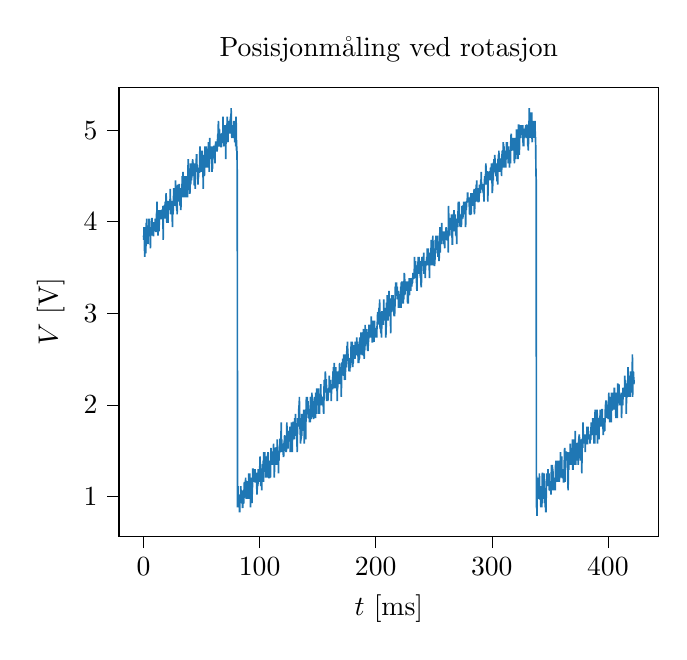
\begin{tikzpicture}

\definecolor{darkgray176}{RGB}{176,176,176}
\definecolor{steelblue31119180}{RGB}{31,119,180}

\begin{axis}[
tick align=outside,
tick pos=left,
title={Posisjonmåling ved rotasjon},
x grid style={darkgray176},
xlabel={\(\displaystyle t\) [ms]},
xmin=-21.12943, xmax=443.71803,
xtick style={color=black},
xtick={-100,0,100,200,300,400,500},
xticklabels={
  \(\displaystyle {\ensuremath{-}100}\),
  \(\displaystyle {0}\),
  \(\displaystyle {100}\),
  \(\displaystyle {200}\),
  \(\displaystyle {300}\),
  \(\displaystyle {400}\),
  \(\displaystyle {500}\)
},
y grid style={darkgray176},
ylabel={\(\displaystyle V\) [V]},
ymin=0.5644037625, ymax=5.4628464875,
ytick style={color=black},
ytick={0,1,2,3,4,5,6},
yticklabels={
  \(\displaystyle {0}\),
  \(\displaystyle {1}\),
  \(\displaystyle {2}\),
  \(\displaystyle {3}\),
  \(\displaystyle {4}\),
  \(\displaystyle {5}\),
  \(\displaystyle {6}\)
}
]
\addplot [semithick, steelblue31119180]
table {%
0 3.8485825
0.211400000000417 3.802194
0.422800000000834 3.9413595
0.634200000000362 3.8485825
0.845600000000779 3.7094265
1.05700000000031 3.6166495
1.26840000000072 3.9413595
1.47980000000025 3.802194
1.69120000000067 3.663038
1.9026000000002 3.663038
2.11400000000062 3.755815
2.32540000000014 3.987748
2.53680000000056 3.8485825
2.74820000000009 4.034127
2.95960000000051 3.894971
3.17100000000003 3.755815
3.38240000000045 3.8485825
3.59380000000087 3.802194
3.8052000000004 3.755815
4.01660000000081 3.8485825
4.22800000000034 3.8485825
4.43940000000076 3.8485825
4.65080000000029 4.034127
4.8622000000007 3.894971
5.07360000000023 3.894971
5.28500000000065 3.8485825
5.49640000000018 3.8485825
5.7078000000006 3.8485825
5.91920000000012 3.7094265
6.13060000000054 3.8485825
6.34200000000007 3.9413595
6.55340000000049 3.894971
6.76480000000002 4.034127
6.97620000000043 3.8485825
7.18760000000085 4.034127
7.39900000000038 4.034127
7.61040000000079 3.8485825
7.82180000000032 3.894971
8.03320000000074 3.894971
8.24460000000027 3.894971
8.45600000000069 3.8485825
8.66740000000021 3.8485825
8.87880000000063 3.987748
9.09020000000016 3.987748
9.30160000000058 3.894971
9.5130000000001 3.987748
9.72440000000052 3.9413595
9.93580000000005 3.9413595
10.1472000000005 4.034127
10.3586 3.987748
10.5700000000004 4.034127
10.7814000000008 3.894971
10.9928000000004 3.894971
11.2042000000008 4.0805155
11.4156000000003 4.0805155
11.6270000000007 4.219681
11.8384000000002 3.9413595
12.0498000000007 4.126904
12.2612000000002 4.034127
12.4726000000006 3.8485825
12.6840000000001 3.987748
12.8954000000006 3.987748
13.1068000000001 3.987748
13.3182000000005 3.894971
13.5296 3.987748
13.7410000000004 4.126904
13.9524000000009 4.034127
14.1638000000004 4.0805155
14.3752000000008 4.0805155
14.5866000000003 4.126904
14.7980000000008 4.0805155
15.0094000000003 4.034127
15.2208000000007 4.034127
15.4322000000002 4.034127
15.6436000000006 4.0805155
15.8550000000002 4.034127
16.0664000000006 4.126904
16.2778000000001 4.126904
16.4892000000005 4.034127
16.7006000000001 4.1732925
16.9120000000005 3.802194
17.1234 4.126904
17.3348000000004 4.034127
17.5462000000008 4.126904
17.7576000000004 4.0805155
17.9690000000008 4.1732925
18.1804000000003 4.1732925
18.3918000000007 4.034127
18.6032000000003 4.219681
18.8146000000007 4.126904
19.0260000000002 4.219681
19.2374000000006 4.1732925
19.4488000000002 4.3124485
19.6602000000006 4.1732925
19.8716000000001 4.1732925
20.0830000000005 3.987748
20.2944 4.0805155
20.5058000000005 4.126904
20.7172000000009 4.034127
20.9286000000004 4.1732925
21.1400000000008 3.987748
21.3514000000004 4.219681
21.5628000000008 4.219681
21.7742000000003 4.1732925
21.9856000000007 4.126904
22.1970000000002 4.1732925
22.4084000000007 4.219681
22.6198000000002 4.1732925
22.8312000000006 4.219681
23.0426000000001 4.358837
23.2540000000006 4.1732925
23.4654000000001 4.0805155
23.6768000000005 4.219681
23.8882 4.219681
24.0996000000004 4.219681
24.3110000000009 4.0805155
24.5224000000004 4.1732925
24.7338000000008 4.034127
24.9452000000003 3.9413595
25.1566000000008 4.126904
25.3680000000003 4.0805155
25.5794000000007 4.126904
25.7908000000002 4.219681
26.0022000000006 4.358837
26.2136000000002 4.358837
26.4250000000006 4.3124485
26.6364000000001 4.358837
26.8478000000005 4.26606
27.0592000000001 4.219681
27.2706000000005 4.1732925
27.482 4.451614
27.6934000000004 4.358837
27.9048000000008 4.26606
28.1162000000004 4.1732925
28.3276000000008 4.219681
28.5390000000003 4.126904
28.7504000000007 4.219681
28.9618000000003 4.0805155
29.1732000000007 4.358837
29.3846000000002 4.4052255
29.5960000000006 4.26606
29.8074000000002 4.219681
30.0188000000006 4.358837
30.2302000000001 4.3124485
30.4416000000005 4.219681
30.653 4.4052255
30.8644000000005 4.4052255
31.0758000000009 4.26606
31.2872000000004 4.3124485
31.4986000000008 4.1732925
31.7100000000003 4.358837
31.9214000000008 4.358837
32.1328000000003 4.126904
32.3442000000007 4.219681
32.5556000000002 4.358837
32.7670000000007 4.3124485
32.9784000000002 4.26606
33.1898000000006 4.4052255
33.4012000000001 4.4980025
33.6126000000005 4.4052255
33.8240000000001 4.26606
34.0354000000005 4.5443815
34.2468 4.358837
34.4582000000004 4.451614
34.6696000000009 4.4052255
34.8810000000004 4.358837
35.0924000000008 4.4980025
35.3038000000003 4.3124485
35.5152000000007 4.26606
35.7266000000003 4.4052255
35.9380000000007 4.4980025
36.1494000000002 4.26606
36.3608000000006 4.3124485
36.5722000000002 4.26606
36.7836000000006 4.4980025
36.9950000000001 4.358837
37.2064000000005 4.358837
37.4178000000001 4.358837
37.6292000000005 4.4052255
37.8406 4.26606
38.0520000000004 4.358837
38.2634000000008 4.5443815
38.4748000000004 4.683547
38.6862000000008 4.4980025
38.8976000000003 4.451614
39.1090000000007 4.451614
39.3204000000003 4.5443815
39.5318000000007 4.4052255
39.7432000000002 4.3124485
39.9546000000006 4.3124485
40.1660000000001 4.451614
40.3774000000006 4.6371585
40.5888000000001 4.4052255
40.8002000000005 4.5443815
41.0116 4.5443815
41.2230000000005 4.59077
41.4344000000009 4.451614
41.6458000000004 4.6371585
41.8572000000008 4.4980025
42.0686000000003 4.5443815
42.2800000000008 4.683547
42.4914000000003 4.6371585
42.7028000000007 4.6371585
42.9142000000002 4.59077
43.1256000000007 4.4980025
43.3370000000002 4.59077
43.5484000000006 4.59077
43.7598000000001 4.4052255
43.9712000000005 4.4052255
44.1826000000001 4.6371585
44.3940000000005 4.59077
44.6054 4.358837
44.8168000000004 4.59077
45.0282000000009 4.5443815
45.2396000000004 4.59077
45.4510000000008 4.683547
45.6624000000003 4.7299355
45.8738000000007 4.7299355
46.0852000000003 4.5443815
46.2966000000007 4.59077
46.5080000000002 4.5443815
46.7194000000006 4.59077
46.9308000000002 4.4052255
47.1422000000006 4.4980025
47.3536000000001 4.4980025
47.5650000000005 4.59077
47.7764000000001 4.5443815
47.9878000000005 4.5443815
48.1992 4.5443815
48.4106000000004 4.7299355
48.6220000000008 4.822703
48.8334000000004 4.59077
49.0448000000008 4.7299355
49.2562000000003 4.7299355
49.4676000000007 4.683547
49.6790000000003 4.59077
49.8904000000007 4.5443815
50.1018000000002 4.59077
50.3132000000006 4.7763145
50.5246000000001 4.5443815
50.7360000000006 4.59077
50.9474000000001 4.5443815
51.1588000000005 4.7299355
51.3702 4.358837
51.5816000000004 4.5443815
51.7930000000009 4.683547
52.0044000000004 4.7299355
52.2158000000008 4.6371585
52.4272000000003 4.4980025
52.6386000000008 4.59077
52.8500000000003 4.822703
53.0614000000007 4.59077
53.2728000000002 4.683547
53.4842000000006 4.683547
53.6956000000002 4.7299355
53.9070000000006 4.683547
54.1184000000001 4.822703
54.3298000000005 4.7299355
54.5412000000001 4.6371585
54.7526000000005 4.59077
54.964 4.6371585
55.1754000000004 4.59077
55.3868000000008 4.6371585
55.5982000000004 4.59077
55.8096000000008 4.683547
56.0210000000003 4.8690915
56.2324000000007 4.7299355
56.4438000000003 4.822703
56.6552000000007 4.5443815
56.8666000000002 4.7299355
57.0780000000006 4.91548
57.2894000000002 4.7299355
57.5008000000006 4.683547
57.7122000000001 4.7763145
57.9236000000005 4.822703
58.135 4.683547
58.3464000000005 4.822703
58.5578 4.7763145
58.7692000000004 4.822703
58.9806000000008 4.5443815
59.1920000000004 4.59077
59.4034000000008 4.59077
59.6148000000003 4.7299355
59.8262000000007 4.822703
60.0376000000002 4.7299355
60.2490000000007 4.7299355
60.4604000000002 4.7763145
60.6718000000006 4.822703
60.8832000000001 4.822703
61.0946000000006 4.7763145
61.3060000000001 4.7299355
61.5174000000005 4.6371585
61.7288 4.7763145
61.9402000000004 4.822703
62.1516000000009 4.8690915
62.3630000000004 4.8690915
62.5744000000008 4.8690915
62.7858000000003 4.7763145
62.9972000000008 4.7763145
63.2086000000003 4.7763145
63.4200000000007 4.7763145
63.6314000000002 4.8690915
63.8428000000006 4.91548
64.0542000000002 4.9618685
64.2656000000006 4.91548
64.4770000000001 5.1010245
64.6884000000005 5.054636
64.8998000000001 4.8690915
65.1112000000005 4.822703
65.3226 4.8690915
65.5340000000004 5.0082475
65.7454000000008 4.822703
65.9568000000004 4.91548
66.1682000000008 4.8690915
66.3796000000003 4.9618685
66.5910000000007 4.822703
66.8024000000003 4.822703
67.0138000000007 4.822703
67.2252000000002 4.91548
67.4366000000006 4.91548
67.6480000000002 4.9618685
67.8594000000006 4.9618685
68.0708000000001 4.91548
68.2822000000005 4.8690915
68.4936 5.147413
68.7050000000005 4.91548
68.9164000000009 4.8690915
69.1278000000004 4.822703
69.3392000000008 4.9618685
69.5506000000003 4.8690915
69.7620000000008 4.91548
69.9734000000003 5.054636
70.1848000000007 4.8690915
70.3962000000002 4.9618685
70.6076000000007 4.9618685
70.8190000000002 4.683547
71.0304000000006 4.91548
71.2418000000001 5.0082475
71.4532000000005 4.9618685
71.6646000000001 5.054636
71.8760000000005 5.0082475
72.0874 5.147413
72.2988000000004 4.9618685
72.5102000000009 4.91548
72.7216000000004 4.8690915
72.9330000000008 5.1010245
73.1444000000003 5.054636
73.3558000000008 4.9618685
73.5672000000003 5.054636
73.7786000000007 5.054636
73.9900000000002 4.9618685
74.2014000000006 5.054636
74.4128000000002 4.9618685
74.6242000000006 5.054636
74.8356000000001 5.147413
75.0470000000005 5.0082475
75.2584000000001 5.0082475
75.4698000000005 5.24019
75.6812 5.0082475
75.8926000000004 4.9618685
76.1040000000008 4.91548
76.3154000000004 5.054636
76.5268000000008 4.9618685
76.7382000000003 5.054636
76.9496000000007 4.91548
77.1610000000003 4.9618685
77.3724000000007 5.0082475
77.5838000000002 5.0082475
77.7952000000006 5.1010245
78.0066000000001 5.054636
78.2180000000006 4.9618685
78.4294000000001 4.91548
78.6408000000005 4.8690915
78.8522 5.054636
79.0636000000005 4.8690915
79.2750000000009 5.1010245
79.4864000000004 4.822703
79.6978000000008 5.147413
79.9092000000003 5.0082475
80.1206000000008 4.7763145
80.3320000000003 4.822703
80.5434000000007 4.7299355
80.7548000000002 4.451614
80.9662000000007 0.8798344
81.1776000000002 1.0653808
81.3890000000006 1.1117674
81.6004000000001 0.9726076
81.8118000000005 0.9726076
82.0232000000001 0.926221
82.2346000000005 0.9726076
82.446 0.9726076
82.6574000000004 0.83344685
82.8688000000008 0.83344685
83.0802000000004 1.0189942
83.2916000000008 0.9726076
83.5030000000003 0.926221
83.7144000000008 1.1117674
83.9258000000003 1.0653808
84.1372000000007 1.0189942
84.3486000000002 0.926221
84.5600000000006 0.9726076
84.7714000000002 0.9726076
84.9828000000006 0.9726076
85.1942000000001 0.8798344
85.4056000000005 0.8798344
85.617 1.0653808
85.8284000000005 0.926221
86.0398 0.926221
86.2512000000004 0.926221
86.4626000000008 0.9726076
86.6740000000004 1.1117674
86.8854000000008 1.158154
87.0968000000003 1.1117674
87.3082000000007 1.158154
87.5196000000003 1.1117674
87.7310000000007 1.0653808
87.9424000000002 1.2045406
88.1538000000006 1.0653808
88.3652000000001 0.9726076
88.5766000000006 1.1117674
88.7880000000001 1.1117674
88.9994000000005 1.158154
89.2108 1.158154
89.4222000000005 1.0653808
89.6336000000009 1.1117674
89.8450000000004 1.0653808
90.0564000000008 0.9726076
90.2678000000003 1.1117674
90.4792000000008 1.0189942
90.6906000000003 1.250931
90.9020000000007 1.1117674
91.1134000000002 1.0189942
91.3248000000006 0.9726076
91.5362000000002 1.250931
91.7476000000006 1.0189942
91.9590000000001 1.1117674
92.1704000000005 0.8798344
92.3818000000001 1.2045406
92.5932000000005 1.158154
92.8046 1.0653808
93.0160000000004 1.1117674
93.2274000000008 1.0189942
93.4388000000004 0.926221
93.6502000000008 1.0653808
93.8616000000003 1.1117674
94.0730000000007 1.29731
94.2844000000003 1.29731
94.4958000000007 1.2045406
94.7072000000002 1.250931
94.9186000000006 1.2045406
95.1300000000002 1.29731
95.3414000000006 1.158154
95.5528000000001 1.2045406
95.7642000000005 1.2045406
95.9756 1.29731
96.1870000000005 1.158154
96.3984 1.158154
96.6098000000004 1.2045406
96.8212000000008 1.2045406
97.0326000000004 1.250931
97.2440000000008 1.250931
97.4554000000003 1.2045406
97.6668000000007 1.0189942
97.8782000000002 1.0653808
98.0896000000007 1.2045406
98.3010000000002 1.250931
98.5124000000006 1.1117674
98.7238000000001 1.29731
98.9352000000005 1.158154
99.1466000000001 1.2045406
99.3580000000005 1.158154
99.5694 1.250931
99.7808000000005 1.2045406
99.9922000000009 1.2045406
100.2036 1.3436985
100.415000000001 1.4364755
100.6264 1.2045406
100.837800000001 1.250931
101.0492 1.1117674
101.260600000001 1.158154
101.472 1.158154
101.683400000001 1.158154
101.8948 1.0653808
102.106200000001 1.29731
102.3176 1.29731
102.529000000001 1.3436985
102.7404 1.3436985
102.9518 1.29731
103.1632 1.390087
103.3746 1.158154
103.586000000001 1.482864
103.7974 1.3436985
104.008800000001 1.29731
104.2202 1.3436985
104.431600000001 1.482864
104.643 1.3436985
104.854400000001 1.29731
105.0658 1.29731
105.277200000001 1.2045406
105.4886 1.4364755
105.700000000001 1.2045406
105.9114 1.29731
106.122800000001 1.3436985
106.3342 1.3436985
106.5456 1.2045406
106.757000000001 1.4364755
106.9684 1.4364755
107.179800000001 1.482864
107.3912 1.29731
107.602600000001 1.29731
107.814 1.3436985
108.025400000001 1.2045406
108.2368 1.2045406
108.448200000001 1.2045406
108.6596 1.390087
108.871000000001 1.2045406
109.0824 1.3436985
109.293800000001 1.2045406
109.5052 1.3436985
109.7166 1.5292525
109.928 1.482864
110.1394 1.482864
110.350800000001 1.3436985
110.5622 1.482864
110.773600000001 1.482864
110.985 1.4364755
111.196400000001 1.4364755
111.4078 1.3436985
111.619200000001 1.482864
111.8306 1.4364755
112.042000000001 1.5756315
112.2534 1.4364755
112.464800000001 1.3436985
112.6762 1.2045406
112.887600000001 1.390087
113.099 1.482864
113.3104 1.3436985
113.5218 1.390087
113.7332 1.482864
113.944600000001 1.5292525
114.156 1.4364755
114.367400000001 1.5292525
114.5788 1.5292525
114.790200000001 1.3436985
115.0016 1.390087
115.213000000001 1.62202
115.4244 1.482864
115.635800000001 1.482864
115.8472 1.4364755
116.058600000001 1.4364755
116.27 1.250931
116.481400000001 1.482864
116.6928 1.390087
116.9042 1.482864
117.115600000001 1.482864
117.327 1.5292525
117.538400000001 1.62202
117.7498 1.62202
117.961200000001 1.5292525
118.1726 1.62202
118.384000000001 1.62202
118.5954 1.8075645
118.806800000001 1.482864
119.0182 1.62202
119.229600000001 1.5292525
119.441 1.5292525
119.652400000001 1.5292525
119.8638 1.5756315
120.0752 1.5292525
120.2866 1.482864
120.498 1.4364755
120.709400000001 1.4364755
120.9208 1.5756315
121.132200000001 1.5756315
121.3436 1.62202
121.555000000001 1.6684085
121.7664 1.5756315
121.977800000001 1.5756315
122.1892 1.62202
122.400600000001 1.5756315
122.612 1.482864
122.823400000001 1.62202
123.0348 1.482864
123.246200000001 1.5756315
123.4576 1.8075645
123.669 1.6684085
123.8804 1.5292525
124.0918 1.5292525
124.303200000001 1.5292525
124.5146 1.5292525
124.726000000001 1.714797
124.9374 1.62202
125.148800000001 1.714797
125.3602 1.62202
125.571600000001 1.714797
125.783 1.6684085
125.994400000001 1.714797
126.2058 1.7611855
126.417200000001 1.482864
126.6286 1.714797
126.840000000001 1.62202
127.0514 1.6684085
127.2628 1.6684085
127.474200000001 1.8075645
127.6856 1.6684085
127.897000000001 1.6684085
128.1084 1.482864
128.319800000001 1.6684085
128.5312 1.6684085
128.742600000001 1.714797
128.954 1.8075645
129.165400000001 1.8075645
129.3768 1.8075645
129.588200000001 1.8075645
129.7996 1.62202
130.011000000001 1.7611855
130.2224 1.853953
130.4338 1.6684085
130.6452 1.6684085
130.8566 1.9003415
131.068000000001 1.6684085
131.2794 1.6684085
131.490800000001 1.6684085
131.7022 1.7611855
131.913600000001 1.62202
132.125 1.6684085
132.336400000001 1.482864
132.5478 1.6684085
132.759200000001 1.853953
132.9706 1.8075645
133.182000000001 1.7611855
133.3934 1.8075645
133.604800000001 1.8075645
133.8162 1.9931185
134.0276 1.8075645
134.239 2.085886
134.4504 1.853953
134.661800000001 1.9003415
134.8732 1.714797
135.084600000001 1.6684085
135.296 1.5756315
135.507400000001 1.6684085
135.7188 1.62202
135.930200000001 1.6684085
136.1416 1.6684085
136.353000000001 1.6684085
136.5644 1.9003415
136.775800000001 1.853953
136.9872 1.853953
137.198600000001 1.853953
137.41 1.853953
137.6214 1.8075645
137.832800000001 1.714797
138.0442 1.94673
138.255600000001 1.853953
138.467 1.5756315
138.678400000001 1.8075645
138.8898 1.94673
139.101200000001 1.7611855
139.3126 1.7611855
139.524000000001 1.7611855
139.7354 1.62202
139.946800000001 1.9003415
140.1582 2.0394975
140.369600000001 2.085886
140.581 1.853953
140.7924 1.9931185
141.0038 2.085886
141.2152 1.94673
141.426600000001 1.9931185
141.638 2.0394975
141.849400000001 1.9003415
142.0608 1.94673
142.272200000001 1.94673
142.4836 1.853953
142.695000000001 1.9003415
142.9064 1.8075645
143.117800000001 1.9003415
143.3292 1.94673
143.540600000001 1.8075645
143.752 2.085886
143.963400000001 1.9003415
144.1748 1.853953
144.3862 1.853953
144.597600000001 1.94673
144.809 1.9931185
145.020400000001 2.1322745
145.2318 1.9931185
145.443200000001 1.9931185
145.6546 2.085886
145.866000000001 1.9931185
146.0774 1.94673
146.288800000001 1.853953
146.5002 1.853953
146.711600000001 2.0394975
146.923 1.9003415
147.134400000001 1.853953
147.3458 1.9003415
147.557200000001 1.853953
147.7686 2.085886
147.98 2.0394975
148.191400000001 1.853953
148.4028 2.1322745
148.614200000001 1.94673
148.8256 1.9931185
149.037000000001 1.9003415
149.2484 2.178663
149.459800000001 2.085886
149.6712 1.9931185
149.882600000001 2.1322745
150.094 1.9931185
150.305400000001 2.178663
150.5168 1.9931185
150.728200000001 2.085886
150.9396 1.9003415
151.151 1.94673
151.3624 1.94673
151.5738 1.9003415
151.785200000001 2.0394975
151.9966 2.085886
152.208000000001 2.178663
152.4194 1.9931185
152.630800000001 2.2250515
152.8422 2.085886
153.053600000001 2.085886
153.265 2.085886
153.476400000001 2.0394975
153.6878 2.0394975
153.899200000001 1.9931185
154.1106 2.0394975
154.322000000001 2.085886
154.5334 2.0394975
154.7448 2.0394975
154.956200000001 1.94673
155.1676 1.9003415
155.379000000001 2.0394975
155.5904 2.27144
155.801800000001 2.1322745
156.0132 2.178663
156.224600000001 2.1322745
156.436 2.317819
156.647400000001 2.3642075
156.8588 2.2250515
157.070200000001 2.178663
157.2816 2.27144
157.493000000001 2.27144
157.7044 2.0394975
157.915800000001 2.178663
158.1272 2.0394975
158.3386 2.178663
158.550000000001 2.085886
158.7614 2.0394975
158.972800000001 2.085886
159.1842 2.1322745
159.395600000001 2.178663
159.607 2.1322745
159.818400000001 2.178663
160.0298 2.317819
160.241200000001 2.178663
160.4526 2.1322745
160.664000000001 2.27144
160.8754 2.178663
161.086800000001 2.27144
161.2982 2.178663
161.5096 2.2250515
161.721 2.0394975
161.9324 2.178663
162.143800000001 2.178663
162.3552 2.178663
162.566600000001 2.178663
162.778 2.178663
162.989400000001 2.27144
163.2008 2.3642075
163.412200000001 2.178663
163.6236 2.410596
163.835000000001 2.317819
164.0464 2.27144
164.257800000001 2.4569845
164.4692 2.3642075
164.680600000001 2.178663
164.892 2.410596
165.1034 2.2250515
165.314800000001 2.317819
165.5262 2.410596
165.737600000001 2.27144
165.949 2.317819
166.160400000001 2.178663
166.3718 2.27144
166.583200000001 2.3642075
166.7946 2.0394975
167.006000000001 2.178663
167.2174 2.178663
167.428800000001 2.3642075
167.6402 2.317819
167.851600000001 2.2250515
168.063 2.317819
168.2744 2.317819
168.4858 2.3642075
168.6972 2.3642075
168.908600000001 2.4569845
169.12 2.410596
169.331400000001 2.2250515
169.5428 2.317819
169.754200000001 2.3642075
169.9656 2.2250515
170.177000000001 2.27144
170.3884 2.085886
170.599800000001 2.3642075
170.8112 2.410596
171.022600000001 2.4569845
171.234 2.4569845
171.445400000001 2.317819
171.6568 2.503373
171.8682 2.4569845
172.0796 2.317819
172.291 2.3642075
172.502400000001 2.549752
172.7138 2.4569845
172.925200000001 2.4569845
173.1366 2.27144
173.348000000001 2.549752
173.5594 2.317819
173.770800000001 2.27144
173.9822 2.410596
174.193600000001 2.549752
174.405 2.4569845
174.616400000001 2.410596
174.8278 2.4569845
175.039200000001 2.549752
175.2506 2.642529
175.462 2.503373
175.673400000001 2.6889175
175.8848 2.5961405
176.096200000001 2.549752
176.3076 2.503373
176.519000000001 2.503373
176.7304 2.4569845
176.941800000001 2.3642075
177.1532 2.503373
177.364600000001 2.503373
177.576 2.3642075
177.787400000001 2.410596
177.9988 2.410596
178.210200000001 2.410596
178.4216 2.503373
178.633 2.503373
178.8444 2.6889175
179.0558 2.4569845
179.267200000001 2.642529
179.4786 2.549752
179.690000000001 2.6889175
179.9014 2.642529
180.112800000001 2.549752
180.3242 2.410596
180.535600000001 2.5961405
180.747 2.4569845
180.958400000001 2.642529
181.1698 2.642529
181.381200000001 2.549752
181.5926 2.5961405
181.804000000001 2.503373
182.0154 2.642529
182.2268 2.503373
182.4382 2.6889175
182.6496 2.5961405
182.861000000001 2.549752
183.0724 2.549752
183.283800000001 2.549752
183.4952 2.549752
183.706600000001 2.735306
183.918 2.549752
184.129400000001 2.5961405
184.3408 2.6889175
184.552200000001 2.642529
184.7636 2.549752
184.975000000001 2.4569845
185.1864 2.549752
185.397800000001 2.4569845
185.6092 2.503373
185.8206 2.5961405
186.032000000001 2.503373
186.2434 2.735306
186.454800000001 2.549752
186.6662 2.642529
186.877600000001 2.642529
187.089 2.549752
187.300400000001 2.781685
187.5118 2.781685
187.723200000001 2.642529
187.9346 2.5961405
188.146000000001 2.6889175
188.3574 2.781685
188.568800000001 2.549752
188.7802 2.549752
188.9916 2.6889175
189.203 2.735306
189.4144 2.8280735
189.625800000001 2.6889175
189.8372 2.5961405
190.048600000001 2.503373
190.26 2.5961405
190.471400000001 2.5961405
190.6828 2.642529
190.894200000001 2.874462
191.1056 2.642529
191.317000000001 2.781685
191.5284 2.6889175
191.739800000001 2.781685
191.9512 2.735306
192.162600000001 2.6889175
192.374 2.8280735
192.5854 2.6889175
192.796800000001 2.6889175
193.0082 2.5961405
193.219600000001 2.5961405
193.431 2.5961405
193.642400000001 2.735306
193.8538 2.6889175
194.065200000001 2.781685
194.2766 2.874462
194.488000000001 2.781685
194.6994 2.8280735
194.910800000001 2.874462
195.1222 2.8280735
195.333600000001 2.874462
195.545 2.735306
195.7564 2.8280735
195.9678 2.735306
196.1792 2.967239
196.390600000001 2.8280735
196.602 2.874462
196.813400000001 2.781685
197.0248 2.6889175
197.236200000001 2.6889175
197.4476 2.781685
197.659000000001 2.8280735
197.8704 2.9208505
198.081800000001 2.8280735
198.2932 2.874462
198.504600000001 2.6889175
198.716 2.781685
198.927400000001 2.9208505
199.1388 2.8280735
199.3502 2.8280735
199.5616 2.8280735
199.773 2.735306
199.984400000001 2.781685
200.1958 2.8280735
200.407200000001 2.8280735
200.6186 2.781685
200.830000000001 2.735306
201.0414 2.8280735
201.252800000001 2.874462
201.4642 2.9208505
201.675600000001 3.0136275
201.887 2.9208505
202.098400000001 2.967239
202.3098 2.967239
202.521200000001 2.9208505
202.7326 3.0600065
202.944 2.9208505
203.155400000001 2.874462
203.3668 3.1527835
203.578200000001 2.967239
203.7896 2.8280735
204.001000000001 2.874462
204.2124 2.9208505
204.423800000001 2.781685
204.6352 2.9208505
204.846600000001 2.9208505
205.058 2.735306
205.269400000001 3.0136275
205.4808 3.0136275
205.692200000001 2.967239
205.9036 2.9208505
206.115 3.0136275
206.3264 2.9208505
206.5378 2.874462
206.749200000001 2.967239
206.9606 3.1527835
207.172000000001 2.967239
207.3834 2.9208505
207.594800000001 2.967239
207.8062 2.9208505
208.017600000001 2.967239
208.229 3.0600065
208.440400000001 3.0136275
208.6518 2.735306
208.863200000001 2.781685
209.0746 2.874462
209.286000000001 3.106395
209.4974 3.106395
209.7088 3.0600065
209.9202 3.199172
210.1316 3.0136275
210.343000000001 3.1527835
210.5544 2.9208505
210.765800000001 3.0600065
210.9772 3.106395
211.188600000001 3.0136275
211.4 3.2455605
211.611400000001 3.0136275
211.8228 3.0600065
212.034200000001 2.967239
212.2456 3.106395
212.457000000001 2.967239
212.6684 3.0136275
212.879800000001 2.781685
213.0912 3.1527835
213.3026 3.1527835
213.514000000001 3.0136275
213.7254 3.199172
213.936800000001 3.106395
214.1482 3.0600065
214.359600000001 3.199172
214.571 3.0600065
214.782400000001 3.0600065
214.9938 3.199172
215.205200000001 3.0136275
215.4166 3.0600065
215.628000000001 3.106395
215.8394 2.967239
216.050800000001 3.0600065
216.2622 2.967239
216.4736 3.0600065
216.685 3.106395
216.8964 3.2919395
217.107800000001 3.1527835
217.3192 3.338328
217.530600000001 3.199172
217.742 3.199172
217.953400000001 3.338328
218.1648 3.199172
218.376200000001 3.199172
218.5876 3.2919395
218.799000000001 3.199172
219.0104 3.1527835
219.221800000001 3.199172
219.4332 3.2455605
219.644600000001 3.0600065
219.856 3.199172
220.0674 3.0600065
220.2788 3.1527835
220.4902 3.106395
220.701600000001 3.1527835
220.913 3.199172
221.124400000001 3.199172
221.3358 3.199172
221.547200000001 3.2919395
221.7586 3.0600065
221.970000000001 3.338328
222.1814 3.2919395
222.392800000001 3.106395
222.6042 3.338328
222.815600000001 3.338328
223.027 3.199172
223.2384 3.199172
223.4498 3.2919395
223.6612 3.106395
223.872600000001 3.199172
224.084 3.1527835
224.295400000001 3.199172
224.5068 3.431105
224.718200000001 3.431105
224.9296 3.3847165
225.141000000001 3.199172
225.3524 3.338328
225.563800000001 3.338328
225.7752 3.338328
225.986600000001 3.338328
226.198 3.338328
226.409400000001 3.338328
226.6208 3.2455605
226.8322 3.338328
227.0436 3.338328
227.255 3.338328
227.466400000001 3.106395
227.6778 3.2455605
227.889200000001 3.338328
228.1006 3.106395
228.312000000001 3.338328
228.5234 3.338328
228.734800000001 3.2919395
228.9462 3.3847165
229.157600000001 3.199172
229.369 3.338328
229.580400000001 3.338328
229.7918 3.3847165
230.003200000001 3.338328
230.2146 3.2455605
230.426 3.338328
230.637400000001 3.338328
230.8488 3.3847165
231.060200000001 3.2919395
231.2716 3.338328
231.483000000001 3.338328
231.6944 3.338328
231.905800000001 3.3847165
232.1172 3.431105
232.328600000001 3.431105
232.54 3.3847165
232.751400000001 3.3847165
232.9628 3.431105
233.174200000001 3.3847165
233.3856 3.6166495
233.597 3.3847165
233.8084 3.5238725
234.0198 3.431105
234.231200000001 3.570261
234.4426 3.5238725
234.654000000001 3.4774935
234.8654 3.4774935
235.076800000001 3.3847165
235.2882 3.2919395
235.499600000001 3.2455605
235.711 3.3847165
235.922400000001 3.431105
236.1338 3.5238725
236.345200000001 3.431105
236.5566 3.6166495
236.768000000001 3.431105
236.9794 3.570261
237.1908 3.4774935
237.4022 3.6166495
237.6136 3.431105
237.825000000001 3.4774935
238.0364 3.431105
238.247800000001 3.570261
238.4592 3.3847165
238.670600000001 3.5238725
238.882 3.4774935
239.093400000001 3.2919395
239.3048 3.2919395
239.516200000001 3.431105
239.7276 3.5238725
239.939000000001 3.6166495
240.1504 3.5238725
240.361800000001 3.5238725
240.5732 3.570261
240.7846 3.6166495
240.996000000001 3.570261
241.2074 3.6166495
241.418800000001 3.663038
241.6302 3.431105
241.841600000001 3.570261
242.053 3.5238725
242.264400000001 3.5238725
242.4758 3.570261
242.687200000001 3.3847165
242.8986 3.5238725
243.110000000001 3.5238725
243.3214 3.570261
243.532800000001 3.5238725
243.7442 3.570261
243.9556 3.6166495
244.167 3.5238725
244.3784 3.7094265
244.589800000001 3.570261
244.8012 3.6166495
245.012600000001 3.570261
245.224 3.7094265
245.435400000001 3.570261
245.6468 3.5238725
245.858200000001 3.570261
246.0696 3.570261
246.281000000001 3.3847165
246.4924 3.663038
246.703800000001 3.5238725
246.9152 3.570261
247.126600000001 3.5238725
247.338 3.570261
247.5494 3.5238725
247.7608 3.802194
247.9722 3.6166495
248.183600000001 3.7094265
248.395 3.5238725
248.606400000001 3.755815
248.8178 3.755815
249.029200000001 3.755815
249.2406 3.8485825
249.452000000001 3.5238725
249.6634 3.663038
249.874800000001 3.663038
250.0862 3.7094265
250.297600000001 3.663038
250.509 3.5238725
250.7204 3.5238725
250.9318 3.570261
251.1432 3.6166495
251.354600000001 3.802194
251.566 3.663038
251.777400000001 3.663038
251.9888 3.8485825
252.200200000001 3.7094265
252.4116 3.755815
252.623000000001 3.7094265
252.8344 3.7094265
253.045800000001 3.802194
253.2572 3.8485825
253.468600000001 3.7094265
253.68 3.6166495
253.891400000001 3.755815
254.1028 3.663038
254.3142 3.663038
254.5256 3.570261
254.737 3.6166495
254.948400000001 3.755815
255.1598 3.8485825
255.371200000001 3.9413595
255.5826 3.663038
255.794000000001 3.8485825
256.0054 3.8485825
256.216800000001 3.755815
256.4282 3.8485825
256.639600000001 3.8485825
256.851 3.987748
257.062400000001 3.802194
257.2738 3.8485825
257.485200000001 3.802194
257.6966 3.894971
257.908 3.8485825
258.1194 3.755815
258.3308 3.802194
258.542200000001 3.894971
258.7536 3.755815
258.965000000001 3.802194
259.1764 3.802194
259.387800000001 3.7094265
259.5992 3.802194
259.810600000001 3.8485825
260.022 3.894971
260.233400000001 3.802194
260.4448 3.894971
260.656200000001 3.9413595
260.8676 3.894971
261.079000000001 3.894971
261.2904 3.8485825
261.5018 3.802194
261.713200000001 3.802194
261.9246 3.894971
262.136000000001 3.802194
262.3474 3.8485825
262.558800000001 3.663038
262.7702 4.1732925
262.981600000001 3.9413595
263.193 4.034127
263.404400000001 3.987748
263.6158 3.894971
263.827200000001 3.8485825
264.0386 3.987748
264.250000000001 4.034127
264.4614 4.034127
264.672800000001 3.9413595
264.8842 3.9413595
265.0956 3.987748
265.307000000001 4.0805155
265.5184 3.9413595
265.729800000001 3.8485825
265.9412 3.755815
266.152600000001 3.755815
266.364 4.0805155
266.575400000001 3.987748
266.7868 4.034127
266.998200000001 3.894971
267.2096 4.0805155
267.421000000001 4.126904
267.6324 4.034127
267.8438 4.034127
268.0552 4.034127
268.2666 3.987748
268.478 4.0805155
268.6894 3.9413595
268.900800000001 3.8485825
269.1122 3.9413595
269.323600000001 4.034127
269.535 3.9413595
269.746400000001 3.755815
269.9578 3.987748
270.169200000001 3.987748
270.3806 3.987748
270.592000000001 3.9413595
270.8034 3.987748
271.014800000001 4.1732925
271.2262 4.219681
271.4376 4.034127
271.649 3.987748
271.8604 4.219681
272.071800000001 4.0805155
272.2832 4.0805155
272.494600000001 4.034127
272.706 3.9413595
272.917400000001 3.987748
273.1288 4.034127
273.340200000001 4.034127
273.5516 4.0805155
273.763000000001 3.9413595
273.9744 4.034127
274.185800000001 4.034127
274.3972 4.1732925
274.608600000001 4.0805155
274.82 4.126904
275.0314 4.034127
275.2428 4.0805155
275.4542 4.1732925
275.665600000001 4.1732925
275.877 4.219681
276.088400000001 4.126904
276.2998 4.1732925
276.511200000001 4.0805155
276.7226 4.219681
276.934000000001 4.126904
277.1454 4.219681
277.356800000001 3.9413595
277.5682 3.987748
277.779600000001 4.219681
277.991 4.126904
278.202400000001 4.1732925
278.4138 4.219681
278.6252 4.219681
278.836600000001 4.219681
279.048 4.3124485
279.259400000001 4.3124485
279.4708 4.219681
279.682200000001 4.219681
279.8936 4.26606
280.105000000001 4.219681
280.3164 4.219681
280.527800000001 4.26606
280.7392 4.0805155
280.950600000001 4.219681
281.162 4.219681
281.373400000001 4.0805155
281.5848 4.0805155
281.796200000001 4.219681
282.0076 4.3124485
282.219 4.0805155
282.430400000001 4.219681
282.6418 4.219681
282.853200000001 4.3124485
283.0646 4.219681
283.276000000001 4.219681
283.4874 4.219681
283.698800000001 4.1732925
283.9102 4.26606
284.121600000001 4.3124485
284.333 4.26606
284.544400000001 4.219681
284.7558 4.358837
284.967200000001 4.0805155
285.1786 4.126904
285.39 4.1732925
285.6014 4.3124485
285.8128 4.26606
286.024200000001 4.3124485
286.2356 4.358837
286.447000000001 4.358837
286.6584 4.4052255
286.869800000001 4.26606
287.0812 4.451614
287.292600000001 4.219681
287.504 4.26606
287.715400000001 4.26606
287.9268 4.358837
288.138200000001 4.358837
288.3496 4.219681
288.561 4.219681
288.7724 4.358837
288.9838 4.219681
289.195200000001 4.3124485
289.4066 4.4052255
289.618000000001 4.358837
289.8294 4.4052255
290.040800000001 4.358837
290.2522 4.3124485
290.463600000001 4.451614
290.675 4.4052255
290.886400000001 4.5443815
291.0978 4.4052255
291.309200000001 4.358837
291.5206 4.358837
291.732000000001 4.4052255
291.9434 4.4052255
292.1548 4.358837
292.3662 4.358837
292.5776 4.3124485
292.789000000001 4.358837
293.0004 4.358837
293.211800000001 4.219681
293.4232 4.4052255
293.634600000001 4.4052255
293.846 4.4980025
294.057400000001 4.4052255
294.2688 4.4980025
294.480200000001 4.451614
294.6916 4.5443815
294.903000000001 4.6371585
295.1144 4.451614
295.325800000001 4.4052255
295.5372 4.5443815
295.7486 4.4980025
295.96 4.5443815
296.1714 4.5443815
296.382800000001 4.451614
296.5942 4.219681
296.805600000001 4.451614
297.017 4.5443815
297.228400000001 4.451614
297.4398 4.4980025
297.651200000001 4.451614
297.8626 4.4980025
298.074000000001 4.5443815
298.2854 4.5443815
298.496800000001 4.5443815
298.7082 4.4980025
298.919600000001 4.59077
299.131 4.4980025
299.3424 4.451614
299.553800000001 4.59077
299.7652 4.6371585
299.976600000001 4.4980025
300.188 4.451614
300.399400000001 4.3124485
300.6108 4.358837
300.822200000001 4.4052255
301.0336 4.5443815
301.245000000001 4.451614
301.4564 4.6371585
301.667800000001 4.6371585
301.8792 4.683547
302.090600000001 4.5443815
302.302 4.6371585
302.513400000001 4.7299355
302.7248 4.683547
302.9362 4.6371585
303.147600000001 4.5443815
303.359 4.5443815
303.570400000001 4.4980025
303.7818 4.5443815
303.993200000001 4.6371585
304.2046 4.5443815
304.416000000001 4.451614
304.6274 4.451614
304.838800000001 4.59077
305.0502 4.4052255
305.261600000001 4.683547
305.473 4.59077
305.684400000001 4.7299355
305.8958 4.6371585
306.1072 4.7763145
306.3186 4.5443815
306.53 4.59077
306.741400000001 4.59077
306.9528 4.5443815
307.164200000001 4.59077
307.3756 4.683547
307.587000000001 4.683547
307.7984 4.59077
308.009800000001 4.6371585
308.2212 4.683547
308.432600000001 4.4980025
308.644 4.7299355
308.855400000001 4.7299355
309.0668 4.7763145
309.2782 4.7299355
309.4896 4.683547
309.701 4.7763145
309.912400000001 4.8690915
310.1238 4.822703
310.335200000001 4.59077
310.5466 4.822703
310.758000000001 4.7299355
310.9694 4.7299355
311.180800000001 4.7299355
311.3922 4.7299355
311.603600000001 4.683547
311.815 4.7763145
312.026400000001 4.59077
312.2378 4.7299355
312.449200000001 4.683547
312.6606 4.8690915
312.872 4.7299355
313.0834 4.822703
313.2948 4.8690915
313.506200000001 4.7299355
313.7176 4.7763145
313.929000000001 4.822703
314.1404 4.6371585
314.351800000001 4.7299355
314.5632 4.7763145
314.774600000001 4.7763145
314.986 4.7299355
315.197400000001 4.59077
315.4088 4.7299355
315.620200000001 4.7299355
315.8316 4.822703
316.043000000001 4.6371585
316.2544 4.822703
316.4658 4.91548
316.677200000001 4.9618685
316.8886 4.8690915
317.100000000001 4.8690915
317.3114 4.91548
317.522800000001 4.822703
317.7342 4.7763145
317.945600000001 4.8690915
318.157 4.822703
318.368400000001 4.8690915
318.5798 4.91548
318.791200000001 4.822703
319.0026 4.8690915
319.214000000001 4.91548
319.4254 4.6371585
319.636800000001 4.683547
319.8482 4.8690915
320.0596 4.7763145
320.271000000001 4.7299355
320.4824 4.7763145
320.693800000001 4.683547
320.9052 4.91548
321.116600000001 4.7299355
321.328 5.0082475
321.539400000001 4.9618685
321.7508 4.91548
321.962200000001 4.7763145
322.1736 4.91548
322.385000000001 4.9618685
322.5964 4.683547
322.807800000001 4.7763145
323.0192 5.054636
323.2306 5.054636
323.442 4.7763145
323.6534 4.7299355
323.864800000001 4.822703
324.0762 5.054636
324.287600000001 4.9618685
324.499 4.9618685
324.710400000001 5.0082475
324.9218 4.91548
325.133200000001 4.9618685
325.3446 5.054636
325.556000000001 5.0082475
325.7674 5.0082475
325.978800000001 4.9618685
326.1902 4.9618685
326.4016 5.0082475
326.613 5.054636
326.8244 4.91548
327.035800000001 4.822703
327.2472 4.91548
327.458600000001 4.822703
327.67 4.9618685
327.881400000001 4.91548
328.0928 4.9618685
328.304200000001 5.0082475
328.5156 5.0082475
328.727000000001 4.9618685
328.9384 4.9618685
329.149800000001 5.054636
329.3612 5.0082475
329.572600000001 4.9618685
329.784 4.91548
329.9954 5.054636
330.2068 5.054636
330.4182 5.0082475
330.629600000001 5.054636
330.841 4.9618685
331.052400000001 4.822703
331.2638 4.91548
331.475200000001 4.7763145
331.6866 5.0082475
331.898000000001 5.0082475
332.1094 5.1010245
332.320800000001 5.24019
332.5322 5.1010245
332.743600000001 5.1010245
332.955 4.91548
333.166400000001 5.1010245
333.3778 5.054636
333.5892 5.1010245
333.8006 5.1938015
334.012 5.1010245
334.223400000001 5.1010245
334.4348 5.1938015
334.646200000001 4.91548
334.8576 4.8690915
335.069000000001 4.9618685
335.2804 5.1010245
335.491800000001 5.054636
335.7032 5.1010245
335.914600000001 4.91548
336.126 5.0082475
336.337400000001 5.054636
336.5488 5.054636
336.760200000001 5.1010245
336.9716 4.9618685
337.183 5.1010245
337.394400000001 4.9618685
337.6058 4.91548
337.817200000001 4.822703
338.0286 4.5443815
338.240000000001 4.451614
338.4514 0.8798344
338.662800000001 0.9726076
338.8742 0.78706025
339.085600000001 0.9726076
339.297 1.0653808
339.508400000001 1.1117674
339.7198 0.9726076
339.931200000001 1.2045406
340.1426 1.0653808
340.354 0.9726076
340.5654 1.1117674
340.7768 0.9726076
340.988200000001 1.250931
341.1996 1.0189942
341.411000000001 0.9726076
341.6224 0.9726076
341.833800000001 1.1117674
342.0452 0.9726076
342.256600000001 0.8798344
342.468 1.1117674
342.679400000001 0.9726076
342.8908 1.1117674
343.102200000001 0.8798344
343.3136 1.0189942
343.525000000001 1.250931
343.7364 1.250931
343.9478 1.0653808
344.1592 0.9726076
344.3706 1.0653808
344.582000000001 1.0653808
344.7934 1.158154
345.004800000001 0.9726076
345.2162 1.250931
345.427600000001 0.926221
345.639 0.9726076
345.850400000001 0.9726076
346.0618 0.8798344
346.273200000001 1.0653808
346.4846 0.83344685
346.696000000001 0.83344685
346.9074 1.0653808
347.118800000001 1.158154
347.3302 1.158154
347.5416 1.250931
347.753000000001 1.158154
347.9644 1.1117674
348.175800000001 1.158154
348.3872 1.29731
348.598600000001 1.1117674
348.81 1.158154
349.021400000001 1.158154
349.2328 1.250931
349.444200000001 1.0653808
349.6556 1.1117674
349.867000000001 1.158154
350.0784 1.158154
350.289800000001 1.0653808
350.5012 1.0653808
350.7126 1.158154
350.924 1.0189942
351.1354 1.1117674
351.346800000001 1.3436985
351.5582 1.158154
351.769600000001 1.29731
351.981 1.2045406
352.192400000001 1.3436985
352.4038 1.0653808
352.615200000001 1.29731
352.8266 1.1117674
353.038000000001 1.158154
353.2494 1.1117674
353.460800000001 1.2045406
353.6722 1.158154
353.883600000001 1.0653808
354.095 1.158154
354.3064 1.1117674
354.5178 1.158154
354.7292 1.0653808
354.940600000001 1.3436985
355.152 1.3436985
355.363400000001 1.390087
355.5748 1.3436985
355.786200000001 1.29731
355.9976 1.158154
356.209000000001 1.390087
356.4204 1.3436985
356.631800000001 1.3436985
356.8432 1.3436985
357.054600000001 1.390087
357.266 1.2045406
357.477400000001 1.29731
357.6888 1.158154
357.9002 1.250931
358.111600000001 1.158154
358.323 1.2045406
358.534400000001 1.390087
358.7458 1.2045406
358.957200000001 1.29731
359.1686 1.482864
359.380000000001 1.29731
359.5914 1.390087
359.802800000001 1.250931
360.0142 1.390087
360.225600000001 1.4364755
360.437 1.2045406
360.648400000001 1.29731
360.8598 1.2045406
361.0712 1.2045406
361.2826 1.2045406
361.494 1.29731
361.705400000001 1.158154
361.9168 1.158154
362.128200000001 1.158154
362.3396 1.250931
362.551000000001 1.482864
362.7624 1.5292525
362.973800000001 1.482864
363.1852 1.158154
363.396600000001 1.4364755
363.608 1.4364755
363.819400000001 1.482864
364.0308 1.482864
364.242200000001 1.482864
364.4536 1.4364755
364.665 1.390087
364.876400000001 1.482864
365.0878 1.4364755
365.299200000001 1.29731
365.5106 1.29731
365.722000000001 1.0653808
365.9334 1.29731
366.144800000001 1.29731
366.3562 1.29731
366.567600000001 1.482864
366.779 1.4364755
366.990400000001 1.4364755
367.2018 1.482864
367.413200000001 1.3436985
367.6246 1.5756315
367.836 1.390087
368.0474 1.5292525
368.2588 1.4364755
368.470200000001 1.482864
368.6816 1.482864
368.893000000001 1.390087
369.1044 1.3436985
369.315800000001 1.4364755
369.5272 1.62202
369.738600000001 1.29731
369.95 1.29731
370.161400000001 1.5756315
370.3728 1.5292525
370.584200000001 1.482864
370.7956 1.5292525
371.007000000001 1.62202
371.2184 1.5292525
371.4298 1.390087
371.6412 1.3436985
371.8526 1.714797
372.064000000001 1.482864
372.2754 1.3436985
372.486800000001 1.5292525
372.6982 1.482864
372.909600000001 1.390087
373.121 1.5756315
373.332400000001 1.5756315
373.5438 1.390087
373.755200000001 1.482864
373.9666 1.482864
374.178000000001 1.5292525
374.3894 1.3436985
374.600800000001 1.5292525
374.8122 1.62202
375.0236 1.62202
375.235000000001 1.6684085
375.4464 1.6684085
375.657800000001 1.482864
375.8692 1.482864
376.080600000001 1.5292525
376.292 1.390087
376.503400000001 1.4364755
376.7148 1.62202
376.926200000001 1.4364755
377.1376 1.4364755
377.349000000001 1.482864
377.5604 1.250931
377.771800000001 1.62202
377.9832 1.62202
378.1946 1.5756315
378.406 1.5292525
378.6174 1.8075645
378.828800000001 1.5756315
379.0402 1.6684085
379.251600000001 1.5756315
379.463 1.6684085
379.674400000001 1.62202
379.8858 1.6684085
380.097200000001 1.6684085
380.3086 1.6684085
380.520000000001 1.482864
380.7314 1.6684085
380.942800000001 1.5756315
381.1542 1.6684085
381.365600000001 1.5756315
381.577 1.62202
381.7884 1.62202
381.9998 1.7611855
382.2112 1.5756315
382.422600000001 1.5756315
382.634 1.714797
382.845400000001 1.7611855
383.0568 1.62202
383.268200000001 1.714797
383.4796 1.62202
383.691000000001 1.6684085
383.9024 1.6684085
384.113800000001 1.6684085
384.3252 1.6684085
384.536600000001 1.5756315
384.748 1.6684085
384.959400000001 1.62202
385.1708 1.62202
385.3822 1.6684085
385.593600000001 1.8075645
385.805 1.714797
386.016400000001 1.7611855
386.2278 1.714797
386.439200000001 1.7611855
386.6506 1.6684085
386.862000000001 1.853953
387.0734 1.7611855
387.284800000001 1.8075645
387.4962 1.8075645
387.707600000001 1.853953
387.919 1.5756315
388.130400000001 1.714797
388.3418 1.6684085
388.553200000001 1.714797
388.7646 1.5756315
388.976 1.94673
389.187400000001 1.714797
389.3988 1.6684085
389.610200000001 1.8075645
389.8216 1.94673
390.033000000001 1.9003415
390.2444 1.8075645
390.455800000001 1.8075645
390.6672 1.94673
390.878600000001 1.853953
391.09 1.5756315
391.301400000001 1.714797
391.5128 1.853953
391.724200000001 1.7611855
391.9356 1.6684085
392.147 1.6684085
392.3584 1.62202
392.5698 1.853953
392.781200000001 1.8075645
392.9926 1.853953
393.204000000001 1.853953
393.4154 1.94673
393.626800000001 1.853953
393.8382 1.94673
394.049600000001 1.8075645
394.261 1.7611855
394.472400000001 1.94673
394.6838 1.9003415
394.895200000001 1.94673
395.1066 1.94673
395.318 1.8075645
395.5294 1.853953
395.7408 1.8075645
395.952200000001 1.6684085
396.1636 1.7611855
396.375000000001 1.7611855
396.5864 1.714797
396.797800000001 1.714797
397.0092 1.853953
397.220600000001 1.714797
397.432 1.8075645
397.643400000001 1.853953
397.8548 1.9931185
398.066200000001 1.9931185
398.2776 2.0394975
398.489000000001 2.0394975
398.7004 2.0394975
398.9118 1.9931185
399.1232 1.853953
399.3346 1.94673
399.546000000001 1.9003415
399.7574 1.9931185
399.968800000001 1.9931185
400.1802 1.853953
400.391600000001 1.853953
400.603 1.853953
400.814400000001 2.1322745
401.0258 1.9931185
401.237200000001 1.853953
401.4486 1.9931185
401.660000000001 1.8075645
401.8714 2.085886
402.082800000001 1.853953
402.2942 1.9003415
402.5056 1.9003415
402.717000000001 1.94673
402.9284 1.8075645
403.139800000001 2.1322745
403.3512 1.9931185
403.562600000001 1.94673
403.774 1.94673
403.985400000001 1.9931185
404.1968 2.0394975
404.408200000001 2.1322745
404.6196 1.94673
404.831000000001 1.9931185
405.0424 2.1322745
405.253800000001 1.9931185
405.4652 2.178663
405.676600000001 2.178663
405.888 1.94673
406.0994 1.9931185
406.310800000001 2.0394975
406.5222 2.1322745
406.733600000001 1.9003415
406.945 1.853953
407.156400000001 2.0394975
407.3678 2.0394975
407.579200000001 2.085886
407.7906 1.94673
408.002000000001 1.853953
408.2134 1.9931185
408.424800000001 2.2250515
408.6362 2.2250515
408.847600000001 2.178663
409.059 2.0394975
409.2704 2.178663
409.4818 2.2250515
409.6932 2.085886
409.904600000001 2.085886
410.116 1.9931185
410.327400000001 2.085886
410.5388 2.0394975
410.750200000001 2.085886
410.9616 2.085886
411.173000000001 1.9931185
411.3844 2.1322745
411.595800000001 1.9931185
411.8072 1.853953
412.018600000001 2.0394975
412.23 2.085886
412.4414 2.0394975
412.6528 2.1322745
412.8642 1.9931185
413.075600000001 2.178663
413.287 2.178663
413.498400000001 2.178663
413.7098 2.1322745
413.921200000001 2.178663
414.1326 2.178663
414.344000000001 2.085886
414.5554 2.317819
414.766800000001 2.178663
414.9782 2.27144
415.189600000001 2.178663
415.401 2.1322745
415.612400000001 2.178663
415.8238 1.9003415
416.0352 2.085886
416.2466 2.085886
416.458 2.2250515
416.669400000001 2.2250515
416.8808 2.2250515
417.092200000001 2.178663
417.3036 2.410596
417.515000000001 2.2250515
417.7264 2.085886
417.937800000001 2.178663
418.1492 2.2250515
418.360600000001 2.2250515
418.572 2.1322745
418.783400000001 2.1322745
418.9948 2.317819
419.206200000001 2.085886
419.4176 2.3642075
419.629 2.178663
419.8404 2.178663
420.0518 2.2250515
420.263200000001 2.27144
420.4746 2.1322745
420.686000000001 2.27144
420.8974 2.27144
421.108800000001 2.549752
421.3202 2.085886
421.531600000001 2.3642075
421.743 2.27144
421.954400000001 2.3642075
422.1658 2.317819
422.377200000001 2.2250515
422.5886 2.27144
};
\end{axis}

\end{tikzpicture}

    \caption{Spenningen ut av posisjonsmåleren der rotasjonshastigheten er konstant.}
    \label{fig:posisjon_sagtann}
\end{figure}

\label{obs:floating_potensiometer}
Det ble observert at ved å stille inn retningen til motoren mellom $\theta_{max}$ og $\theta_{min}$ fikk vi en måling på omtrent \SI{4.4}{\volt}.








\subsection{Diskusjon}

Målingen i \autoref{fig:posisjon_sagtann} er omtrent i intervallet (\SI{1}{\volt}, \SI{5}{\volt}). Årsaken til at grafen ser ut som en sagtannbølge er at potensiometeret roterer rundt og motstanden i potensiometeret syker gradvis, til den har rotert en runde og da er den på maksimum motstand.


Ovservasjonen i \ref{obs:floating_potensiometer} kommer nok av at slepekontakten i potensiometeret ikke er koblet til noen av polene. Denne flytende pinnen inn i posisjonsmåleren tilsvarer spenningen vi forventer dersom vi putter inn setter $V(\theta) = \SI{0}{\volt}$ i uttrykk \eqref{eq:posisjon_maling_transferfuksjon}. Den utregnede spenningen blir da \SI{4.5}{\volt}.

\todo[inline]{Bør dette være snakket om tidligere?}

\section{Posisjonsregulator}\label{sec:posisjonsregulator}

\subsection{Teori}

Reguleringoversving

\subsection{Metode}

\subsection{Resultater}

\subsection{Diskusjon}

\begin{figure} [h]
    \begin{circuitikz} [scale=0.45, transform shape]
\ctikzset{resistor = european}

\node[op amp](OP1){$OP1$};

\draw (OP1.-)
    to[short,-*] ++(-0.5,0)
    coordinate(temp)
    to[R,l_=$R_6$] ++(-2,0)
    -- ++(-6,0)
    to[short,-o,l=$\theta_m$] ++(0,0);

\draw (temp)
    -- ++(0,1)
    coordinate(temp)
    to[R,l=$R_7$] (temp -| OP1.out)
    -- (OP1.out)
    to[short,*-] ++(0.5,0)
    node[op amp, noinv input up, anchor=+](OP2){$OP2$};

\draw (OP1.+)
    to[short,-*] ++(-0.5,0)
    coordinate(OP1out)
    to[R,l=$R_6$] ++(-2,0)
    --node[anchor=west, yshift=-1cm]{$\theta_d$} ++(0,-2)
    coordinate(potwiper)
    ++(-1,1)
    coordinate(pottop)
    to[potentiometer, l_=$R_4$, n=R4] ++(0,-2)
    to[R,l=$R_5$] ++(-2,0)
    to[short,-*] ++(0,0)
    coordinate(Cbot)
    to[short, -*] ++(-1,0)
    coordinate(zenerbot)
    node[ground]{};

\draw (pottop)
    to[R, l_=$R_3$] ++(-2,0)
    to[short, -*] ++(0,0)
    coordinate(Ctop)
    to[short,-*] ++(-1,0)
    coordinate(zenertop)
    to[R, l_=$R_2$] ++(-2,0)
    -- ++(0,1)
    to[short, -o, l=$+15V$] ++(0,0);

\draw (Ctop)
    to[C, l=$C_1$] (Cbot);
\draw (zenerbot)
    to[zzDo, l=$D1$] (zenertop);

\draw (potwiper)
    -- (R4.wiper);

\draw (OP1out)
    to[R, l=$R_7$] ++(0,-3)
    node[ground]{};

\draw (OP2.-)
    to[short,-*] ++(-0.5,0)
    coordinate(OP2+)
    -- ++(-0.5,0)
    to[R, l_=$R_8$] ++(0,-2)
    -- ++(0,-0.5)
    node[ground]{};

\draw (OP2.out)
    -- ++(0,-2)
    coordinate(temp)
    to[potentiometer, l_=$R_9$, n=R9] (temp -| OP2+)
    -- (OP2+);

\draw (temp)
    ++(-0.5,0)
    to[short,*-] ++(0,0)
    -- ++(0,-1)
    -| (R9.wiper);

\draw (OP2.out)
    to[short, *-] ++(0,0)
    -- ++(1,0)
    to[short, -o, l_=$\omega_d$] ++(0,0);
    

    
    
    
    





\end{circuitikz}
    \caption{Differensiell operasjonsforsterer. Figur hentet fra \cite{AnalogMotorlabbOppgaver}}
    \label{fig:Posisjonsregulator}
\end{figure}

\begin{table}[b]
    \centering
    \caption{Komponenter i posisjonsregulatoren. Verdiene er hentet fra \cite{AnalogMotorlabbOppgaver}}
    \begin{tabular}{lll}
        \toprule
		Størrelse & Verdi & Type \\
		\midrule
        $R_2$ & $560\,\Omega$ & Resistor \\
        $R_3$ & $1.5\,k\Omega$ & Resistor\\
        $R_4$ & $10\,k\Omega$ & Potmeter\\
        $R_5$ & $5.6\,k\Omega$ & Resistor\\
        $R_6, R_7$ & $100\,k\Omega$ & Resistor\\
        $R_8$ & $27\,k\Omega$ & Resistor\\
        $R_9$ & $10\,M\Omega$ & Potmeter\\
        $D_1$ & $5.1\,V$ & Zener diode\\
        $C_1$ & $100\,nF$ & Kondensator\\
		\bottomrule
    \end{tabular}
    \label{tab:my_label}
\end{table}



% Dersom dere ønsker å tegne kretsskjema med Tikz, finner dere et eksempel i filen
% \texttt{kretsskjema.tex} under \texttt{figurer}. Resultatet kan dere se i 
% Figur \ref{fig:kretsskjema}. Det er ikke nødvendig å bruke tikz for å tegne kretsskjema, dere kan også bruke andre (mer brukervennlige) programmer. Pass på at 
% det er lett å lese kretsskjemaet når dere har satt det inn i rapporten deres!

% \begin{figure}[t]
%     \centering
%     \def\x{4}
\def\y{4}
% Size of the bridge
\def\dx{1.5}
\def\dy{1.5}
\begin{circuitikz}[american voltages]
  \node at (\x+2*\dx,\y) {} ;
  % Voltage source
  \draw (0,0) to [V, l_=$V$,invert]
  (0, \y) to (\x, \y)
  % Left half bridge
  to [R, l_=$R_1$, -] (\x-\dx,\y-\dy) % Top left resistor
  to [R, l_=$R_2$, -] (\x,\y-2*\dy);  % Bottom left resistor
  % Right half bridge
  \draw (\x,\y)
  to [R, l_=$R_3$, -] (\x+\dx, \y-\dy) % Top right resistor
  to [R, l_=$R_T$, -] (\x,\y-2*\dy)  % Bottom left resistor
  % Draw connection to (-) terminal of voltage source
  to (\x, 0) to (0,0);

  % Draw amplifer
  \draw (\x-\dx, \y-\dy) to (\x-1.2*\dx, \y-\dy)
  %\draw (\x-1.5\dx, \y-\dy) 
  to (\x-1.2*\dx, \y-1)
  to[crossing] (\x-1.2*\dx, \y+1) to [short,-*](\x+2*\dx,\y+1);
  \draw (\x+\dx, \y-\dy) to (\x+1.2*\dx, \y-\dy)
  to (\x+1.2*\dx, \y-1)
  to [short,-*](\x+2*\dx,\y-1);
\end{circuitikz}
%     \caption{Eksempel på kretsskjema fra Eksamen i TTK4101 2021.}
%     \label{fig:kretsskjema}
% \end{figure}

% Dersom dere eksporterer plots som eps, bruker vi kommandoen \texttt{includegraphics}
% for å tegne figuren, som vist i kildekoden. Resultatet er vist i Figur 
% \ref{fig:eps_eksempel}.

% \begin{figure}[t]
% \centering
% \includegraphics[width=0.4\textwidth]{figurer/eksempel_plott.eps}
% \caption{Eksempel på plott med eps-fil. Merk at fontstørrelsen er mindre enn i
% resten av dokumentet, ettersom den er styrt av figurstørrelsen når vi laget plottet.}
% \label{fig:eps_eksempel}
% \end{figure}

% Dersom dere eksporterer figurene deres som tikz, bruker vi kommandoen \texttt{\\input}
% for å vise figuren. Resultatet er vist i Figur \ref{fig:tikz_eksempel}.
% \setlength{\figW}{0.4\textwidth}
% \setlength{\figH}{0.35\textwidth}
% \begin{figure}[t]
%     \centering
%     % This file was created by tikzplotlib v0.9.8.
\begin{tikzpicture}

\definecolor{color0}{rgb}{0.12156862745098,0.466666666666667,0.705882352941177}

\begin{axis}[
height=\figH,
tick align=outside,
tick pos=left,
width=\figW,
x grid style={white!69.0196078431373!black},
xlabel={\(\displaystyle t\) [ms]},
xmin=-0.053988, xmax=1.133748,
xtick style={color=black},
y grid style={white!69.0196078431373!black},
ylabel={\(\displaystyle V\) [V]},
ymin=-2.441895, ymax=2.402835,
ytick style={color=black}
]
\addplot [semithick, color0]
table {%
0 -2.0752
0.000880000000000195 -2.0752
0.00176000000000017 -2.08496
0.00264000000000015 -2.09473
0.00352000000000013 -2.12402
0.00440000000000011 -2.09473
0.00528000000000008 -2.13379
0.00616000000000006 -2.11426
0.00704000000000004 -2.13379
0.00792000000000002 -2.18262
0.0088 -2.22168
0.00968000000000019 -2.13379
0.0105600000000002 -2.17285
0.0114400000000001 -2.14355
0.0123200000000001 -2.11426
0.0132000000000001 -2.10449
0.0140800000000001 -2.10449
0.0149600000000001 -2.16309
0.01584 -2.12402
0.01672 -2.08496
0.0176 -2.0752
0.0184800000000002 -2.06543
0.0193600000000002 -2.06543
0.0202400000000001 -2.06543
0.0211200000000001 -1.97754
0.0220000000000001 -1.97754
0.0228800000000001 -1.99707
0.0237600000000001 -1.94824
0.02464 -1.90918
0.02552 -1.89941
0.0264 -1.86035
0.0272800000000002 -1.81152
0.0281600000000002 -1.80176
0.0290400000000001 -1.7627
0.0299200000000001 -1.72363
0.0308000000000001 -1.7041
0.0316800000000001 -1.65527
0.0325600000000001 -1.61621
0.03344 -1.58691
0.03432 -1.53809
0.0352 -1.46973
0.0360800000000002 -1.45996
0.0369600000000002 -1.40137
0.0378400000000001 -1.40137
0.0387200000000001 -1.29395
0.0396000000000001 -1.27441
0.0404800000000001 -1.21582
0.04136 -1.19629
0.04224 -1.1084
0.04312 -1.06934
0.0440000000000002 -1.01074
0.0448800000000002 -0.991211
0.0457600000000002 -0.913086
0.0466400000000001 -0.825195
0.0475200000000001 -0.795898
0.0484000000000001 -0.717773
0.0492800000000001 -0.678711
0.0501600000000001 -0.610352
0.05104 -0.561523
0.05192 -0.50293
0.0528000000000002 -0.43457
0.0536800000000002 -0.424805
0.0545600000000002 -0.327148
0.0554400000000001 -0.249023
0.0563200000000001 -0.219727
0.0572000000000001 -0.151367
0.0580800000000001 -0.112305
0.05896 -0.0537109
0.05984 0.0244141
0.06072 0.0634766
0.0616000000000002 0.170898
0.0624800000000002 0.180664
0.0633600000000002 0.268555
0.0642400000000001 0.288086
0.0651200000000001 0.366211
0.0660000000000001 0.415039
0.0668800000000001 0.493164
0.06776 0.512695
0.06864 0.571289
0.06952 0.668945
0.0704000000000002 0.727539
0.0712800000000002 0.756836
0.0721600000000002 0.795898
0.0730400000000001 0.883789
0.0739200000000001 0.961914
0.0748000000000001 0.981445
0.0756800000000001 1.02051
0.07656 1.09863
0.07744 1.1377
0.07832 1.18652
0.0792000000000002 1.24512
0.0800800000000002 1.30371
0.0809600000000001 1.32324
0.0818400000000001 1.37207
0.0827200000000001 1.4209
0.0836000000000001 1.48926
0.0844800000000001 1.52832
0.08536 1.54785
0.08624 1.58691
0.08712 1.65527
0.0880000000000002 1.6748
0.0888800000000002 1.69434
0.0897600000000001 1.77246
0.0906400000000001 1.7627
0.0915200000000001 1.80176
0.0924000000000001 1.86035
0.0932800000000001 1.86035
0.09416 1.91895
0.09504 1.90918
0.09592 1.96777
0.0968000000000002 1.95801
0.0976800000000002 2.02637
0.0985600000000001 1.9873
0.0994400000000001 2.02637
0.10032 2.0459
0.1012 2.0752
0.10208 2.09473
0.10296 2.11426
0.10384 2.12402
0.10472 2.14355
0.1056 2.11426
0.10648 2.12402
0.10736 2.14355
0.10824 2.17285
0.10912 2.18262
0.11 2.14355
0.11088 2.17285
0.11176 2.17285
0.11264 2.14355
0.11352 2.12402
0.1144 2.10449
0.11528 2.11426
0.11616 2.14355
0.11704 2.09473
0.11792 2.0752
0.1188 2.06543
0.11968 2.02637
0.12056 2.02637
0.12144 2.00684
0.12232 2.03613
0.1232 1.94824
0.12408 1.93848
0.12496 1.91895
0.12584 1.87012
0.12672 1.89941
0.1276 1.82129
0.12848 1.84082
0.12936 1.78223
0.13024 1.7334
0.13112 1.68457
0.132 1.60645
0.13288 1.60645
0.13376 1.53809
0.13464 1.53809
0.13552 1.48926
0.1364 1.45996
0.13728 1.40137
0.13816 1.3623
0.13904 1.28418
0.13992 1.27441
0.1408 1.18652
0.14168 1.16699
0.14256 1.1084
0.14344 1.0498
0.14432 0.991211
0.1452 0.942383
0.14608 0.922852
0.14696 0.854492
0.14784 0.786133
0.14872 0.756836
0.1496 0.649414
0.15048 0.600586
0.15136 0.561523
0.15224 0.512695
0.15312 0.454102
0.154 0.366211
0.15488 0.297852
0.15576 0.27832
0.15664 0.219727
0.15752 0.131836
0.1584 0.0439453
0.15928 0.0439453
0.16016 -0.0341797
0.16104 -0.102539
0.16192 -0.141602
0.1628 -0.229492
0.16368 -0.27832
0.16456 -0.317383
0.16544 -0.375977
0.16632 -0.463867
0.1672 -0.561523
0.16808 -0.571289
0.16896 -0.610352
0.16984 -0.688477
0.17072 -0.737305
0.1716 -0.825195
0.17248 -0.854492
0.17336 -0.913086
0.17424 -0.961914
0.17512 -1.03027
0.176 -1.02051
0.17688 -1.12793
0.17776 -1.16699
0.17864 -1.23535
0.17952 -1.26465
0.1804 -1.31348
0.18128 -1.3623
0.18216 -1.4209
0.18304 -1.44043
0.18392 -1.48926
0.1848 -1.51855
0.18568 -1.59668
0.18656 -1.58691
0.18744 -1.65527
0.18832 -1.64551
0.1892 -1.72363
0.19008 -1.75293
0.19096 -1.79199
0.19184 -1.82129
0.19272 -1.86035
0.1936 -1.89941
0.19448 -1.88965
0.19536 -1.93848
0.19624 -1.95801
0.19712 -1.96777
0.198 -2.00684
0.19888 -2.0459
0.19976 -2.0459
0.20064 -2.08496
0.20152 -2.0752
0.2024 -2.11426
0.20328 -2.11426
0.20416 -2.11426
0.20504 -2.11426
0.20592 -2.12402
0.2068 -2.17285
0.20768 -2.15332
0.20856 -2.15332
0.20944 -2.13379
0.21032 -2.17285
0.2112 -2.14355
0.21208 -2.15332
0.21296 -2.14355
0.21384 -2.14355
0.21472 -2.11426
0.2156 -2.11426
0.21648 -2.12402
0.21736 -2.11426
0.21824 -2.0459
0.21912 -2.08496
0.22 -2.02637
0.22088 -1.97754
0.22176 -2.0166
0.22264 -1.9873
0.22352 -1.93848
0.2244 -1.92871
0.22528 -1.90918
0.22616 -1.88965
0.22704 -1.81152
0.22792 -1.81152
0.2288 -1.78223
0.22968 -1.74316
0.23056 -1.71387
0.23144 -1.66504
0.23232 -1.61621
0.2332 -1.59668
0.23408 -1.55762
0.23496 -1.52832
0.23584 -1.46973
0.23672 -1.45996
0.2376 -1.38184
0.23848 -1.34277
0.23936 -1.29395
0.24024 -1.23535
0.24112 -1.20605
0.242 -1.1377
0.24288 -1.0791
0.24376 -1.04004
0.24464 -0.97168
0.24552 -0.942383
0.2464 -0.874023
0.24728 -0.844727
0.24816 -0.766602
0.24904 -0.688477
0.24992 -0.678711
0.2508 -0.600586
0.25168 -0.551758
0.25256 -0.483398
0.25344 -0.43457
0.25432 -0.375977
0.2552 -0.297852
0.25608 -0.239258
0.25696 -0.180664
0.25784 -0.102539
0.25872 -0.0634766
0.2596 0.00488281
0.26048 0.0537109
0.26136 0.0732422
0.26224 0.141602
0.26312 0.249023
0.264 0.288086
0.26488 0.336914
0.26576 0.395508
0.26664 0.473633
0.26752 0.541992
0.2684 0.600586
0.26928 0.639648
0.27016 0.688477
0.27104 0.74707
0.27192 0.805664
0.2728 0.864258
0.27368 0.952148
0.27456 0.97168
0.27544 1.01074
0.27632 1.06934
0.2772 1.1377
0.27808 1.18652
0.27896 1.23535
0.27984 1.26465
0.28072 1.32324
0.2816 1.38184
0.28248 1.4502
0.28336 1.45996
0.28424 1.50879
0.28512 1.51855
0.286 1.60645
0.28688 1.60645
0.28776 1.68457
0.28864 1.69434
0.28952 1.7627
0.2904 1.75293
0.29128 1.82129
0.29216 1.87012
0.29304 1.88965
0.29392 1.89941
0.2948 1.95801
0.29568 1.96777
0.29656 1.9873
0.29744 1.97754
0.29832 2.0459
0.2992 2.03613
0.30008 2.06543
0.30096 2.0459
0.30184 2.06543
0.30272 2.11426
0.3036 2.11426
0.30448 2.13379
0.30536 2.14355
0.30624 2.16309
0.30712 2.11426
0.308 2.14355
0.30888 2.18262
0.30976 2.17285
0.31064 2.16309
0.31152 2.16309
0.3124 2.16309
0.31328 2.11426
0.31416 2.16309
0.31504 2.10449
0.31592 2.09473
0.3168 2.11426
0.31768 2.09473
0.31856 2.06543
0.31944 2.0459
0.32032 2.0166
0.3212 2.00684
0.32208 1.9873
0.32296 1.97754
0.32384 1.95801
0.32472 1.91895
0.3256 1.87012
0.32648 1.87988
0.32736 1.84082
0.32824 1.82129
0.32912 1.7627
0.33 1.72363
0.33088 1.69434
0.33176 1.68457
0.33264 1.63574
0.33352 1.58691
0.3344 1.53809
0.33528 1.48926
0.33616 1.44043
0.33704 1.4502
0.33792 1.35254
0.3388 1.35254
0.33968 1.27441
0.34056 1.21582
0.34144 1.18652
0.34232 1.1084
0.3432 1.0791
0.34408 1.01074
0.34496 1.00098
0.34584 0.874023
0.34672 0.854492
0.3476 0.825195
0.34848 0.727539
0.34936 0.698242
0.35024 0.639648
0.35112 0.600586
0.352 0.522461
0.35288 0.473633
0.35376 0.415039
0.35464 0.356445
0.35552 0.288086
0.3564 0.239258
0.35728 0.170898
0.35816 0.102539
0.35904 0.0537109
0.35992 0.0146484
0.3608 -0.0537109
0.36168 -0.141602
0.36256 -0.200195
0.36344 -0.288086
0.36432 -0.27832
0.3652 -0.34668
0.36608 -0.415039
0.36696 -0.50293
0.36784 -0.541992
0.36872 -0.639648
0.3696 -0.620117
0.37048 -0.737305
0.37136 -0.727539
0.37224 -0.844727
0.37312 -0.913086
0.374 -0.913086
0.37488 -0.952148
0.37576 -1.0498
0.37664 -1.0791
0.37752 -1.12793
0.3784 -1.15723
0.37928 -1.24512
0.38016 -1.26465
0.38104 -1.33301
0.38192 -1.3916
0.3828 -1.4502
0.38368 -1.45996
0.38456 -1.50879
0.38544 -1.56738
0.38632 -1.57715
0.3872 -1.64551
0.38808 -1.66504
0.38896 -1.7041
0.38984 -1.7334
0.39072 -1.77246
0.3916 -1.83105
0.39248 -1.84082
0.39336 -1.87988
0.39424 -1.90918
0.39512 -1.94824
0.396 -1.9873
0.39688 -1.96777
0.39776 -1.99707
0.39864 -2.0166
0.39952 -2.05566
0.4004 -2.02637
0.40128 -2.0752
0.40216 -2.08496
0.40304 -2.09473
0.40392 -2.10449
0.4048 -2.10449
0.40568 -2.14355
0.40656 -2.14355
0.40744 -2.11426
0.40832 -2.16309
0.4092 -2.17285
0.41008 -2.15332
0.41096 -2.17285
0.41184 -2.17285
0.41272 -2.14355
0.4136 -2.14355
0.41448 -2.13379
0.41536 -2.12402
0.41624 -2.11426
0.41712 -2.09473
0.418 -2.08496
0.41888 -2.02637
0.41976 -2.02637
0.42064 -2.02637
0.42152 -2.0166
0.4224 -1.97754
0.42328 -1.96777
0.42416 -1.94824
0.42504 -1.88965
0.42592 -1.89941
0.4268 -1.86035
0.42768 -1.82129
0.42856 -1.79199
0.42944 -1.7627
0.43032 -1.71387
0.4312 -1.64551
0.43208 -1.58691
0.43296 -1.54785
0.43384 -1.56738
0.43472 -1.52832
0.4356 -1.50879
0.43648 -1.4209
0.43736 -1.40137
0.43824 -1.35254
0.43912 -1.28418
0.44 -1.23535
0.44088 -1.22559
0.44176 -1.11816
0.44264 -1.0791
0.44352 -1.05957
0.4444 -0.981445
0.44528 -0.922852
0.44616 -0.874023
0.44704 -0.834961
0.44792 -0.795898
0.4488 -0.708008
0.44968 -0.649414
0.45056 -0.629883
0.45144 -0.541992
0.45232 -0.512695
0.4532 -0.43457
0.45408 -0.366211
0.45496 -0.317383
0.45584 -0.258789
0.45672 -0.219727
0.4576 -0.131836
0.45848 -0.0927734
0.45936 -0.0146484
0.46024 0.0439453
0.46112 0.112305
0.462 0.12207
0.46288 0.209961
0.46376 0.239258
0.46464 0.336914
0.46552 0.366211
0.4664 0.463867
0.46728 0.532227
0.46816 0.571289
0.46904 0.610352
0.46992 0.708008
0.4708 0.698242
0.47168 0.805664
0.47256 0.81543
0.47344 0.90332
0.47432 0.961914
0.4752 1.00098
0.47608 1.0498
0.47696 1.08887
0.47784 1.14746
0.47872 1.22559
0.4796 1.25488
0.48048 1.34277
0.48136 1.35254
0.48224 1.38184
0.48312 1.4209
0.484 1.48926
0.48488 1.52832
0.48576 1.58691
0.48664 1.58691
0.48752 1.6748
0.4884 1.6748
0.48928 1.74316
0.49016 1.7334
0.49104 1.79199
0.49192 1.78223
0.4928 1.84082
0.49368 1.88965
0.49456 1.92871
0.49544 1.93848
0.49632 1.96777
0.4972 2.00684
0.49808 2.0459
0.49896 2.06543
0.49984 2.0752
0.50072 2.0459
0.5016 2.08496
0.50248 2.08496
0.50336 2.14355
0.50424 2.13379
0.50512 2.15332
0.506 2.11426
0.50688 2.15332
0.50776 2.14355
0.50864 2.15332
0.50952 2.15332
0.5104 2.13379
0.51128 2.11426
0.51216 2.18262
0.51304 2.13379
0.51392 2.14355
0.5148 2.0752
0.51568 2.14355
0.51656 2.0752
0.51744 2.06543
0.51832 2.05566
0.5192 2.0752
0.52008 2.03613
0.52096 2.06543
0.52184 1.96777
0.52272 1.96777
0.5236 1.9873
0.52448 1.93848
0.52536 1.88965
0.52624 1.87988
0.52712 1.86035
0.528 1.82129
0.52888 1.79199
0.52976 1.72363
0.53064 1.7041
0.53152 1.66504
0.5324 1.63574
0.53328 1.59668
0.53416 1.56738
0.53504 1.47949
0.53592 1.41113
0.5368 1.40137
0.53768 1.34277
0.53856 1.33301
0.53944 1.26465
0.54032 1.18652
0.5412 1.14746
0.54208 1.15723
0.54296 1.08887
0.54384 1.04004
0.54472 0.952148
0.5456 0.97168
0.54648 0.922852
0.54736 0.825195
0.54824 0.756836
0.54912 0.708008
0.55 0.610352
0.55088 0.610352
0.55176 0.50293
0.55264 0.493164
0.55352 0.385742
0.5544 0.356445
0.55528 0.317383
0.55616 0.249023
0.55704 0.180664
0.55792 0.170898
0.5588 0.0341797
0.55968 0.00488281
0.56056 -0.0732422
0.56144 -0.102539
0.56232 -0.200195
0.5632 -0.239258
0.56408 -0.307617
0.56496 -0.327148
0.56584 -0.405273
0.56672 -0.444336
0.5676 -0.493164
0.56848 -0.541992
0.56936 -0.668945
0.57024 -0.698242
0.57112 -0.766602
0.572 -0.795898
0.57288 -0.844727
0.57376 -0.913086
0.57464 -0.991211
0.57552 -1.02051
0.5764 -1.04004
0.57728 -1.14746
0.57816 -1.20605
0.57904 -1.21582
0.57992 -1.29395
0.5808 -1.30371
0.58168 -1.35254
0.58256 -1.4209
0.58344 -1.48926
0.58432 -1.47949
0.5852 -1.52832
0.58608 -1.60645
0.58696 -1.64551
0.58784 -1.64551
0.58872 -1.65527
0.5896 -1.71387
0.59048 -1.81152
0.59136 -1.81152
0.59224 -1.83105
0.59312 -1.89941
0.594 -1.90918
0.59488 -1.92871
0.59576 -1.95801
0.59664 -1.96777
0.59752 -1.99707
0.5984 -2.0166
0.59928 -2.03613
0.60016 -2.08496
0.60104 -2.10449
0.60192 -2.06543
0.6028 -2.08496
0.60368 -2.11426
0.60456 -2.13379
0.60544 -2.11426
0.60632 -2.14355
0.6072 -2.15332
0.60808 -2.17285
0.60896 -2.15332
0.60984 -2.16309
0.61072 -2.14355
0.6116 -2.17285
0.61248 -2.13379
0.61336 -2.14355
0.61424 -2.11426
0.61512 -2.12402
0.616 -2.10449
0.61688 -2.10449
0.61776 -2.0752
0.61864 -2.0752
0.61952 -2.03613
0.6204 -2.0166
0.62128 -1.96777
0.62216 -1.97754
0.62304 -1.96777
0.62392 -1.92871
0.6248 -1.92871
0.62568 -1.89941
0.62656 -1.84082
0.62744 -1.82129
0.62832 -1.78223
0.6292 -1.75293
0.63008 -1.68457
0.63096 -1.71387
0.63184 -1.63574
0.63272 -1.58691
0.6336 -1.57715
0.63448 -1.55762
0.63536 -1.50879
0.63624 -1.46973
0.63712 -1.38184
0.638 -1.34277
0.63888 -1.30371
0.63976 -1.25488
0.64064 -1.23535
0.64152 -1.14746
0.6424 -1.1377
0.64328 -1.06934
0.64416 -0.97168
0.64504 -0.952148
0.64592 -0.90332
0.6468 -0.874023
0.64768 -0.776367
0.64856 -0.708008
0.64944 -0.678711
0.65032 -0.629883
0.6512 -0.561523
0.65208 -0.50293
0.65296 -0.473633
0.65384 -0.366211
0.65472 -0.356445
0.6556 -0.288086
0.65648 -0.209961
0.65736 -0.151367
0.65824 -0.0830078
0.65912 -0.0146484
0.66 -0.0244141
0.66088 0.112305
0.66176 0.161133
0.66264 0.19043
0.66352 0.229492
0.6644 0.297852
0.66528 0.395508
0.66616 0.43457
0.66704 0.493164
0.66792 0.532227
0.6688 0.620117
0.66968 0.649414
0.67056 0.688477
0.67144 0.805664
0.67232 0.834961
0.6732 0.893555
0.67408 0.932617
0.67496 1.02051
0.67584 1.04004
0.67672 1.1084
0.6776 1.18652
0.67848 1.21582
0.67936 1.23535
0.68024 1.30371
0.68112 1.35254
0.682 1.40137
0.68288 1.43066
0.68376 1.47949
0.68464 1.52832
0.68552 1.53809
0.6864 1.60645
0.68728 1.65527
0.68816 1.69434
0.68904 1.7334
0.68992 1.7334
0.6908 1.78223
0.69168 1.80176
0.69256 1.85059
0.69344 1.87988
0.69432 1.89941
0.6952 1.92871
0.69608 1.96777
0.69696 1.96777
0.69784 2.00684
0.69872 2.0166
0.6996 2.0459
0.70048 2.05566
0.70136 2.06543
0.70224 2.12402
0.70312 2.11426
0.704 2.09473
0.70488 2.14355
0.70576 2.11426
0.70664 2.12402
0.70752 2.17285
0.7084 2.14355
0.70928 2.12402
0.71016 2.14355
0.71104 2.11426
0.71192 2.13379
0.7128 2.09473
0.71368 2.11426
0.71456 2.11426
0.71544 2.12402
0.71632 2.11426
0.7172 2.10449
0.71808 2.0752
0.71896 2.05566
0.71984 2.0459
0.72072 2.02637
0.7216 2.03613
0.72248 1.97754
0.72336 1.96777
0.72424 1.90918
0.72512 1.91895
0.726 1.85059
0.72688 1.83105
0.72776 1.82129
0.72864 1.77246
0.72952 1.7627
0.7304 1.71387
0.73128 1.68457
0.73216 1.64551
0.73304 1.58691
0.73392 1.52832
0.7348 1.51855
0.73568 1.44043
0.73656 1.40137
0.73744 1.38184
0.73832 1.35254
0.7392 1.26465
0.74008 1.25488
0.74096 1.18652
0.74184 1.14746
0.74272 1.1084
0.7436 1.04004
0.74448 0.991211
0.74536 0.961914
0.74624 0.874023
0.74712 0.844727
0.748 0.776367
0.74888 0.717773
0.74976 0.678711
0.75064 0.610352
0.75152 0.532227
0.7524 0.483398
0.75328 0.444336
0.75416 0.375977
0.75504 0.317383
0.75592 0.249023
0.7568 0.19043
0.75768 0.161133
0.75856 0.0537109
0.75944 -0.00488281
0.76032 -0.0732422
0.7612 -0.0927734
0.76208 -0.180664
0.76296 -0.239258
0.76384 -0.307617
0.76472 -0.327148
0.7656 -0.405273
0.76648 -0.483398
0.76736 -0.532227
0.76824 -0.581055
0.76912 -0.59082
0.77 -0.698242
0.77088 -0.737305
0.77176 -0.786133
0.77264 -0.883789
0.77352 -0.90332
0.7744 -1.00098
0.77528 -0.991211
0.77616 -1.03027
0.77704 -1.11816
0.77792 -1.21582
0.7788 -1.19629
0.77968 -1.28418
0.78056 -1.32324
0.78144 -1.3623
0.78232 -1.43066
0.7832 -1.45996
0.78408 -1.47949
0.78496 -1.55762
0.78584 -1.57715
0.78672 -1.60645
0.7876 -1.63574
0.78848 -1.68457
0.78936 -1.71387
0.79024 -1.7627
0.79112 -1.81152
0.792 -1.82129
0.79288 -1.86035
0.79376 -1.89941
0.79464 -1.91895
0.79552 -1.96777
0.7964 -1.94824
0.79728 -2.00684
0.79816 -2.0459
0.79904 -2.0166
0.79992 -2.05566
0.8008 -2.09473
0.80168 -2.06543
0.80256 -2.0752
0.80344 -2.12402
0.80432 -2.10449
0.8052 -2.15332
0.80608 -2.11426
0.80696 -2.14355
0.80784 -2.18262
0.80872 -2.14355
0.8096 -2.15332
0.81048 -2.15332
0.81136 -2.18262
0.81224 -2.14355
0.81312 -2.14355
0.814 -2.09473
0.81488 -2.12402
0.81576 -2.12402
0.81664 -2.12402
0.81752 -2.10449
0.8184 -2.0752
0.81928 -2.08496
0.82016 -2.0459
0.82104 -1.97754
0.82192 -2.02637
0.8228 -2.00684
0.82368 -1.96777
0.82456 -1.91895
0.82544 -1.84082
0.82632 -1.84082
0.8272 -1.80176
0.82808 -1.82129
0.82896 -1.77246
0.82984 -1.7627
0.83072 -1.68457
0.8316 -1.68457
0.83248 -1.61621
0.83336 -1.59668
0.83424 -1.51855
0.83512 -1.50879
0.836 -1.46973
0.83688 -1.43066
0.83776 -1.34277
0.83864 -1.31348
0.83952 -1.29395
0.8404 -1.23535
0.84128 -1.16699
0.84216 -1.1377
0.84304 -1.0791
0.84392 -1.05957
0.8448 -0.961914
0.84568 -0.90332
0.84656 -0.874023
0.84744 -0.81543
0.84832 -0.717773
0.8492 -0.708008
0.85008 -0.610352
0.85096 -0.581055
0.85184 -0.532227
0.85272 -0.454102
0.8536 -0.395508
0.85448 -0.385742
0.85536 -0.27832
0.85624 -0.200195
0.85712 -0.170898
0.858 -0.112305
0.85888 -0.0634766
0.85976 -0.00488281
0.86064 0.0732422
0.86152 0.141602
0.8624 0.180664
0.86328 0.239258
0.86416 0.327148
0.86504 0.356445
0.86592 0.454102
0.8668 0.50293
0.86768 0.541992
0.86856 0.59082
0.86944 0.649414
0.87032 0.708008
0.8712 0.795898
0.87208 0.825195
0.87296 0.893555
0.87384 0.913086
0.87472 0.961914
0.8756 1.04004
0.87648 1.11816
0.87736 1.12793
0.87824 1.19629
0.87912 1.22559
0.88 1.27441
0.88088 1.33301
0.88176 1.35254
0.88264 1.4209
0.88352 1.47949
0.8844 1.47949
0.88528 1.58691
0.88616 1.61621
0.88704 1.61621
0.88792 1.68457
0.8888 1.71387
0.88968 1.74316
0.89056 1.78223
0.89144 1.80176
0.89232 1.83105
0.8932 1.88965
0.89408 1.89941
0.89496 1.91895
0.89584 1.95801
0.89672 1.99707
0.8976 1.99707
0.89848 2.00684
0.89936 2.03613
0.90024 2.08496
0.90112 2.0459
0.902 2.11426
0.90288 2.09473
0.90376 2.13379
0.90464 2.14355
0.90552 2.14355
0.9064 2.15332
0.90728 2.15332
0.90816 2.14355
0.90904 2.14355
0.90992 2.18262
0.9108 2.15332
0.91168 2.16309
0.91256 2.15332
0.91344 2.11426
0.91432 2.15332
0.9152 2.14355
0.91608 2.12402
0.91696 2.08496
0.91784 2.10449
0.91872 2.03613
0.9196 2.0166
0.92048 2.02637
0.92136 2.00684
0.92224 2.00684
0.92312 1.97754
0.924 1.93848
0.92488 1.90918
0.92576 1.86035
0.92664 1.87012
0.92752 1.81152
0.9284 1.79199
0.92928 1.78223
0.93016 1.72363
0.93104 1.69434
0.93192 1.64551
0.9328 1.63574
0.93368 1.56738
0.93456 1.50879
0.93544 1.48926
0.93632 1.45996
0.9372 1.3916
0.93808 1.35254
0.93896 1.28418
0.93984 1.25488
0.94072 1.18652
0.9416 1.18652
0.94248 1.1084
0.94336 1.08887
0.94424 1.00098
0.94512 0.932617
0.946 0.893555
0.94688 0.825195
0.94776 0.766602
0.94864 0.737305
0.94952 0.678711
0.9504 0.600586
0.95128 0.541992
0.95216 0.50293
0.95304 0.473633
0.95392 0.366211
0.9548 0.288086
0.95568 0.249023
0.95656 0.219727
0.95744 0.151367
0.95832 0.102539
0.9592 0.0341797
0.96008 -0.0341797
0.96096 -0.112305
0.96184 -0.141602
0.96272 -0.19043
0.9636 -0.258789
0.96448 -0.288086
0.96536 -0.356445
0.96624 -0.463867
0.96712 -0.50293
0.968 -0.551758
0.96888 -0.620117
0.96976 -0.65918
0.97064 -0.708008
0.97152 -0.805664
0.9724 -0.834961
0.97328 -0.922852
0.97416 -0.952148
0.97504 -1.01074
0.97592 -1.05957
0.9768 -1.1377
0.97768 -1.17676
0.97856 -1.20605
0.97944 -1.25488
0.98032 -1.32324
0.9812 -1.34277
0.98208 -1.4209
0.98296 -1.46973
0.98384 -1.47949
0.98472 -1.51855
0.9856 -1.57715
0.98648 -1.60645
0.98736 -1.6748
0.98824 -1.6748
0.98912 -1.74316
0.99 -1.7627
0.99088 -1.81152
0.99176 -1.82129
0.99264 -1.84082
0.99352 -1.87988
0.9944 -1.93848
0.99528 -1.93848
0.99616 -1.94824
0.99704 -1.9873
0.99792 -2.00684
0.9988 -2.02637
0.99968 -2.03613
1.00056 -2.06543
1.00144 -2.10449
1.00232 -2.13379
1.0032 -2.12402
1.00408 -2.11426
1.00496 -2.11426
1.00584 -2.13379
1.00672 -2.14355
1.0076 -2.14355
1.00848 -2.13379
1.00936 -2.13379
1.01024 -2.13379
1.01112 -2.15332
1.012 -2.13379
1.01288 -2.14355
1.01376 -2.12402
1.01464 -2.09473
1.01552 -2.12402
1.0164 -2.09473
1.01728 -2.0459
1.01816 -2.09473
1.01904 -2.0752
1.01992 -2.02637
1.0208 -2.03613
1.02168 -2.0166
1.02256 -1.96777
1.02344 -1.94824
1.02432 -1.93848
1.0252 -1.94824
1.02608 -1.88965
1.02696 -1.86035
1.02784 -1.81152
1.02872 -1.78223
1.0296 -1.7334
1.03048 -1.71387
1.03136 -1.64551
1.03224 -1.64551
1.03312 -1.61621
1.034 -1.55762
1.03488 -1.50879
1.03576 -1.46973
1.03664 -1.4209
1.03752 -1.37207
1.0384 -1.32324
1.03928 -1.30371
1.04016 -1.22559
1.04104 -1.19629
1.04192 -1.1377
1.0428 -1.06934
1.04368 -1.02051
1.04456 -0.961914
1.04544 -0.922852
1.04632 -0.854492
1.0472 -0.834961
1.04808 -0.766602
1.04896 -0.727539
1.04984 -0.629883
1.05072 -0.600586
1.0516 -0.532227
1.05248 -0.483398
1.05336 -0.43457
1.05424 -0.385742
1.05512 -0.288086
1.056 -0.239258
1.05688 -0.170898
1.05776 -0.141602
1.05864 -0.0732422
1.05952 -0.0146484
1.0604 0.0341797
1.06128 0.112305
1.06216 0.180664
1.06304 0.249023
1.06392 0.258789
1.0648 0.34668
1.06568 0.415039
1.06656 0.463867
1.06744 0.50293
1.06832 0.571289
1.0692 0.649414
1.07008 0.65918
1.07096 0.766602
1.07184 0.805664
1.07272 0.864258
1.0736 0.961914
1.07448 1.02051
1.07536 1.01074
1.07624 1.0791
1.07712 1.15723
1.078 1.18652
1.07888 1.25488
1.07976 1.28418
};
\end{axis}

\end{tikzpicture}

%     \caption{Eksempel på plott med tikz-kode. Merk at fontstørrelsen er lik resten av dokumentet, ettersom den er styrt av Latex-kompilatoren.}
%     \label{fig:tikz_eksempel}
% \end{figure}

\begin{figure}[h]
    \centering
    % This file was created with tikzplotlib v0.10.1.
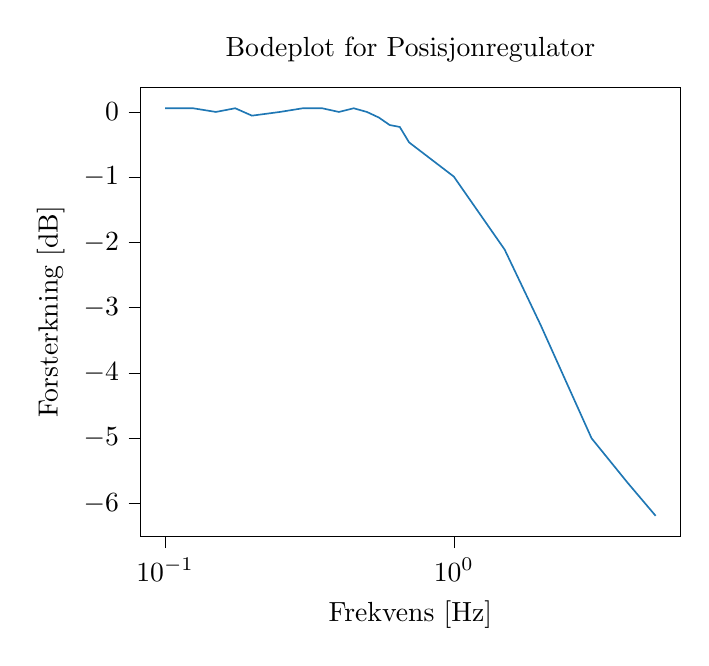
\begin{tikzpicture}

\definecolor{darkgray176}{RGB}{176,176,176}
\definecolor{steelblue31119180}{RGB}{31,119,180}

\begin{axis}[
log basis x={10},
tick align=outside,
tick pos=left,
title={Bodeplot for Posisjonregulator},
x grid style={darkgray176},
xlabel={Frekvens [Hz]},
xmin=0.0822340159426889, xmax=6.08020895329329,
xmode=log,
xtick style={color=black},
xtick={0.001,0.01,0.1,1,10,100},
xticklabels={
  \(\displaystyle {10^{-3}}\),
  \(\displaystyle {10^{-2}}\),
  \(\displaystyle {10^{-1}}\),
  \(\displaystyle {10^{0}}\),
  \(\displaystyle {10^{1}}\),
  \(\displaystyle {10^{2}}\)
},
y grid style={darkgray176},
ylabel={Forsterkning [dB]},
ymin=-6.50506280596274, ymax=0.369045257822048,
ytick style={color=black},
ytick={-7,-6,-5,-4,-3,-2,-1,0,1},
yticklabels={
  \(\displaystyle {\ensuremath{-}7}\),
  \(\displaystyle {\ensuremath{-}6}\),
  \(\displaystyle {\ensuremath{-}5}\),
  \(\displaystyle {\ensuremath{-}4}\),
  \(\displaystyle {\ensuremath{-}3}\),
  \(\displaystyle {\ensuremath{-}2}\),
  \(\displaystyle {\ensuremath{-}1}\),
  \(\displaystyle {0}\),
  \(\displaystyle {1}\)
}
]
\addplot [semithick, steelblue31119180]
table {%
0.1 0.0565858003772851
0.125 0.0565858003772851
0.15 0
0.175 0.0565858003772851
0.2 -0.0569568574565249
0.25 0
0.3 0.0565858003772851
0.35 0.0565858003772851
0.4 0
0.45 0.0565858003772851
0.5 0
0.55 -0.0855759595855004
0.6 -0.201004763143006
0.65 -0.230103248106495
0.7 -0.466468571652479
1 -0.99117558881648
1.5 -2.11020369539948
2 -3.27004263495321
3 -5.00385959148062
4 -5.68648604322257
5 -6.19260334851798
};
\end{axis}

\end{tikzpicture}

    \caption{Bodeplot av posisjonsregulatoren}
    \label{fig:bodeplot}
\end{figure}

\begin{figure}
    \centering
    % This file was created with tikzplotlib v0.10.1.
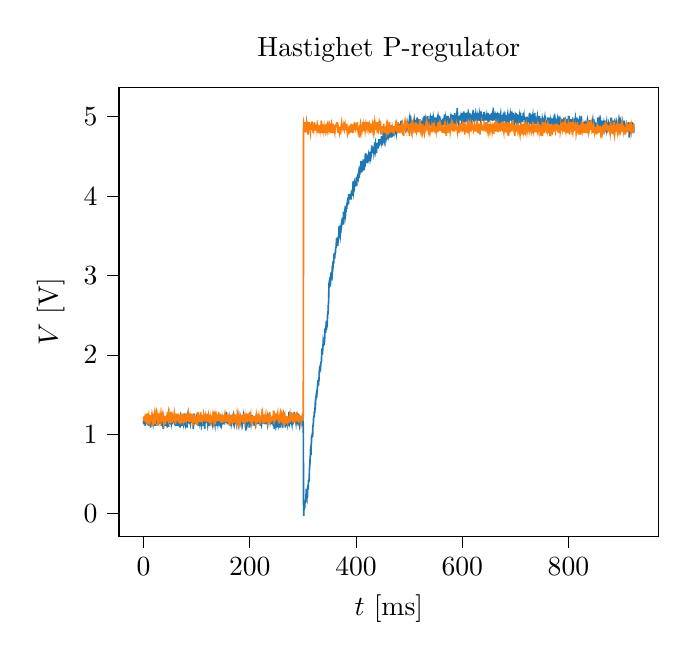
\begin{tikzpicture}

\definecolor{darkgray176}{RGB}{176,176,176}
\definecolor{darkorange25512714}{RGB}{255,127,14}
\definecolor{steelblue31119180}{RGB}{31,119,180}

\begin{axis}[
tick align=outside,
tick pos=left,
title={Hastighet P-regulator},
x grid style={darkgray176},
xlabel={\(\displaystyle t\) [ms]},
xmin=-46.1769, xmax=969.714900000001,
xtick style={color=black},
xtick={-200,0,200,400,600,800,1000},
xticklabels={
  \(\displaystyle {\ensuremath{-}200}\),
  \(\displaystyle {0}\),
  \(\displaystyle {200}\),
  \(\displaystyle {400}\),
  \(\displaystyle {600}\),
  \(\displaystyle {800}\),
  \(\displaystyle {1000}\)
},
y grid style={darkgray176},
ylabel={\(\displaystyle V\) [V]},
ymin=-0.286132745, ymax=5.364255845,
ytick style={color=black},
ytick={-1,0,1,2,3,4,5,6},
yticklabels={
  \(\displaystyle {\ensuremath{-}1}\),
  \(\displaystyle {0}\),
  \(\displaystyle {1}\),
  \(\displaystyle {2}\),
  \(\displaystyle {3}\),
  \(\displaystyle {4}\),
  \(\displaystyle {5}\),
  \(\displaystyle {6}\)
}
]
\addplot [semithick, steelblue31119180]
table {%
0 1.14258
0.462000000000629 1.18164
0.924000000000369 1.12305
1.38600000000011 1.18164
1.84800000000074 1.18164
2.31000000000048 1.2207
2.77200000000022 1.16211
3.23400000000085 1.10352
3.69600000000059 1.2207
4.15800000000033 1.16211
4.62000000000007 1.20117
5.0820000000007 1.14258
5.54400000000044 1.14258
6.00600000000018 1.14258
6.46800000000081 1.14258
6.93000000000055 1.14258
7.39200000000029 1.14258
7.85400000000003 1.20117
8.31600000000066 1.12305
8.7780000000004 1.12305
9.24000000000014 1.20117
9.70200000000077 1.10352
10.1640000000005 1.2207
10.6260000000002 1.12305
11.0880000000009 1.14258
11.5500000000006 1.16211
12.0120000000004 1.2207
12.4740000000001 1.12305
12.9360000000007 1.20117
13.3980000000005 1.08398
13.8600000000002 1.20117
14.3220000000008 1.20117
14.7840000000006 1.12305
15.2460000000003 1.18164
15.7080000000001 1.16211
16.1700000000007 1.16211
16.6320000000004 1.16211
17.0940000000002 1.18164
17.5560000000008 1.14258
18.0180000000005 1.12305
18.4800000000003 1.14258
18.942 1.18164
19.4040000000006 1.2207
19.8660000000004 1.10352
20.3280000000001 1.20117
20.7900000000008 1.14258
21.2520000000005 1.14258
21.7140000000002 1.2207
22.1760000000009 1.2207
22.6380000000006 1.14258
23.1000000000003 1.10352
23.5620000000001 1.20117
24.0240000000007 1.20117
24.4860000000005 1.18164
24.9480000000002 1.18164
25.4100000000008 1.14258
25.8720000000006 1.14258
26.3340000000003 1.25977
26.796 1.2207
27.2580000000007 1.14258
27.7200000000004 1.25977
28.1820000000002 1.16211
28.6440000000008 1.12305
29.1060000000005 1.18164
29.5680000000003 1.14258
30.03 1.2207
30.4920000000006 1.16211
30.9540000000004 1.20117
31.4160000000001 1.14258
31.8780000000007 1.18164
32.3400000000005 1.14258
32.8020000000002 1.14258
33.2640000000008 1.20117
33.7260000000006 1.10352
34.1880000000003 1.16211
34.6500000000001 1.20117
35.1120000000007 1.10352
35.5740000000004 1.14258
36.0360000000002 1.14258
36.4980000000008 1.14258
36.9600000000005 1.06445
37.4220000000003 1.12305
37.884 1.20117
38.3460000000007 1.14258
38.8080000000004 1.20117
39.2700000000001 1.12305
39.7320000000008 1.16211
40.1940000000005 1.10352
40.6560000000002 1.16211
41.1180000000009 1.20117
41.5800000000006 1.2207
42.0420000000004 1.14258
42.5040000000001 1.18164
42.9660000000007 1.2207
43.4280000000005 1.10352
43.8900000000002 1.2207
44.3520000000008 1.20117
44.8140000000006 1.08398
45.2760000000003 1.14258
45.7380000000001 1.18164
46.2000000000007 1.16211
46.6620000000004 1.10352
47.1240000000002 1.10352
47.5860000000008 1.14258
48.0480000000005 1.2207
48.5100000000003 1.14258
48.972 1.14258
49.4340000000006 1.14258
49.8960000000004 1.20117
50.3580000000001 1.2207
50.8200000000008 1.20117
51.2820000000005 1.16211
51.7440000000002 1.14258
52.2060000000009 1.18164
52.6680000000006 1.18164
53.1300000000003 1.16211
53.5920000000001 1.18164
54.0540000000007 1.12305
54.5160000000005 1.20117
54.9780000000002 1.16211
55.4400000000008 1.20117
55.9020000000006 1.14258
56.3640000000003 1.18164
56.826 1.18164
57.2880000000007 1.18164
57.7500000000004 1.18164
58.2120000000002 1.16211
58.6740000000008 1.18164
59.1360000000005 1.12305
59.5980000000003 1.16211
60.06 1.14258
60.5220000000006 1.14258
60.9840000000004 1.10352
61.4460000000001 1.16211
61.9080000000007 1.20117
62.3700000000005 1.10352
62.8320000000002 1.14258
63.2940000000008 1.14258
63.7560000000006 1.20117
64.2180000000003 1.14258
64.6800000000001 1.14258
65.1420000000007 1.12305
65.6040000000004 1.10352
66.0660000000002 1.2207
66.5280000000008 1.14258
66.9900000000005 1.20117
67.4520000000003 1.14258
67.914 1.2207
68.3760000000007 1.08398
68.8380000000004 1.14258
69.3000000000001 1.18164
69.7620000000008 1.16211
70.2240000000005 1.20117
70.6860000000002 1.18164
71.1480000000009 1.16211
71.6100000000006 1.10352
72.0720000000004 1.20117
72.5340000000001 1.10352
72.9960000000007 1.2207
73.4580000000005 1.2207
73.9200000000002 1.14258
74.3820000000008 1.16211
74.8440000000006 1.14258
75.3060000000003 1.18164
75.7680000000001 1.25977
76.2300000000007 1.18164
76.6920000000004 1.16211
77.1540000000002 1.18164
77.6160000000008 1.14258
78.0780000000005 1.2207
78.5400000000003 1.14258
79.002 1.12305
79.4640000000007 1.14258
79.9260000000004 1.20117
80.3880000000001 1.2207
80.8500000000008 1.10352
81.3120000000005 1.16211
81.7740000000002 1.08398
82.2360000000009 1.14258
82.6980000000006 1.18164
83.1600000000003 1.2207
83.6220000000001 1.20117
84.0840000000007 1.2207
84.5460000000004 1.20117
85.0080000000002 1.20117
85.4700000000008 1.14258
85.9320000000006 1.20117
86.3940000000003 1.12305
86.8560000000001 1.14258
87.3180000000007 1.18164
87.7800000000004 1.16211
88.2420000000002 1.14258
88.7040000000008 1.18164
89.1660000000005 1.20117
89.6280000000003 1.20117
90.09 1.14258
90.5520000000006 1.18164
91.0140000000004 1.18164
91.4760000000001 1.18164
91.9380000000007 1.20117
92.4000000000005 1.24023
92.8620000000002 1.20117
93.3240000000009 1.14258
93.7860000000006 1.06445
94.2480000000003 1.16211
94.7100000000001 1.20117
95.1720000000007 1.12305
95.6340000000004 1.25977
96.0960000000002 1.2207
96.5580000000008 1.14258
97.0200000000006 1.14258
97.4820000000003 1.14258
97.944 1.16211
98.4060000000007 1.20117
98.8680000000004 1.20117
99.3300000000001 1.18164
99.7920000000008 1.20117
100.254000000001 1.18164
100.716 1.18164
101.178000000001 1.14258
101.640000000001 1.14258
102.102 1.14258
102.564 1.18164
103.026000000001 1.10352
103.488 1.14258
103.95 1.14258
104.412000000001 1.14258
104.874000000001 1.14258
105.336 1.16211
105.798 1.14258
106.260000000001 1.18164
106.722 1.14258
107.184 1.18164
107.646000000001 1.10352
108.108000000001 1.16211
108.57 1.10352
109.032 1.16211
109.494000000001 1.12305
109.956 1.14258
110.418 1.16211
110.880000000001 1.16211
111.342 1.10352
111.804 1.2207
112.266000000001 1.12305
112.728000000001 1.14258
113.19 1.16211
113.652 1.14258
114.114000000001 1.12305
114.576 1.20117
115.038 1.06445
115.500000000001 1.14258
115.962000000001 1.14258
116.424 1.20117
116.886 1.20117
117.348000000001 1.14258
117.81 1.20117
118.272 1.18164
118.734000000001 1.18164
119.196000000001 1.2207
119.658 1.18164
120.12 1.16211
120.582000000001 1.16211
121.044 1.12305
121.506 1.14258
121.968000000001 1.18164
122.43 1.18164
122.892 1.2207
123.354000000001 1.14258
123.816000000001 1.20117
124.278 1.10352
124.74 1.20117
125.202000000001 1.14258
125.664 1.18164
126.126 1.12305
126.588000000001 1.20117
127.050000000001 1.14258
127.512 1.2207
127.974 1.18164
128.436000000001 1.2207
128.898 1.16211
129.36 1.14258
129.822000000001 1.18164
130.284000000001 1.18164
130.746 1.10352
131.208000000001 1.14258
131.670000000001 1.14258
132.132 1.18164
132.594 1.16211
133.056000000001 1.2793
133.518 1.12305
133.98 1.14258
134.442000000001 1.12305
134.904000000001 1.18164
135.366 1.14258
135.828 1.2207
136.290000000001 1.14258
136.752 1.18164
137.214 1.10352
137.676000000001 1.14258
138.138000000001 1.14258
138.6 1.10352
139.062 1.16211
139.524000000001 1.14258
139.986 1.20117
140.448 1.20117
140.910000000001 1.12305
141.372 1.20117
141.834 1.14258
142.296000000001 1.14258
142.758000000001 1.18164
143.22 1.10352
143.682 1.16211
144.144000000001 1.14258
144.606 1.16211
145.068 1.16211
145.530000000001 1.08398
145.992000000001 1.20117
146.454 1.14258
146.916 1.18164
147.378000000001 1.14258
147.84 1.16211
148.302 1.20117
148.764000000001 1.18164
149.226000000001 1.20117
149.688 1.20117
150.15 1.2207
150.612000000001 1.14258
151.074 1.2207
151.536 1.12305
151.998000000001 1.14258
152.46 1.16211
152.922 1.20117
153.384000000001 1.14258
153.846000000001 1.18164
154.308 1.18164
154.77 1.14258
155.232000000001 1.18164
155.694 1.14258
156.156 1.2793
156.618000000001 1.2207
157.080000000001 1.14258
157.542 1.16211
158.004 1.12305
158.466000000001 1.18164
158.928 1.24023
159.39 1.16211
159.852000000001 1.18164
160.314000000001 1.20117
160.776 1.20117
161.238000000001 1.2207
161.700000000001 1.20117
162.162 1.10352
162.624 1.14258
163.086000000001 1.16211
163.548 1.16211
164.01 1.14258
164.472000000001 1.14258
164.934000000001 1.18164
165.396 1.14258
165.858 1.16211
166.320000000001 1.14258
166.782 1.2207
167.244 1.14258
167.706000000001 1.18164
168.168000000001 1.18164
168.63 1.20117
169.092 1.16211
169.554000000001 1.18164
170.016 1.14258
170.478 1.20117
170.940000000001 1.18164
171.402 1.14258
171.864 1.16211
172.326000000001 1.20117
172.788000000001 1.16211
173.25 1.20117
173.712 1.2207
174.174000000001 1.14258
174.636 1.18164
175.098 1.14258
175.560000000001 1.16211
176.022000000001 1.16211
176.484 1.14258
176.946 1.12305
177.408000000001 1.20117
177.87 1.18164
178.332 1.14258
178.794000000001 1.16211
179.256000000001 1.14258
179.718 1.20117
180.18 1.14258
180.642000000001 1.20117
181.104 1.14258
181.566 1.14258
182.028000000001 1.20117
182.49 1.18164
182.952 1.16211
183.414000000001 1.14258
183.876000000001 1.20117
184.338 1.16211
184.8 1.16211
185.262000000001 1.18164
185.724 1.16211
186.186 1.14258
186.648000000001 1.18164
187.110000000001 1.20117
187.572 1.16211
188.034 1.14258
188.496000000001 1.14258
188.958 1.16211
189.42 1.2207
189.882000000001 1.20117
190.344000000001 1.16211
190.806 1.16211
191.268 1.14258
191.730000000001 1.20117
192.192 1.14258
192.654 1.04492
193.116000000001 1.18164
193.578 1.16211
194.04 1.12305
194.502000000001 1.14258
194.964000000001 1.12305
195.426 1.14258
195.888 1.2207
196.350000000001 1.12305
196.812 1.2207
197.274 1.2207
197.736000000001 1.2207
198.198000000001 1.14258
198.66 1.2207
199.122 1.08398
199.584000000001 1.14258
200.046 1.2207
200.508 1.16211
200.970000000001 1.20117
201.432 1.12305
201.894 1.14258
202.356000000001 1.18164
202.818000000001 1.14258
203.28 1.16211
203.742 1.16211
204.204000000001 1.24023
204.666 1.14258
205.128 1.20117
205.590000000001 1.20117
206.052000000001 1.14258
206.514 1.2207
206.976 1.2207
207.438000000001 1.12305
207.9 1.18164
208.362 1.10352
208.824000000001 1.18164
209.286000000001 1.14258
209.748 1.14258
210.21 1.20117
210.672000000001 1.16211
211.134 1.18164
211.596 1.14258
212.058000000001 1.16211
212.52 1.14258
212.982 1.14258
213.444000000001 1.20117
213.906000000001 1.20117
214.368 1.14258
214.83 1.14258
215.292000000001 1.14258
215.754 1.18164
216.216 1.12305
216.678000000001 1.16211
217.140000000001 1.16211
217.602 1.14258
218.064 1.14258
218.526000000001 1.2207
218.988 1.20117
219.45 1.14258
219.912000000001 1.18164
220.374000000001 1.10352
220.836 1.18164
221.298 1.18164
221.760000000001 1.14258
222.222 1.12305
222.684 1.14258
223.146000000001 1.18164
223.608 1.18164
224.07 1.18164
224.532000000001 1.2207
224.994000000001 1.16211
225.456 1.14258
225.918 1.14258
226.380000000001 1.14258
226.842 1.18164
227.304 1.14258
227.766000000001 1.20117
228.228000000001 1.20117
228.69 1.16211
229.152 1.12305
229.614000000001 1.20117
230.076 1.16211
230.538 1.20117
231.000000000001 1.14258
231.462000000001 1.14258
231.924 1.16211
232.386000000001 1.2207
232.848000000001 1.18164
233.31 1.20117
233.772 1.14258
234.234000000001 1.16211
234.696 1.14258
235.158 1.2207
235.620000000001 1.20117
236.082000000001 1.14258
236.544 1.18164
237.006 1.20117
237.468000000001 1.20117
237.93 1.18164
238.392 1.2207
238.854000000001 1.14258
239.316000000001 1.14258
239.778 1.18164
240.24 1.20117
240.702000000001 1.12305
241.164 1.20117
241.626 1.12305
242.088000000001 1.20117
242.55 1.18164
243.012 1.14258
243.474000000001 1.20117
243.936000000001 1.20117
244.398 1.10352
244.86 1.16211
245.322000000001 1.18164
245.784 1.14258
246.246 1.06445
246.708000000001 1.14258
247.170000000001 1.14258
247.632 1.12305
248.094 1.16211
248.556000000001 1.14258
249.018 1.08398
249.48 1.16211
249.942000000001 1.14258
250.404000000001 1.18164
250.866 1.2207
251.328 1.10352
251.790000000001 1.10352
252.252 1.10352
252.714 1.12305
253.176000000001 1.16211
253.638 1.08398
254.1 1.12305
254.562000000001 1.20117
255.024000000001 1.14258
255.486 1.16211
255.948 1.20117
256.410000000001 1.2207
256.872 1.08398
257.334 1.10352
257.796000000001 1.14258
258.258000000001 1.20117
258.72 1.24023
259.182 1.20117
259.644000000001 1.18164
260.106 1.18164
260.568 1.18164
261.030000000001 1.14258
261.492000000001 1.16211
261.954 1.08398
262.416000000001 1.16211
262.878000000001 1.16211
263.34 1.2207
263.802 1.20117
264.264000000001 1.14258
264.726 1.20117
265.188 1.18164
265.650000000001 1.14258
266.112000000001 1.14258
266.574 1.14258
267.036 1.08398
267.498000000001 1.12305
267.96 1.20117
268.422 1.20117
268.884000000001 1.16211
269.346000000001 1.16211
269.808 1.10352
270.27 1.18164
270.732000000001 1.14258
271.194 1.20117
271.656 1.14258
272.118000000001 1.16211
272.58 1.18164
273.042 1.20117
273.504000000001 1.10352
273.966000000001 1.2793
274.428 1.16211
274.89 1.14258
275.352000000001 1.16211
275.814 1.12305
276.276 1.18164
276.738000000001 1.18164
277.200000000001 1.25977
277.662 1.20117
278.124 1.14258
278.586000000001 1.24023
279.048 1.14258
279.51 1.12305
279.972000000001 1.16211
280.434000000001 1.14258
280.896 1.24023
281.358 1.12305
281.820000000001 1.18164
282.282 1.14258
282.744 1.20117
283.206000000001 1.2207
283.668 1.2793
284.13 1.14258
284.592000000001 1.2207
285.054000000001 1.18164
285.516 1.2207
285.978 1.16211
286.440000000001 1.16211
286.902 1.14258
287.364 1.18164
287.826000000001 1.14258
288.288000000001 1.14258
288.75 1.16211
289.212 1.20117
289.674000000001 1.12305
290.136 1.18164
290.598 1.16211
291.060000000001 1.18164
291.522000000001 1.25977
291.984 1.20117
292.446000000001 1.16211
292.908000000001 1.14258
293.37 1.12305
293.832 1.16211
294.294000000001 1.14258
294.756 1.18164
295.218 1.14258
295.680000000001 1.2207
296.142000000001 1.16211
296.604 1.20117
297.066 1.2207
297.528000000001 1.14258
297.99 1.16211
298.452 1.12305
298.914000000001 1.12305
299.376000000001 1.14258
299.838 1.2207
300.3 1.10352
300.762000000001 1.14258
301.224 0.126953
301.686 -0.0292969
302.148000000001 0.107422
302.61 0.126953
303.072 0.126953
303.534000000001 0.0683594
303.996000000001 0.166016
304.458 0.146484
304.92 0.146484
305.382000000001 0.166016
305.844 0.224609
306.306 0.205078
306.768000000001 0.166016
307.230000000001 0.224609
307.692 0.205078
308.154 0.263672
308.616000000001 0.205078
309.078 0.322266
309.54 0.361328
310.002000000001 0.302734
310.464000000001 0.419922
310.926 0.400391
311.388 0.419922
311.850000000001 0.419922
312.312 0.556641
312.774 0.595703
313.236000000001 0.634766
313.698 0.712891
314.16 0.732422
314.622000000001 0.849609
315.084000000001 0.732422
315.546 0.849609
316.008 0.888672
316.470000000001 0.986328
316.932 0.966797
317.394 0.986328
317.856000000001 1.00586
318.318000000001 0.966797
318.78 1.10352
319.242 1.10352
319.704000000001 1.14258
320.166 1.20117
320.628 1.2207
321.090000000001 1.2207
321.552 1.2793
322.014 1.2793
322.476000000001 1.2793
322.938000000001 1.33789
323.4 1.31836
323.862 1.43555
324.324000000001 1.43555
324.786 1.47461
325.248 1.49414
325.710000000001 1.45508
326.172000000001 1.49414
326.634 1.51367
327.096 1.55273
327.558000000001 1.61133
328.02 1.63086
328.482 1.66992
328.944000000001 1.66992
329.406000000001 1.61133
329.868 1.68945
330.33 1.68945
330.792000000001 1.78711
331.254 1.80664
331.716 1.8457
332.178000000001 1.8457
332.64 1.78711
333.102 1.88477
333.564000000001 1.86523
334.026000000001 1.9043
334.488 1.9043
334.95 1.92383
335.412000000001 2.04102
335.874 2.08008
336.336 2.00195
336.798000000001 2.02148
337.260000000001 2.06055
337.722 2.09961
338.184 2.1582
338.646000000001 2.13867
339.108 2.2168
339.57 2.11914
340.032000000001 2.2168
340.494000000001 2.1582
340.956 2.19727
341.418 2.29492
341.880000000001 2.33398
342.342 2.29492
342.804 2.27539
343.266000000001 2.37305
343.728 2.35352
344.19 2.43164
344.652000000001 2.31445
345.114000000001 2.43164
345.576 2.35352
346.038 2.43164
346.500000000001 2.50977
346.962 2.5293
347.424 2.50977
347.886000000001 2.62695
348.348000000001 2.66602
348.81 2.80273
349.272 2.90039
349.734000000001 2.91992
350.196 2.90039
350.658 2.91992
351.120000000001 2.91992
351.582000000001 2.86133
352.044 2.91992
352.506000000001 2.97852
352.968000000001 3.03711
353.43 2.93945
353.892 3.01758
354.354000000001 2.97852
354.816 3.03711
355.278 3.01758
355.740000000001 3.05664
356.202000000001 3.0957
356.664 3.17383
357.126 3.1543
357.588000000001 3.19336
358.05 3.1543
358.512 3.25195
358.974000000001 3.27148
359.436000000001 3.27148
359.898 3.21289
360.36 3.27148
360.822000000001 3.29102
361.284 3.29102
361.746 3.34961
362.208000000001 3.34961
362.67 3.36914
363.132 3.44727
363.594000000001 3.4668
364.056000000001 3.4668
364.518 3.36914
364.98 3.4082
365.442000000001 3.36914
365.904 3.4082
366.366 3.42773
366.828000000001 3.4668
367.290000000001 3.50586
367.752 3.54492
368.214 3.62305
368.676000000001 3.56445
369.138 3.56445
369.6 3.52539
370.062000000001 3.50586
370.524000000001 3.56445
370.986 3.54492
371.448 3.54492
371.910000000001 3.62305
372.372 3.62305
372.834 3.60352
373.296000000001 3.70117
373.758 3.66211
374.22 3.7207
374.682000000001 3.66211
375.144000000001 3.7207
375.606 3.7207
376.068 3.64258
376.530000000001 3.79883
376.992 3.7207
377.454 3.7207
377.916000000001 3.79883
378.378000000001 3.79883
378.84 3.81836
379.302 3.79883
379.764000000001 3.74023
380.226 3.75977
380.688 3.87695
381.150000000001 3.79883
381.612000000001 3.87695
382.074 3.85742
382.536000000001 3.83789
382.998000000001 3.91602
383.46 3.87695
383.922 3.93555
384.384000000001 3.93555
384.846 3.97461
385.308 3.97461
385.770000000001 3.89648
386.232000000001 4.01367
386.694 4.01367
387.156 3.99414
387.618000000001 3.95508
388.08 4.01367
388.542 3.97461
389.004000000001 3.97461
389.466000000001 4.01367
389.928 4.0332
390.39 3.95508
390.852000000001 4.01367
391.314 4.01367
391.776 4.07227
392.238000000001 4.01367
392.700000000001 4.01367
393.162 4.05273
393.624000000001 4.0918
394.086000000001 4.05273
394.548 4.18945
395.01 4.11133
395.472000000001 4.05273
395.934 4.07227
396.396 4.15039
396.858000000001 4.16992
397.320000000001 4.15039
397.782 4.18945
398.244 4.15039
398.706000000001 4.13086
399.168 4.13086
399.63 4.18945
400.092000000001 4.15039
400.554000000001 4.22852
401.016 4.13086
401.478 4.15039
401.940000000001 4.22852
402.402 4.22852
402.864 4.24805
403.326000000001 4.26758
403.788 4.26758
404.25 4.24805
404.712000000001 4.28711
405.174000000001 4.30664
405.636 4.26758
406.098 4.22852
406.560000000001 4.32617
407.022 4.26758
407.484 4.32617
407.946000000001 4.36523
408.408000000001 4.36523
408.87 4.32617
409.332 4.44336
409.794000000001 4.4043
410.256 4.30664
410.718 4.30664
411.180000000001 4.32617
411.642000000001 4.32617
412.104 4.32617
412.566000000001 4.36523
413.028000000001 4.4043
413.49 4.46289
413.952 4.38477
414.414000000001 4.44336
414.876 4.3457
415.338 4.32617
415.800000000001 4.4043
416.262000000001 4.38477
416.724 4.36523
417.186 4.50195
417.648000000001 4.50195
418.11 4.54102
418.572 4.50195
419.034000000001 4.48242
419.496000000001 4.50195
419.958 4.52148
420.42 4.42383
420.882000000001 4.44336
421.344 4.42383
421.806 4.42383
422.268000000001 4.46289
422.73 4.46289
423.192 4.50195
423.654000000001 4.52148
424.116000000001 4.50195
424.578 4.56055
425.04 4.44336
425.502000000001 4.48242
425.964 4.48242
426.426 4.54102
426.888000000001 4.50195
427.350000000001 4.46289
427.812 4.56055
428.274 4.50195
428.736000000001 4.52148
429.198 4.58008
429.66 4.63867
430.122000000001 4.54102
430.584000000001 4.61914
431.046 4.58008
431.508 4.58008
431.970000000001 4.58008
432.432 4.56055
432.894 4.56055
433.356000000001 4.58008
433.818 4.54102
434.28 4.56055
434.742000000001 4.58008
435.204000000001 4.67773
435.666 4.59961
436.128 4.58008
436.590000000001 4.61914
437.052 4.6582
437.514 4.63867
437.976000000001 4.58008
438.438000000001 4.54102
438.9 4.63867
439.362 4.6582
439.824000000001 4.6582
440.286 4.61914
440.748 4.6582
441.210000000001 4.59961
441.672 4.67773
442.134 4.6582
442.596000000001 4.61914
443.058000000001 4.7168
443.52 4.6582
443.982 4.7168
444.444000000001 4.63867
444.906 4.6582
445.368 4.67773
445.830000000001 4.69727
446.292000000001 4.69727
446.754 4.69727
447.216 4.7168
447.678000000001 4.7168
448.14 4.75586
448.602 4.69727
449.064000000001 4.7168
449.526000000001 4.7168
449.988 4.69727
450.45 4.7168
450.912000000001 4.7168
451.374 4.81445
451.836 4.73633
452.298000000001 4.7168
452.760000000001 4.75586
453.222 4.77539
453.684000000001 4.7168
454.146000000001 4.73633
454.608 4.7168
455.07 4.77539
455.532000000001 4.87305
455.994 4.79492
456.456 4.75586
456.918000000001 4.79492
457.380000000001 4.75586
457.842 4.77539
458.304 4.7168
458.766000000001 4.77539
459.228 4.79492
459.69 4.73633
460.152000000001 4.73633
460.614000000001 4.83398
461.076 4.77539
461.538 4.75586
462.000000000001 4.77539
462.462 4.79492
462.924 4.73633
463.386000000001 4.79492
463.848 4.79492
464.31 4.79492
464.772000000001 4.85352
465.234000000001 4.81445
465.696 4.79492
466.158 4.79492
466.620000000001 4.73633
467.082 4.79492
467.544 4.75586
468.006000000001 4.75586
468.468000000001 4.83398
468.93 4.79492
469.392 4.87305
469.854000000001 4.85352
470.316 4.79492
470.778 4.85352
471.240000000001 4.75586
471.702000000001 4.81445
472.164 4.85352
472.626000000001 4.81445
473.088000000001 4.77539
473.55 4.85352
474.012 4.83398
474.474000000001 4.85352
474.936 4.87305
475.398 4.81445
475.860000000001 4.85352
476.322000000001 4.79492
476.784 4.81445
477.246 4.85352
477.708000000001 4.81445
478.17 4.81445
478.632 4.87305
479.094000000001 4.91211
479.556000000001 4.87305
480.018 4.83398
480.48 4.89258
480.942000000001 4.81445
481.404 4.91211
481.866 4.83398
482.328000000001 4.81445
482.79 4.81445
483.252 4.85352
483.714000000001 4.79492
484.176000000001 4.85352
484.638 4.93164
485.1 4.95117
485.562000000001 4.87305
486.024 4.91211
486.486 4.87305
486.948000000001 4.87305
487.410000000001 4.85352
487.872 4.89258
488.334 4.83398
488.796000000001 4.87305
489.258 4.83398
489.72 4.83398
490.182000000001 4.87305
490.644000000001 4.83398
491.106 4.89258
491.568 4.89258
492.030000000001 4.93164
492.492 4.89258
492.954 4.87305
493.416000000001 4.91211
493.878 4.93164
494.34 4.93164
494.802000000001 4.81445
495.264000000001 4.93164
495.726 4.87305
496.188 4.87305
496.650000000001 4.91211
497.112 4.89258
497.574 4.87305
498.036000000001 4.91211
498.498000000001 4.87305
498.96 4.89258
499.422 4.91211
499.884000000001 4.89258
500.346 4.93164
500.808 4.91211
501.270000000001 4.91211
501.732000000001 4.9707
502.194 4.95117
502.656000000001 5.00977
503.118000000001 4.93164
503.58 4.93164
504.042 4.93164
504.504000000001 4.87305
504.966 4.89258
505.428 4.87305
505.890000000001 4.87305
506.352000000001 4.89258
506.814 4.87305
507.276 4.91211
507.738000000001 4.83398
508.2 4.95117
508.662 4.93164
509.124000000001 4.95117
509.586000000001 4.89258
510.048 4.93164
510.51 4.87305
510.972000000001 4.91211
511.434 4.89258
511.896 4.95117
512.358000000001 4.95117
512.820000000001 4.87305
513.282 4.91211
513.744000000001 4.91211
514.206000000001 4.95117
514.668 4.95117
515.13 4.99023
515.592000000001 4.95117
516.054 4.81445
516.516 4.9707
516.978000000001 4.91211
517.440000000001 4.91211
517.902 4.93164
518.364 4.95117
518.826000000001 4.81445
519.288 4.95117
519.75 4.9707
520.212000000001 4.87305
520.674000000001 4.95117
521.136 4.95117
521.598 4.93164
522.060000000001 4.91211
522.522 4.95117
522.984 4.89258
523.446000000001 4.91211
523.908 4.91211
524.37 4.89258
524.832000000001 4.91211
525.294000000001 4.91211
525.756 4.95117
526.218 4.91211
526.680000000001 4.99023
527.142 4.83398
527.604 4.99023
528.066000000001 4.91211
528.528000000001 5.00977
528.99 4.93164
529.452 4.91211
529.914000000001 4.9707
530.376 4.89258
530.838 4.95117
531.300000000001 4.93164
531.762000000001 4.99023
532.224 4.95117
532.686 4.93164
533.148000000001 4.95117
533.61 4.93164
534.072 4.89258
534.534000000001 4.91211
534.996 5.00977
535.458 4.89258
535.920000000001 4.9707
536.382000000001 4.93164
536.844 4.9707
537.306 4.93164
537.768000000001 4.93164
538.23 4.85352
538.692 4.95117
539.154000000001 4.89258
539.616000000001 5.00977
540.078 4.93164
540.54 4.9707
541.002000000001 4.95117
541.464 4.99023
541.926 4.91211
542.388000000001 4.95117
542.85 4.89258
543.312 5.00977
543.774000000001 4.91211
544.236000000001 4.99023
544.698 4.9707
545.16 4.95117
545.622000000001 4.99023
546.084000000001 4.9707
546.546 4.95117
547.008000000001 4.9707
547.470000000001 4.99023
547.932 4.91211
548.394 4.87305
548.856000000001 4.95117
549.318 4.87305
549.78 4.95117
550.242000000001 4.99023
550.704000000001 4.93164
551.166 4.95117
551.628 4.99023
552.090000000001 4.93164
552.552 4.95117
553.014 4.93164
553.476000000001 4.91211
553.938 4.99023
554.4 5.00977
554.862000000001 4.99023
555.324000000001 4.95117
555.786 4.87305
556.248 4.95117
556.710000000001 4.93164
557.172 5.00977
557.634 4.89258
558.096000000001 4.93164
558.558000000001 4.91211
559.02 4.89258
559.482 4.91211
559.944000000001 4.87305
560.406 4.95117
560.868 4.95117
561.330000000001 4.87305
561.792 4.95117
562.254 4.91211
562.716 4.91211
563.178000000001 4.93164
563.64 4.9707
564.102 4.93164
564.564000000001 4.99023
565.026000000001 4.93164
565.488 4.99023
565.950000000001 4.89258
566.412000000001 5.0293
566.874 4.93164
567.336 4.93164
567.798000000001 4.87305
568.26 4.95117
568.722 4.91211
569.184000000001 4.9707
569.646000000001 4.95117
570.108 5.00977
570.57 4.91211
571.032000000001 5.00977
571.494 4.95117
571.956 4.93164
572.418000000001 4.99023
572.88 4.89258
573.342 4.95117
573.804000000001 5.00977
574.266000000001 4.93164
574.728 4.93164
575.19 4.95117
575.652000000001 4.9707
576.114 4.9707
576.576 4.9707
577.038000000001 4.93164
577.500000000001 4.95117
577.962 4.9707
578.424 4.93164
578.886000000001 5.0293
579.348 4.9707
579.81 4.95117
580.272000000001 4.95117
580.734 4.89258
581.196 4.95117
581.658 4.93164
582.120000000001 4.91211
582.582 5.00977
583.044 5.00977
583.506000000001 4.89258
583.968000000001 5.00977
584.43 4.9707
584.892000000001 4.95117
585.354000000001 4.91211
585.816 5.04883
586.278 4.93164
586.740000000001 4.95117
587.202 4.87305
587.664 4.95117
588.126000000001 4.93164
588.588000000001 4.91211
589.05 4.93164
589.512 5.00977
589.974000000001 5.00977
590.436 5.10742
590.898 5.04883
591.360000000001 5.00977
591.822000000001 4.9707
592.284 4.95117
592.746 4.93164
593.208000000001 4.87305
593.67 4.95117
594.132 5.00977
594.594000000001 4.9707
595.056 4.9707
595.518 4.9707
595.980000000001 4.9707
596.442000000001 4.99023
596.904 5.0293
597.366 4.95117
597.828000000001 4.99023
598.29 4.9707
598.752 5.00977
599.214000000001 4.9707
599.676 4.95117
600.138 4.91211
600.6 5.04883
601.062000000001 4.99023
601.524 5.00977
601.986 5.00977
602.448000000001 4.95117
602.910000000001 5.06836
603.372 4.9707
603.834000000001 4.93164
604.296000000001 5.00977
604.758 4.99023
605.22 5.04883
605.682000000001 4.93164
606.144 5.04883
606.606 5.0293
607.068000000001 4.95117
607.530000000001 4.95117
607.992 4.9707
608.454 4.99023
608.916000000001 5.00977
609.378 4.9707
609.84 5.04883
610.302000000001 4.99023
610.764000000001 5.00977
611.226 5.04883
611.688 4.95117
612.150000000001 5.00977
612.612 4.99023
613.074 4.9707
613.536000000001 4.99023
613.998000000001 5.04883
614.46 5.00977
614.922000000001 4.95117
615.384000000001 4.99023
615.846 5.00977
616.308 5.00977
616.770000000001 4.99023
617.232 5.0293
617.694 4.99023
618.156000000001 5.0293
618.618000000001 4.99023
619.08 5.00977
619.542 4.9707
620.004000000001 4.9707
620.466 5.08789
620.928 4.9707
621.390000000001 5.00977
621.852000000001 5.00977
622.314 4.93164
622.776 4.99023
623.238000000001 5.04883
623.7 4.9707
624.162 4.99023
624.624000000001 5.00977
625.086 4.95117
625.548 5.00977
626.010000000001 4.99023
626.472000000001 5.0293
626.934 4.9707
627.396 5.00977
627.858000000001 4.9707
628.32 5.00977
628.782 4.99023
629.244000000001 5.00977
629.706000000001 5.00977
630.168 5.0293
630.63 5.04883
631.092000000001 4.95117
631.554 4.9707
632.016 4.9707
632.478000000001 5.0293
632.940000000001 5.00977
633.402 4.99023
633.864000000001 5.00977
634.326000000001 4.99023
634.788 4.95117
635.25 4.9707
635.712000000001 5.06836
636.174 4.95117
636.636 4.9707
637.098000000001 4.99023
637.560000000001 4.99023
638.022 5.0293
638.484 4.9707
638.946000000001 4.95117
639.408 5.0293
639.87 5.00977
640.332000000001 4.99023
640.794000000001 5.04883
641.256 5.04883
641.718 4.95117
642.180000000001 4.99023
642.642 5.00977
643.104 4.99023
643.566000000001 4.99023
644.028 4.95117
644.49 5.00977
644.952000000001 4.95117
645.414000000001 4.99023
645.876 5.00977
646.338 4.9707
646.800000000001 4.9707
647.262 5.0293
647.724 4.99023
648.186000000001 5.00977
648.648000000001 5.04883
649.11 5.00977
649.572 4.9707
650.034000000001 4.93164
650.496 4.99023
650.958 4.99023
651.420000000001 5.0293
651.882000000001 4.95117
652.344 5.00977
652.806 4.9707
653.268000000001 4.9707
653.73 4.99023
654.192 4.99023
654.654000000001 4.99023
655.116 5.04883
655.578 4.99023
656.040000000001 4.95117
656.502000000001 5.00977
656.964 5.0293
657.426 4.9707
657.888000000001 4.95117
658.35 5.0293
658.812 5.0293
659.274000000001 4.9707
659.736000000001 5.0293
660.198 5.00977
660.66 4.95117
661.122000000001 4.99023
661.584 5.0293
662.046 5.04883
662.508000000001 4.95117
662.97 4.99023
663.432 4.9707
663.894000000001 5.0293
664.356000000001 5.0293
664.818 5.0293
665.28 5.04883
665.742000000001 4.9707
666.204 4.95117
666.666 4.99023
667.128000000001 4.9707
667.590000000001 4.95117
668.052 5.04883
668.514 4.9707
668.976000000001 4.95117
669.438 4.9707
669.9 4.95117
670.362000000001 4.9707
670.824000000001 5.00977
671.286 5.00977
671.748 5.00977
672.210000000001 5.0293
672.672 4.9707
673.134 4.99023
673.596000000001 4.9707
674.058 5.00977
674.52 5.00977
674.982000000001 4.99023
675.444000000001 4.99023
675.906 4.9707
676.368 4.99023
676.830000000001 4.9707
677.292 4.99023
677.754 4.9707
678.216000000001 4.95117
678.678000000001 4.95117
679.14 4.99023
679.602 4.9707
680.064000000001 5.04883
680.526 4.95117
680.988 4.99023
681.450000000001 4.9707
681.912 5.00977
682.374 5.00977
682.836 4.99023
683.298000000001 4.9707
683.76 4.95117
684.222 4.9707
684.684000000001 4.9707
685.146000000001 5.00977
685.608 5.0293
686.070000000001 4.99023
686.532000000001 4.99023
686.994 4.95117
687.456 4.9707
687.918000000001 5.0293
688.38 5.0293
688.842 4.9707
689.304000000001 4.99023
689.766000000001 5.00977
690.228 5.0293
690.69 4.99023
691.152000000001 4.9707
691.614 4.9707
692.076 4.9707
692.538000000001 4.95117
693 5.06836
693.462 4.9707
693.924000000001 4.95117
694.386000000001 4.93164
694.848 5.04883
695.31 4.95117
695.772000000001 4.91211
696.234 4.9707
696.696 4.99023
697.158000000001 4.9707
697.620000000001 4.95117
698.082 4.9707
698.544 4.9707
699.006000000001 4.99023
699.468 4.95117
699.93 4.9707
700.392000000001 5.00977
700.854 4.93164
701.316 5.04883
701.778 5.00977
702.240000000001 5.00977
702.702 4.95117
703.164 4.9707
703.626000000001 4.9707
704.088000000001 5.0293
704.55 4.95117
705.012000000001 4.95117
705.474000000001 4.93164
705.936 4.95117
706.398 4.93164
706.860000000001 4.93164
707.322 4.95117
707.784 5.00977
708.246000000001 4.99023
708.708000000001 5.04883
709.17 5.00977
709.632 4.9707
710.094000000001 4.99023
710.556 4.95117
711.018 4.9707
711.480000000001 5.00977
711.942 4.95117
712.404 4.95117
712.866 4.9707
713.328000000001 5.00977
713.79 4.93164
714.252 4.9707
714.714000000001 5.04883
715.176 4.99023
715.638 4.99023
716.100000000001 5.00977
716.562000000001 4.9707
717.024 4.9707
717.486 4.99023
717.948000000001 4.99023
718.41 4.95117
718.872 4.91211
719.334000000001 4.89258
719.796000000001 4.93164
720.258 4.93164
720.72 4.9707
721.182000000001 4.93164
721.644 4.99023
722.106 4.99023
722.568000000001 4.95117
723.030000000001 4.93164
723.492 4.9707
723.954000000001 4.9707
724.416000000001 4.9707
724.878 4.93164
725.34 4.99023
725.802000000001 4.93164
726.264 5.0293
726.726 4.93164
727.188000000001 5.04883
727.650000000001 4.91211
728.112 5.00977
728.574 4.95117
729.036000000001 4.95117
729.498 4.95117
729.96 4.95117
730.422000000001 4.9707
730.884000000001 5.0293
731.346 4.89258
731.808 4.95117
732.270000000001 4.99023
732.732 5.00977
733.194 4.95117
733.656000000001 4.91211
734.118000000001 4.99023
734.58 4.89258
735.042000000001 4.99023
735.504000000001 4.93164
735.966 4.91211
736.428 5.04883
736.890000000001 4.99023
737.352 4.91211
737.814 4.99023
738.276000000001 4.9707
738.738000000001 4.93164
739.2 4.9707
739.662 4.91211
740.124000000001 4.95117
740.586 4.9707
741.048 4.99023
741.510000000001 4.93164
741.972000000001 4.95117
742.434 4.95117
742.896 5.00977
743.358000000001 4.95117
743.82 4.93164
744.282 4.99023
744.744000000001 4.91211
745.206 5.00977
745.668 4.99023
746.130000000001 4.9707
746.592000000001 4.95117
747.054 4.93164
747.516 4.91211
747.978000000001 4.87305
748.44 4.91211
748.902 4.91211
749.364000000001 4.9707
749.826000000001 4.9707
750.288 4.93164
750.75 4.9707
751.212000000001 4.95117
751.674 4.93164
752.136 4.89258
752.598000000001 4.99023
753.060000000001 4.93164
753.522 4.89258
753.984000000001 4.9707
754.446000000001 4.95117
754.908 4.9707
755.37 4.99023
755.832000000001 4.95117
756.294 5.00977
756.756 4.91211
757.218000000001 4.95117
757.680000000001 4.95117
758.142 4.91211
758.604 4.93164
759.066000000001 4.93164
759.528 4.93164
759.99 4.93164
760.452000000001 4.95117
760.914000000001 4.99023
761.376 4.95117
761.838 4.93164
762.300000000001 4.93164
762.762 4.91211
763.224 4.91211
763.686000000001 4.95117
764.148 4.91211
764.61 4.99023
765.072000000001 4.95117
765.534000000001 4.93164
765.996 4.99023
766.458 4.91211
766.920000000001 4.95117
767.382 4.93164
767.844 4.91211
768.306000000001 4.93164
768.768000000001 4.93164
769.23 4.9707
769.692 4.9707
770.154000000001 4.95117
770.616 4.91211
771.078 4.87305
771.540000000001 4.89258
772.002000000001 4.99023
772.464 4.91211
772.926 4.93164
773.388000000001 5.0293
773.85 4.91211
774.312 4.93164
774.774000000001 4.9707
775.236 4.95117
775.698 4.99023
776.160000000001 4.93164
776.622000000001 4.83398
777.084 4.95117
777.546 4.93164
778.008000000001 4.9707
778.47 4.91211
778.932 4.95117
779.394000000001 4.89258
779.856000000001 4.95117
780.318 4.93164
780.78 4.91211
781.242000000001 4.93164
781.704 4.95117
782.166 4.93164
782.628000000001 4.95117
783.09 4.93164
783.552 4.91211
784.014000000001 4.93164
784.476000000001 4.89258
784.938 4.99023
785.4 4.93164
785.862000000001 4.93164
786.324000000001 4.87305
786.786 4.95117
787.248000000001 4.95117
787.710000000001 4.93164
788.172 4.93164
788.634 4.93164
789.096000000001 4.9707
789.558 4.87305
790.02 4.9707
790.482000000001 4.95117
790.944000000001 4.89258
791.406 4.99023
791.868 4.91211
792.330000000001 4.91211
792.792 4.93164
793.254 4.99023
793.716000000001 4.91211
794.178 4.87305
794.64 4.89258
795.102000000001 4.85352
795.564000000001 4.91211
796.026 4.89258
796.488 4.91211
796.950000000001 4.93164
797.412 4.9707
797.874 4.91211
798.336000000001 4.95117
798.798000000001 4.89258
799.26 4.93164
799.722 4.91211
800.184000000001 4.95117
800.646 4.89258
801.108 5.00977
801.570000000001 4.91211
802.032 4.95117
802.494 4.89258
802.956 4.9707
803.418000000001 4.91211
803.88 4.95117
804.342 4.89258
804.804000000001 4.93164
805.266000000001 4.93164
805.728 4.9707
806.190000000001 4.89258
806.652000000001 4.91211
807.114 4.87305
807.576 4.95117
808.038000000001 4.91211
808.5 4.93164
808.962 4.91211
809.424000000001 4.91211
809.886000000001 4.89258
810.348 4.91211
810.81 4.89258
811.272000000001 4.89258
811.734 4.91211
812.196 4.95117
812.658000000001 4.9707
813.12 4.91211
813.582 4.93164
814.044000000001 4.93164
814.506000000001 4.85352
814.968 4.95117
815.43 4.99023
815.892000000001 4.91211
816.354 4.93164
816.816 4.91211
817.278000000001 4.9707
817.740000000001 4.93164
818.202 4.93164
818.664 4.91211
819.126000000001 4.95117
819.588 4.91211
820.05 4.93164
820.512000000001 4.89258
820.974000000001 4.93164
821.436 4.95117
821.898 4.93164
822.360000000001 4.93164
822.822 4.87305
823.284 4.95117
823.746000000001 4.87305
824.208000000001 5.00977
824.67 4.93164
825.132000000001 4.83398
825.594000000001 4.93164
826.056 4.87305
826.518 4.93164
826.980000000001 4.87305
827.442 4.87305
827.904 4.87305
828.366000000001 4.93164
828.828000000001 4.89258
829.29 4.93164
829.752 4.89258
830.214000000001 4.87305
830.676 4.89258
831.138 4.89258
831.600000000001 4.95117
832.062000000001 4.85352
832.524 4.93164
832.986 4.83398
833.448000000001 4.85352
833.91 4.89258
834.372 4.89258
834.834000000001 4.83398
835.296000000001 4.89258
835.758 4.87305
836.220000000001 4.93164
836.682000000001 4.91211
837.144 4.87305
837.606 4.83398
838.068000000001 4.89258
838.53 4.93164
838.992 4.93164
839.454000000001 4.87305
839.916000000001 4.95117
840.378 4.95117
840.84 4.95117
841.302000000001 4.93164
841.764 4.91211
842.226 4.87305
842.688000000001 4.87305
843.150000000001 4.91211
843.612 4.87305
844.074000000001 4.87305
844.536000000001 4.91211
844.998 4.93164
845.46 4.95117
845.922000000001 4.89258
846.384 4.9707
846.846 4.87305
847.308000000001 4.83398
847.770000000001 4.93164
848.232 4.93164
848.694 4.85352
849.156000000001 4.89258
849.618 4.87305
850.08 4.87305
850.542000000001 4.93164
851.004000000001 4.89258
851.466 4.83398
851.928 4.91211
852.390000000001 4.87305
852.852 4.91211
853.314 4.87305
853.776000000001 4.87305
854.238000000001 4.89258
854.7 4.87305
855.162000000001 4.99023
855.624000000001 4.87305
856.086 4.87305
856.548 4.87305
857.010000000001 4.85352
857.472 4.87305
857.934 4.93164
858.396000000001 4.91211
858.858000000001 4.93164
859.32 4.89258
859.782 4.81445
860.244000000001 4.89258
860.706 4.93164
861.168 4.91211
861.630000000001 4.87305
862.092000000001 4.89258
862.554 4.93164
863.016 4.87305
863.478000000001 4.91211
863.94 4.95117
864.402 4.87305
864.864000000001 4.93164
865.326 4.85352
865.788 4.89258
866.250000000001 4.91211
866.712000000001 4.87305
867.174 4.89258
867.636 4.89258
868.098000000001 4.83398
868.56 4.87305
869.022 4.81445
869.484000000001 4.95117
869.946000000001 4.93164
870.408 4.87305
870.87 4.85352
871.332000000001 4.91211
871.794 4.93164
872.256 4.89258
872.718000000001 4.87305
873.180000000001 4.87305
873.642 4.85352
874.104000000001 4.87305
874.566000000001 4.87305
875.028 4.89258
875.49 4.85352
875.952000000001 4.93164
876.414 4.81445
876.876 4.93164
877.338000000001 4.91211
877.800000000001 4.87305
878.262 4.89258
878.724 4.85352
879.186000000001 4.93164
879.648 4.93164
880.11 4.99023
880.572000000001 4.85352
881.034000000001 4.89258
881.496 4.91211
881.958 4.87305
882.420000000001 4.83398
882.882 4.87305
883.344 4.85352
883.806000000001 4.87305
884.268 4.95117
884.73 4.85352
885.192000000001 4.87305
885.654000000001 4.89258
886.116 4.85352
886.578 4.87305
887.040000000001 4.89258
887.502 4.83398
887.964 4.85352
888.426000000001 4.89258
888.888000000001 4.87305
889.35 4.87305
889.812 4.89258
890.274000000001 4.83398
890.736 4.89258
891.198 4.87305
891.660000000001 4.93164
892.122000000001 4.83398
892.584 4.87305
893.046 4.91211
893.508000000001 4.87305
893.97 4.85352
894.432 4.87305
894.894000000001 4.93164
895.356 4.91211
895.818 4.93164
896.280000000001 4.87305
896.742000000001 4.87305
897.204 4.89258
897.666 4.91211
898.128000000001 4.87305
898.59 4.93164
899.052 4.87305
899.514000000001 4.89258
899.976000000001 4.87305
900.438 4.89258
900.9 4.91211
901.362000000001 4.85352
901.824 4.95117
902.286 4.87305
902.748000000001 4.85352
903.21 4.85352
903.672 4.81445
904.134 4.91211
904.596000000001 4.95117
905.058 4.87305
905.52 4.87305
905.982000000001 4.83398
906.444 4.83398
906.906 4.87305
907.368000000001 4.87305
907.830000000001 4.83398
908.292 4.87305
908.754 4.89258
909.216000000001 4.87305
909.678 4.85352
910.14 4.83398
910.602000000001 4.83398
911.064000000001 4.85352
911.526 4.91211
911.988 4.91211
912.450000000001 4.85352
912.912 4.85352
913.374 4.93164
913.836000000001 4.85352
914.298 4.73633
914.76 4.89258
915.222000000001 4.89258
915.684000000001 4.87305
916.146 4.85352
916.608 4.87305
917.070000000001 4.85352
917.532 4.83398
917.994 4.87305
918.456000000001 4.83398
918.918000000001 4.87305
919.38 4.93164
919.842 4.81445
920.304000000001 4.87305
920.766 4.87305
921.228 4.85352
921.690000000001 4.87305
922.152 4.87305
922.614 4.79492
923.076 4.87305
923.538000000001 4.87305
};
\addplot [semithick, darkorange25512714]
table {%
0 1.20117
0.462000000000629 1.16211
0.924000000000369 1.2207
1.38600000000011 1.16211
1.84800000000074 1.2207
2.31000000000048 1.2207
2.77200000000022 1.20117
3.23400000000085 1.18164
3.69600000000059 1.25977
4.15800000000033 1.18164
4.62000000000007 1.14258
5.0820000000007 1.2207
5.54400000000044 1.2207
6.00600000000018 1.20117
6.46800000000081 1.25977
6.93000000000055 1.20117
7.39200000000029 1.12305
7.85400000000003 1.24023
8.31600000000066 1.25977
8.7780000000004 1.16211
9.24000000000014 1.20117
9.70200000000077 1.2207
10.1640000000005 1.16211
10.6260000000002 1.14258
11.0880000000009 1.16211
11.5500000000006 1.18164
12.0120000000004 1.16211
12.4740000000001 1.24023
12.9360000000007 1.20117
13.3980000000005 1.18164
13.8600000000002 1.24023
14.3220000000008 1.20117
14.7840000000006 1.16211
15.2460000000003 1.20117
15.7080000000001 1.20117
16.1700000000007 1.24023
16.6320000000004 1.2207
17.0940000000002 1.18164
17.5560000000008 1.2207
18.0180000000005 1.10352
18.4800000000003 1.25977
18.942 1.20117
19.4040000000006 1.16211
19.8660000000004 1.14258
20.3280000000001 1.24023
20.7900000000008 1.25977
21.2520000000005 1.2207
21.7140000000002 1.12305
22.1760000000009 1.20117
22.6380000000006 1.16211
23.1000000000003 1.2207
23.5620000000001 1.2207
24.0240000000007 1.25977
24.4860000000005 1.24023
24.9480000000002 1.25977
25.4100000000008 1.18164
25.8720000000006 1.24023
26.3340000000003 1.2207
26.796 1.10352
27.2580000000007 1.24023
27.7200000000004 1.24023
28.1820000000002 1.16211
28.6440000000008 1.25977
29.1060000000005 1.20117
29.5680000000003 1.2207
30.03 1.2207
30.4920000000006 1.2207
30.9540000000004 1.24023
31.4160000000001 1.18164
31.8780000000007 1.20117
32.3400000000005 1.20117
32.8020000000002 1.20117
33.2640000000008 1.2207
33.7260000000006 1.20117
34.1880000000003 1.24023
34.6500000000001 1.18164
35.1120000000007 1.24023
35.5740000000004 1.2207
36.0360000000002 1.16211
36.4980000000008 1.2207
36.9600000000005 1.24023
37.4220000000003 1.2207
37.884 1.16211
38.3460000000007 1.18164
38.8080000000004 1.16211
39.2700000000001 1.20117
39.7320000000008 1.2207
40.1940000000005 1.2207
40.6560000000002 1.2207
41.1180000000009 1.16211
41.5800000000006 1.12305
42.0420000000004 1.2207
42.5040000000001 1.20117
42.9660000000007 1.20117
43.4280000000005 1.20117
43.8900000000002 1.2207
44.3520000000008 1.24023
44.8140000000006 1.25977
45.2760000000003 1.2793
45.7380000000001 1.16211
46.2000000000007 1.24023
46.6620000000004 1.25977
47.1240000000002 1.20117
47.5860000000008 1.2207
48.0480000000005 1.24023
48.5100000000003 1.18164
48.972 1.14258
49.4340000000006 1.20117
49.8960000000004 1.24023
50.3580000000001 1.25977
50.8200000000008 1.14258
51.2820000000005 1.18164
51.7440000000002 1.2793
52.2060000000009 1.16211
52.6680000000006 1.2207
53.1300000000003 1.2207
53.5920000000001 1.24023
54.0540000000007 1.2207
54.5160000000005 1.14258
54.9780000000002 1.24023
55.4400000000008 1.18164
55.9020000000006 1.2207
56.3640000000003 1.18164
56.826 1.16211
57.2880000000007 1.24023
57.7500000000004 1.25977
58.2120000000002 1.2207
58.6740000000008 1.16211
59.1360000000005 1.25977
59.5980000000003 1.16211
60.06 1.12305
60.5220000000006 1.24023
60.9840000000004 1.20117
61.4460000000001 1.16211
61.9080000000007 1.20117
62.3700000000005 1.25977
62.8320000000002 1.18164
63.2940000000008 1.20117
63.7560000000006 1.25977
64.2180000000003 1.18164
64.6800000000001 1.2207
65.1420000000007 1.2207
65.6040000000004 1.25977
66.0660000000002 1.14258
66.5280000000008 1.16211
66.9900000000005 1.20117
67.4520000000003 1.2207
67.914 1.2207
68.3760000000007 1.2207
68.8380000000004 1.18164
69.3000000000001 1.24023
69.7620000000008 1.12305
70.2240000000005 1.16211
70.6860000000002 1.24023
71.1480000000009 1.25977
71.6100000000006 1.16211
72.0720000000004 1.24023
72.5340000000001 1.16211
72.9960000000007 1.16211
73.4580000000005 1.2207
73.9200000000002 1.14258
74.3820000000008 1.2207
74.8440000000006 1.20117
75.3060000000003 1.25977
75.7680000000001 1.16211
76.2300000000007 1.14258
76.6920000000004 1.2207
77.1540000000002 1.2207
77.6160000000008 1.16211
78.0780000000005 1.16211
78.5400000000003 1.2207
79.002 1.2207
79.4640000000007 1.25977
79.9260000000004 1.20117
80.3880000000001 1.25977
80.8500000000008 1.20117
81.3120000000005 1.2207
81.7740000000002 1.2207
82.2360000000009 1.25977
82.6980000000006 1.18164
83.1600000000003 1.25977
83.6220000000001 1.16211
84.0840000000007 1.24023
84.5460000000004 1.25977
85.0080000000002 1.2207
85.4700000000008 1.25977
85.9320000000006 1.16211
86.3940000000003 1.16211
86.8560000000001 1.18164
87.3180000000007 1.20117
87.7800000000004 1.16211
88.2420000000002 1.16211
88.7040000000008 1.24023
89.1660000000005 1.20117
89.6280000000003 1.25977
90.09 1.20117
90.5520000000006 1.16211
91.0140000000004 1.24023
91.4760000000001 1.18164
91.9380000000007 1.16211
92.4000000000005 1.12305
92.8620000000002 1.10352
93.3240000000009 1.25977
93.7860000000006 1.2207
94.2480000000003 1.20117
94.7100000000001 1.2207
95.1720000000007 1.2207
95.6340000000004 1.24023
96.0960000000002 1.16211
96.5580000000008 1.14258
97.0200000000006 1.2207
97.4820000000003 1.16211
97.944 1.16211
98.4060000000007 1.2207
98.8680000000004 1.18164
99.3300000000001 1.2207
99.7920000000008 1.12305
100.254000000001 1.12305
100.716 1.14258
101.178000000001 1.16211
101.640000000001 1.2793
102.102 1.18164
102.564 1.25977
103.026000000001 1.20117
103.488 1.2207
103.95 1.20117
104.412000000001 1.16211
104.874000000001 1.16211
105.336 1.16211
105.798 1.24023
106.260000000001 1.18164
106.722 1.18164
107.184 1.2793
107.646000000001 1.2207
108.108000000001 1.25977
108.57 1.16211
109.032 1.16211
109.494000000001 1.2207
109.956 1.18164
110.418 1.2207
110.880000000001 1.18164
111.342 1.20117
111.804 1.24023
112.266000000001 1.16211
112.728000000001 1.20117
113.19 1.24023
113.652 1.2207
114.114000000001 1.16211
114.576 1.20117
115.038 1.2207
115.500000000001 1.2207
115.962000000001 1.16211
116.424 1.25977
116.886 1.16211
117.348000000001 1.20117
117.81 1.18164
118.272 1.16211
118.734000000001 1.16211
119.196000000001 1.16211
119.658 1.20117
120.12 1.16211
120.582000000001 1.25977
121.044 1.2207
121.506 1.16211
121.968000000001 1.25977
122.43 1.16211
122.892 1.2207
123.354000000001 1.20117
123.816000000001 1.14258
124.278 1.24023
124.74 1.20117
125.202000000001 1.24023
125.664 1.18164
126.126 1.20117
126.588000000001 1.16211
127.050000000001 1.14258
127.512 1.2207
127.974 1.2207
128.436000000001 1.2207
128.898 1.18164
129.36 1.20117
129.822000000001 1.2207
130.284000000001 1.16211
130.746 1.24023
131.208000000001 1.16211
131.670000000001 1.20117
132.132 1.2207
132.594 1.16211
133.056000000001 1.18164
133.518 1.20117
133.98 1.2793
134.442000000001 1.2207
134.904000000001 1.12305
135.366 1.18164
135.828 1.25977
136.290000000001 1.20117
136.752 1.24023
137.214 1.2207
137.676000000001 1.2207
138.138000000001 1.16211
138.6 1.20117
139.062 1.24023
139.524000000001 1.18164
139.986 1.24023
140.448 1.18164
140.910000000001 1.16211
141.372 1.2793
141.834 1.18164
142.296000000001 1.2207
142.758000000001 1.16211
143.22 1.20117
143.682 1.20117
144.144000000001 1.25977
144.606 1.18164
145.068 1.20117
145.530000000001 1.20117
145.992000000001 1.16211
146.454 1.14258
146.916 1.24023
147.378000000001 1.14258
147.84 1.18164
148.302 1.20117
148.764000000001 1.24023
149.226000000001 1.14258
149.688 1.20117
150.15 1.24023
150.612000000001 1.20117
151.074 1.20117
151.536 1.16211
151.998000000001 1.20117
152.46 1.2207
152.922 1.18164
153.384000000001 1.25977
153.846000000001 1.20117
154.308 1.2207
154.77 1.16211
155.232000000001 1.16211
155.694 1.2207
156.156 1.2207
156.618000000001 1.20117
157.080000000001 1.16211
157.542 1.16211
158.004 1.24023
158.466000000001 1.18164
158.928 1.18164
159.39 1.20117
159.852000000001 1.24023
160.314000000001 1.18164
160.776 1.16211
161.238000000001 1.18164
161.700000000001 1.25977
162.162 1.10352
162.624 1.16211
163.086000000001 1.20117
163.548 1.24023
164.01 1.16211
164.472000000001 1.16211
164.934000000001 1.18164
165.396 1.18164
165.858 1.18164
166.320000000001 1.24023
166.782 1.12305
167.244 1.25977
167.706000000001 1.2207
168.168000000001 1.14258
168.63 1.16211
169.092 1.2207
169.554000000001 1.2207
170.016 1.25977
170.478 1.14258
170.940000000001 1.20117
171.402 1.16211
171.864 1.24023
172.326000000001 1.24023
172.788000000001 1.2207
173.25 1.20117
173.712 1.2207
174.174000000001 1.2207
174.636 1.16211
175.098 1.14258
175.560000000001 1.20117
176.022000000001 1.2207
176.484 1.25977
176.946 1.24023
177.408000000001 1.2207
177.87 1.18164
178.332 1.16211
178.794000000001 1.2207
179.256000000001 1.20117
179.718 1.24023
180.18 1.20117
180.642000000001 1.16211
181.104 1.18164
181.566 1.14258
182.028000000001 1.2207
182.49 1.18164
182.952 1.20117
183.414000000001 1.18164
183.876000000001 1.16211
184.338 1.24023
184.8 1.18164
185.262000000001 1.16211
185.724 1.24023
186.186 1.16211
186.648000000001 1.16211
187.110000000001 1.20117
187.572 1.14258
188.034 1.20117
188.496000000001 1.16211
188.958 1.25977
189.42 1.18164
189.882000000001 1.16211
190.344000000001 1.25977
190.806 1.20117
191.268 1.16211
191.730000000001 1.18164
192.192 1.2207
192.654 1.18164
193.116000000001 1.2207
193.578 1.20117
194.04 1.20117
194.502000000001 1.16211
194.964000000001 1.16211
195.426 1.18164
195.888 1.18164
196.350000000001 1.25977
196.812 1.2207
197.274 1.2207
197.736000000001 1.2207
198.198000000001 1.16211
198.66 1.25977
199.122 1.24023
199.584000000001 1.2207
200.046 1.2793
200.508 1.20117
200.970000000001 1.20117
201.432 1.2207
201.894 1.24023
202.356000000001 1.20117
202.818000000001 1.16211
203.28 1.18164
203.742 1.2207
204.204000000001 1.2207
204.666 1.2207
205.128 1.18164
205.590000000001 1.16211
206.052000000001 1.18164
206.514 1.18164
206.976 1.2207
207.438000000001 1.2207
207.9 1.20117
208.362 1.16211
208.824000000001 1.20117
209.286000000001 1.16211
209.748 1.2207
210.21 1.2207
210.672000000001 1.16211
211.134 1.18164
211.596 1.16211
212.058000000001 1.20117
212.52 1.24023
212.982 1.2207
213.444000000001 1.14258
213.906000000001 1.20117
214.368 1.2207
214.83 1.24023
215.292000000001 1.16211
215.754 1.16211
216.216 1.24023
216.678000000001 1.25977
217.140000000001 1.18164
217.602 1.2207
218.064 1.20117
218.526000000001 1.18164
218.988 1.2207
219.45 1.16211
219.912000000001 1.2207
220.374000000001 1.12305
220.836 1.2207
221.298 1.18164
221.760000000001 1.24023
222.222 1.20117
222.684 1.24023
223.146000000001 1.2207
223.608 1.2207
224.07 1.25977
224.532000000001 1.24023
224.994000000001 1.14258
225.456 1.16211
225.918 1.2207
226.380000000001 1.16211
226.842 1.2207
227.304 1.24023
227.766000000001 1.14258
228.228000000001 1.2207
228.69 1.18164
229.152 1.25977
229.614000000001 1.2207
230.076 1.24023
230.538 1.18164
231.000000000001 1.16211
231.462000000001 1.16211
231.924 1.2207
232.386000000001 1.2207
232.848000000001 1.2207
233.31 1.18164
233.772 1.24023
234.234000000001 1.18164
234.696 1.20117
235.158 1.18164
235.620000000001 1.16211
236.082000000001 1.2207
236.544 1.16211
237.006 1.2207
237.468000000001 1.2793
237.93 1.24023
238.392 1.24023
238.854000000001 1.14258
239.316000000001 1.2207
239.778 1.16211
240.24 1.2207
240.702000000001 1.18164
241.164 1.2207
241.626 1.18164
242.088000000001 1.18164
242.55 1.20117
243.012 1.2207
243.474000000001 1.2207
243.936000000001 1.20117
244.398 1.24023
244.86 1.29883
245.322000000001 1.2207
245.784 1.24023
246.246 1.24023
246.708000000001 1.20117
247.170000000001 1.2207
247.632 1.20117
248.094 1.16211
248.556000000001 1.20117
249.018 1.2207
249.48 1.25977
249.942000000001 1.18164
250.404000000001 1.2207
250.866 1.25977
251.328 1.2207
251.790000000001 1.2207
252.252 1.24023
252.714 1.25977
253.176000000001 1.2207
253.638 1.18164
254.1 1.16211
254.562000000001 1.16211
255.024000000001 1.2207
255.486 1.14258
255.948 1.14258
256.410000000001 1.2207
256.872 1.24023
257.334 1.18164
257.796000000001 1.25977
258.258000000001 1.16211
258.72 1.2207
259.182 1.16211
259.644000000001 1.2207
260.106 1.20117
260.568 1.20117
261.030000000001 1.14258
261.492000000001 1.20117
261.954 1.18164
262.416000000001 1.2207
262.878000000001 1.18164
263.34 1.2207
263.802 1.20117
264.264000000001 1.25977
264.726 1.2207
265.188 1.2793
265.650000000001 1.20117
266.112000000001 1.2207
266.574 1.18164
267.036 1.12305
267.498000000001 1.2207
267.96 1.2207
268.422 1.14258
268.884000000001 1.2207
269.346000000001 1.2207
269.808 1.2207
270.27 1.20117
270.732000000001 1.18164
271.194 1.16211
271.656 1.2207
272.118000000001 1.18164
272.58 1.18164
273.042 1.2207
273.504000000001 1.14258
273.966000000001 1.16211
274.428 1.20117
274.89 1.2207
275.352000000001 1.24023
275.814 1.18164
276.276 1.16211
276.738000000001 1.16211
277.200000000001 1.2793
277.662 1.2207
278.124 1.25977
278.586000000001 1.25977
279.048 1.2207
279.51 1.18164
279.972000000001 1.25977
280.434000000001 1.2207
280.896 1.24023
281.358 1.25977
281.820000000001 1.16211
282.282 1.24023
282.744 1.2207
283.206000000001 1.14258
283.668 1.2207
284.13 1.2207
284.592000000001 1.25977
285.054000000001 1.2207
285.516 1.16211
285.978 1.2207
286.440000000001 1.25977
286.902 1.20117
287.364 1.2207
287.826000000001 1.2207
288.288000000001 1.2793
288.75 1.18164
289.212 1.20117
289.674000000001 1.16211
290.136 1.24023
290.598 1.2207
291.060000000001 1.16211
291.522000000001 1.16211
291.984 1.16211
292.446000000001 1.2207
292.908000000001 1.14258
293.37 1.20117
293.832 1.24023
294.294000000001 1.20117
294.756 1.16211
295.218 1.20117
295.680000000001 1.2207
296.142000000001 1.2207
296.604 1.18164
297.066 1.2207
297.528000000001 1.16211
297.99 1.18164
298.452 1.20117
298.914000000001 1.18164
299.376000000001 1.25977
299.838 1.2207
300.3 1.25977
300.762000000001 1.2207
301.224 4.85352
301.686 4.91211
302.148000000001 4.89258
302.61 4.81445
303.072 4.81445
303.534000000001 4.93164
303.996000000001 4.87305
304.458 4.91211
304.92 4.81445
305.382000000001 4.81445
305.844 4.81445
306.306 4.87305
306.768000000001 4.87305
307.230000000001 4.93164
307.692 4.91211
308.154 4.83398
308.616000000001 4.93164
309.078 4.83398
309.54 4.77539
310.002000000001 4.87305
310.464000000001 4.85352
310.926 4.93164
311.388 4.87305
311.850000000001 4.83398
312.312 4.93164
312.774 4.85352
313.236000000001 4.85352
313.698 4.81445
314.16 4.79492
314.622000000001 4.85352
315.084000000001 4.91211
315.546 4.87305
316.008 4.87305
316.470000000001 4.83398
316.932 4.93164
317.394 4.93164
317.856000000001 4.87305
318.318000000001 4.87305
318.78 4.91211
319.242 4.79492
319.704000000001 4.91211
320.166 4.85352
320.628 4.83398
321.090000000001 4.85352
321.552 4.87305
322.014 4.93164
322.476000000001 4.83398
322.938000000001 4.85352
323.4 4.89258
323.862 4.89258
324.324000000001 4.89258
324.786 4.83398
325.248 4.83398
325.710000000001 4.85352
326.172000000001 4.87305
326.634 4.83398
327.096 4.85352
327.558000000001 4.87305
328.02 4.81445
328.482 4.87305
328.944000000001 4.81445
329.406000000001 4.81445
329.868 4.89258
330.33 4.79492
330.792000000001 4.89258
331.254 4.87305
331.716 4.85352
332.178000000001 4.83398
332.64 4.87305
333.102 4.87305
333.564000000001 4.81445
334.026000000001 4.87305
334.488 4.95117
334.95 4.79492
335.412000000001 4.81445
335.874 4.91211
336.336 4.83398
336.798000000001 4.89258
337.260000000001 4.85352
337.722 4.83398
338.184 4.89258
338.646000000001 4.81445
339.108 4.85352
339.57 4.87305
340.032000000001 4.83398
340.494000000001 4.79492
340.956 4.89258
341.418 4.87305
341.880000000001 4.87305
342.342 4.87305
342.804 4.87305
343.266000000001 4.83398
343.728 4.85352
344.19 4.91211
344.652000000001 4.85352
345.114000000001 4.83398
345.576 4.87305
346.038 4.89258
346.500000000001 4.87305
346.962 4.85352
347.424 4.87305
347.886000000001 4.83398
348.348000000001 4.91211
348.81 4.89258
349.272 4.85352
349.734000000001 4.87305
350.196 4.89258
350.658 4.87305
351.120000000001 4.91211
351.582000000001 4.87305
352.044 4.87305
352.506000000001 4.79492
352.968000000001 4.81445
353.43 4.89258
353.892 4.91211
354.354000000001 4.89258
354.816 4.87305
355.278 4.81445
355.740000000001 4.87305
356.202000000001 4.79492
356.664 4.91211
357.126 4.79492
357.588000000001 4.83398
358.05 4.83398
358.512 4.83398
358.974000000001 4.89258
359.436000000001 4.83398
359.898 4.81445
360.36 4.87305
360.822000000001 4.81445
361.284 4.89258
361.746 4.87305
362.208000000001 4.91211
362.67 4.87305
363.132 4.87305
363.594000000001 4.87305
364.056000000001 4.93164
364.518 4.87305
364.98 4.91211
365.442000000001 4.91211
365.904 4.87305
366.366 4.79492
366.828000000001 4.89258
367.290000000001 4.81445
367.752 4.87305
368.214 4.83398
368.676000000001 4.81445
369.138 4.85352
369.6 4.81445
370.062000000001 4.81445
370.524000000001 4.87305
370.986 4.77539
371.448 4.85352
371.910000000001 4.87305
372.372 4.89258
372.834 4.85352
373.296000000001 4.91211
373.758 4.89258
374.22 4.87305
374.682000000001 4.89258
375.144000000001 4.89258
375.606 4.89258
376.068 4.89258
376.530000000001 4.83398
376.992 4.87305
377.454 4.85352
377.916000000001 4.87305
378.378000000001 4.85352
378.84 4.87305
379.302 4.89258
379.764000000001 4.85352
380.226 4.91211
380.688 4.83398
381.150000000001 4.87305
381.612000000001 4.87305
382.074 4.87305
382.536000000001 4.91211
382.998000000001 4.83398
383.46 4.81445
383.922 4.87305
384.384000000001 4.83398
384.846 4.85352
385.308 4.85352
385.770000000001 4.77539
386.232000000001 4.87305
386.694 4.83398
387.156 4.89258
387.618000000001 4.79492
388.08 4.87305
388.542 4.81445
389.004000000001 4.89258
389.466000000001 4.79492
389.928 4.81445
390.39 4.81445
390.852000000001 4.91211
391.314 4.83398
391.776 4.89258
392.238000000001 4.85352
392.700000000001 4.81445
393.162 4.89258
393.624000000001 4.85352
394.086000000001 4.79492
394.548 4.83398
395.01 4.87305
395.472000000001 4.91211
395.934 4.83398
396.396 4.85352
396.858000000001 4.87305
397.320000000001 4.93164
397.782 4.87305
398.244 4.87305
398.706000000001 4.85352
399.168 4.87305
399.63 4.87305
400.092000000001 4.83398
400.554000000001 4.87305
401.016 4.91211
401.478 4.87305
401.940000000001 4.87305
402.402 4.93164
402.864 4.85352
403.326000000001 4.83398
403.788 4.87305
404.25 4.83398
404.712000000001 4.83398
405.174000000001 4.83398
405.636 4.87305
406.098 4.83398
406.560000000001 4.73633
407.022 4.89258
407.484 4.87305
407.946000000001 4.89258
408.408000000001 4.83398
408.87 4.89258
409.332 4.85352
409.794000000001 4.81445
410.256 4.83398
410.718 4.85352
411.180000000001 4.87305
411.642000000001 4.87305
412.104 4.89258
412.566000000001 4.93164
413.028000000001 4.87305
413.49 4.89258
413.952 4.85352
414.414000000001 4.91211
414.876 4.83398
415.338 4.83398
415.800000000001 4.93164
416.262000000001 4.85352
416.724 4.83398
417.186 4.89258
417.648000000001 4.81445
418.11 4.81445
418.572 4.87305
419.034000000001 4.85352
419.496000000001 4.85352
419.958 4.87305
420.42 4.83398
420.882000000001 4.93164
421.344 4.83398
421.806 4.91211
422.268000000001 4.87305
422.73 4.89258
423.192 4.89258
423.654000000001 4.93164
424.116000000001 4.89258
424.578 4.85352
425.04 4.87305
425.502000000001 4.89258
425.964 4.87305
426.426 4.79492
426.888000000001 4.83398
427.350000000001 4.87305
427.812 4.83398
428.274 4.81445
428.736000000001 4.91211
429.198 4.87305
429.66 4.85352
430.122000000001 4.87305
430.584000000001 4.87305
431.046 4.89258
431.508 4.83398
431.970000000001 4.81445
432.432 4.87305
432.894 4.85352
433.356000000001 4.87305
433.818 4.83398
434.28 4.81445
434.742000000001 4.83398
435.204000000001 4.87305
435.666 4.93164
436.128 4.91211
436.590000000001 4.83398
437.052 4.91211
437.514 4.91211
437.976000000001 4.89258
438.438000000001 4.83398
438.9 4.89258
439.362 4.93164
439.824000000001 4.83398
440.286 4.79492
440.748 4.83398
441.210000000001 4.87305
441.672 4.83398
442.134 4.87305
442.596000000001 4.89258
443.058000000001 4.85352
443.52 4.87305
443.982 4.91211
444.444000000001 4.89258
444.906 4.87305
445.368 4.85352
445.830000000001 4.95117
446.292000000001 4.85352
446.754 4.79492
447.216 4.77539
447.678000000001 4.87305
448.14 4.87305
448.602 4.79492
449.064000000001 4.87305
449.526000000001 4.87305
449.988 4.87305
450.45 4.83398
450.912000000001 4.83398
451.374 4.85352
451.836 4.87305
452.298000000001 4.91211
452.760000000001 4.83398
453.222 4.79492
453.684000000001 4.83398
454.146000000001 4.83398
454.608 4.87305
455.07 4.83398
455.532000000001 4.79492
455.994 4.83398
456.456 4.85352
456.918000000001 4.87305
457.380000000001 4.81445
457.842 4.83398
458.304 4.91211
458.766000000001 4.87305
459.228 4.89258
459.69 4.85352
460.152000000001 4.77539
460.614000000001 4.79492
461.076 4.83398
461.538 4.87305
462.000000000001 4.83398
462.462 4.79492
462.924 4.93164
463.386000000001 4.81445
463.848 4.89258
464.31 4.81445
464.772000000001 4.81445
465.234000000001 4.89258
465.696 4.81445
466.158 4.89258
466.620000000001 4.87305
467.082 4.85352
467.544 4.85352
468.006000000001 4.87305
468.468000000001 4.85352
468.93 4.79492
469.392 4.87305
469.854000000001 4.81445
470.316 4.87305
470.778 4.87305
471.240000000001 4.85352
471.702000000001 4.85352
472.164 4.81445
472.626000000001 4.83398
473.088000000001 4.83398
473.55 4.85352
474.012 4.87305
474.474000000001 4.83398
474.936 4.87305
475.398 4.89258
475.860000000001 4.87305
476.322000000001 4.89258
476.784 4.87305
477.246 4.81445
477.708000000001 4.81445
478.17 4.83398
478.632 4.89258
479.094000000001 4.83398
479.556000000001 4.93164
480.018 4.85352
480.48 4.83398
480.942000000001 4.79492
481.404 4.85352
481.866 4.87305
482.328000000001 4.89258
482.79 4.79492
483.252 4.87305
483.714000000001 4.87305
484.176000000001 4.83398
484.638 4.83398
485.1 4.87305
485.562000000001 4.91211
486.024 4.87305
486.486 4.89258
486.948000000001 4.87305
487.410000000001 4.89258
487.872 4.85352
488.334 4.87305
488.796000000001 4.87305
489.258 4.87305
489.72 4.75586
490.182000000001 4.83398
490.644000000001 4.87305
491.106 4.89258
491.568 4.83398
492.030000000001 4.83398
492.492 4.89258
492.954 4.91211
493.416000000001 4.87305
493.878 4.85352
494.34 4.91211
494.802000000001 4.89258
495.264000000001 4.89258
495.726 4.87305
496.188 4.87305
496.650000000001 4.89258
497.112 4.87305
497.574 4.87305
498.036000000001 4.91211
498.498000000001 4.83398
498.96 4.87305
499.422 4.79492
499.884000000001 4.85352
500.346 4.91211
500.808 4.75586
501.270000000001 4.87305
501.732000000001 4.85352
502.194 4.81445
502.656000000001 4.87305
503.118000000001 4.87305
503.58 4.89258
504.042 4.83398
504.504000000001 4.81445
504.966 4.83398
505.428 4.81445
505.890000000001 4.87305
506.352000000001 4.89258
506.814 4.83398
507.276 4.83398
507.738000000001 4.89258
508.2 4.87305
508.662 4.91211
509.124000000001 4.87305
509.586000000001 4.87305
510.048 4.85352
510.51 4.85352
510.972000000001 4.87305
511.434 4.79492
511.896 4.87305
512.358000000001 4.93164
512.820000000001 4.87305
513.282 4.91211
513.744000000001 4.87305
514.206000000001 4.83398
514.668 4.85352
515.13 4.89258
515.592000000001 4.91211
516.054 4.83398
516.516 4.81445
516.978000000001 4.81445
517.440000000001 4.83398
517.902 4.87305
518.364 4.81445
518.826000000001 4.89258
519.288 4.89258
519.75 4.85352
520.212000000001 4.9707
520.674000000001 4.87305
521.136 4.85352
521.598 4.83398
522.060000000001 4.81445
522.522 4.79492
522.984 4.81445
523.446000000001 4.87305
523.908 4.91211
524.37 4.87305
524.832000000001 4.85352
525.294000000001 4.81445
525.756 4.83398
526.218 4.87305
526.680000000001 4.87305
527.142 4.79492
527.604 4.83398
528.066000000001 4.81445
528.528000000001 4.87305
528.99 4.87305
529.452 4.87305
529.914000000001 4.83398
530.376 4.85352
530.838 4.81445
531.300000000001 4.91211
531.762000000001 4.89258
532.224 4.91211
532.686 4.87305
533.148000000001 4.87305
533.61 4.87305
534.072 4.93164
534.534000000001 4.83398
534.996 4.85352
535.458 4.89258
535.920000000001 4.87305
536.382000000001 4.83398
536.844 4.85352
537.306 4.85352
537.768000000001 4.83398
538.23 4.85352
538.692 4.81445
539.154000000001 4.85352
539.616000000001 4.81445
540.078 4.83398
540.54 4.85352
541.002000000001 4.85352
541.464 4.81445
541.926 4.85352
542.388000000001 4.87305
542.85 4.83398
543.312 4.81445
543.774000000001 4.81445
544.236000000001 4.87305
544.698 4.91211
545.16 4.91211
545.622000000001 4.83398
546.084000000001 4.87305
546.546 4.81445
547.008000000001 4.87305
547.470000000001 4.89258
547.932 4.87305
548.394 4.87305
548.856000000001 4.87305
549.318 4.79492
549.78 4.87305
550.242000000001 4.83398
550.704000000001 4.81445
551.166 4.85352
551.628 4.85352
552.090000000001 4.81445
552.552 4.81445
553.014 4.85352
553.476000000001 4.91211
553.938 4.85352
554.4 4.91211
554.862000000001 4.93164
555.324000000001 4.81445
555.786 4.83398
556.248 4.87305
556.710000000001 4.87305
557.172 4.89258
557.634 4.85352
558.096000000001 4.85352
558.558000000001 4.91211
559.02 4.83398
559.482 4.83398
559.944000000001 4.87305
560.406 4.85352
560.868 4.83398
561.330000000001 4.81445
561.792 4.81445
562.254 4.85352
562.716 4.89258
563.178000000001 4.79492
563.64 4.81445
564.102 4.81445
564.564000000001 4.85352
565.026000000001 4.87305
565.488 4.79492
565.950000000001 4.81445
566.412000000001 4.83398
566.874 4.87305
567.336 4.85352
567.798000000001 4.87305
568.26 4.81445
568.722 4.87305
569.184000000001 4.87305
569.646000000001 4.75586
570.108 4.87305
570.57 4.85352
571.032000000001 4.85352
571.494 4.87305
571.956 4.89258
572.418000000001 4.87305
572.88 4.85352
573.342 4.79492
573.804000000001 4.89258
574.266000000001 4.85352
574.728 4.83398
575.19 4.81445
575.652000000001 4.81445
576.114 4.89258
576.576 4.87305
577.038000000001 4.87305
577.500000000001 4.81445
577.962 4.83398
578.424 4.91211
578.886000000001 4.87305
579.348 4.87305
579.81 4.91211
580.272000000001 4.89258
580.734 4.83398
581.196 4.87305
581.658 4.89258
582.120000000001 4.87305
582.582 4.81445
583.044 4.87305
583.506000000001 4.85352
583.968000000001 4.83398
584.43 4.91211
584.892000000001 4.87305
585.354000000001 4.81445
585.816 4.89258
586.278 4.87305
586.740000000001 4.83398
587.202 4.91211
587.664 4.89258
588.126000000001 4.89258
588.588000000001 4.85352
589.05 4.89258
589.512 4.87305
589.974000000001 4.87305
590.436 4.83398
590.898 4.81445
591.360000000001 4.87305
591.822000000001 4.79492
592.284 4.81445
592.746 4.83398
593.208000000001 4.87305
593.67 4.79492
594.132 4.89258
594.594000000001 4.87305
595.056 4.89258
595.518 4.87305
595.980000000001 4.81445
596.442000000001 4.91211
596.904 4.91211
597.366 4.83398
597.828000000001 4.87305
598.29 4.87305
598.752 4.87305
599.214000000001 4.85352
599.676 4.87305
600.138 4.87305
600.6 4.81445
601.062000000001 4.87305
601.524 4.85352
601.986 4.85352
602.448000000001 4.81445
602.910000000001 4.93164
603.372 4.87305
603.834000000001 4.85352
604.296000000001 4.85352
604.758 4.77539
605.22 4.91211
605.682000000001 4.87305
606.144 4.81445
606.606 4.81445
607.068000000001 4.83398
607.530000000001 4.87305
607.992 4.83398
608.454 4.81445
608.916000000001 4.81445
609.378 4.93164
609.84 4.79492
610.302000000001 4.81445
610.764000000001 4.83398
611.226 4.89258
611.688 4.87305
612.150000000001 4.83398
612.612 4.81445
613.074 4.87305
613.536000000001 4.85352
613.998000000001 4.81445
614.46 4.87305
614.922000000001 4.87305
615.384000000001 4.89258
615.846 4.83398
616.308 4.81445
616.770000000001 4.89258
617.232 4.87305
617.694 4.87305
618.156000000001 4.87305
618.618000000001 4.85352
619.08 4.93164
619.542 4.83398
620.004000000001 4.87305
620.466 4.85352
620.928 4.83398
621.390000000001 4.85352
621.852000000001 4.85352
622.314 4.87305
622.776 4.87305
623.238000000001 4.89258
623.7 4.85352
624.162 4.81445
624.624000000001 4.87305
625.086 4.87305
625.548 4.87305
626.010000000001 4.87305
626.472000000001 4.87305
626.934 4.89258
627.396 4.87305
627.858000000001 4.81445
628.32 4.93164
628.782 4.93164
629.244000000001 4.79492
629.706000000001 4.89258
630.168 4.85352
630.63 4.79492
631.092000000001 4.89258
631.554 4.79492
632.016 4.81445
632.478000000001 4.91211
632.940000000001 4.79492
633.402 4.77539
633.864000000001 4.87305
634.326000000001 4.85352
634.788 4.85352
635.25 4.89258
635.712000000001 4.91211
636.174 4.85352
636.636 4.85352
637.098000000001 4.85352
637.560000000001 4.83398
638.022 4.83398
638.484 4.87305
638.946000000001 4.87305
639.408 4.87305
639.87 4.89258
640.332000000001 4.89258
640.794000000001 4.87305
641.256 4.89258
641.718 4.87305
642.180000000001 4.85352
642.642 4.85352
643.104 4.87305
643.566000000001 4.85352
644.028 4.81445
644.49 4.85352
644.952000000001 4.87305
645.414000000001 4.93164
645.876 4.83398
646.338 4.85352
646.800000000001 4.87305
647.262 4.83398
647.724 4.85352
648.186000000001 4.89258
648.648000000001 4.79492
649.11 4.83398
649.572 4.81445
650.034000000001 4.87305
650.496 4.91211
650.958 4.87305
651.420000000001 4.87305
651.882000000001 4.85352
652.344 4.91211
652.806 4.85352
653.268000000001 4.87305
653.73 4.81445
654.192 4.81445
654.654000000001 4.83398
655.116 4.83398
655.578 4.83398
656.040000000001 4.85352
656.502000000001 4.81445
656.964 4.83398
657.426 4.91211
657.888000000001 4.87305
658.35 4.81445
658.812 4.79492
659.274000000001 4.79492
659.736000000001 4.91211
660.198 4.85352
660.66 4.81445
661.122000000001 4.93164
661.584 4.87305
662.046 4.81445
662.508000000001 4.89258
662.97 4.91211
663.432 4.89258
663.894000000001 4.89258
664.356000000001 4.81445
664.818 4.87305
665.28 4.81445
665.742000000001 4.87305
666.204 4.85352
666.666 4.85352
667.128000000001 4.87305
667.590000000001 4.81445
668.052 4.81445
668.514 4.83398
668.976000000001 4.87305
669.438 4.87305
669.9 4.87305
670.362000000001 4.89258
670.824000000001 4.89258
671.286 4.87305
671.748 4.87305
672.210000000001 4.81445
672.672 4.89258
673.134 4.93164
673.596000000001 4.87305
674.058 4.87305
674.52 4.87305
674.982000000001 4.89258
675.444000000001 4.87305
675.906 4.83398
676.368 4.93164
676.830000000001 4.81445
677.292 4.93164
677.754 4.83398
678.216000000001 4.81445
678.678000000001 4.87305
679.14 4.87305
679.602 4.91211
680.064000000001 4.83398
680.526 4.93164
680.988 4.81445
681.450000000001 4.81445
681.912 4.87305
682.374 4.83398
682.836 4.87305
683.298000000001 4.81445
683.76 4.85352
684.222 4.83398
684.684000000001 4.85352
685.146000000001 4.87305
685.608 4.85352
686.070000000001 4.85352
686.532000000001 4.87305
686.994 4.75586
687.456 4.93164
687.918000000001 4.83398
688.38 4.85352
688.842 4.79492
689.304000000001 4.87305
689.766000000001 4.91211
690.228 4.83398
690.69 4.87305
691.152000000001 4.91211
691.614 4.81445
692.076 4.85352
692.538000000001 4.83398
693 4.81445
693.462 4.93164
693.924000000001 4.87305
694.386000000001 4.87305
694.848 4.95117
695.31 4.95117
695.772000000001 4.83398
696.234 4.87305
696.696 4.85352
697.158000000001 4.89258
697.620000000001 4.85352
698.082 4.87305
698.544 4.87305
699.006000000001 4.75586
699.468 4.89258
699.93 4.83398
700.392000000001 4.81445
700.854 4.89258
701.316 4.87305
701.778 4.81445
702.240000000001 4.91211
702.702 4.83398
703.164 4.83398
703.626000000001 4.85352
704.088000000001 4.89258
704.55 4.85352
705.012000000001 4.87305
705.474000000001 4.83398
705.936 4.85352
706.398 4.85352
706.860000000001 4.81445
707.322 4.89258
707.784 4.87305
708.246000000001 4.79492
708.708000000001 4.77539
709.17 4.81445
709.632 4.85352
710.094000000001 4.87305
710.556 4.85352
711.018 4.87305
711.480000000001 4.85352
711.942 4.85352
712.404 4.83398
712.866 4.77539
713.328000000001 4.87305
713.79 4.91211
714.252 4.85352
714.714000000001 4.83398
715.176 4.89258
715.638 4.83398
716.100000000001 4.81445
716.562000000001 4.81445
717.024 4.77539
717.486 4.93164
717.948000000001 4.87305
718.41 4.85352
718.872 4.89258
719.334000000001 4.83398
719.796000000001 4.81445
720.258 4.85352
720.72 4.87305
721.182000000001 4.81445
721.644 4.85352
722.106 4.81445
722.568000000001 4.85352
723.030000000001 4.83398
723.492 4.89258
723.954000000001 4.85352
724.416000000001 4.85352
724.878 4.81445
725.34 4.91211
725.802000000001 4.87305
726.264 4.85352
726.726 4.91211
727.188000000001 4.87305
727.650000000001 4.87305
728.112 4.85352
728.574 4.81445
729.036000000001 4.89258
729.498 4.83398
729.96 4.81445
730.422000000001 4.83398
730.884000000001 4.85352
731.346 4.79492
731.808 4.85352
732.270000000001 4.89258
732.732 4.93164
733.194 4.89258
733.656000000001 4.81445
734.118000000001 4.87305
734.58 4.83398
735.042000000001 4.85352
735.504000000001 4.81445
735.966 4.81445
736.428 4.81445
736.890000000001 4.89258
737.352 4.89258
737.814 4.87305
738.276000000001 4.81445
738.738000000001 4.81445
739.2 4.81445
739.662 4.89258
740.124000000001 4.87305
740.586 4.85352
741.048 4.87305
741.510000000001 4.83398
741.972000000001 4.85352
742.434 4.93164
742.896 4.85352
743.358000000001 4.89258
743.82 4.83398
744.282 4.81445
744.744000000001 4.87305
745.206 4.89258
745.668 4.81445
746.130000000001 4.89258
746.592000000001 4.87305
747.054 4.85352
747.516 4.87305
747.978000000001 4.87305
748.44 4.75586
748.902 4.87305
749.364000000001 4.87305
749.826000000001 4.81445
750.288 4.87305
750.75 4.85352
751.212000000001 4.75586
751.674 4.87305
752.136 4.83398
752.598000000001 4.91211
753.060000000001 4.93164
753.522 4.85352
753.984000000001 4.87305
754.446000000001 4.85352
754.908 4.79492
755.37 4.89258
755.832000000001 4.87305
756.294 4.89258
756.756 4.85352
757.218000000001 4.91211
757.680000000001 4.87305
758.142 4.85352
758.604 4.87305
759.066000000001 4.87305
759.528 4.85352
759.99 4.83398
760.452000000001 4.87305
760.914000000001 4.85352
761.376 4.87305
761.838 4.83398
762.300000000001 4.91211
762.762 4.87305
763.224 4.79492
763.686000000001 4.85352
764.148 4.85352
764.61 4.83398
765.072000000001 4.75586
765.534000000001 4.89258
765.996 4.87305
766.458 4.85352
766.920000000001 4.91211
767.382 4.81445
767.844 4.85352
768.306000000001 4.87305
768.768000000001 4.87305
769.23 4.83398
769.692 4.85352
770.154000000001 4.83398
770.616 4.85352
771.078 4.89258
771.540000000001 4.81445
772.002000000001 4.89258
772.464 4.87305
772.926 4.89258
773.388000000001 4.81445
773.85 4.87305
774.312 4.91211
774.774000000001 4.83398
775.236 4.87305
775.698 4.83398
776.160000000001 4.85352
776.622000000001 4.85352
777.084 4.87305
777.546 4.87305
778.008000000001 4.91211
778.47 4.83398
778.932 4.91211
779.394000000001 4.87305
779.856000000001 4.81445
780.318 4.89258
780.78 4.87305
781.242000000001 4.79492
781.704 4.83398
782.166 4.87305
782.628000000001 4.81445
783.09 4.81445
783.552 4.89258
784.014000000001 4.87305
784.476000000001 4.81445
784.938 4.83398
785.4 4.83398
785.862000000001 4.89258
786.324000000001 4.87305
786.786 4.83398
787.248000000001 4.91211
787.710000000001 4.87305
788.172 4.87305
788.634 4.85352
789.096000000001 4.91211
789.558 4.93164
790.02 4.83398
790.482000000001 4.87305
790.944000000001 4.89258
791.406 4.81445
791.868 4.87305
792.330000000001 4.81445
792.792 4.87305
793.254 4.91211
793.716000000001 4.89258
794.178 4.85352
794.64 4.83398
795.102000000001 4.89258
795.564000000001 4.87305
796.026 4.85352
796.488 4.87305
796.950000000001 4.91211
797.412 4.81445
797.874 4.87305
798.336000000001 4.83398
798.798000000001 4.79492
799.26 4.87305
799.722 4.91211
800.184000000001 4.89258
800.646 4.81445
801.108 4.87305
801.570000000001 4.87305
802.032 4.77539
802.494 4.85352
802.956 4.83398
803.418000000001 4.93164
803.88 4.87305
804.342 4.83398
804.804000000001 4.91211
805.266000000001 4.93164
805.728 4.85352
806.190000000001 4.83398
806.652000000001 4.87305
807.114 4.93164
807.576 4.85352
808.038000000001 4.83398
808.5 4.89258
808.962 4.91211
809.424000000001 4.89258
809.886000000001 4.87305
810.348 4.89258
810.81 4.91211
811.272000000001 4.83398
811.734 4.83398
812.196 4.87305
812.658000000001 4.87305
813.12 4.83398
813.582 4.87305
814.044000000001 4.85352
814.506000000001 4.79492
814.968 4.81445
815.43 4.89258
815.892000000001 4.87305
816.354 4.87305
816.816 4.93164
817.278000000001 4.83398
817.740000000001 4.87305
818.202 4.79492
818.664 4.83398
819.126000000001 4.89258
819.588 4.77539
820.05 4.79492
820.512000000001 4.87305
820.974000000001 4.85352
821.436 4.89258
821.898 4.85352
822.360000000001 4.87305
822.822 4.77539
823.284 4.87305
823.746000000001 4.89258
824.208000000001 4.87305
824.67 4.85352
825.132000000001 4.85352
825.594000000001 4.83398
826.056 4.87305
826.518 4.79492
826.980000000001 4.93164
827.442 4.87305
827.904 4.81445
828.366000000001 4.87305
828.828000000001 4.85352
829.29 4.81445
829.752 4.87305
830.214000000001 4.79492
830.676 4.85352
831.138 4.87305
831.600000000001 4.91211
832.062000000001 4.79492
832.524 4.87305
832.986 4.87305
833.448000000001 4.81445
833.91 4.79492
834.372 4.91211
834.834000000001 4.79492
835.296000000001 4.87305
835.758 4.89258
836.220000000001 4.87305
836.682000000001 4.79492
837.144 4.83398
837.606 4.81445
838.068000000001 4.85352
838.53 4.89258
838.992 4.87305
839.454000000001 4.85352
839.916000000001 4.87305
840.378 4.83398
840.84 4.87305
841.302000000001 4.89258
841.764 4.87305
842.226 4.87305
842.688000000001 4.89258
843.150000000001 4.83398
843.612 4.89258
844.074000000001 4.85352
844.536000000001 4.87305
844.998 4.85352
845.46 4.87305
845.922000000001 4.79492
846.384 4.87305
846.846 4.79492
847.308000000001 4.81445
847.770000000001 4.87305
848.232 4.85352
848.694 4.85352
849.156000000001 4.81445
849.618 4.83398
850.08 4.83398
850.542000000001 4.87305
851.004000000001 4.83398
851.466 4.83398
851.928 4.85352
852.390000000001 4.85352
852.852 4.77539
853.314 4.83398
853.776000000001 4.83398
854.238000000001 4.91211
854.7 4.85352
855.162000000001 4.81445
855.624000000001 4.89258
856.086 4.87305
856.548 4.79492
857.010000000001 4.85352
857.472 4.81445
857.934 4.85352
858.396000000001 4.81445
858.858000000001 4.87305
859.32 4.83398
859.782 4.87305
860.244000000001 4.87305
860.706 4.81445
861.168 4.83398
861.630000000001 4.81445
862.092000000001 4.85352
862.554 4.81445
863.016 4.81445
863.478000000001 4.87305
863.94 4.81445
864.402 4.83398
864.864000000001 4.89258
865.326 4.85352
865.788 4.83398
866.250000000001 4.85352
866.712000000001 4.85352
867.174 4.87305
867.636 4.85352
868.098000000001 4.83398
868.56 4.85352
869.022 4.85352
869.484000000001 4.87305
869.946000000001 4.83398
870.408 4.87305
870.87 4.87305
871.332000000001 4.87305
871.794 4.87305
872.256 4.83398
872.718000000001 4.87305
873.180000000001 4.85352
873.642 4.81445
874.104000000001 4.87305
874.566000000001 4.83398
875.028 4.87305
875.49 4.83398
875.952000000001 4.89258
876.414 4.81445
876.876 4.87305
877.338000000001 4.83398
877.800000000001 4.81445
878.262 4.79492
878.724 4.85352
879.186000000001 4.83398
879.648 4.81445
880.11 4.81445
880.572000000001 4.87305
881.034000000001 4.85352
881.496 4.81445
881.958 4.79492
882.420000000001 4.79492
882.882 4.89258
883.344 4.81445
883.806000000001 4.87305
884.268 4.83398
884.73 4.93164
885.192000000001 4.91211
885.654000000001 4.77539
886.116 4.79492
886.578 4.77539
887.040000000001 4.83398
887.502 4.87305
887.964 4.85352
888.426000000001 4.85352
888.888000000001 4.87305
889.35 4.87305
889.812 4.87305
890.274000000001 4.83398
890.736 4.81445
891.198 4.91211
891.660000000001 4.83398
892.122000000001 4.81445
892.584 4.87305
893.046 4.85352
893.508000000001 4.89258
893.97 4.83398
894.432 4.91211
894.894000000001 4.83398
895.356 4.81445
895.818 4.83398
896.280000000001 4.87305
896.742000000001 4.79492
897.204 4.87305
897.666 4.87305
898.128000000001 4.91211
898.59 4.85352
899.052 4.87305
899.514000000001 4.85352
899.976000000001 4.81445
900.438 4.85352
900.9 4.91211
901.362000000001 4.89258
901.824 4.91211
902.286 4.81445
902.748000000001 4.85352
903.21 4.83398
903.672 4.89258
904.134 4.81445
904.596000000001 4.87305
905.058 4.81445
905.52 4.77539
905.982000000001 4.81445
906.444 4.87305
906.906 4.77539
907.368000000001 4.87305
907.830000000001 4.79492
908.292 4.81445
908.754 4.93164
909.216000000001 4.81445
909.678 4.85352
910.14 4.87305
910.602000000001 4.87305
911.064000000001 4.81445
911.526 4.91211
911.988 4.81445
912.450000000001 4.81445
912.912 4.89258
913.374 4.81445
913.836000000001 4.83398
914.298 4.89258
914.76 4.85352
915.222000000001 4.85352
915.684000000001 4.93164
916.146 4.87305
916.608 4.87305
917.070000000001 4.85352
917.532 4.87305
917.994 4.81445
918.456000000001 4.83398
918.918000000001 4.85352
919.38 4.81445
919.842 4.87305
920.304000000001 4.83398
920.766 4.79492
921.228 4.87305
921.690000000001 4.83398
922.152 4.83398
922.614 4.87305
923.076 4.91211
923.538000000001 4.91211
};
\end{axis}

\end{tikzpicture}

    \caption{INSERT TEXT HERE}
    \label{fig:posisjon_P_regulator}
\end{figure}
\section{Konklusjon}\label{sec:konklusjon}

Etter implementasjonen av fire forskjellige delsystemer, hastighetsmåler, hastighetsregulator, posisjonsmåler og posisjonsregulator, og disse ble koblet sammen, endte man opp med en fullstendig og fungerende servomotor. 
Motoren har en rask respons opp til knekkfrekvensen på {\SI{0.8}{\hertz}}, som er litt lavt.

\todo[inline]{Fikse slik at referansene er skrevet på samme måte}

% \input simply inserts the contents of the file, while \include forces a \newpage.
% See \input vs. \include: http://tex.stackexchange.com/questions/246/when-should-i-use-input-vs-include

% References
%\newpage
%\addcontentsline{toc}{section}{Kilder}
\printbibliography{}
\label{sec:bibliography}

\end{document}
